\documentclass[t]{beamer} %<- 'c' is default option, 't' forces top aligned
\usepackage[italian]{babel}
\usepackage[utf8]{inputenc}
\usepackage{graphicx,hyperref,ru,url}
\usepackage{pgf}
\usepackage{xcolor}
\usepackage{pifont}
\newcommand{\listatopiccolo}{\fontsize{5}{6}\selectfont}
% pacchetto che permette di inserire codice dentro un documento
\usepackage{listings} 
\lstset{
        language=Java,
        tabsize=3,
        %frame=lines,
        %caption=name,
        %label=name,
        basicstyle=\tiny\ttfamily,
       % basicstyle=\listatopiccolo,
        frame=shadowbox, 
        rulesepcolor=\color{gray},
        xleftmargin=20pt,
        framexleftmargin=15pt,
        keywordstyle=\color{blue}\bf,
        commentstyle=\color{OliveGreen},
        stringstyle=\color{red},
        numbers=left,
        numberstyle=\tiny,
        numbersep=5pt,
        breaklines=true,
        showstringspaces=false,
        %add your keywords here:
        emph={volatile},emphstyle={\color{magenta}}
}


% pacchetto per l'inclusione di figure postscript
\usepackage{graphics}
\DeclareGraphicsExtensions{.gif,.png,.pdf,.jpg,.mps}

% pacchetto per inserire figure affiancate
\usepackage{subfigure}
\usepackage[centerlast, bf, justification=justified,singlelinecheck=false]{caption}
\setbeamertemplate{caption}[numbered]
\setbeamerfont{caption}{size=\tiny}

\setbeamerfont{frametitle}{size=\large}

%Inserimento nell'indice dei numeri per ogni frame nella sezione e sottosezione 
\setbeamertemplate{section in toc}{\hspace*{1em}\inserttocsectionnumber.~\inserttocsection\par}
\setbeamertemplate{subsection in toc}{\hspace*{2em}\inserttocsectionnumber.\inserttocsubsectionnumber.~\inserttocsubsection\par}

%Ridefinizione dei comandi 
\newcommand{\virgolette}[1]{``#1''}

%Pacchetto per giustificare gli itemize
\usepackage{ragged2e}
\let\olditem=\item%
\renewcommand{\item}{\olditem \justifying}%

%Giustifica i frame
\justifying

%Pacchetto e impostazioni per i link web
\usepackage{hyperref}
\hypersetup {colorlinks=false,linkcolor=blue,filecolor=green,urlcolor=black,citecolor=blue }

% The title of the presentation:
%  - first a short version which is visible at the bottom of each slide;
%  - second the full title shown on the title slide;
\title[Prof. Orazio Tomarchio]{\LARGE Facolt\`a di Ingegneria - Universit\`a di Catania}

% Optional: a subtitle to be dispalyed on the title slide
\subtitle{
\Large Smart Network University Communications \\
\Large  Software Engineering Projects\\
}
% The author(s) of the presentation:
%  - again first a short version to be displayed at the bottom;
%  - next the full list of authors, which may include contact information;
\author[Russo, Invincibile, Didomenico]
{\hspace{1.5cm} Relatore         \hspace{5.0cm} Studenti \\
\textbf {Prof. Orazio Tomarchio} \hspace{2.5cm} \textbf{Russo Leandro} \\
\hspace{6.3cm} \textbf{Invincibile Daniele} \\
\hspace{6.2cm} \textbf{Didomenico Nicola} \\
%\vspace{0.5cm}
}

% The institute:
%  - to start the name of the university as displayed on the top of each slide
%    this can be adjusted such that you can also create a Dutch version
%  - next the institute information as displayed on the title slide
\institute[Universit\`a di Catania]{
  Dipartimento di Ingegneria Elettrica, Elettronica e Informatica -- DIEEI \\
  Facolt\`a di Ingegneria Informatica}

% Add a date and possibly the name of the event to the slides
%  - again first a short version to be shown at the bottom of each slide
%  - second the full date and event name for the title slide
\date[06 Marzo 2015]{06 Marzo 2015}

\begin{document}

\begin{frame}
  \titlepage
\end{frame}

% Section titles are shown in at the top of the slides with the current section 
% highlighted. Note that the number of sections determines the size of the top 
% bar, and hence the university name and logo. If you do not add any sections 
% they will not be visible.

% Eliminare numeri allowframebreaks
\setbeamertemplate{frametitle continuation}{}

\section{Indice}
 \begin{frame}[allowframebreaks]{Indice} %--> oppure per il titolo del frame \frametitle {Indice}
    \tableofcontents
 \end{frame}

\subsection{Prefazione}
 \begin{frame} {Metodologia Applicata}
  Per lo sviluppo del processo software descritto a breve, è stata applicata la metodologia dell'Unifiled Process (UP) suggerita
  durante il corso di studi di Ingegneria del Software.
   \begin{figure}
     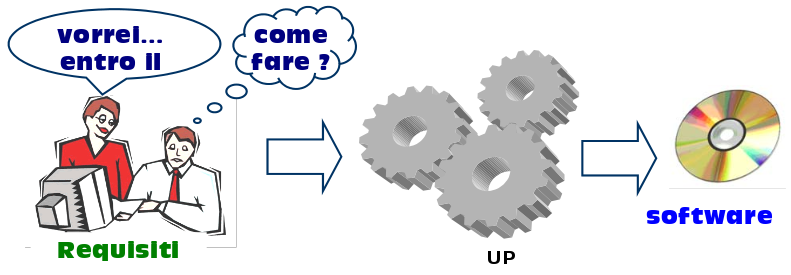
\includegraphics[scale=0.40]{image/Up_sep.png}{\centering}
    \caption{Software Engineering Process} 
    \label{fig_SEP}
   \end{figure}
 \end{frame}

 \begin{frame} {Struttura di UP}
    Il ciclo di vita del progetto è diviso in quattro fasi: Principio (Inception), Elaborazione (Elaboration), Costruzione (Construction)
    e Transizione (Transition), come si può vedere nella figura \ref{fig_US}. 
   \begin{figure}
     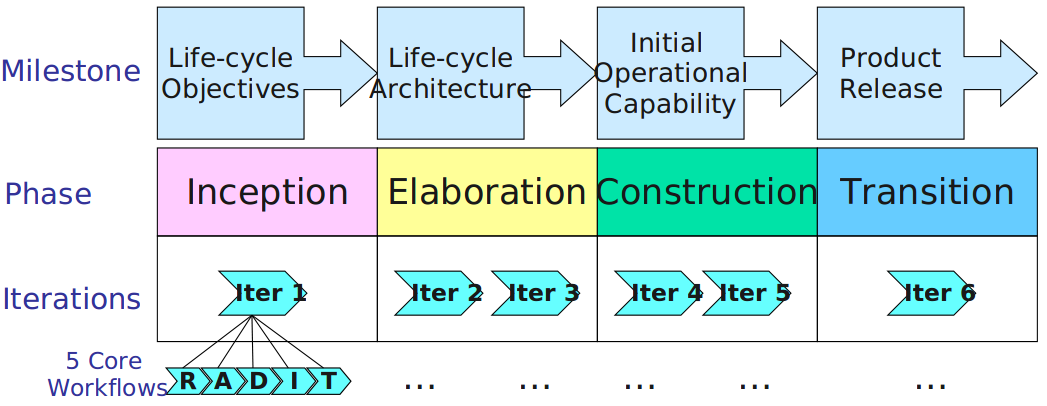
\includegraphics[scale=0.26]{image/Up_Structure.png}{\centering}
    \caption{Fasi dell'Unified Process} 
    \label{fig_US}
   \end{figure}
  \end{frame}

 \begin{frame} {Struttura di UP}
   Ogni fase è formata da una o più iterazioni. Per ogni iterazione si sviluppano in modo iterativo e incrementale 5 attività di lavoro 
   (workflows) RADIT: Requisiti (Requirements), Analisi (Analsys), Progettazione (Design), Implementazione (Implementation)e Test, come si 
   può vedere nella figura \ref{fig_UIW}.
   \begin{figure}
     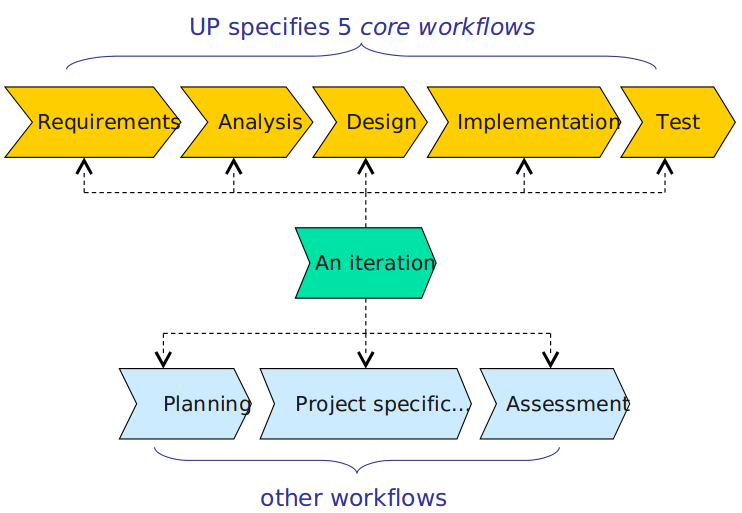
\includegraphics[scale=0.20]{image/Up_Iteration_Workflows.png}{\centering}
    \caption{Iterazioni dell'Unifiled Process} 
    \label{fig_UIW}
   \end{figure}
  \end{frame}

 \begin{frame} [allowframebreaks] {Documenti del progetto realizzati }
   Gli elementi che costituiscono il progetto realizzato sono:
   \begin{enumerate} 
     \item Documento di Visione;
     \item Glossario;
     \item Diagrammi dei casi d'uso;
     \item Identificazione e descrizione dei casi d'uso in formato breve e dettagliato;
     \item Prototipo UI (User Interface);
     \item Modello, Oggetti e Diagramma di Sequenza di dominio del sistema dei vari casi d'uso in formato dettagliato;
     \item Contratti delle operazioni;
     \item SSD e DCD di progetto del sistema dei vari casi d'uso in formato dettagliato;
     \item Codice sorgente dei diagrammi UML realizzati con Astah;
     \item Software del progetto che comprende i casi d'uso in fomato dettagliato scritto in lingaggio a oggetti Java, 
           con l'utilizzo di NetBeans IDE 8.0;
     \item Test del software realizzati tramite JUnit 4.0; 
     \item Documentazione tramite la Javadocs del codice sorgente; 
     \item Guida utente dell'avvio e configurazione del software realizzato;
     \item Documenti di istallazione, downloading dei repository di GitHub;
     \item Documentazione realizzata in \LaTeX.
   \end{enumerate}
 \end{frame}

\section{Ideazione - Iterazione 1}
 \begin{frame}[allowframebreaks] 
  \frametitle {Descrizione realtà d'interesse} 
   Nel Piano Nazionale della Ricerca (PNR)  messo a punto da HORIZON ITALIA e MIUR viene bandito un progetto chiamato:\newline
   \textbf{\virgolette{Smart Network University Communications (SNUC)}} destinato a tutti gli atenei italiani.\newline 
   Tale progetto è caratterizzato dalle seguenti specifiche descritti nel seguito, che consente ad appassionati, studenti,    
   ricercatori, docenti e imprese di scambiarsi messaggi in tempo reale su condivisioni, integrazioni e competenze di idee per una contaminazione tra ambiti 
   disciplinari diversi, realtà diverse e stimolare nei partecipanti lo sviluppo della  cultura dell’intraprendere e dell’innovazione.\newline 
   In tale sistema si richiedono le seguenti specifiche:
   \begin{itemize} 
    \item Esistono diversi canali o stanze virtuali (ciascuna legata a un corso di laurea per ogni facoltà, includendo sia la triennale e la magistrale di quel 
          determinato corso di laurea) nelle quali un utente può entrare per scambiare messaggi con gli altri utenti presenti nella stessa stanza.
    \item \`E possibile inviare due tipi di messaggi: 
          \setbeamertemplate{itemize items}[triangle]
          \begin{itemize} 
            \item \virgolette{pubblici}: dei messaggi inviati da un utente e trasmessi a tutti gli altri partecipanti presenti nella stanza; 
            \item \virgolette{privati}: dei messaggi inviati da un utente e trasmessi ad uno specifico partecipante presente nella stessa stanza, in questo caso il 
                                        destinatario selezionato sarà l’unico a ricevere il messaggio.
          \end{itemize}
          \setbeamertemplate{itemize items}[circle]
    \item In ogni istante il sistema prevede la presenza di una tipologia di utente particolare, chiamato amministratore. I compiti più importanti di un 
          amministratore sono i seguenti: 
          \setbeamertemplate{itemize items}[triangle]
          \begin{itemize} 
            \item può creare o eliminare stanze del servizio di messaggistica; 
            \item inviare messaggi di avviso ad un utente;
            \item in caso di comportamenti irregolari è possibile espellere un utente dalla stanza e l'utente non può più rientrare fin quando questo non sarà
                  rimosso dalla lista dei partecipanti bannati della stanza presente nel sistema.
          \end{itemize}
    \item Il sistema deve mandare dei messaggi di notifica, che permettono di aggiornare l’utente di un cambiamento dello stato del sistema.
  \end{itemize}
\end{frame}

\subsection{Iterazione 1: Requisiti}
\begin{frame} [allowframebreaks]
  \frametitle{Iterazione 1: Requisiti - Documento di Visione}
   La caratteristica principale del progetto è quella di consentire ad appassionati, studenti, ricercatori, docenti e imprese di scambiarsi messaggi in tempo reale   
   per ogni ateneo.  In particolare in questo progetto sono presenti diverse stanze virtuali che rappresentano le facoltà di un ateneo con due tipologie di    
   utilizzatori di sistema, ovvero l’amministratore e gli utenti del servizio di messaggistica.  Con le seguenti  caratteristiche:
   \begin{itemize} 
    \item l’amministratore gestisce le stanze virtuali e supervisiona gli utenti del servizio;
    \item gli utenti per usufruire di tale servizio inseriscono un nickname e si collegano al server impostando dei parametri di connessione. Ogni utente può    
          accedere a una stanza e inviare messaggi ad ogni utente presente nella stanza in tempo reale, inoltre ognuno può contattare in maniera privata gli altri 
          partecipanti presenti nella stanza.
   \end{itemize}
   L’architettura utilizzata per offrire il servizio è di tipo client-server, questo approccio consente di fornire un’interfaccia  più flessibile per l’accesso al   
   servizio di messaggistica anche con un semplice browser, senza modificare pesantemente la progettazione rispetto ad un architettura peer-to-peer. 
\end{frame}

\begin{frame}
  \frametitle{Iterazione 1: Requisiti - Diagrammi dei casi d'uso}
   \begin{figure}[h]
    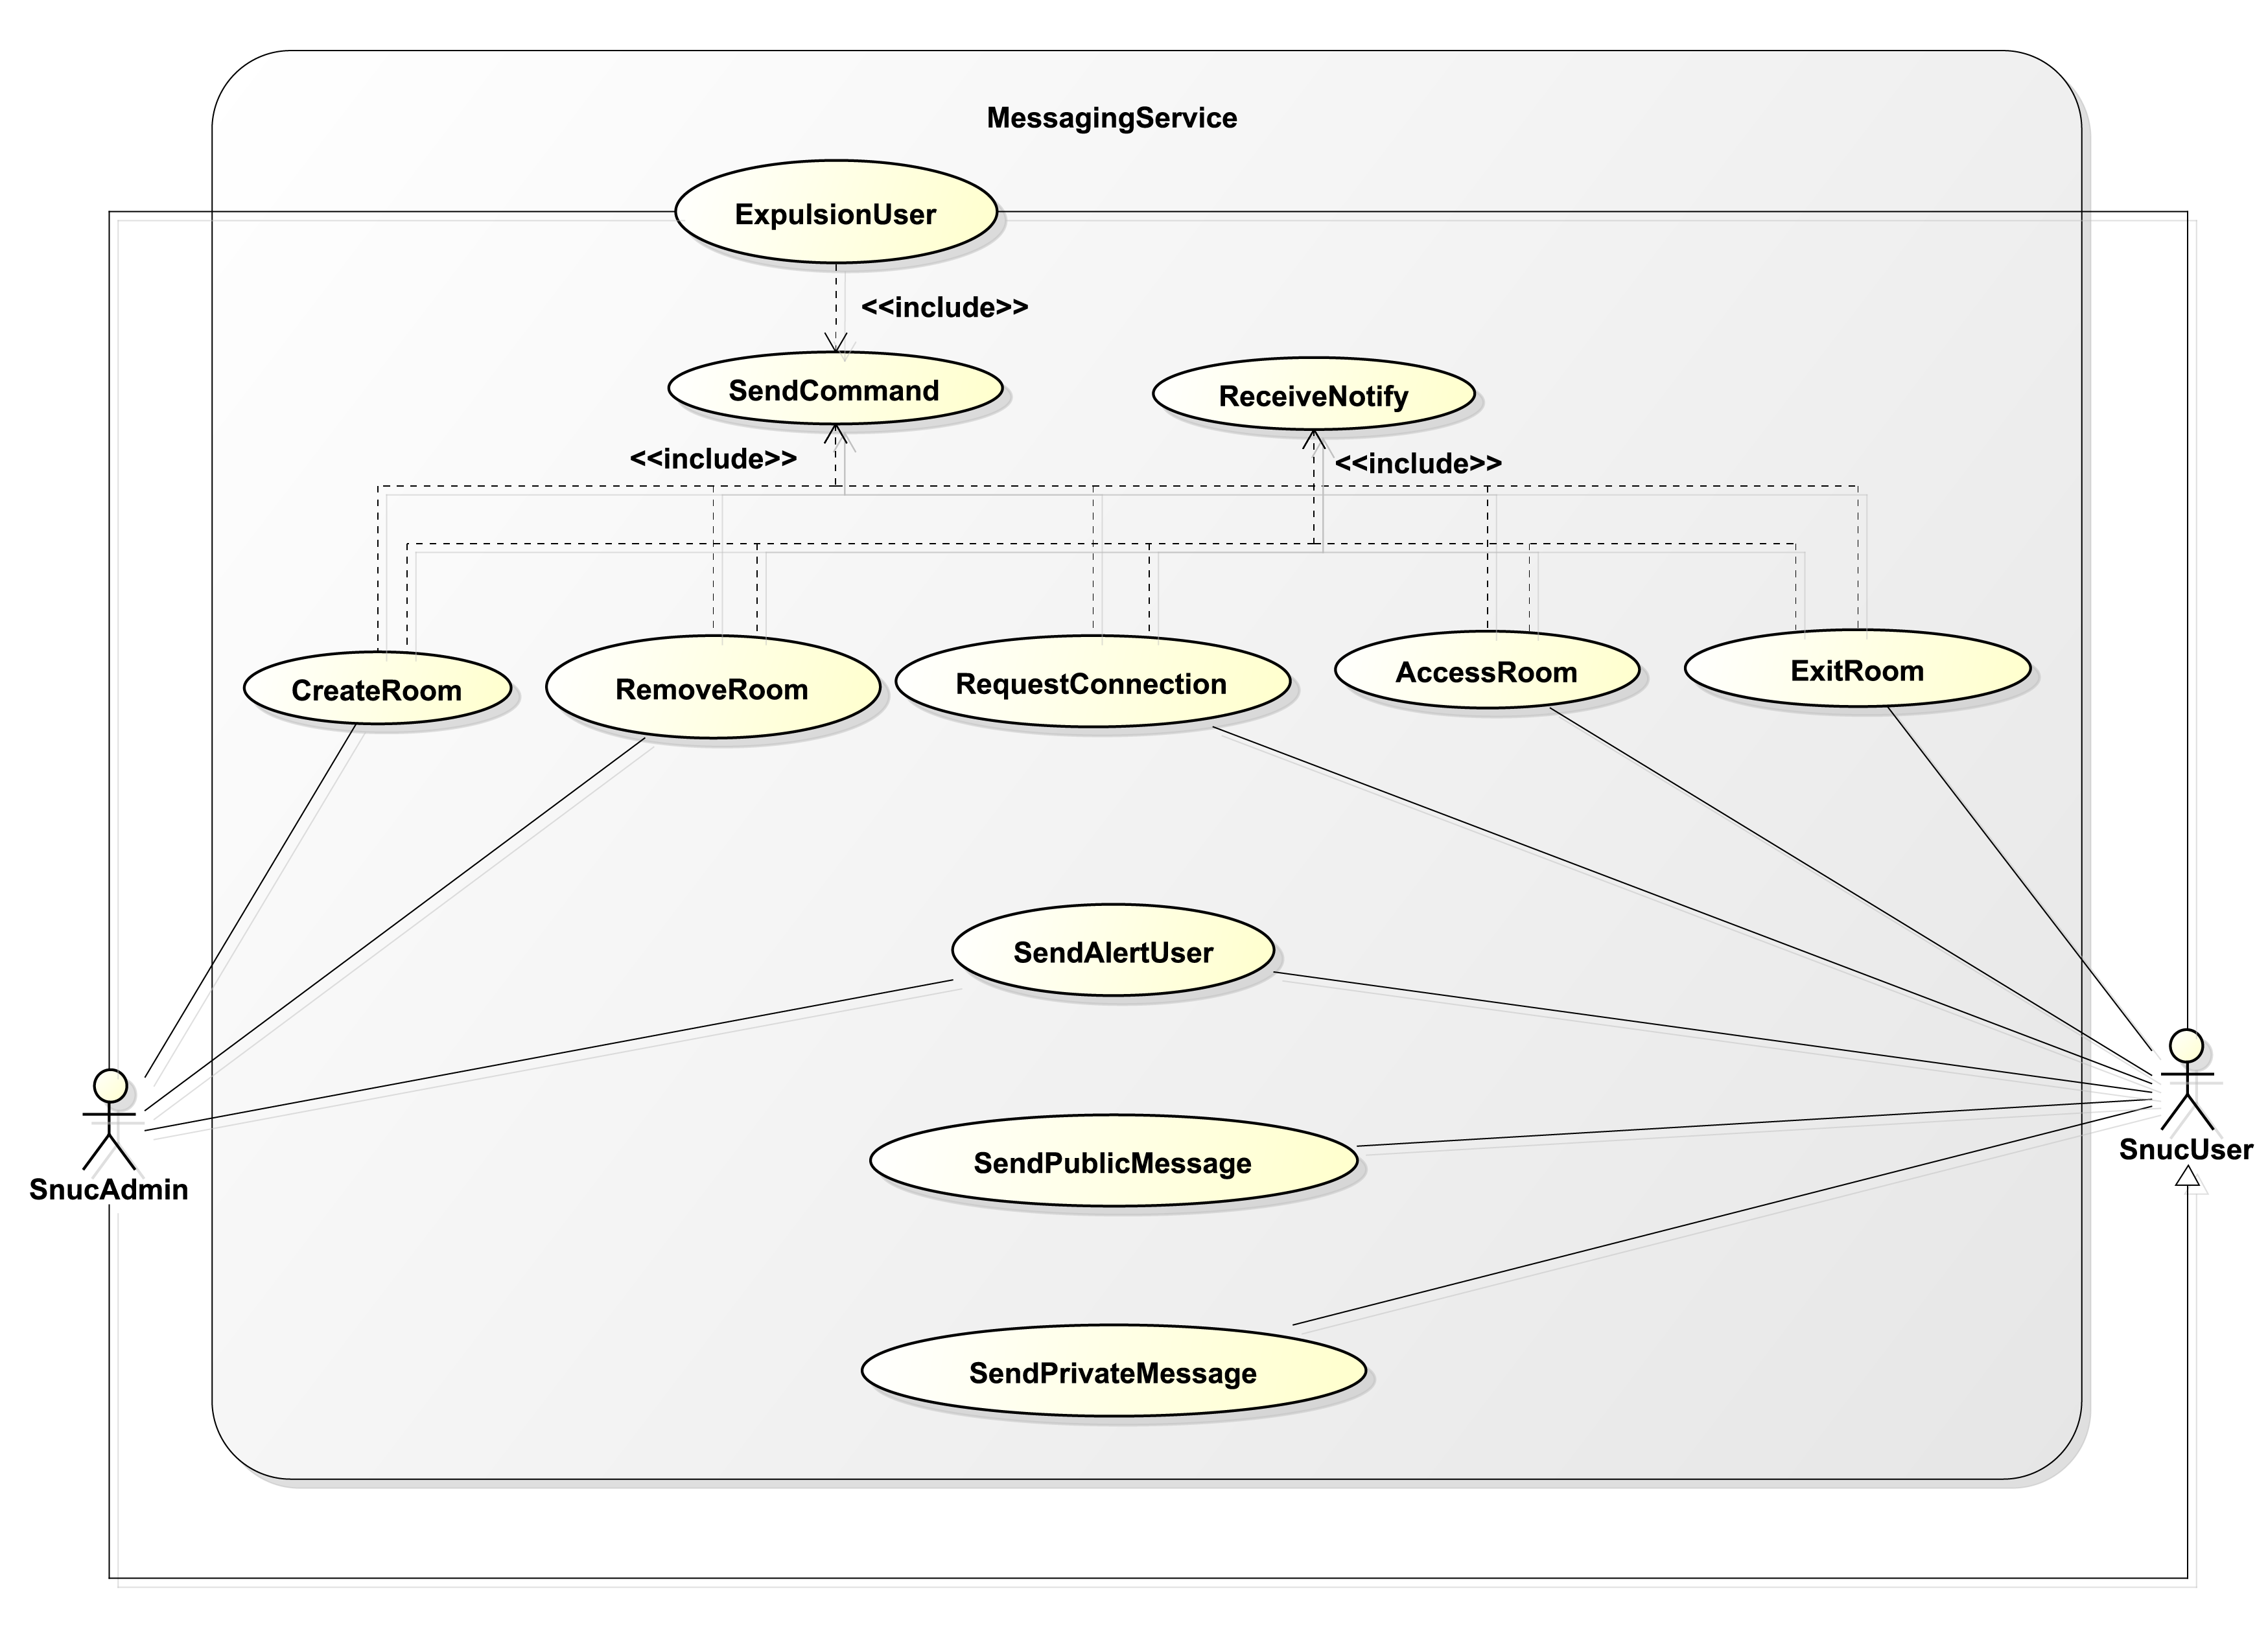
\includegraphics[scale=0.145]{image_astah/UseCaseDiagram.png}{\centering}
    \caption{Diagrammi dei casi uso} 
    \label{fig_UCD}
   \end{figure}
\end{frame}

\begin{frame} [allowframebreaks]
  \frametitle{Iterazione 1: Requisiti - Modello dei casi d'uso}
   \underline{Attori Identificati}: Amministratore (SnucAdmin) e Utente del Servizio di Messaggistica (SnucUser). \newline
   \underline{Casi d'uso identificati}: RequestConnection, AccessRoom, SendPublicMessage, SendPrivateMessage, ReceiveNotify, SendCommand, ExitRoom, CreateRoom, 
                                        RemoveRoom, SendAlertUser, ExpulsionUser. \newline
   Descrizione breve dei casi d'uso identificati:
   \begin{enumerate} 
    \item \textbf{RequestConnection}. L’utente si connette al sistema specificando il nickname, l’indirizzo e la porta del servizio di messaggistica.
    \item \textbf{AccessRoom}. L’utente richiede al sistema l’ingresso in una specifica stanza del servizio (che deve essere stata precedentemente creata 
          dall’amministratore del servizio). 
    \item \textbf{SendPublicMessage}. Il partecipante al servizio di messaggistica invia un messaggio ``pubblico'' che viene inviato dal sistema a tutti i 
          partecipanti che si trovano nella stessa stanza di colui che ha inviato il messaggio.
    \item \textbf{SendPrivateMessage}. Il partecipante al servizio di messaggistica  invia un messaggio ``privato'' ad uno specifico partecipante.
    \item \textbf{ReceiveNotify}. Il sistema manda dei messaggi di notifica, che permettono di aggiornare l’utente di un cambiamento dello stato del sistema.
    \item \textbf{SendCommand}. Il sistema è in grado di ricevere e interpretare dei comandi.
    \item \textbf{ExitRoom}. Un partecipante richiede al sistema l’uscita dal servizio. Questo comporta la sua eliminazione dall’insieme dei partecipanti presenti 
          nella stanza del servizio cui era precedentemente associato l’utente.
    \item \textbf{CreateRoom}. L’amministratore del servizio di messaggistica è responsabile della creazione (preventiva) delle stanze che potranno successivamente 
          essere visitate dai partecipanti.
    \item \textbf{RemoveRoom}. In ogni momento l’amministratore può eliminare una stanza dal servizio (ad esempio perchè non ci sono partecipanti). Ciò comporta 
          l’invio preventivo di un messaggio a tutti i patecipanti eventualmente presenti nella stanza, i quali potranno in seguito richiedere l’ingresso in una   
          nuova stanza del servizio.
    \item \textbf{SendAlertUser}. L’amministratore può in ogni momento inviare un messaggio di avviso ad uno specifico partecipante al servizio.
    \item \textbf{ExpulsionUser}. L’amministratore può in ogni momento espellere da una stanza uno specifico partecipante.  
   \end{enumerate}
\end{frame}

\setbeamertemplate{itemize items}[triangle]
\begin{frame} [allowframebreaks]
  \frametitle{Glossario} 
   \begin{itemize} 
    \item SnucUser, User, Utente: è l'utente del servizio di messaggistica che è in grado di registrarsi a delle stanze, di inviare messaggi pubblici e privati.
    \item SnucAdmin, Admin, Amministratore: è il gestore del servizio di messaggistica, che possiede la facoltà di creare e/o eliminare una stanza, di inviare un 
          particolare messaggio di avviso ad un partecipante per un comportamento non corretto ed eventualmente di bannarlo eliminandolo dalla stanza.
    \item Messaging Service, Servizio di messaggistica, sistema, chat: sistema che si occupa della gestione.
    \item Room, stanza, canale: rappresenta un luogo virtuale, dove gli utenti possono scambiarsi informazioni relative alle tematiche trattate.
    \item Messaggio Pubblico: messaggio testuale inviato da un partecipante a tutti gli utenti presenti nella stanza.
    \item Messaggio Privato: messaggio testuale inviato da un partecipante ad un particolare partecipante presente nella stanza.
    \item Notifica: particolari messaggi di avviso inviati dal server agli utenti che usufruiscono del servizio.  
  \end{itemize}
\end{frame}

\subsection{Iterazione 1: Requisiti - UC1\_RequestConnection}
\begin{frame}
 \frametitle{Iterazione 1: Requisiti - UC1\_RequestConnection}
  \begin{table}[!htbp]
     \caption {Descrizione dettagliata: caso d'uso UC1\_RequestConnection}
     \label{table_UC1_RC}
     \resizebox{\linewidth}{!}{%
      \begin{tabular}{|l|p{10cm}|}\hline
       Nome caso d'uso &  UC1\_RequestConnection \\\hline
       Portata & Applicazione Smart Intelligent University Communications \\\hline
       Livello &  Obiettivo Utente \\\hline
       Attore primario &  SnucUser \\\hline
       Parti interessate e interessi &  SnucUser: vuole collegarsi al servizio di messaggistica \\\hline
       Pre-condizioni & L'utente ha bisogno di una connessione di rete\\\hline
       Post-condizioni (garanzia di successo) &  L'utente è inserito tra gli utenti online con il nickname confermato dal servizio di messaggistica ottenendo un 
                                                 messaggio di benvenuto \\\hline
       Scenario principale di successo &  
       \begin{enumerate} 
        \item L'utente inserisci un nickname, l'address e la porta del server.
        \item Il sistema esamina il nickname inviato dall'utente e verifica se è presente una omonimia.
        \item Il sistema conferma l'inserimento tra gli utenti online inviando una notifica di benvenuto.
       \end{enumerate} \\\hline
      \end{tabular}}
   \end{table}
\end{frame}

\begin{frame}
 \frametitle{Iterazione 1: Requisiti - UC1\_RequestConnection}
  \begin{table}[!htbp]
      \resizebox{\linewidth}{!}{%
       \begin{tabular}{|l|p{10cm}|}\hline
         Estensioni (o flussi alternativi) &  
           1A - SnucUser inserisce parametri errati: 
          \begin{itemize} 
           \item Viene visualizzato un messaggio di errore e viene richiesto nuovamente l’inserimento di tali parametri.
          \end{itemize} 
           2A - Omonimia del nickname:
          \begin{itemize}       
           \item Il sistema cambia il nickname aggiungendo "\_" al nickname (es. \_nickname). 
           \item Il sistema conferma l'inserimento tra gli utenti online inviando una notifica di benvenuto.
          \end{itemize} \\\hline
       Requisiti speciali (Requisiti Non Funzionali) &  Comunicazione asincrona in cui lo scambio di informazioni avviene in tempo reale, senza sensibili pause tra 
                                                        invio e ricezione del messaggio.\\\hline
       Elenco delle varianti tecnologiche &  L’applicazione dovrebbe essere flessibile al funzionamento di diversi protocolli di comunicazione (es. TCP, UDP) e con   
       diversi strati middleware (es. Socket, RMI) \\\hline
       Frequenza di ripetizione & Potrebbe essere quasi ininterrotta \\\hline
       Varie e/o Problemi Aperti &  // \\\hline
      \end{tabular}}
   \end{table}
\end{frame}

\subsection{Iterazione 1: Requisiti - UC2\_AccessRoom}
\begin{frame}
 \frametitle{Iterazione 1: Requisiti - UC2\_AccessRoom}
  \begin{table}[!htbp]
   \caption {Caso d'uso UC2\_AccessRoom}
    \label{table_UC2_AR}
     \resizebox{\linewidth}{!}{%
      \begin{tabular}{|l|p{10cm}|}\hline
       Nome caso d'uso &  UC2\_AccessRoom\\\hline
       Portata & Applicazione Smart Intelligent University Communications \\\hline
       Livello & Obiettivo Utente \\\hline
       Attore primario & SnucUser  \\\hline
       Parti interessate e interessi & SnucUser: vuole registrarsi e effettuare l’ingresso in una stanza presente nel servizio di messaggistica \\\hline
       Pre-condizioni & Nel sistema è presente almeno una stanza creata da un amministratore.\\\hline
       Post-condizioni (garanzia di successo) &  Nel caso di svolgimento normale l’utente è registrato ed è presente nell’insieme degli utenti della stanza 
                                                 specificata. \\\hline
      \end{tabular}}
   \end{table}
\end{frame}

\begin{frame}
 \frametitle{Iterazione 1: Requisiti - UC2\_AccessRoom}
  \begin{table}[!htbp]
      \resizebox{\linewidth}{!}{%
       \begin{tabular}{|l|p{10cm}|}\hline
          Scenario principale di successo &  
           \begin{enumerate} 
            \item L’utente richiede una lista di stanze presenti nel sistema  di messaggistica.
            \item Il sistema invia la lista delle stanze.
            \item L’utente seleziona la stanza tra quelle presenti in lista.
            \item Il sistema registra l’utente alla stanza.
            \item Il sistema visualizza a video gli utenti presenti nella stanza.
            \item Il sistema visualizza un’area pubblica dove vengono mostrati tutte le conversazioni in corso dal quel momento in poi. 
          \end{enumerate} \\\hline 
         Estensioni (o flussi alternativi) &  
           3A - Il SnucUser inserisce una stanza non in elenco:
          \begin{enumerate} 
           \item Il sistema invia un messaggio di errore.
          \end{enumerate} \\\hline
       Requisiti speciali (Requisiti Non Funzionali) &  Comunicazione asincrona in cui lo scambio di informazioni avviene in tempo reale, senza sensibili pause tra 
                                                        invio e ricezione del messaggio.\\\hline
       Elenco delle varianti tecnologiche &  L’applicazione dovrebbe essere flessibile al funzionamento di diversi protocolli di comunicazione (es. TCP, UDP) e con   
       diversi strati middleware (es. Socket, RMI) \\\hline
       Frequenza di ripetizione & Potrebbe essere quasi ininterrotta \\\hline
       Varie e/o Problemi Aperti &  // \\\hline
      \end{tabular}}
   \end{table}
\end{frame}

\begin{frame}{Descrizione Prototipo User Interface}
 Viene presentata un prototipo dell'interfaccia grafica (GUI) al cliente realizzata tramite Balsamiq Mockups per rendere più visibile 
 il confine del sistema di iterazione da parte delle figure coinvolte con l'ipotetico sistema da realizzare, in modo da sollevare
 ipotetiche situazioni problematiche relative. 
\end{frame} 

\begin{frame} {Iterazione 1: Requisiti - Prototipo  User Interface}
    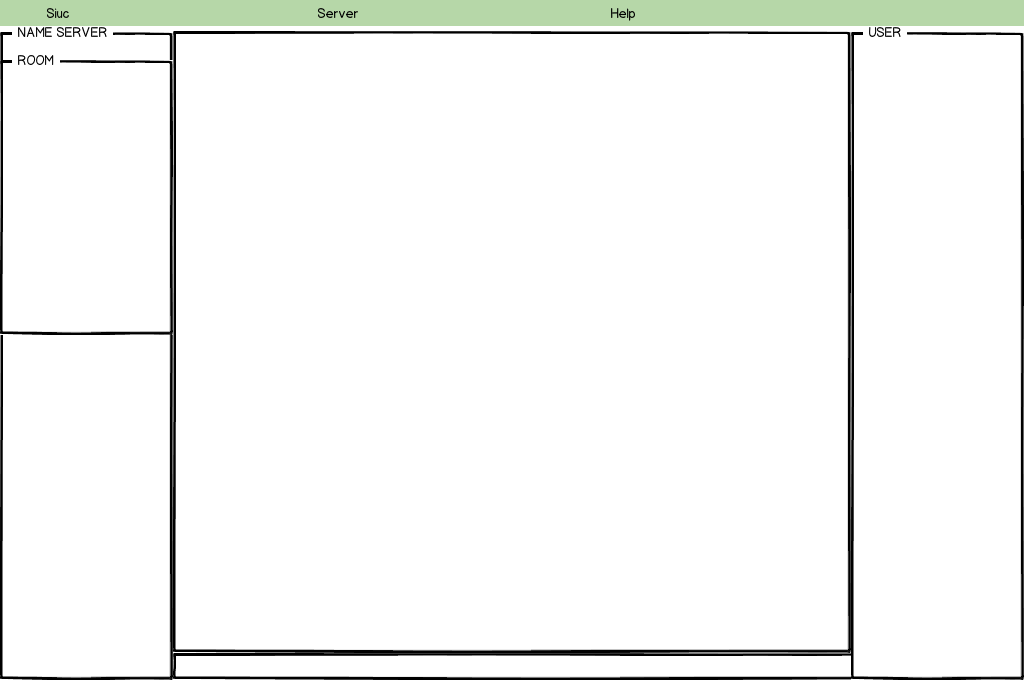
\includegraphics[scale=0.28]{image_mockups/01_snuc_open.png}{\centering}
\end{frame}

\begin{frame} {Iterazione 1: Requisiti - Prototipo User Interface}
    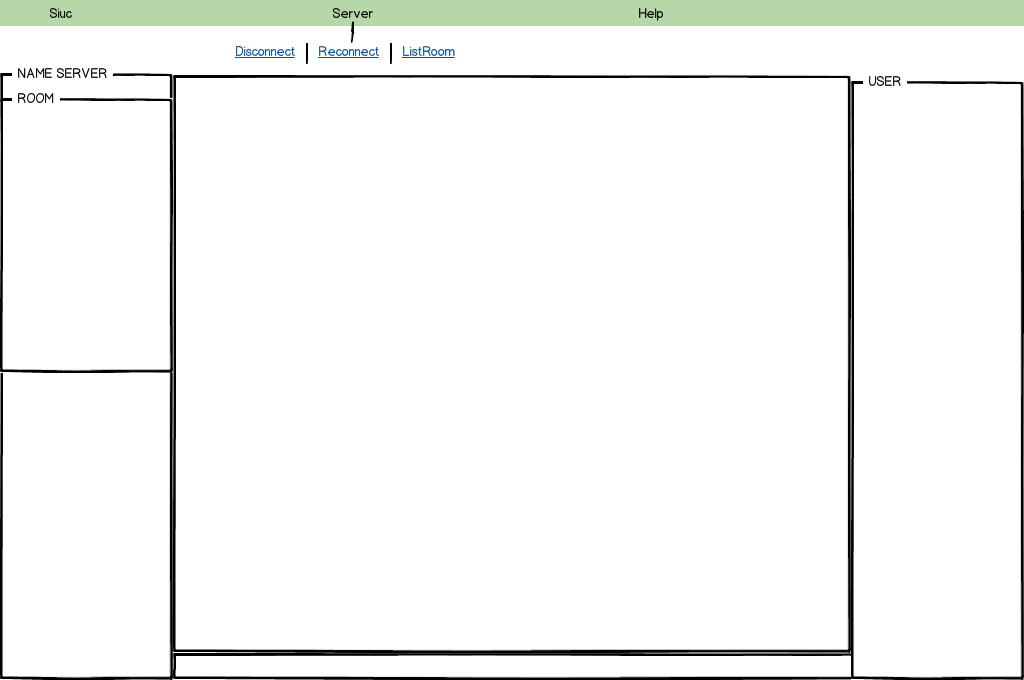
\includegraphics[scale=0.28]{image_mockups/02_snuc_menu_server.png}{\centering}
\end{frame}

\begin{frame} {Iterazione 1: Requisiti - Prototipo User Interface}
    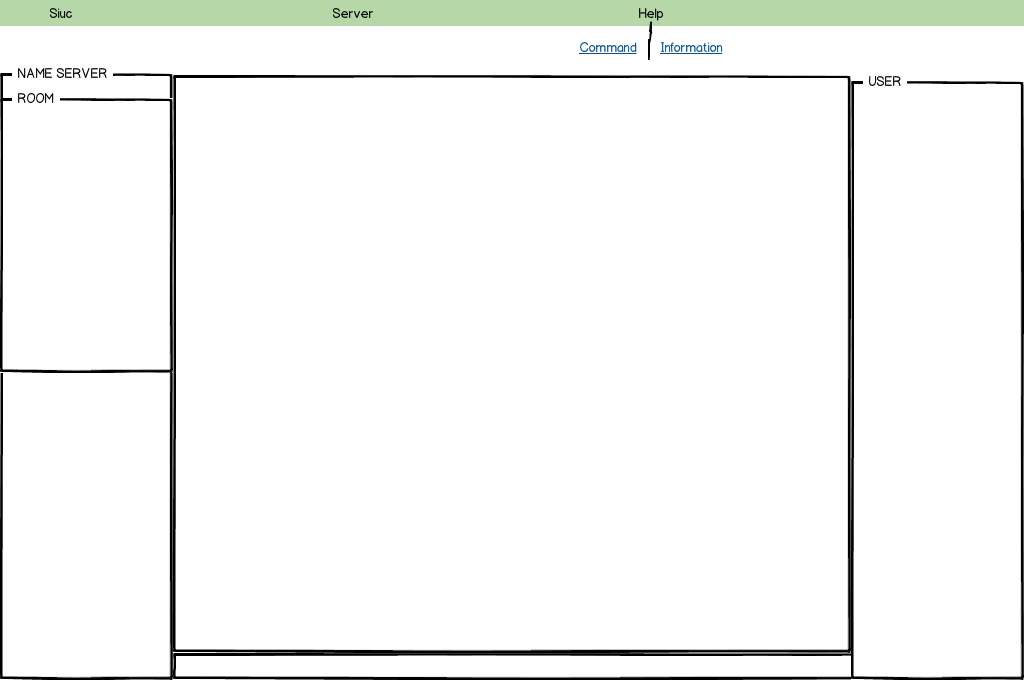
\includegraphics[scale=0.28]{image_mockups/03_snuc_menu_help.png}{\centering}
\end{frame}

\begin{frame} {Iterazione 1: Requisiti - Prototipo User Interface}
    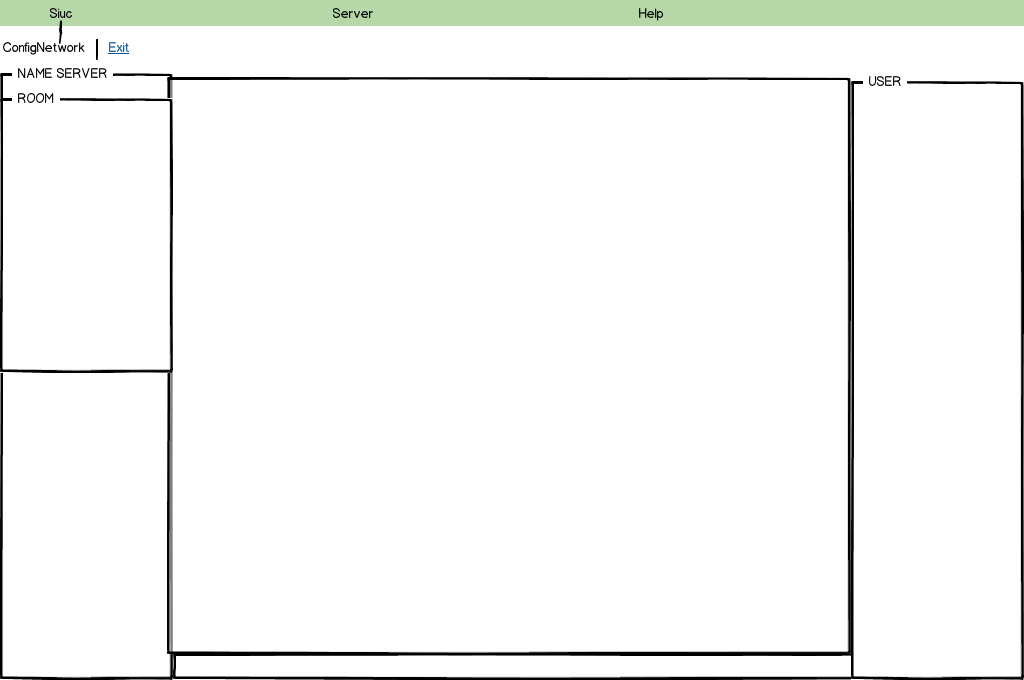
\includegraphics[scale=0.28]{image_mockups/04_snuc_menu_snuc.png}{\centering}
\end{frame}

\begin{frame} {Iterazione 1: Requisiti - Prototipo User Interface}
    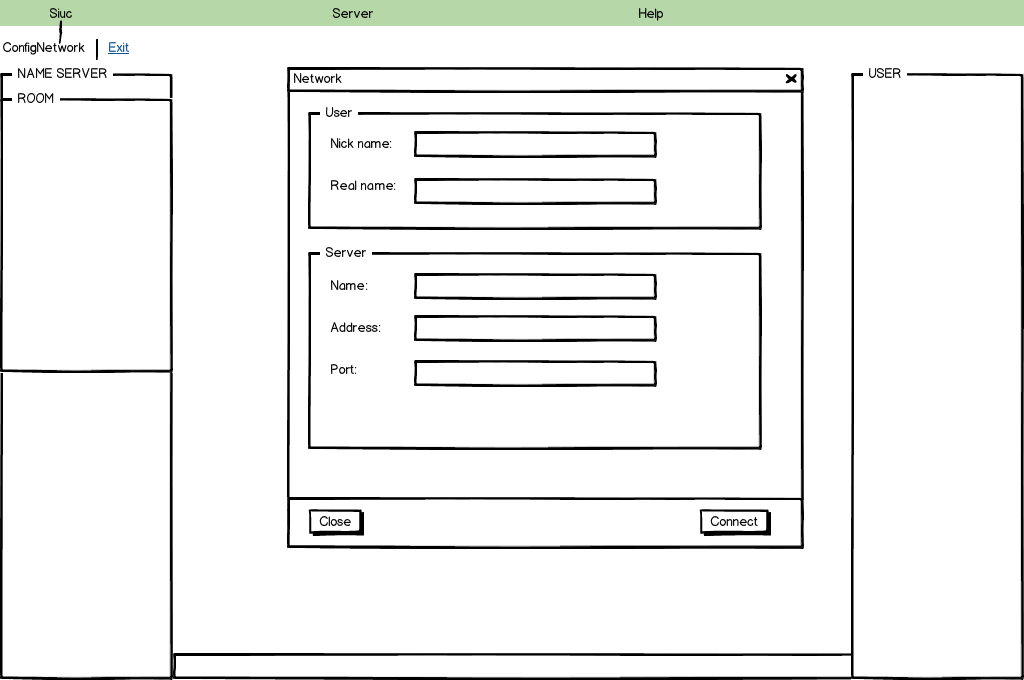
\includegraphics[scale=0.28]{image_mockups/05_snuc_config_network.png}{\centering}
\end{frame}

\begin{frame} {Iterazione 1: Requisiti - Prototipo User Interface}
    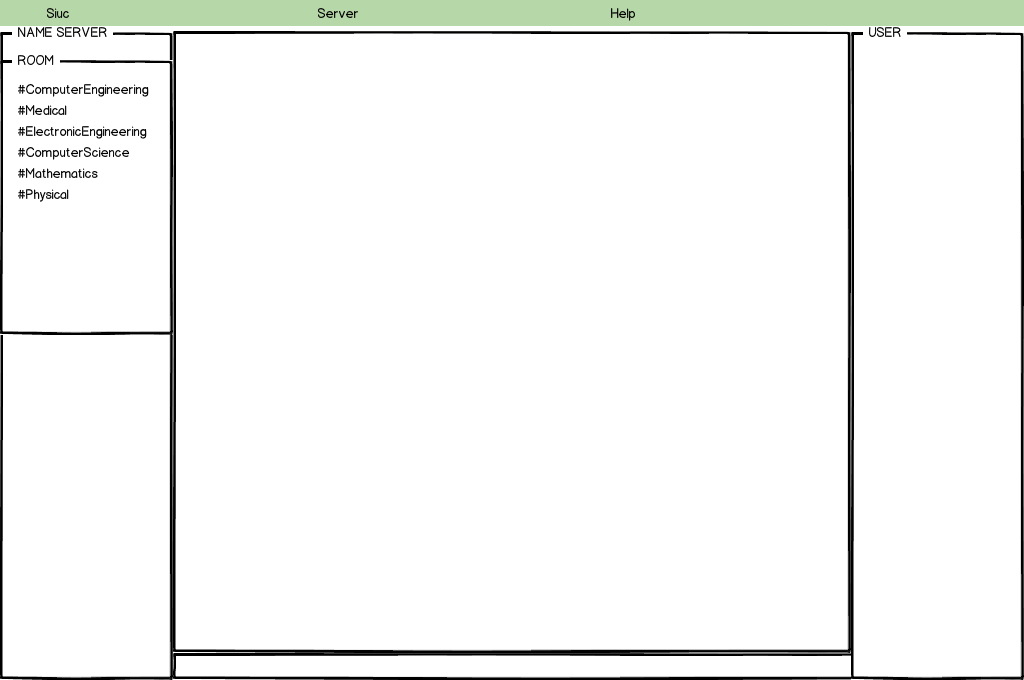
\includegraphics[scale=0.28]{image_mockups/06_snuc_connect.png}{\centering}
\end{frame}

\begin{frame} {Iterazione 1: Requisiti - Prototipo User Interface}
    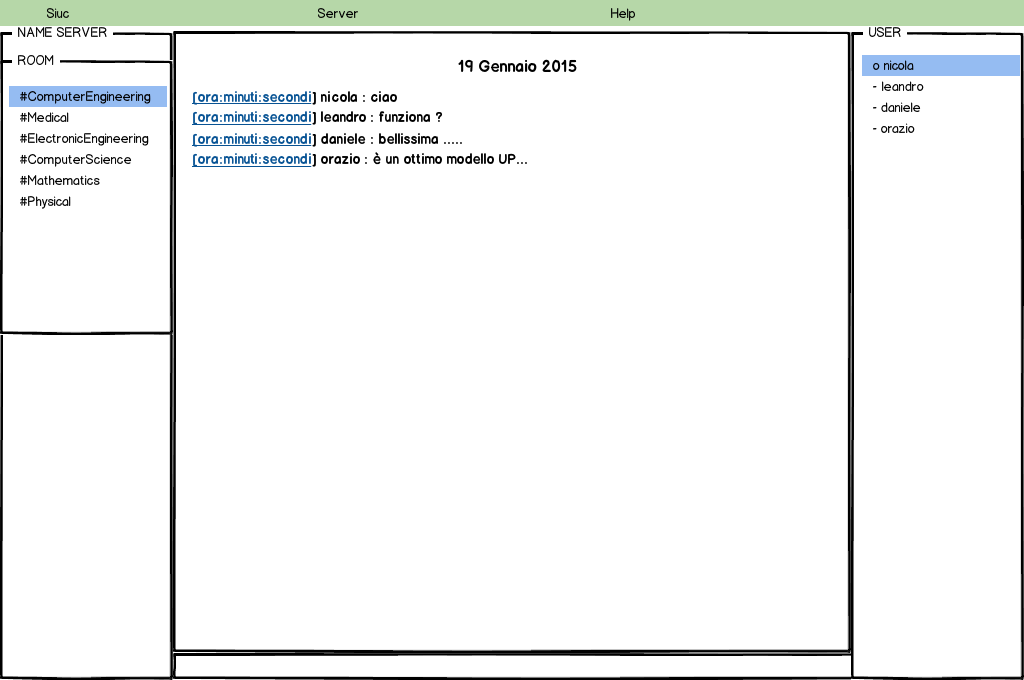
\includegraphics[scale=0.28]{image_mockups/07_snuc_user_room_ce.png}{\centering}
\end{frame}

\begin{frame} {Iterazione 1: Requisiti - Prototipo User Interface}
    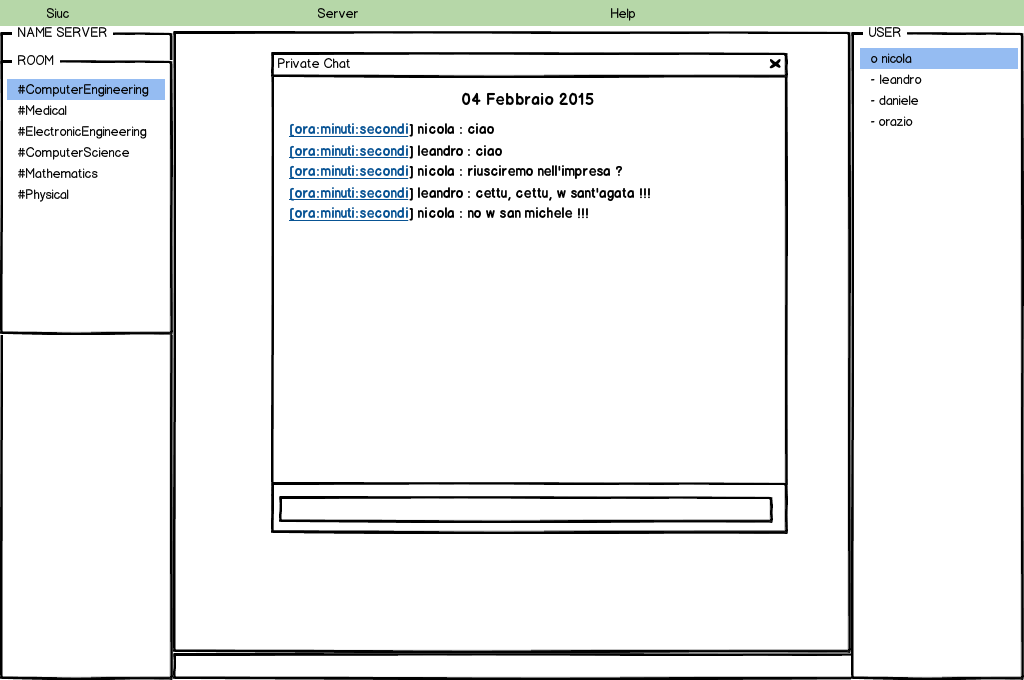
\includegraphics[scale=0.28]{image_mockups/08_snuc_user_room_ce_private.png}{\centering}
\end{frame}

\begin{frame} {Iterazione 1: Requisiti - Prototipo User Interface}
    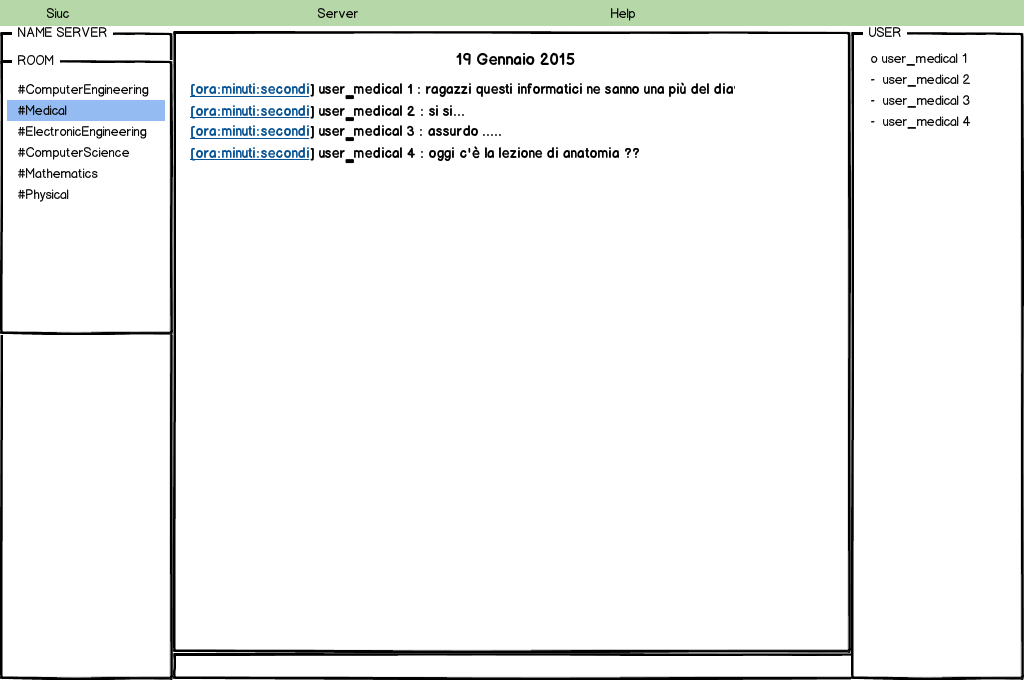
\includegraphics[scale=0.28]{image_mockups/09_snuc_user_room_medical.png}{\centering}
\end{frame}

% ANALISI ITERAZIONE 1 - UC1_RequestConnection e UC2_AccessRoom
\subsection{Iterazione 1: Analisi - UC1\_RequestConnection}
\begin{frame}[allowframebreaks] {Descrizione Analisi - UC1\_RequestConnection}
 In questa iterazione, del caso d’uso UC1 è di interesse lo scenario principale di successo.  Da esso è possibile identificare le seguenti classi concettuali: 	
 \begin{itemize}
  \item \textbf{User}: rappresenta il generico utente connesso al servizio di messaggistica. È caratterizzato da un ``nickname'' e può ricevere notifiche dal sistema 
                centrale.
  \item \textbf{MessagingService}: rappresenta ed incapsula il servizio di messaggistica nel suo complesso. Mantiene una lista di utenti connessi a tale sistema.
  \item \textbf{Message}: individua un generico messaggio scambiato tra utenti della chat o tra servizio di messaggistica e utente. È costituito da un 
               ``content'' (contenuto del messaggio), da una ``date'' (rappresenta la data) e dal ``sender'' (mittente).
  \item \textbf{Notify}: è una specializzazione del tipo Message ed è caratterizzata da un ``typeNotify'' che serve a distinguere il tipo di notifica (ad es. 
        CONNECTION\_ACCEPT nel caso in cui la connessione è stata stabilita correttamente).        
 \end{itemize}
\end{frame}

\begin{frame} {Iterazione 1: Analisi - UC1\_RequestConnection}
   \begin{figure}
     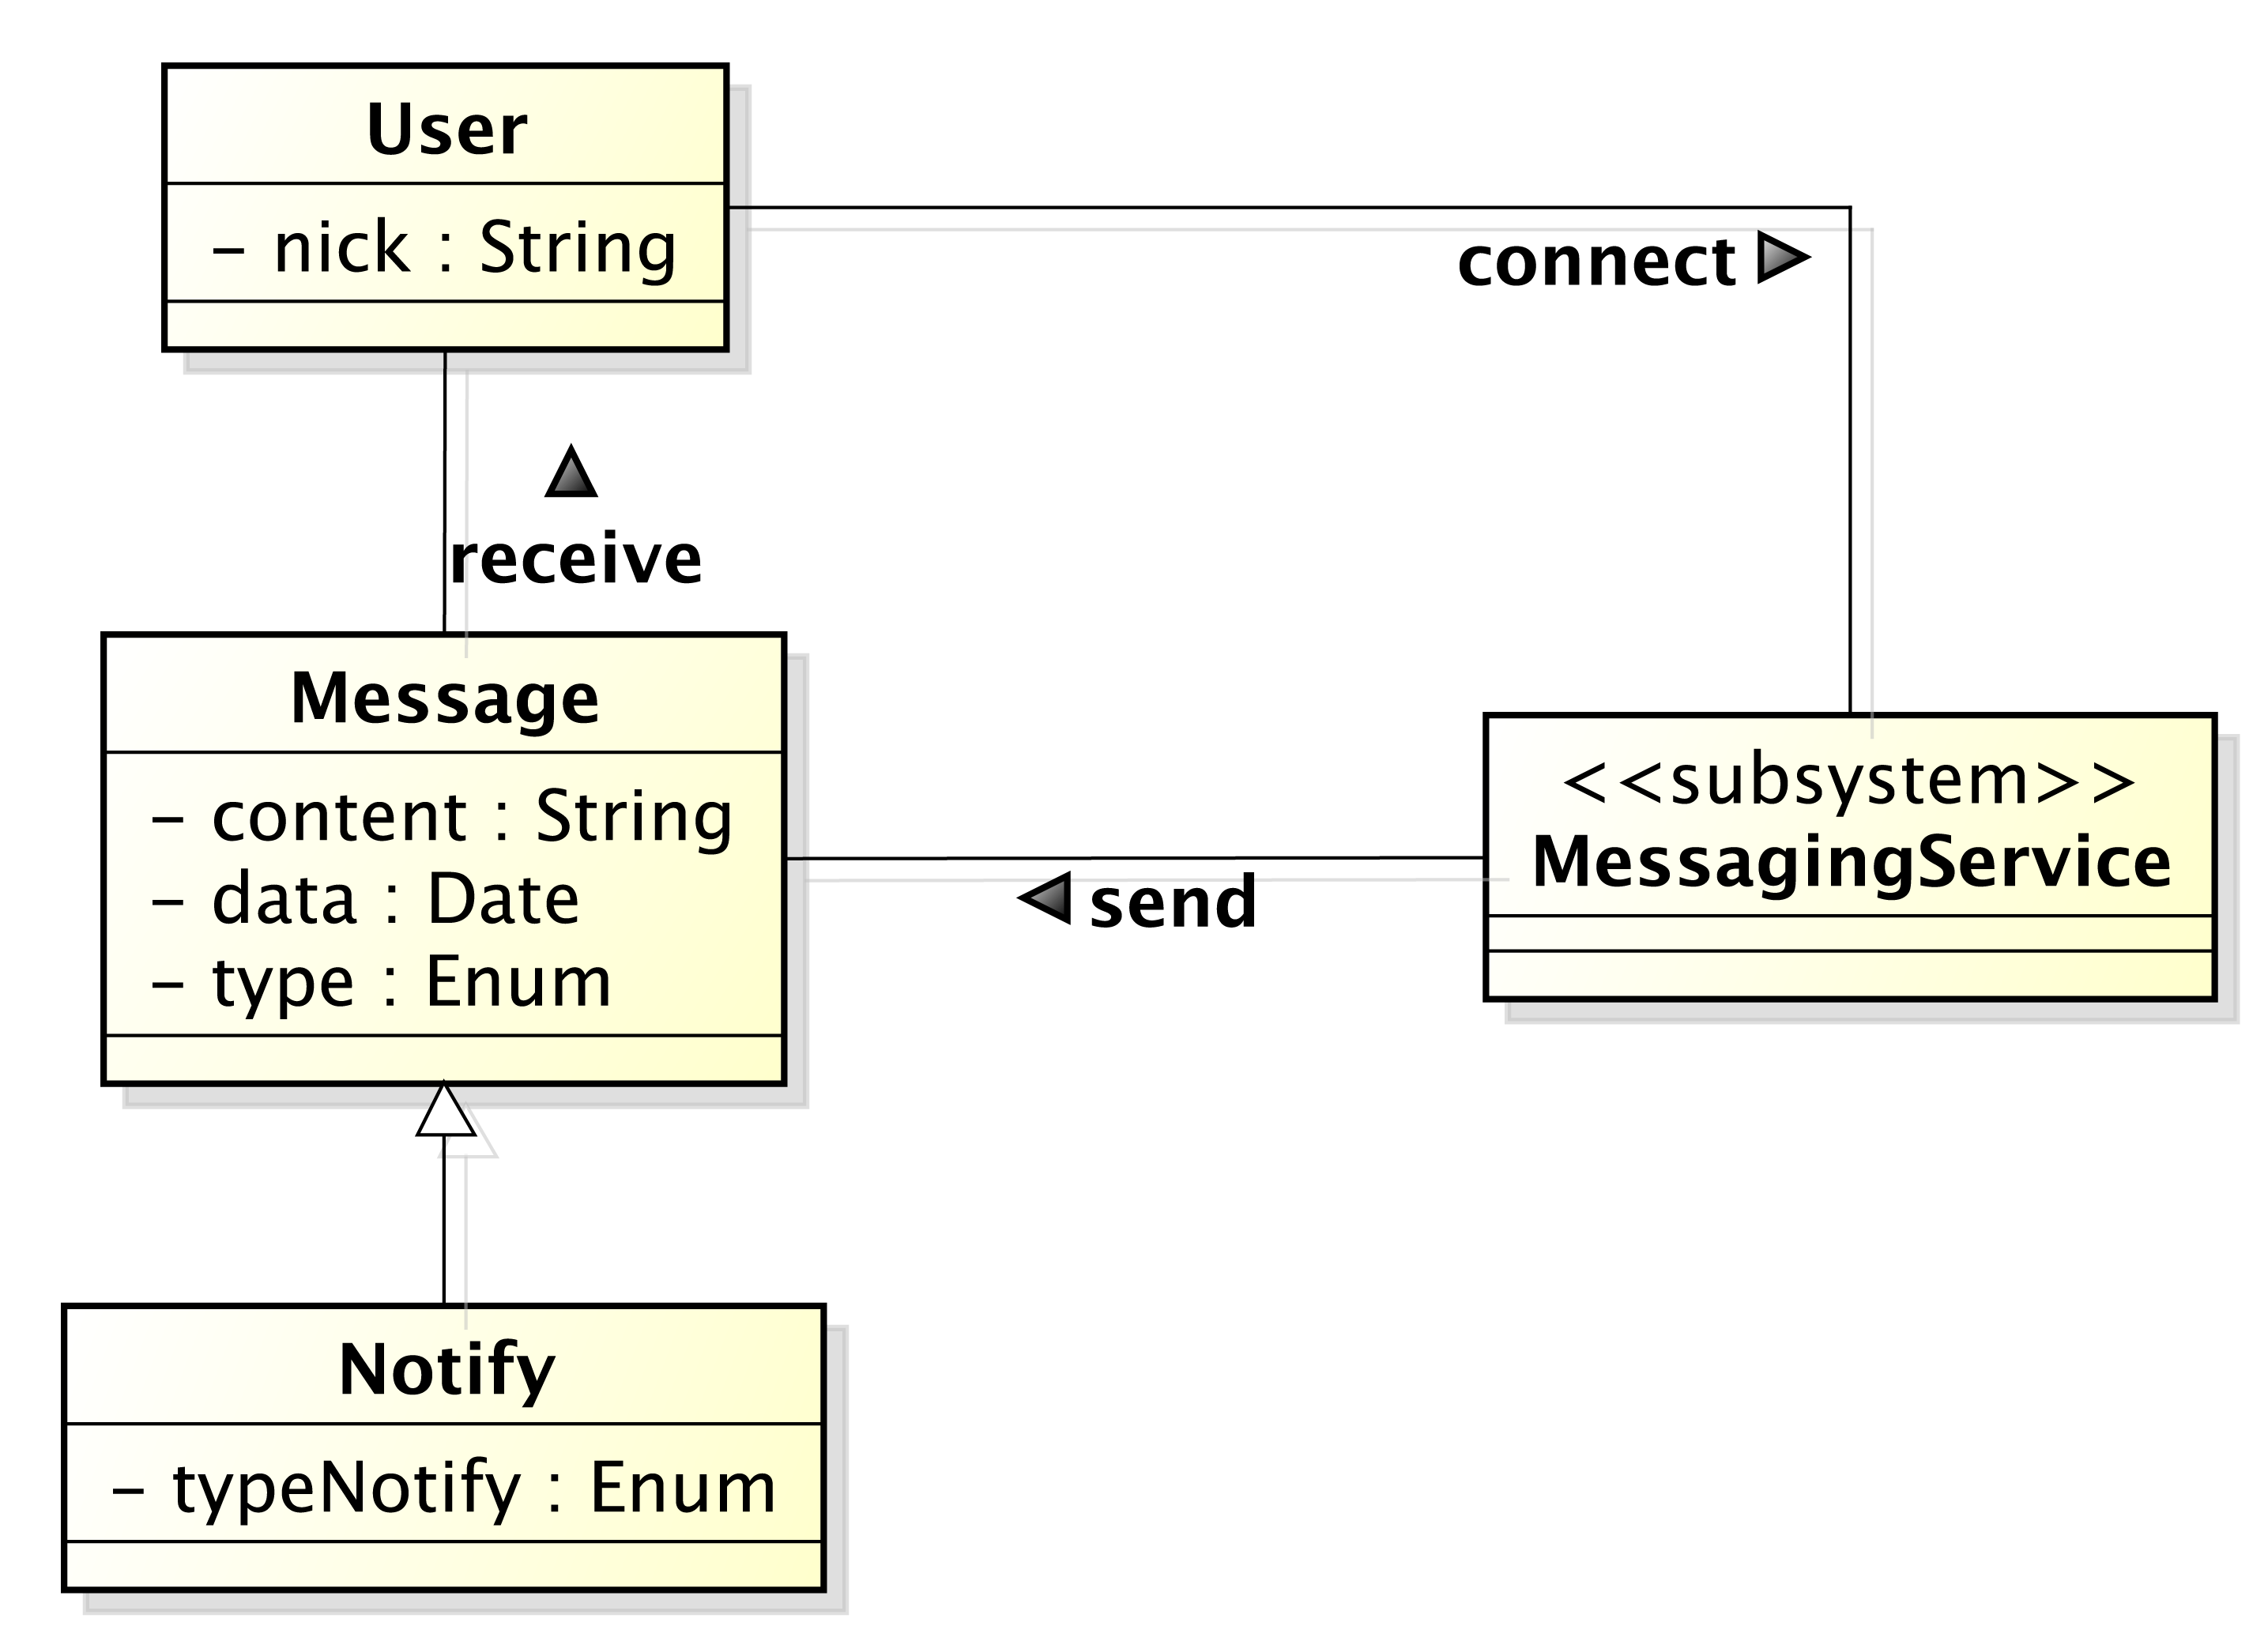
\includegraphics[scale=0.34]{image_astah/Iteration_1_DomainModel/UC1_RequestConnection_DM.png}{\centering}
     \caption{UC1 - Modello di dominio}
     \label{fig_UC1_RC_DM} 
   \end{figure}
\end{frame}

\begin{frame} {Iterazione 1: Analisi - UC1\_RequestConnection}
   \begin{figure}
     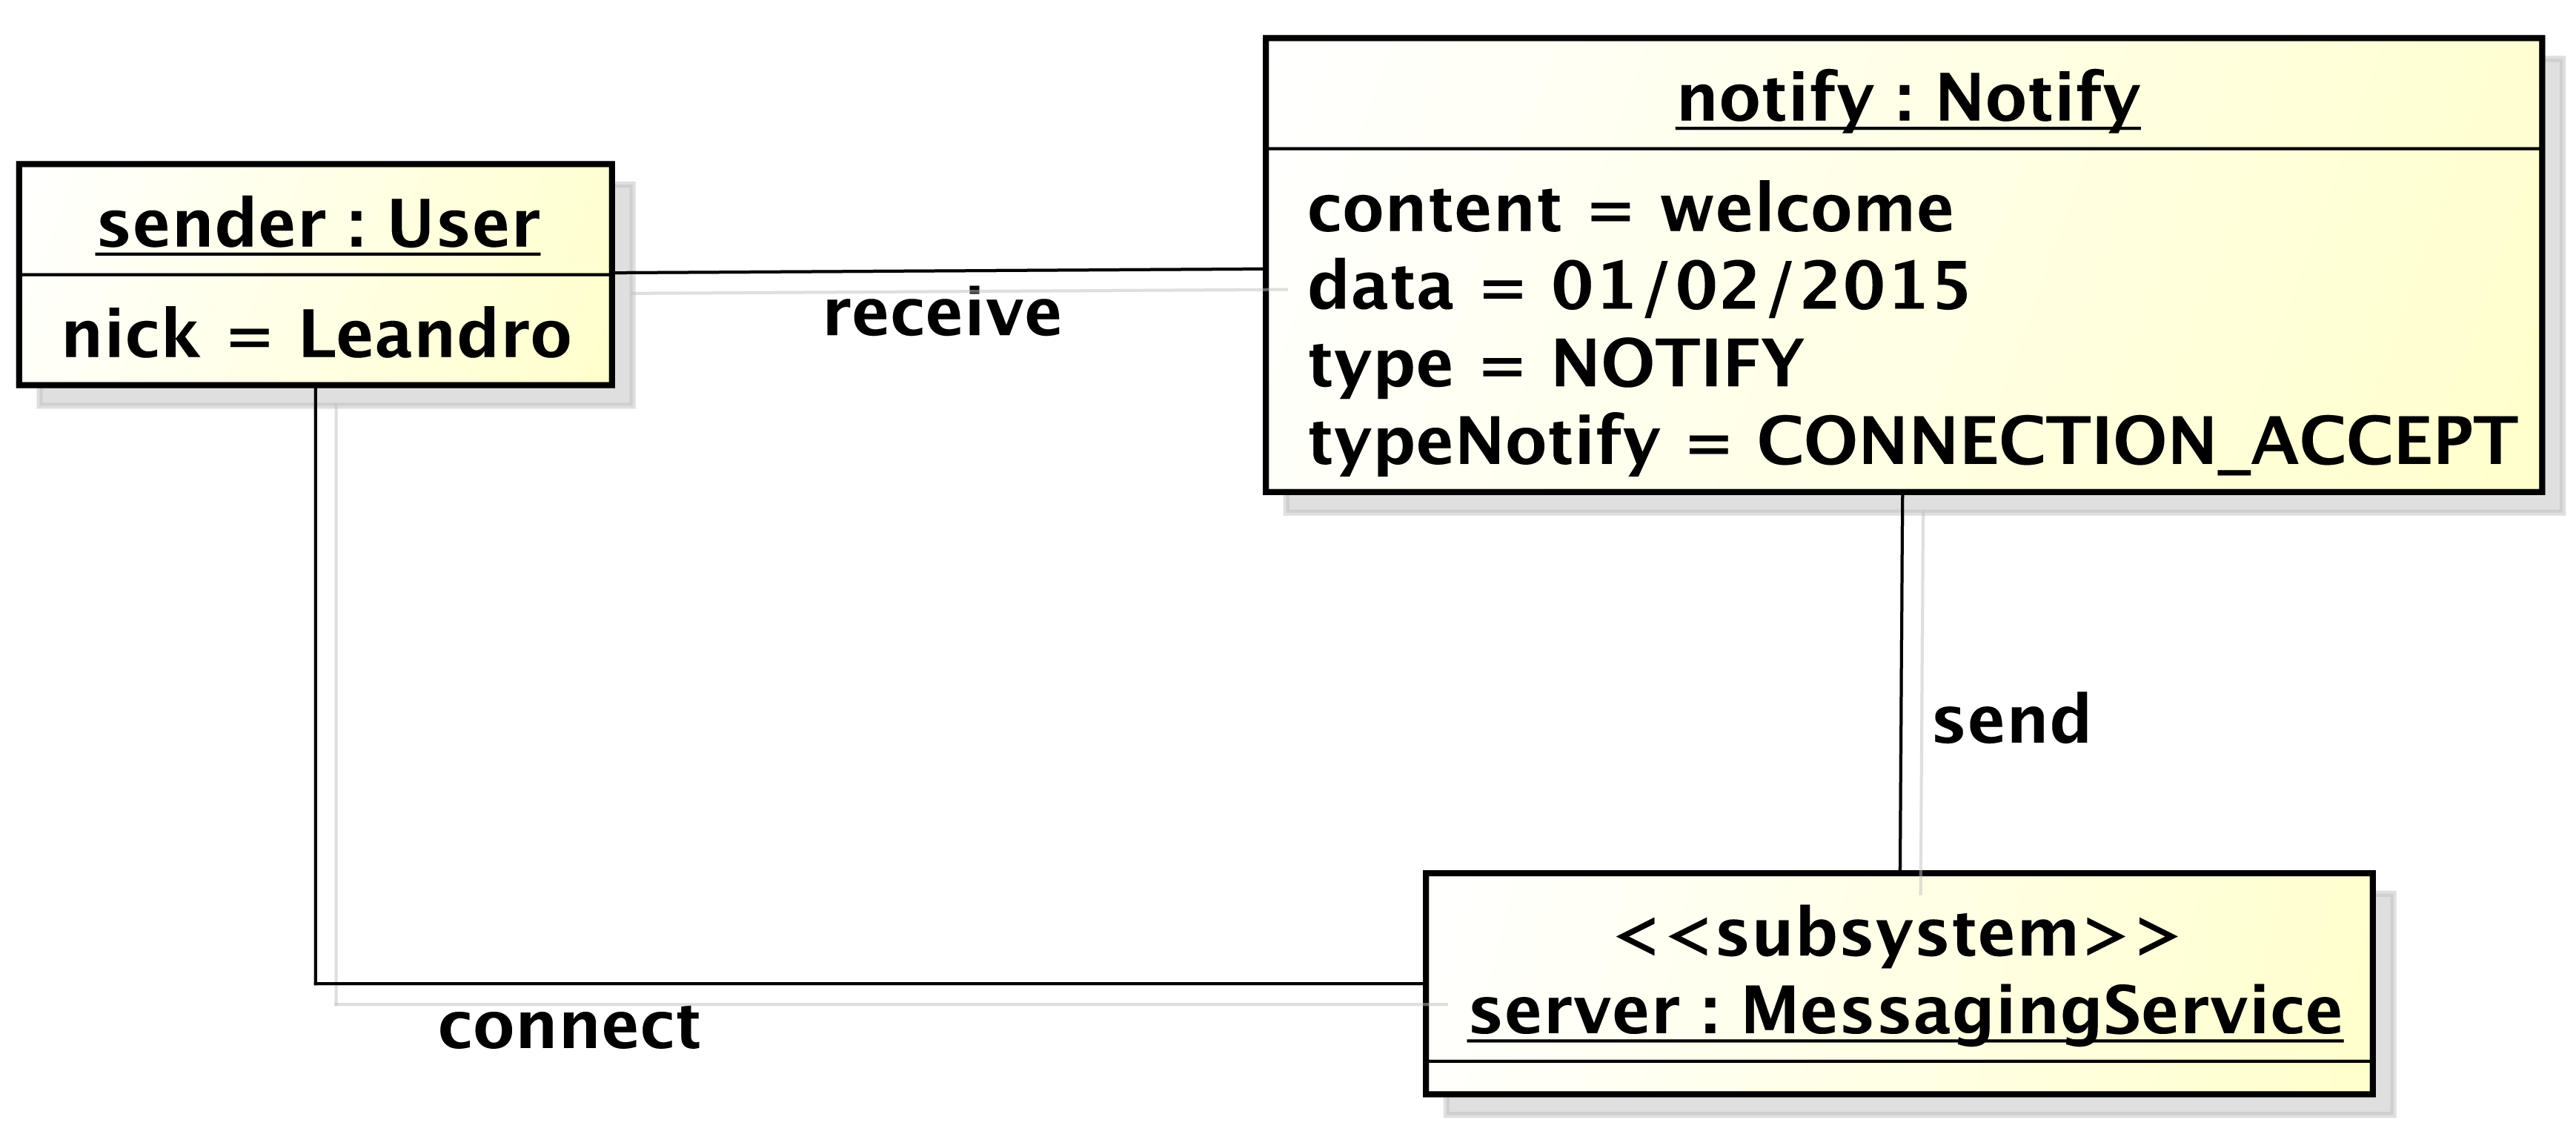
\includegraphics[scale=0.35]{image_astah/Iteration_1_DomainModel/UC1_RequestConnection_OM}{\centering}
     \caption{UC1 - Oggetti di dominio}
     \label{fig_UC1_RC_OM} 
   \end{figure}
\end{frame}

\begin{frame} {Iterazione 1: Analisi - UC1\_RequestConnection}
   \begin{figure}
     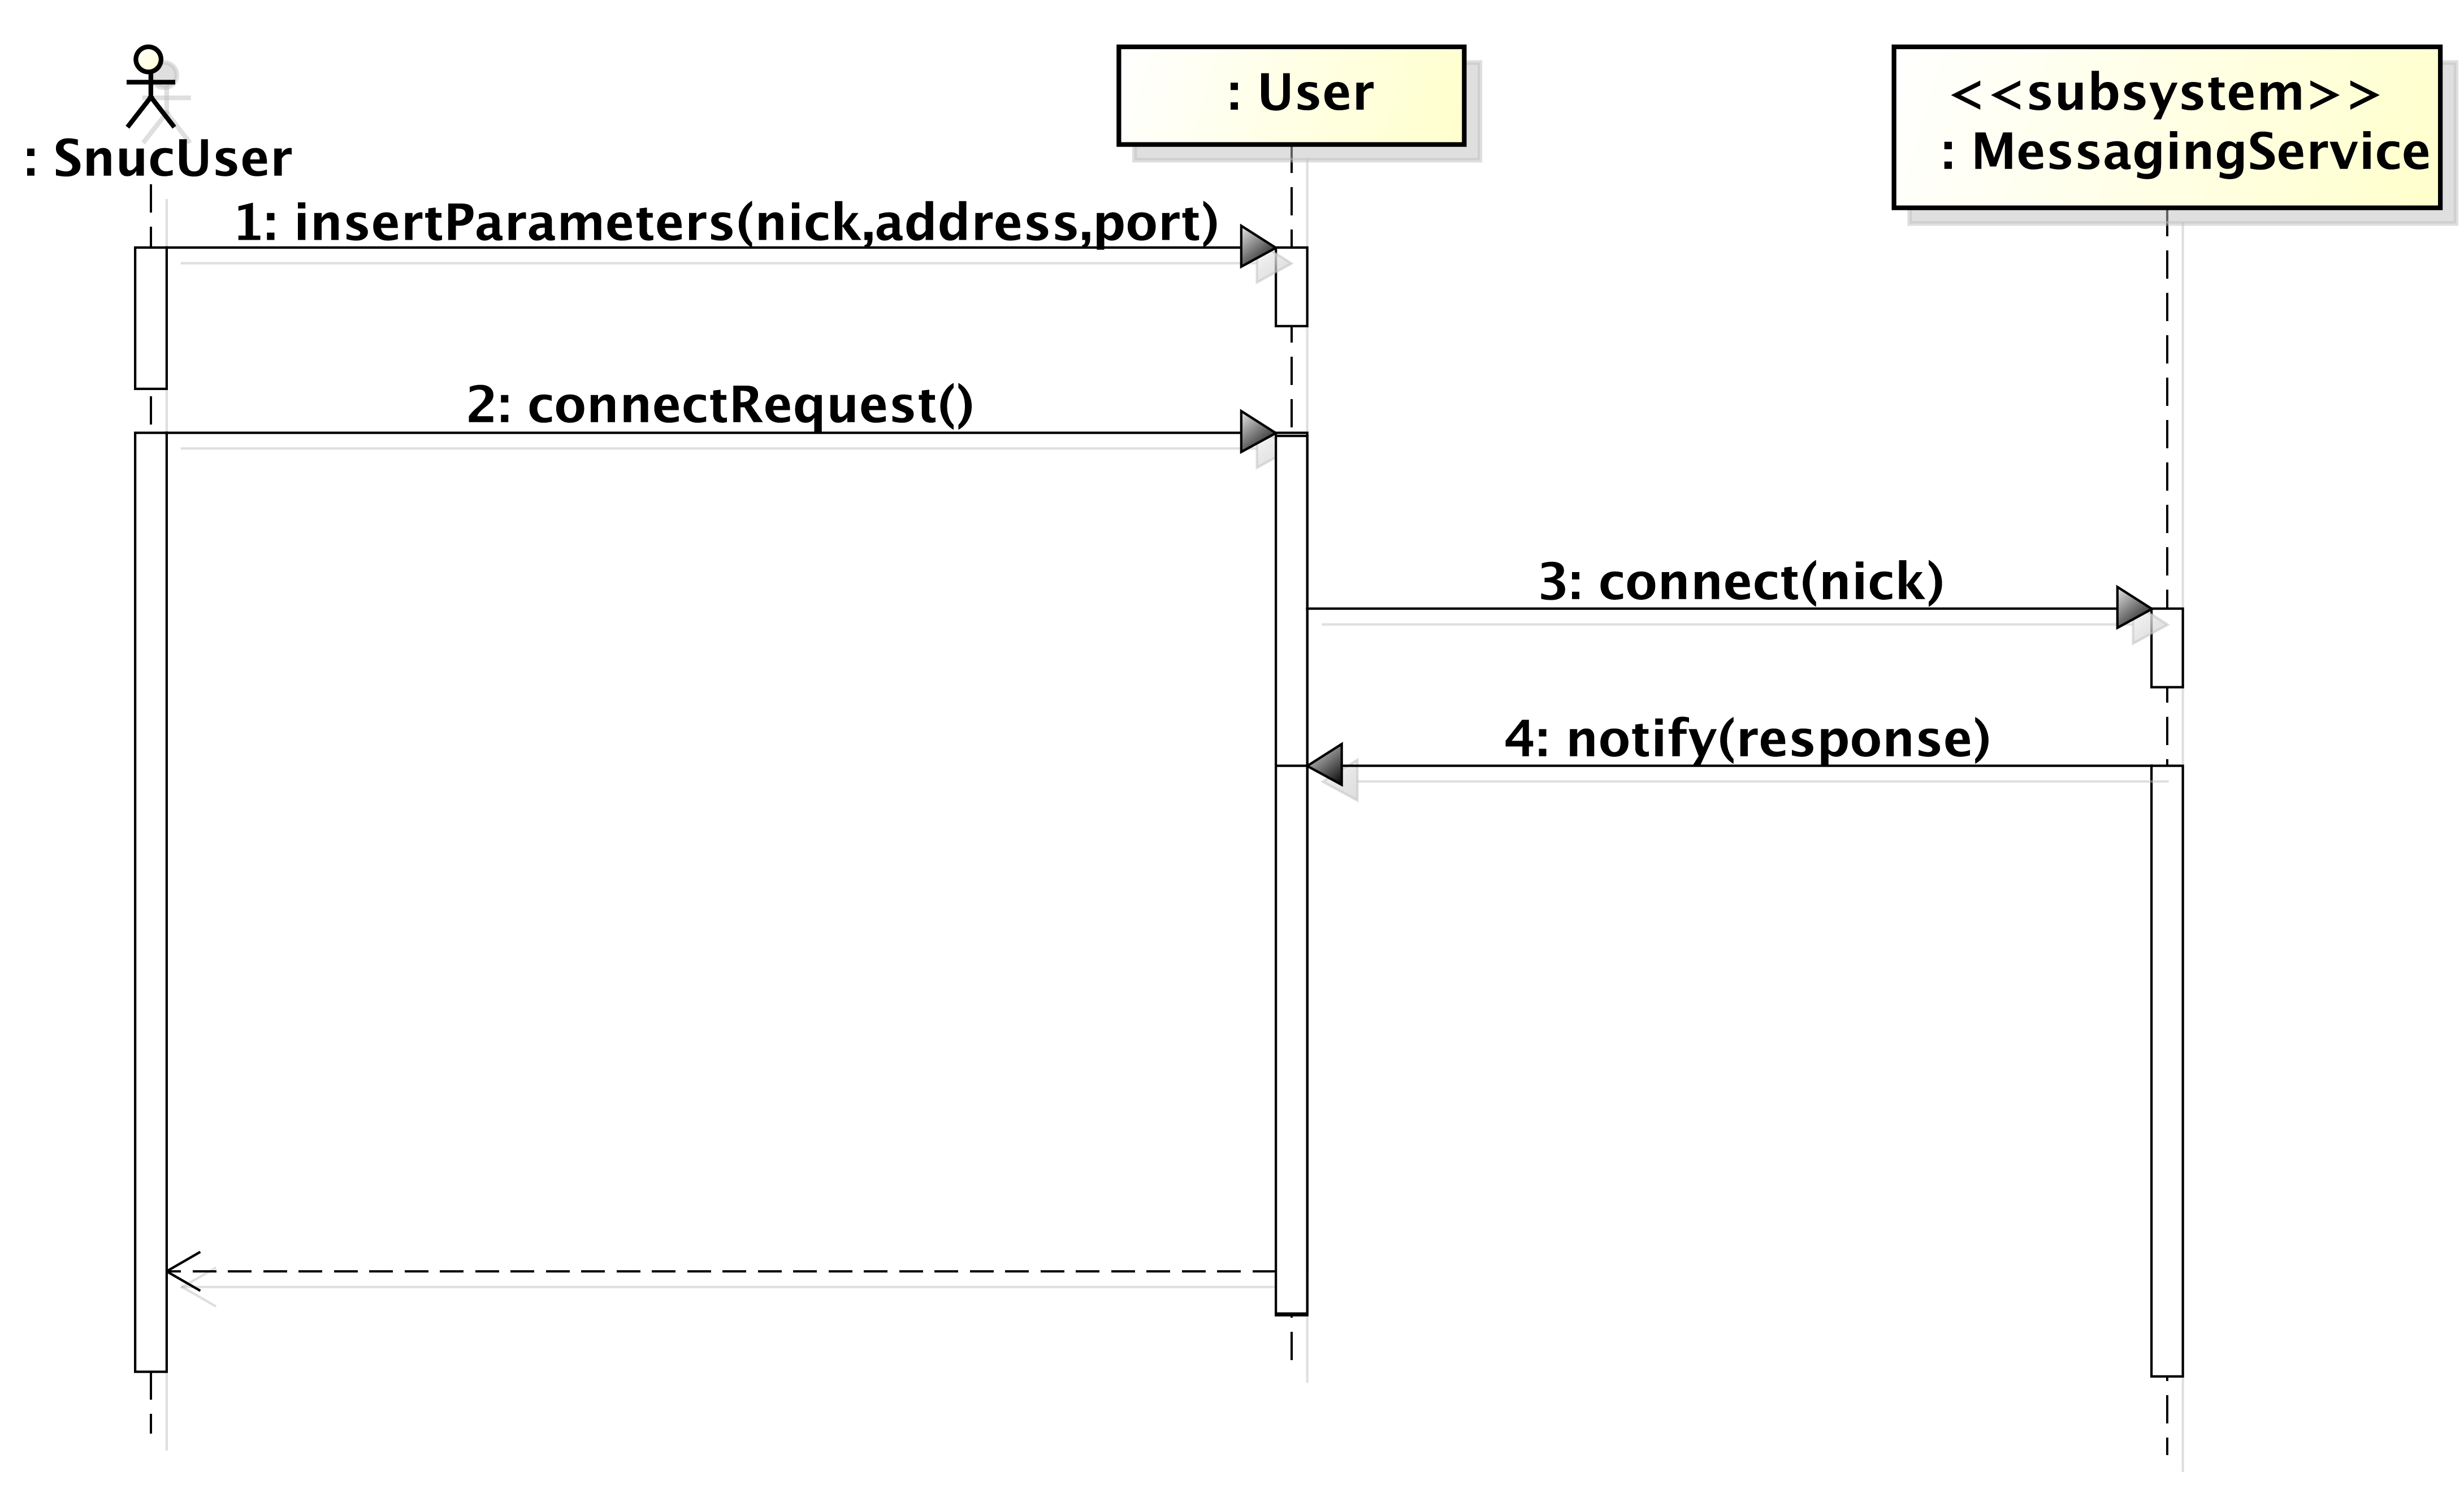
\includegraphics[scale=0.27]{image_astah/Iteration_1_DomainModel/UC1_RequestConnection_SSD.png}{\centering}
     \caption{UC1 - Diagramma di sequenza di sistema}
     \label{fig_UC1_RC_SSD} 
   \end{figure}
\end{frame}

\begin{frame}
 \frametitle{Iterazione 1: Analisi - UC1 contratti CO1/CO2}
  \begin{table}[!htbp]
   \caption {UC1 Contratto CO1 - connect}
    \label{table_CO1}
      \resizebox{\linewidth}{!}{%
       \begin{tabular}{|l|p{10cm}|}\hline
         Operazione & \textit{connect(nick: String)}  \\\hline 
         Riferimenti &  Caso d'uso: UC1\_RequestConnection \\\hline
         Pre-condizione & L'utente ha inserito correttamente i parametri di connessione (``address'' e ``port'') \\\hline 
         Post-condizione & L'utente è connesso al servizio di messaggistica e viene aggiunto nella lista degli utenti online \\\hline
      \end{tabular}}
   \end{table}
  \begin{table}[!htbp]
   \caption {UC1 Contratto CO2 - notify}
    \label{table_CO2}
      \resizebox{\linewidth}{!}{%
       \begin{tabular}{|l|p{10cm}|}\hline
         Operazione & \textit{notify(n: Notify)} \\\hline 
         Riferimenti &  Caso d'uso: UC1\_RequestConnection \\\hline
         Pre-condizione & L'utente è connesso al servizio di messaggistica \\\hline 
         Post-condizione & L'utente riceve la notifica \\\hline
      \end{tabular}}
   \end{table}

\end{frame}

\subsection{Iterazione 1: Analisi - UC2\_AccessRoom}
\begin{frame} [allowframebreaks] {Descrizione Analisi - UC2\_AccessRoom}
  In questa iterazione, del caso d’uso UC2 è di interesse lo scenario principale di successo.  Da esso è possibile identificare le seguenti classi concettuali: 
  \begin{itemize}
    \item \textbf{User}: rappresenta il generico utente, caratterizzato da un ``nickname'', connesso al servizio di messaggistica. \textit{Può richiedere la lista 
     delle stanze, ricevere notifiche dal sistema centrale. Interagisce con il MessagingSevice richiedendo la registrazione e l'ingresso in una specifica stanza}.
    \item \textbf{MessagingService}: rappresenta ed incapsula il servizio di messaggistica nel suo complesso. Mantiene una lista di utenti connessi a tale 
    sistema. \textit{Mantiene una lista di stanze e riceve tramite comandi richieste di ingresso da parte degli utenti}.
    \item \textbf{Message}: individua un generico messaggio scambiato tra utenti della chat o tra servizio di messaggistica e utente. È costituito da un ``content'' 
          (contenuto del messaggio), da una ``date'' (rappresenta la data) e dal ``sender'' (mittente).
    \item \textbf{Notify}: è una specializzazione del tipo Message ed è caratterizzata da un typeNotify che serve a distinguere il tipo di notifica (ad es. 
          CONNECTIO\_ACCEPT nel caso in cui la connessione è stata stabilita correttamente, \textit{BAD\_COMMAND nel caso in cui il comando inviato dall'User non 
          sia riconosciuto dal Server)}.
    \item \textit{\textbf{PublicNotify}: è una specializzazione di Notify e questo tipo di notifica viene ricevuta da tutti gli utenti registrati alla relativa 
          stanza. Un esempio di PublicNotify è la notifica caratterizzata dal seguente typeNotify: UPDATE\_LIST\_USERS, grazie alla quale viene 
          aggiornata la lista degli utenti registrati nella relativa stanza}.
   \item  \textit{\textbf{Commad}: è una specializzazione di Message e rappresenta il comando che viene inviato dall'User e ricevuto ed interpretato dal            
          MessagingService (es. /join '\#Medical' richiesta da parte dell'utente a registrarsi alla stanza Medical)}.        
    \item \textit{\textbf{Room}: è caratterizzata da un nome. Ciascuna istanza individua una specifica stanza nella chat}.
    \item \textit{\textbf{Register}: mantiene un riferimento all’insieme di partecipanti che in un certo istante sono presenti nella stanza}.
   \end{itemize}
\end{frame}

\begin{frame} {Iterazione 1: Analisi - UC2\_AccessRoom}
   \begin{figure}
     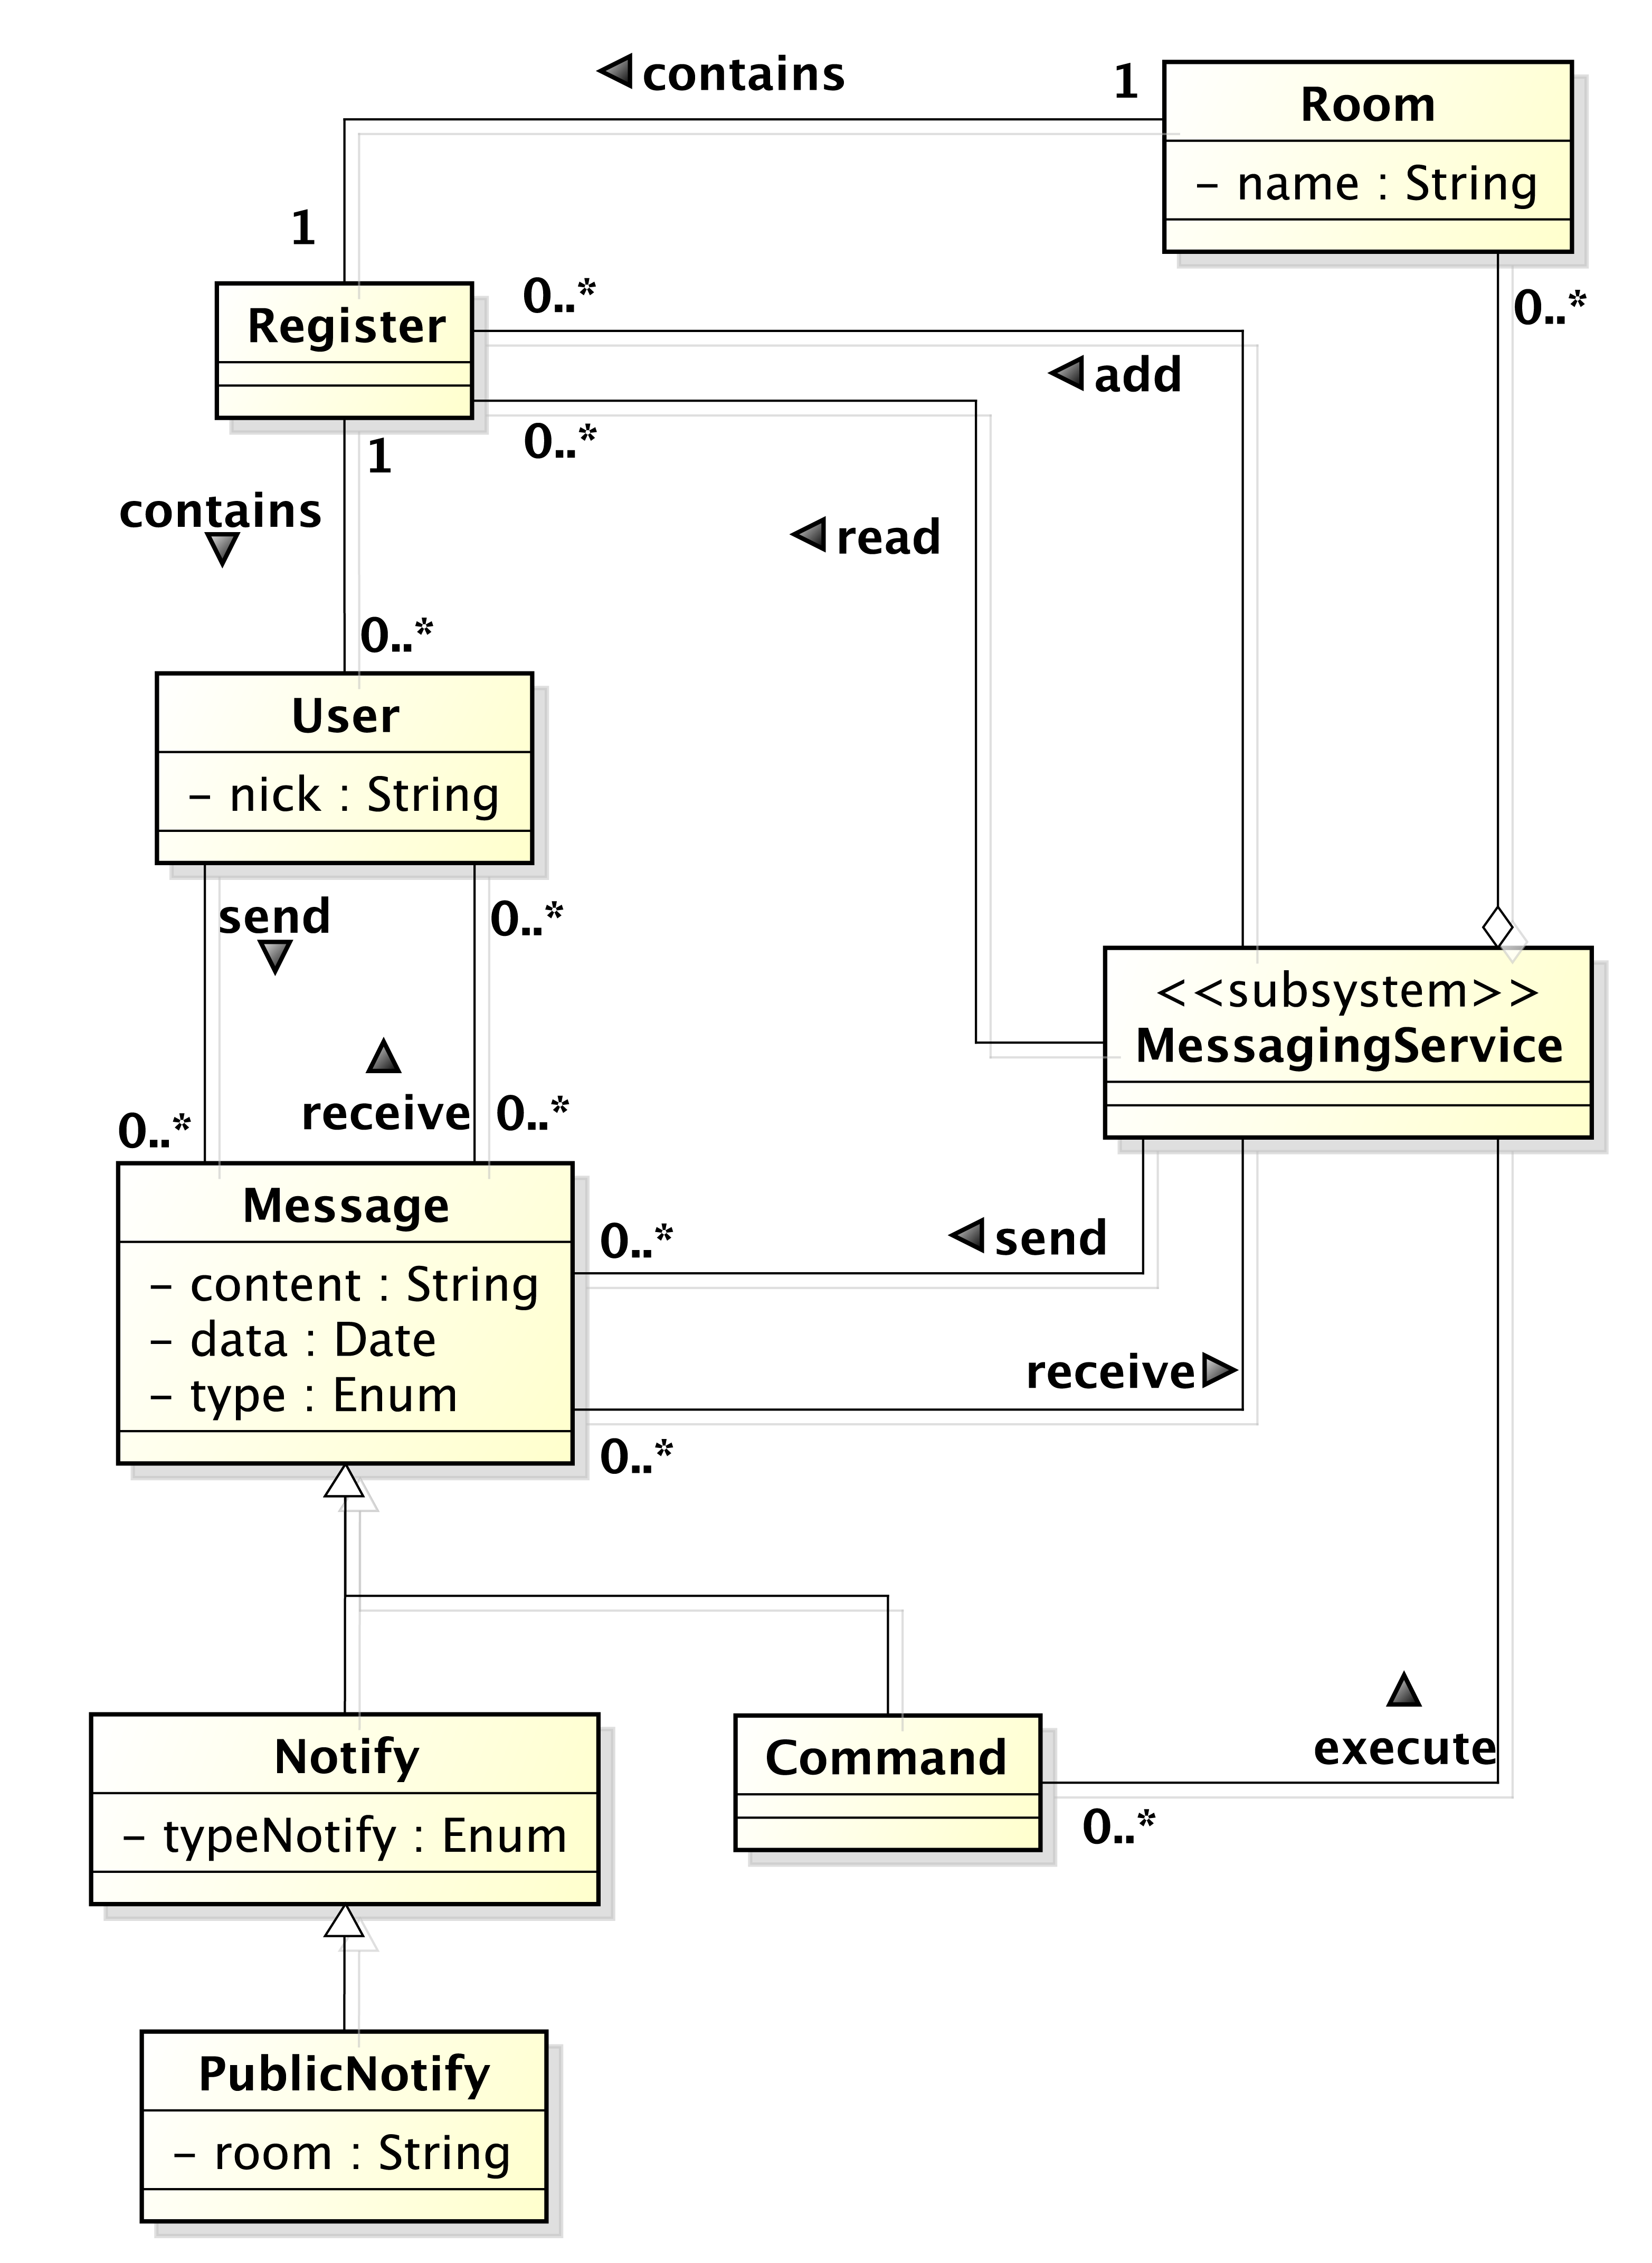
\includegraphics[scale=0.165]{image_astah/Iteration_1_DomainModel/UC2_AccessRoom_DM.png}{\centering}
     \caption{UC2 - Modello di dominio}
     \label{fig_UC2_AR_DM} 
   \end{figure}
\end{frame}

\begin{frame} {Iterazione 1: Analisi - UC2\_AccessRoom}
   \begin{figure}
     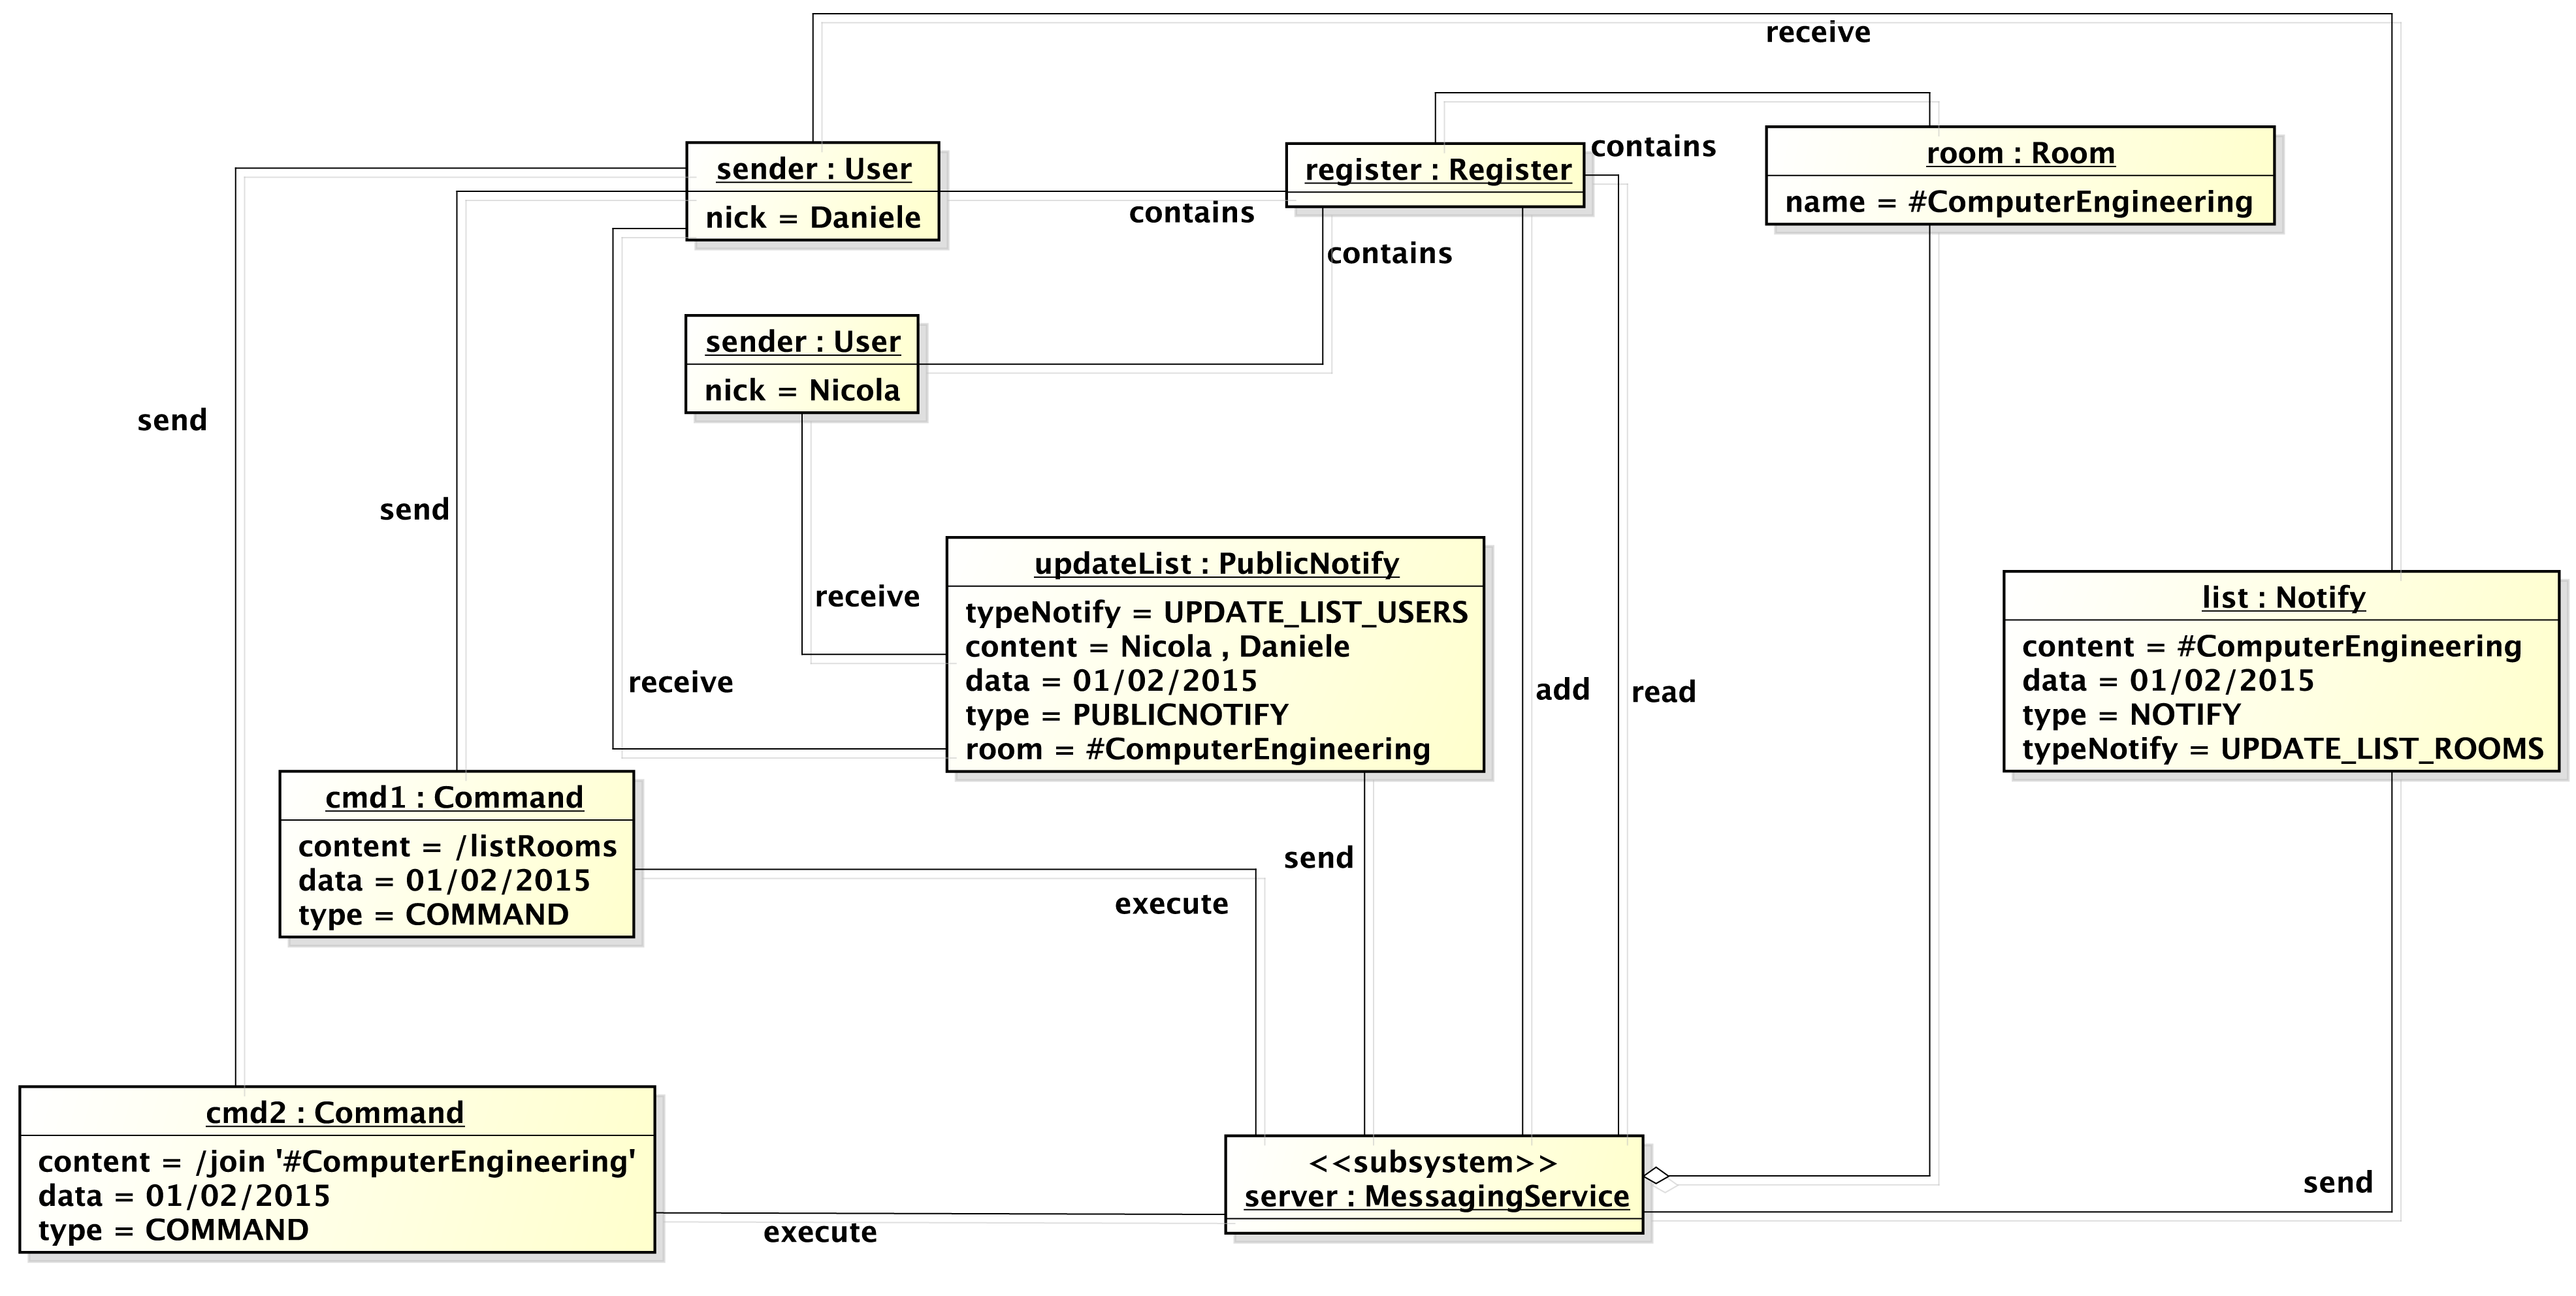
\includegraphics[scale=0.17]{image_astah/Iteration_1_DomainModel/UC2_AccessRoom_OM}{\centering}
     \caption{UC2 - Oggetti di dominio}
     \label{fig_UC2_AR_OM} 
   \end{figure}
\end{frame}

\begin{frame} {Iterazione 1: Analisi - UC2\_AccessRoom}
   \begin{figure}
     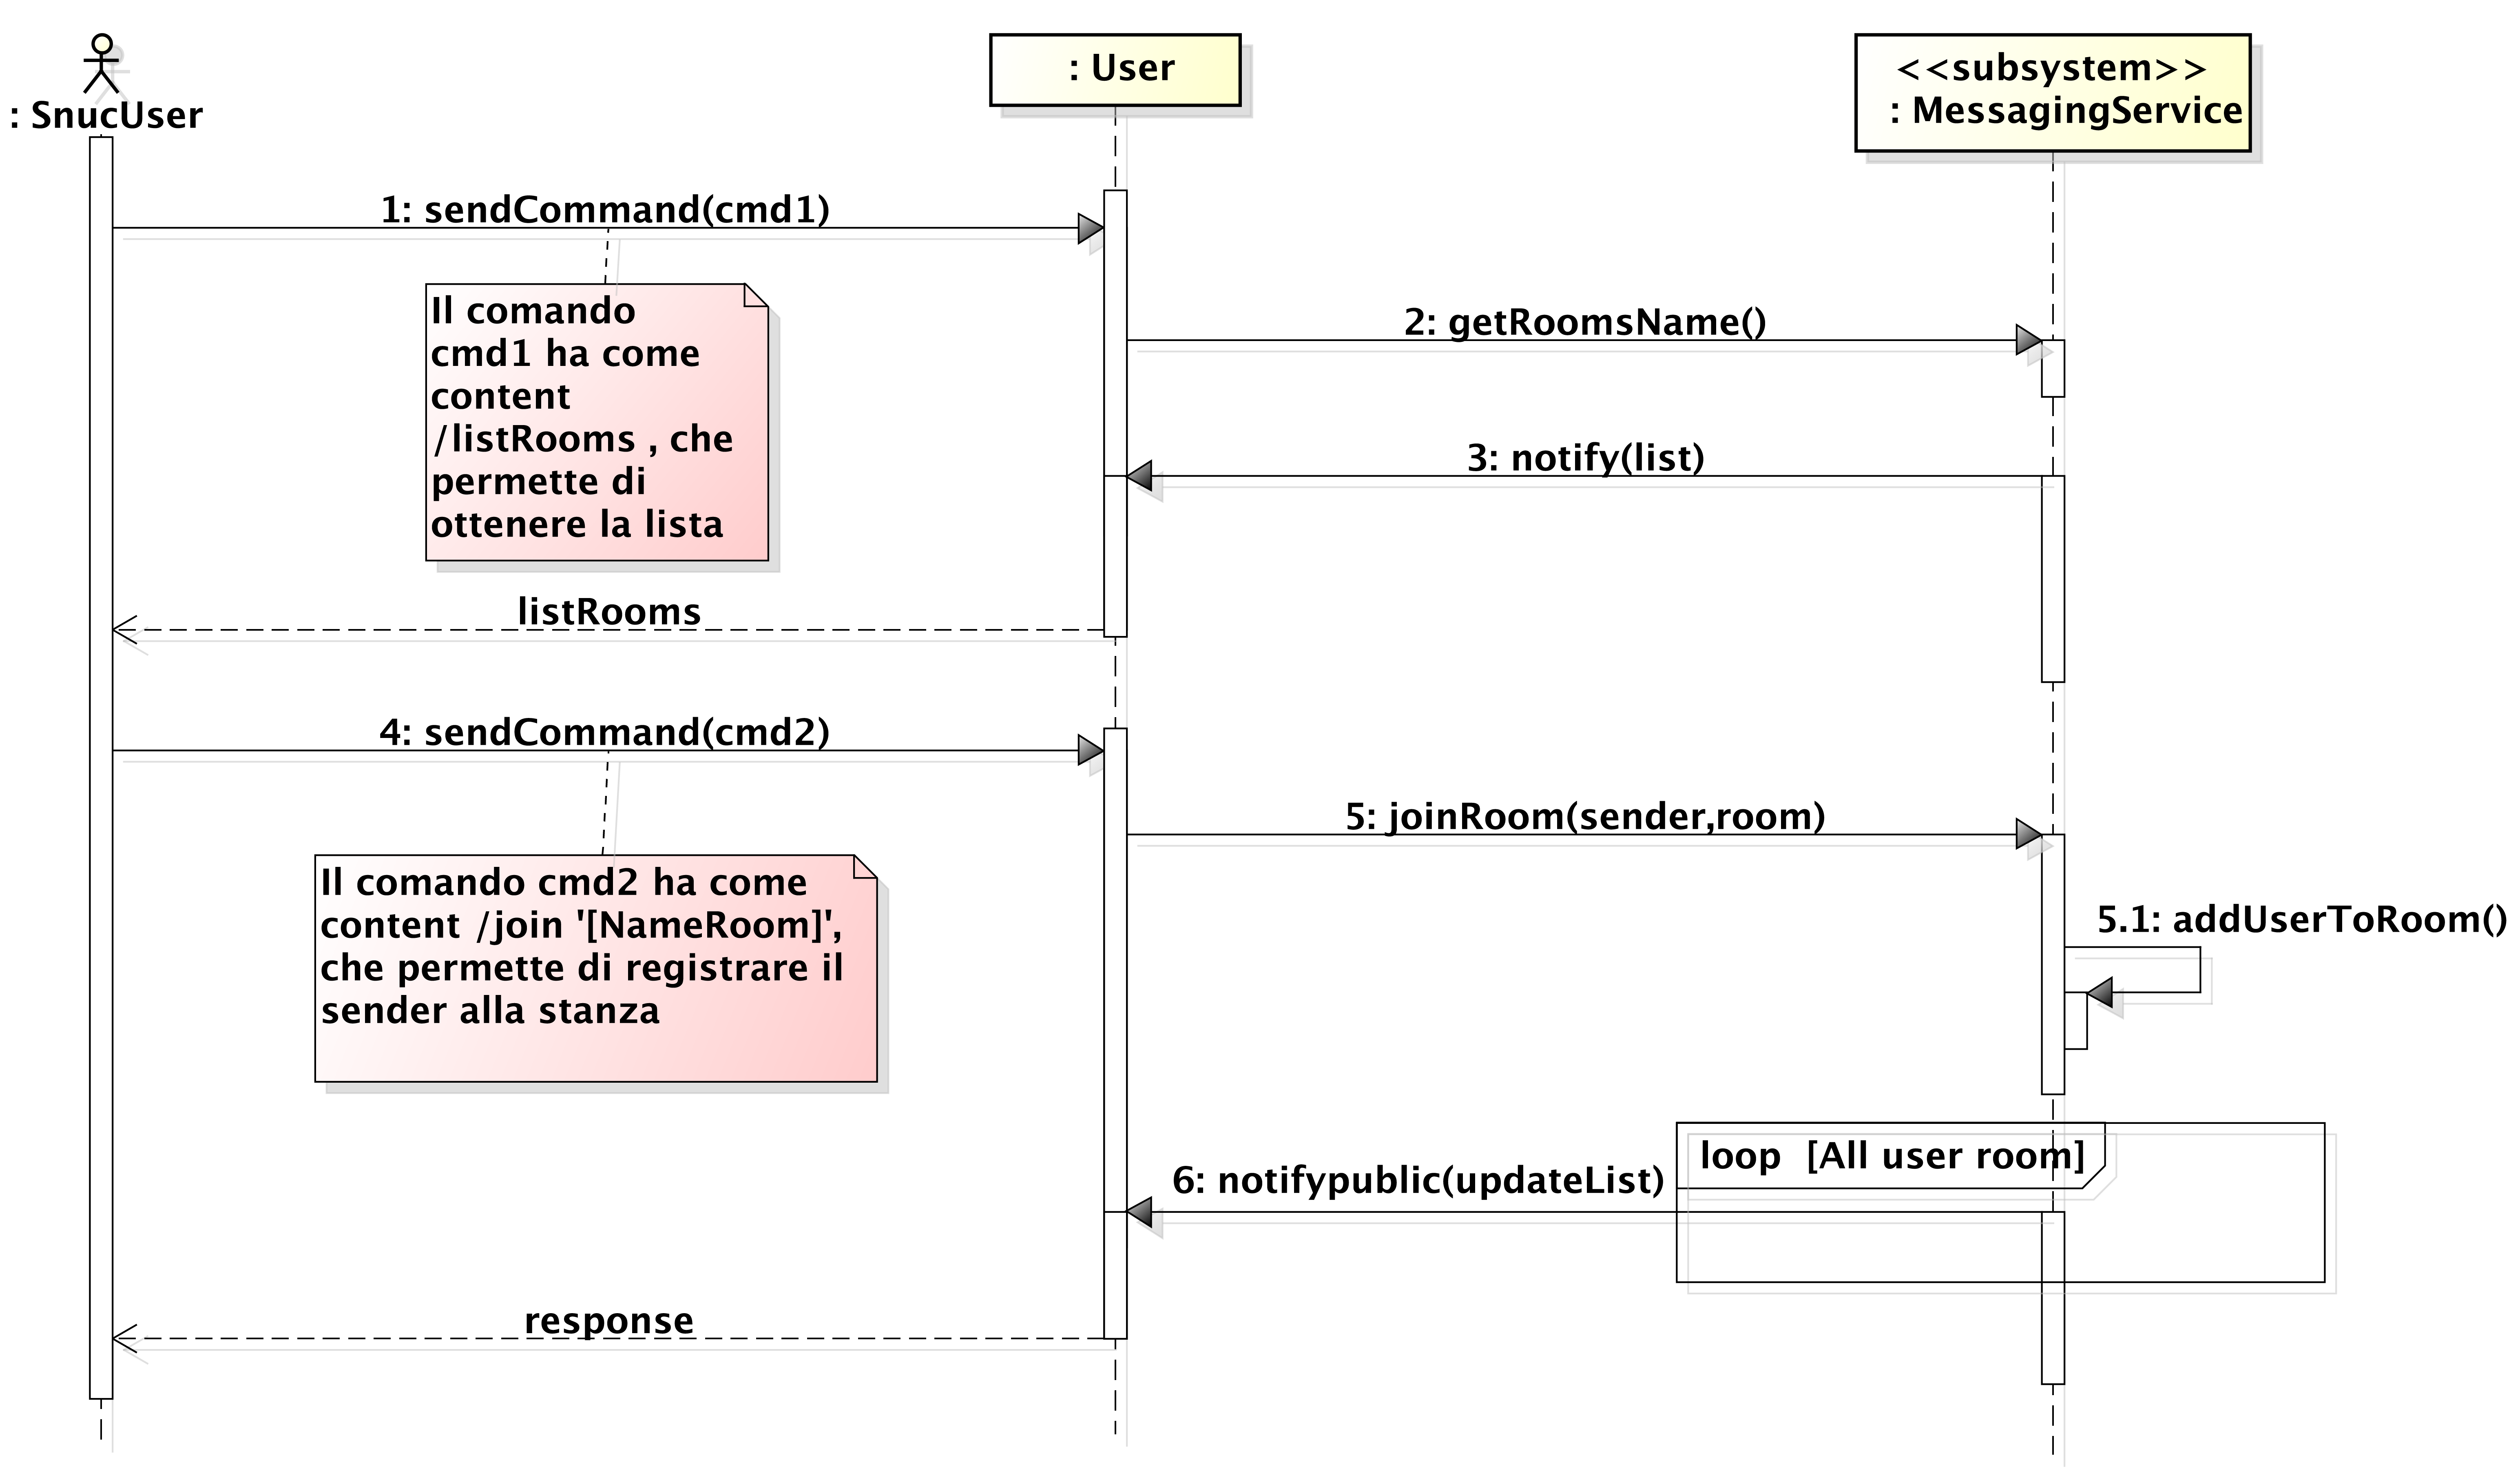
\includegraphics[scale=0.20]{image_astah/Iteration_1_DomainModel/UC2_AccessRoom_SSD.png}{\centering}
     \caption{UC2 - Diagramma di sequenza di sistema}
     \label{fig_UC2_AR_SSD} 
   \end{figure}
\end{frame}

\begin{frame} [allowframebreaks]
 \frametitle{Iterazione 1: Analisi - UC2 contratti CO3/CO4}
  \begin{table}[!htbp]
   \caption {UC2 Contratto CO3 - joinRoom}
    \label{table_CO3}
      \resizebox{\linewidth}{!}{%
       \begin{tabular}{|l|p{10cm}|}\hline
         Operazione & \textit{joinRoom(sender: String, room: String)} \\\hline 
         Riferimenti & Caso d'uso: UC2\_AccessRoom \\\hline
         Pre-condizione & 
         \begin{itemize}
          \item L'utente è connesso al servizio di messaggistica
          \item L'utente ha inserito il comando relativo alla registrazione nella stanza       
         \end{itemize} \\\hline 
         Post-condizione & Il server interpreta il comando ed inserirà l'utente nella lista degli utenti registrati nella stanza  \\\hline
      \end{tabular}}
   \end{table}
  \begin{table}[!htbp]
   \caption {UC2 Contratto CO4 - notifypublic}
    \label{table_CO4}
      \resizebox{\linewidth}{!}{%
       \begin{tabular}{|l|p{10cm}|}\hline
         Operazione & \textit{notifypublic(n: PublicNotify)} \\\hline 
         Riferimenti & Caso d'uso: UC1\_RequestConnection \\\hline
         Pre-condizione & Registrazione utente tra gli utenti della stanza \\\hline 
         Post-condizione & Tutti gli utenti registrati nella stanza ricevono la notifica pubblica relativa all'aggiornamento della lista degli utenti  \\\hline
      \end{tabular}}
   \end{table}


\end{frame}

%ITERAZIONE 1 PROGETTAZIONE 

\subsection{Iterazione 1: Progettazione}
\begin{frame} {Descrizione Iterazione 1: Progettazione}
 \emph{INSERIRE DESCRIZIONE}
\end{frame}

\subsection{Iterazione 1: Progettazione - Class Diagram UC1 e UC2}
\begin{frame} {Iterazione 1: Progettazione - Class Diagram Common UC1 e UC2}
   \begin{figure}
     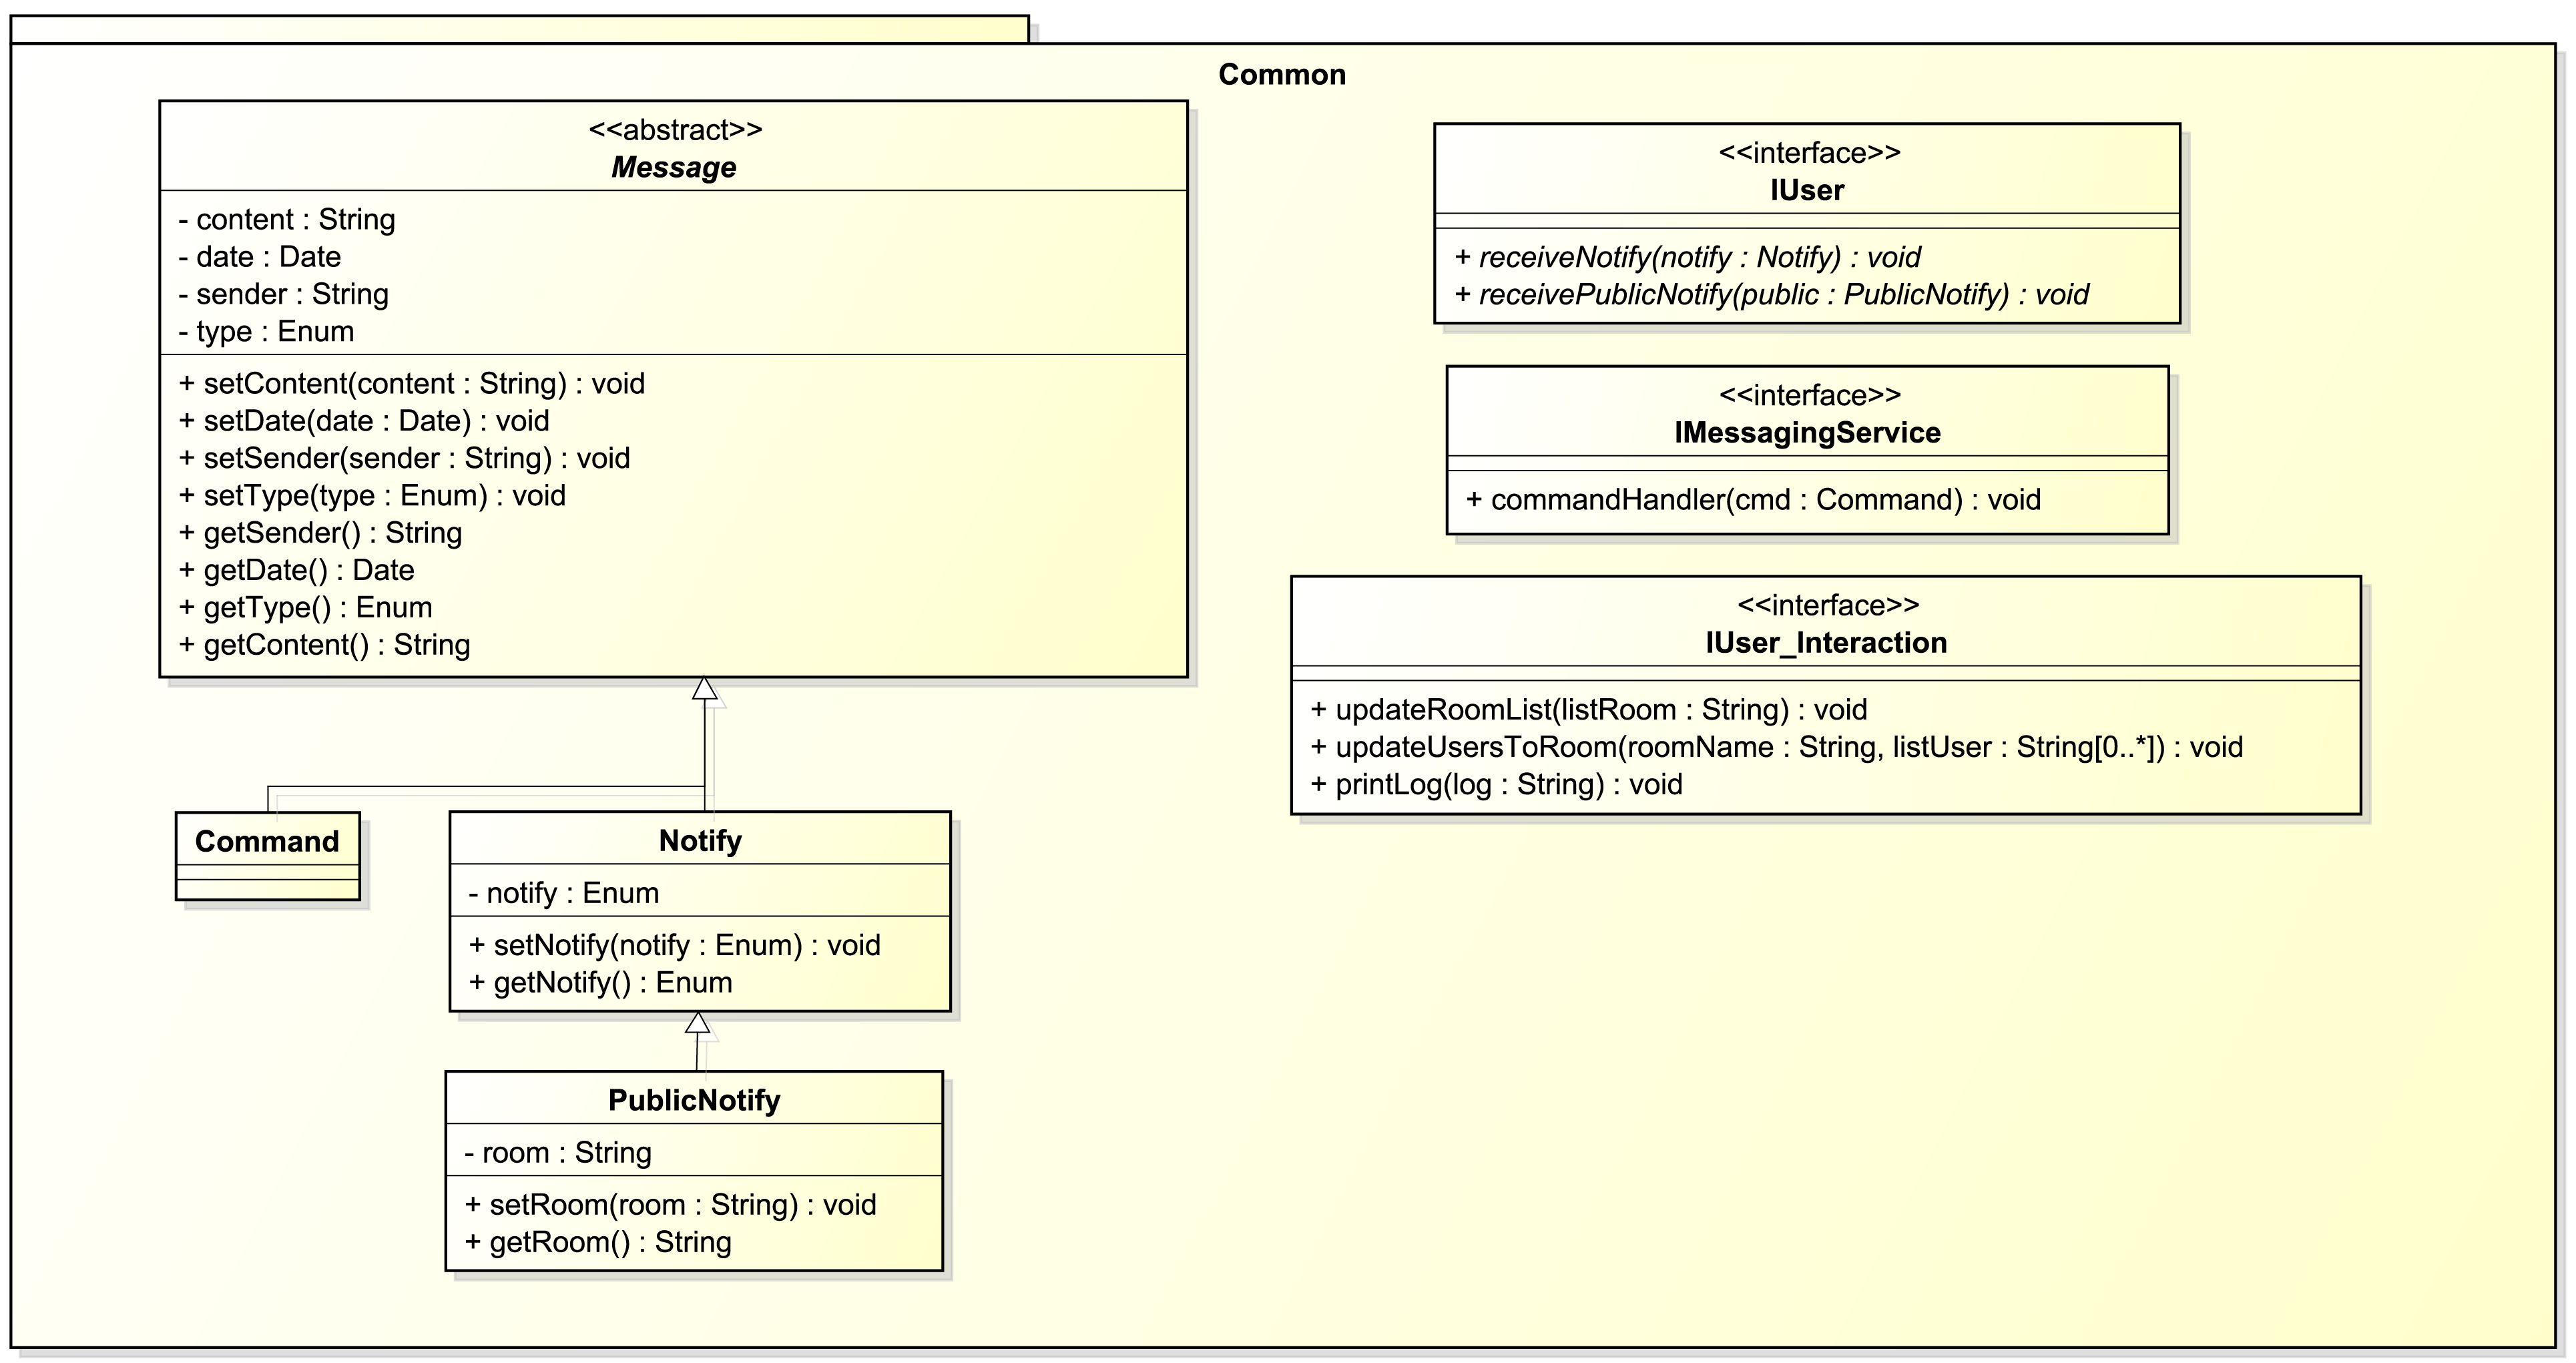
\includegraphics[scale=0.18]{image_astah/Iteration_1_DesignModel/ClassDiagramCommon.png}{\centering}
     \caption{DCD - Diagramma delle Classi: Package Common }
     \label{fig_UC1_UC2_DCD_1} 
   \end{figure}
\end{frame}

\begin{frame} {Iterazione 1: Progettazione - Class Diagram Snuc Server UC1 e UC2}
   \begin{figure}
     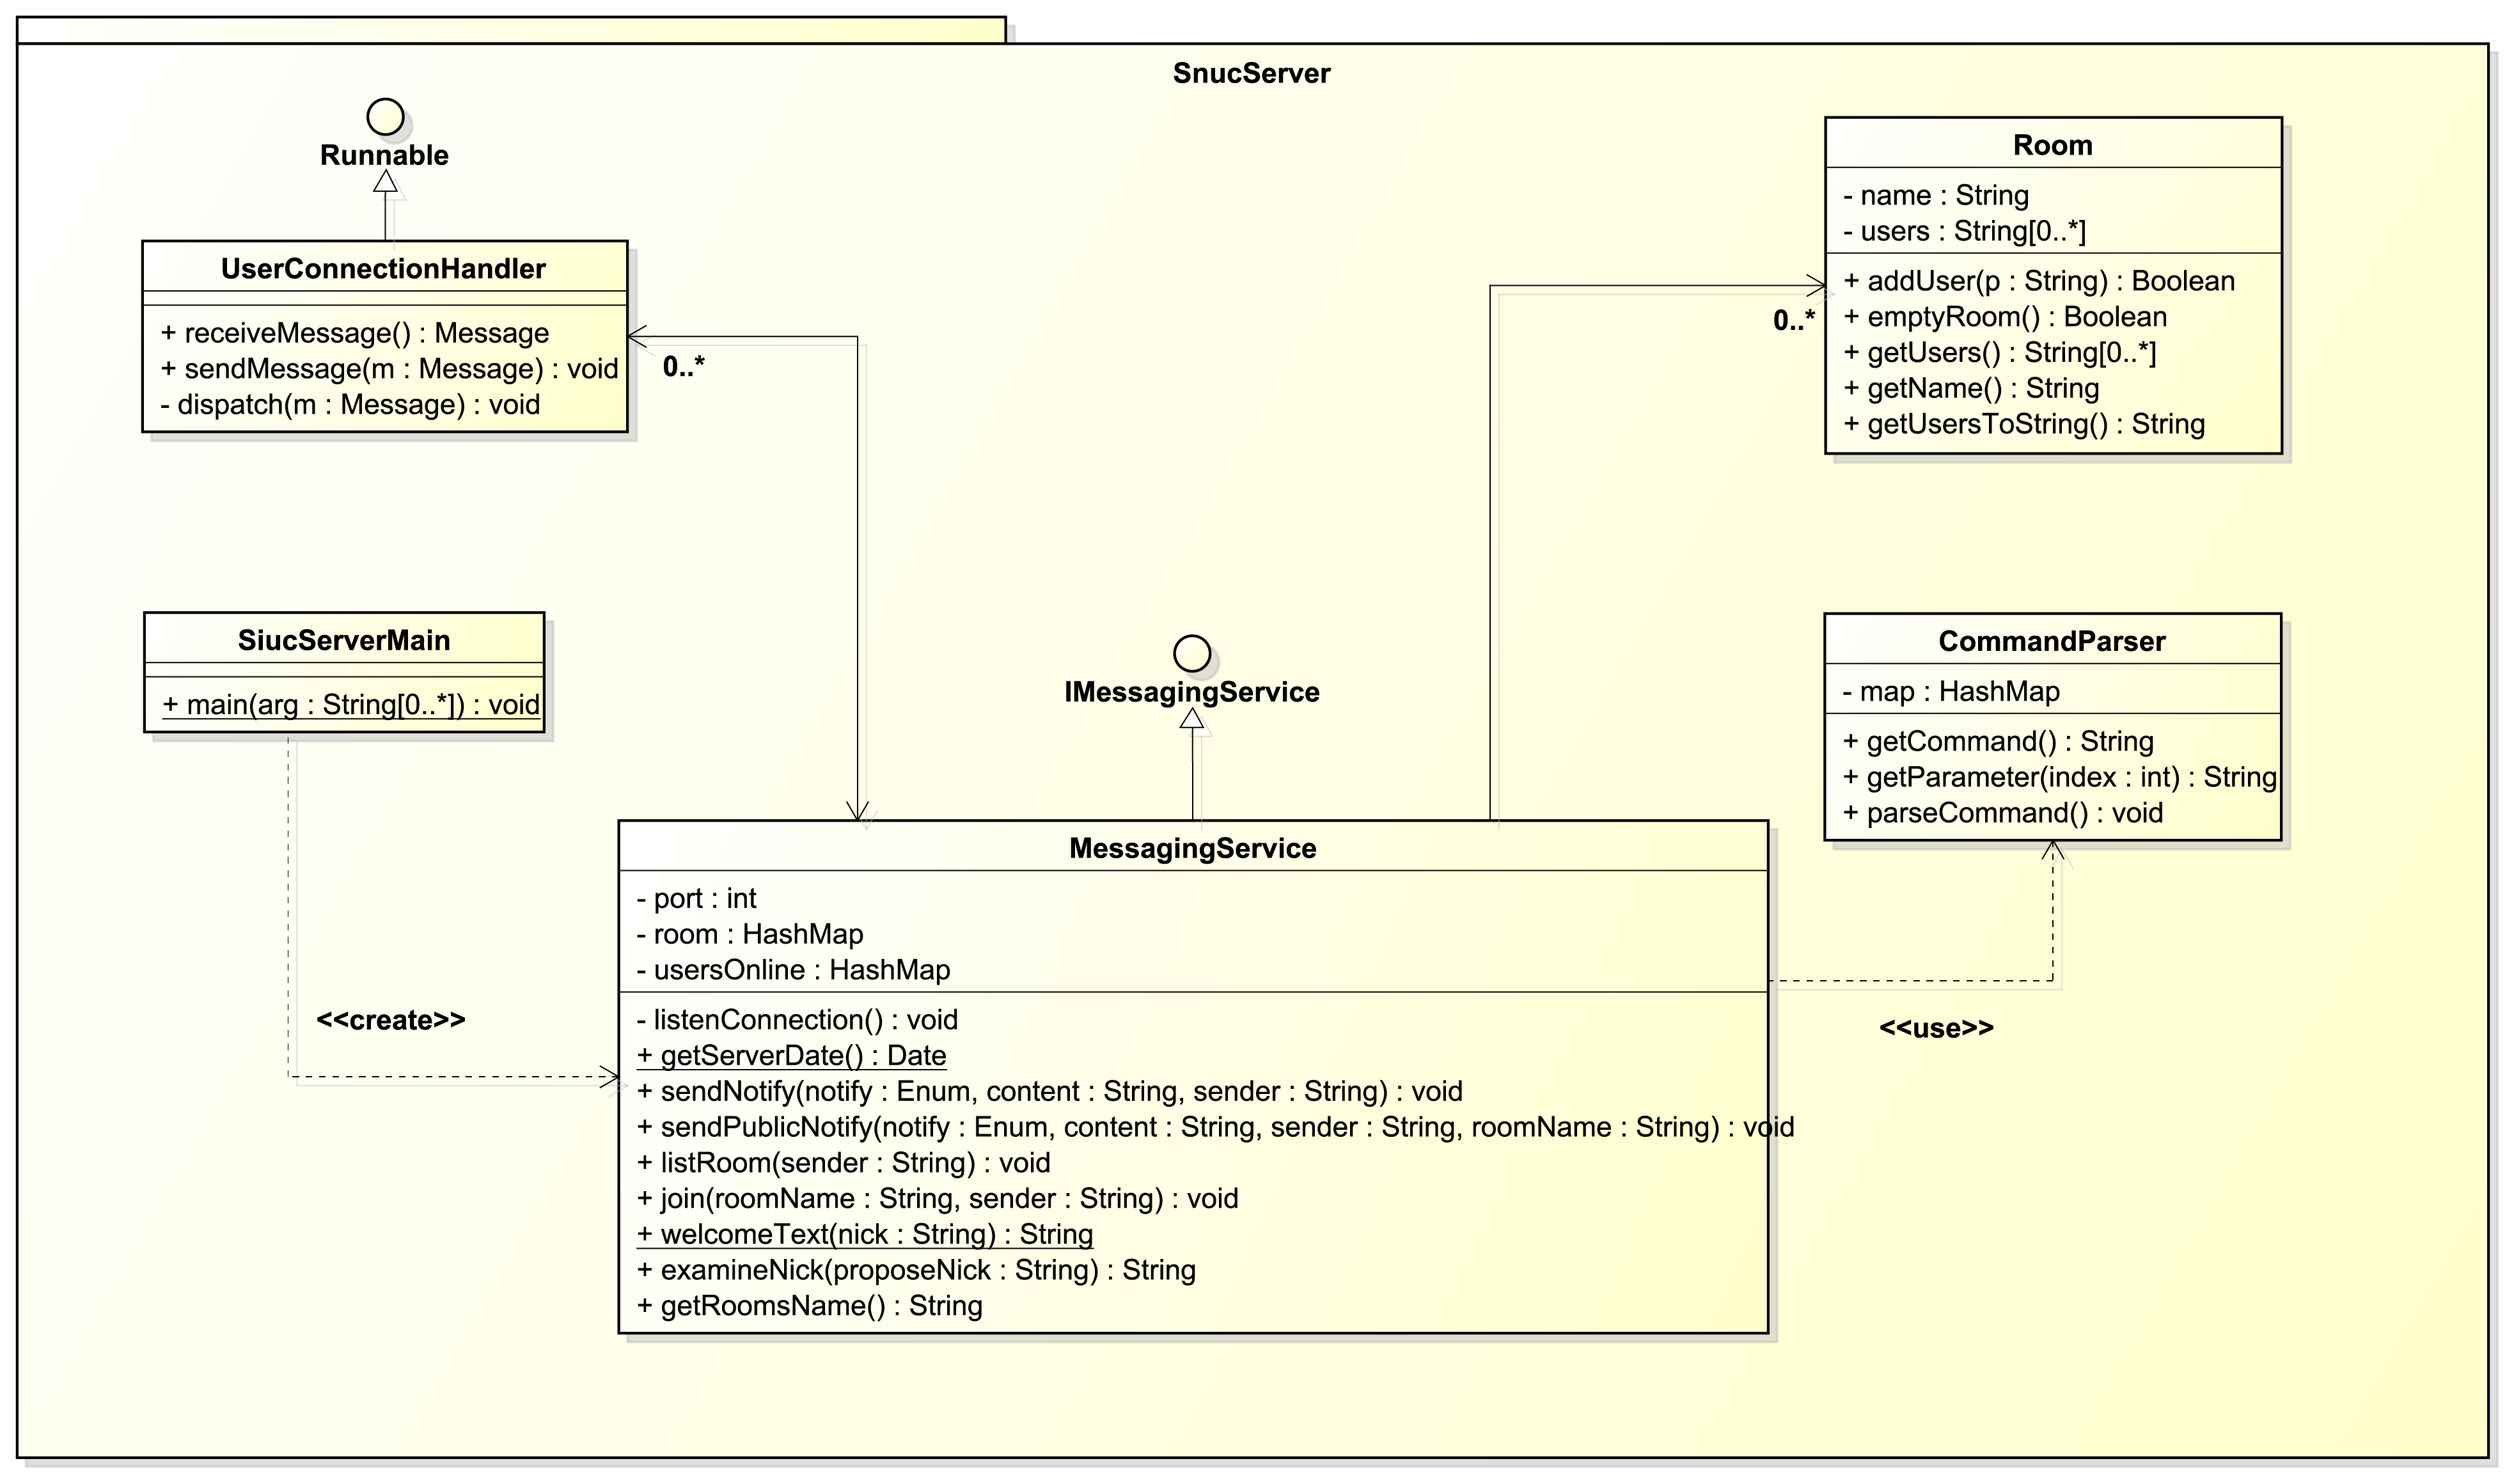
\includegraphics[scale=0.156]{image_astah/Iteration_1_DesignModel/ClassDiagramSnucServer.png}{\centering}
     \caption{DCD - Diagramma delle Classi: Package Snuc Server }
     \label{fig_UC1_UC2_DCD_2} 
   \end{figure}
\end{frame}

\begin{frame} {Iterazione 1: Progettazione - Class Diagram Snuc UC1 e UC2}
   \begin{figure}
     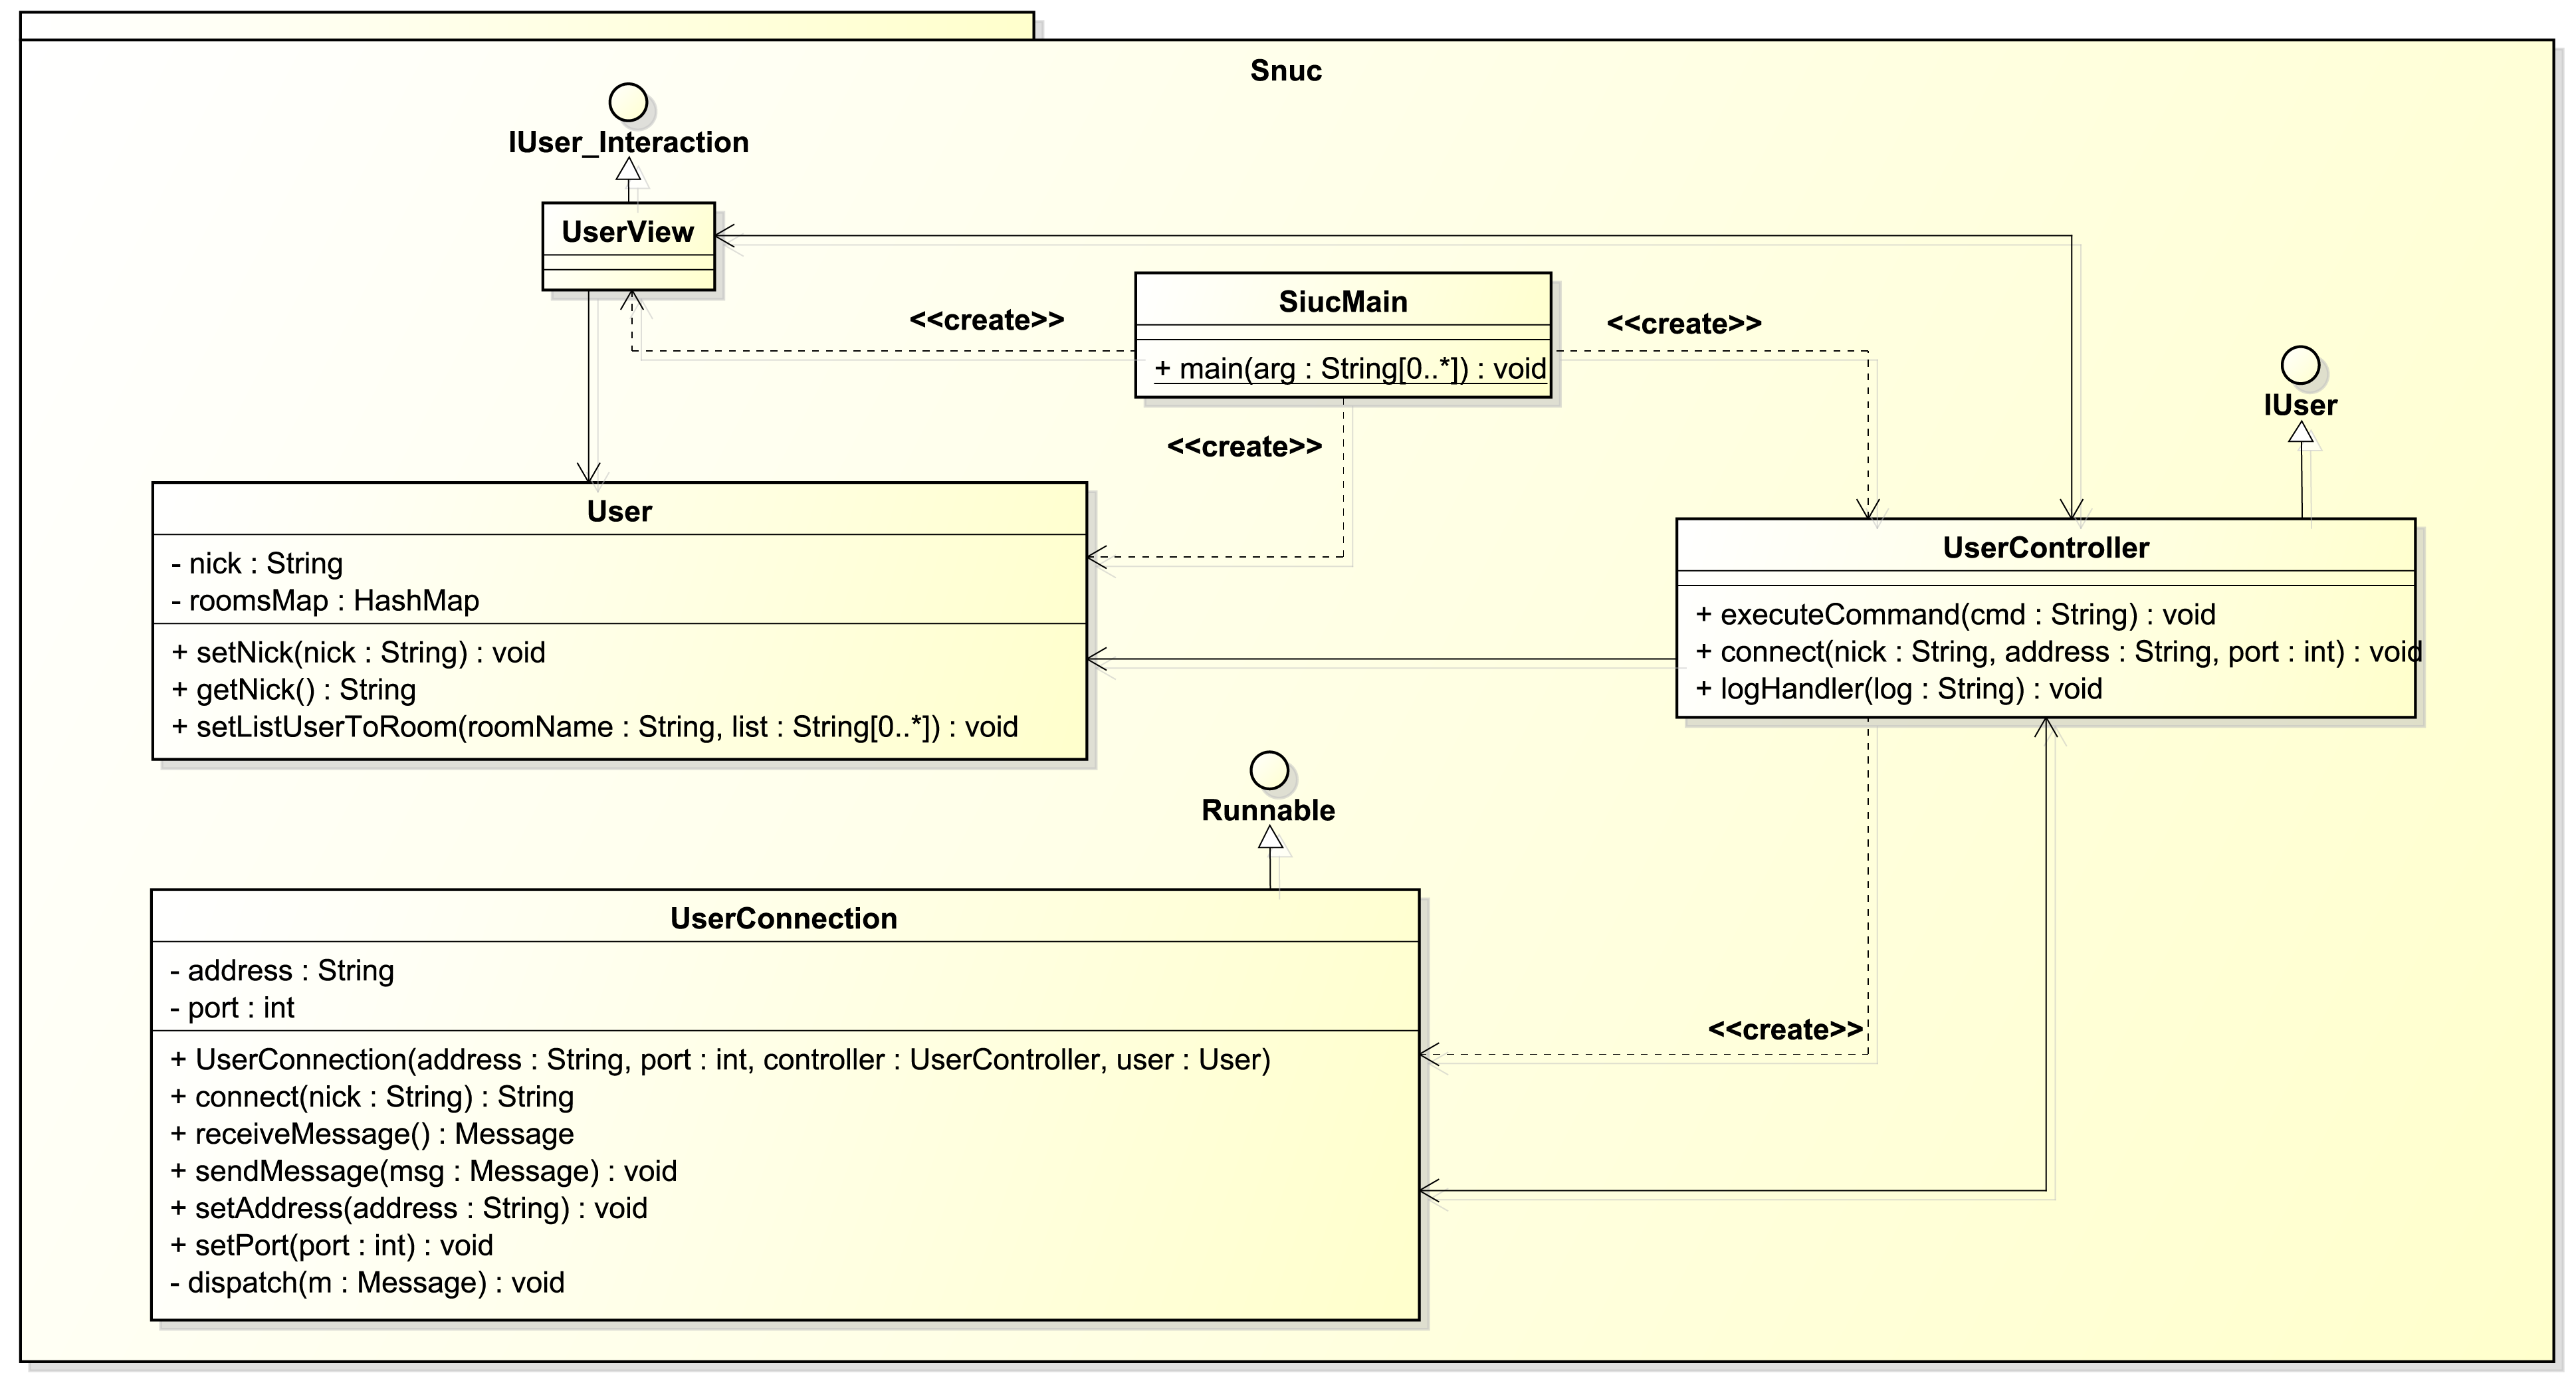
\includegraphics[scale=0.17]{image_astah/Iteration_1_DesignModel/ClassDiagramSnuc.png}{\centering}
     \caption{DCD - Diagramma delle Classi: Package Snuc }
     \label{fig_UC1_UC2_DCD_3} 
   \end{figure}
\end{frame}

\subsection{Iterazione 1: Progettazione - SSD  UC1\_RequestConnection}
\begin{frame} {Iterazione 1: Progettazione, UC1\_RequestConnection}
   \begin{figure}
     %\hypersetup{linkbordercolor={0 0.5 0.1}}
     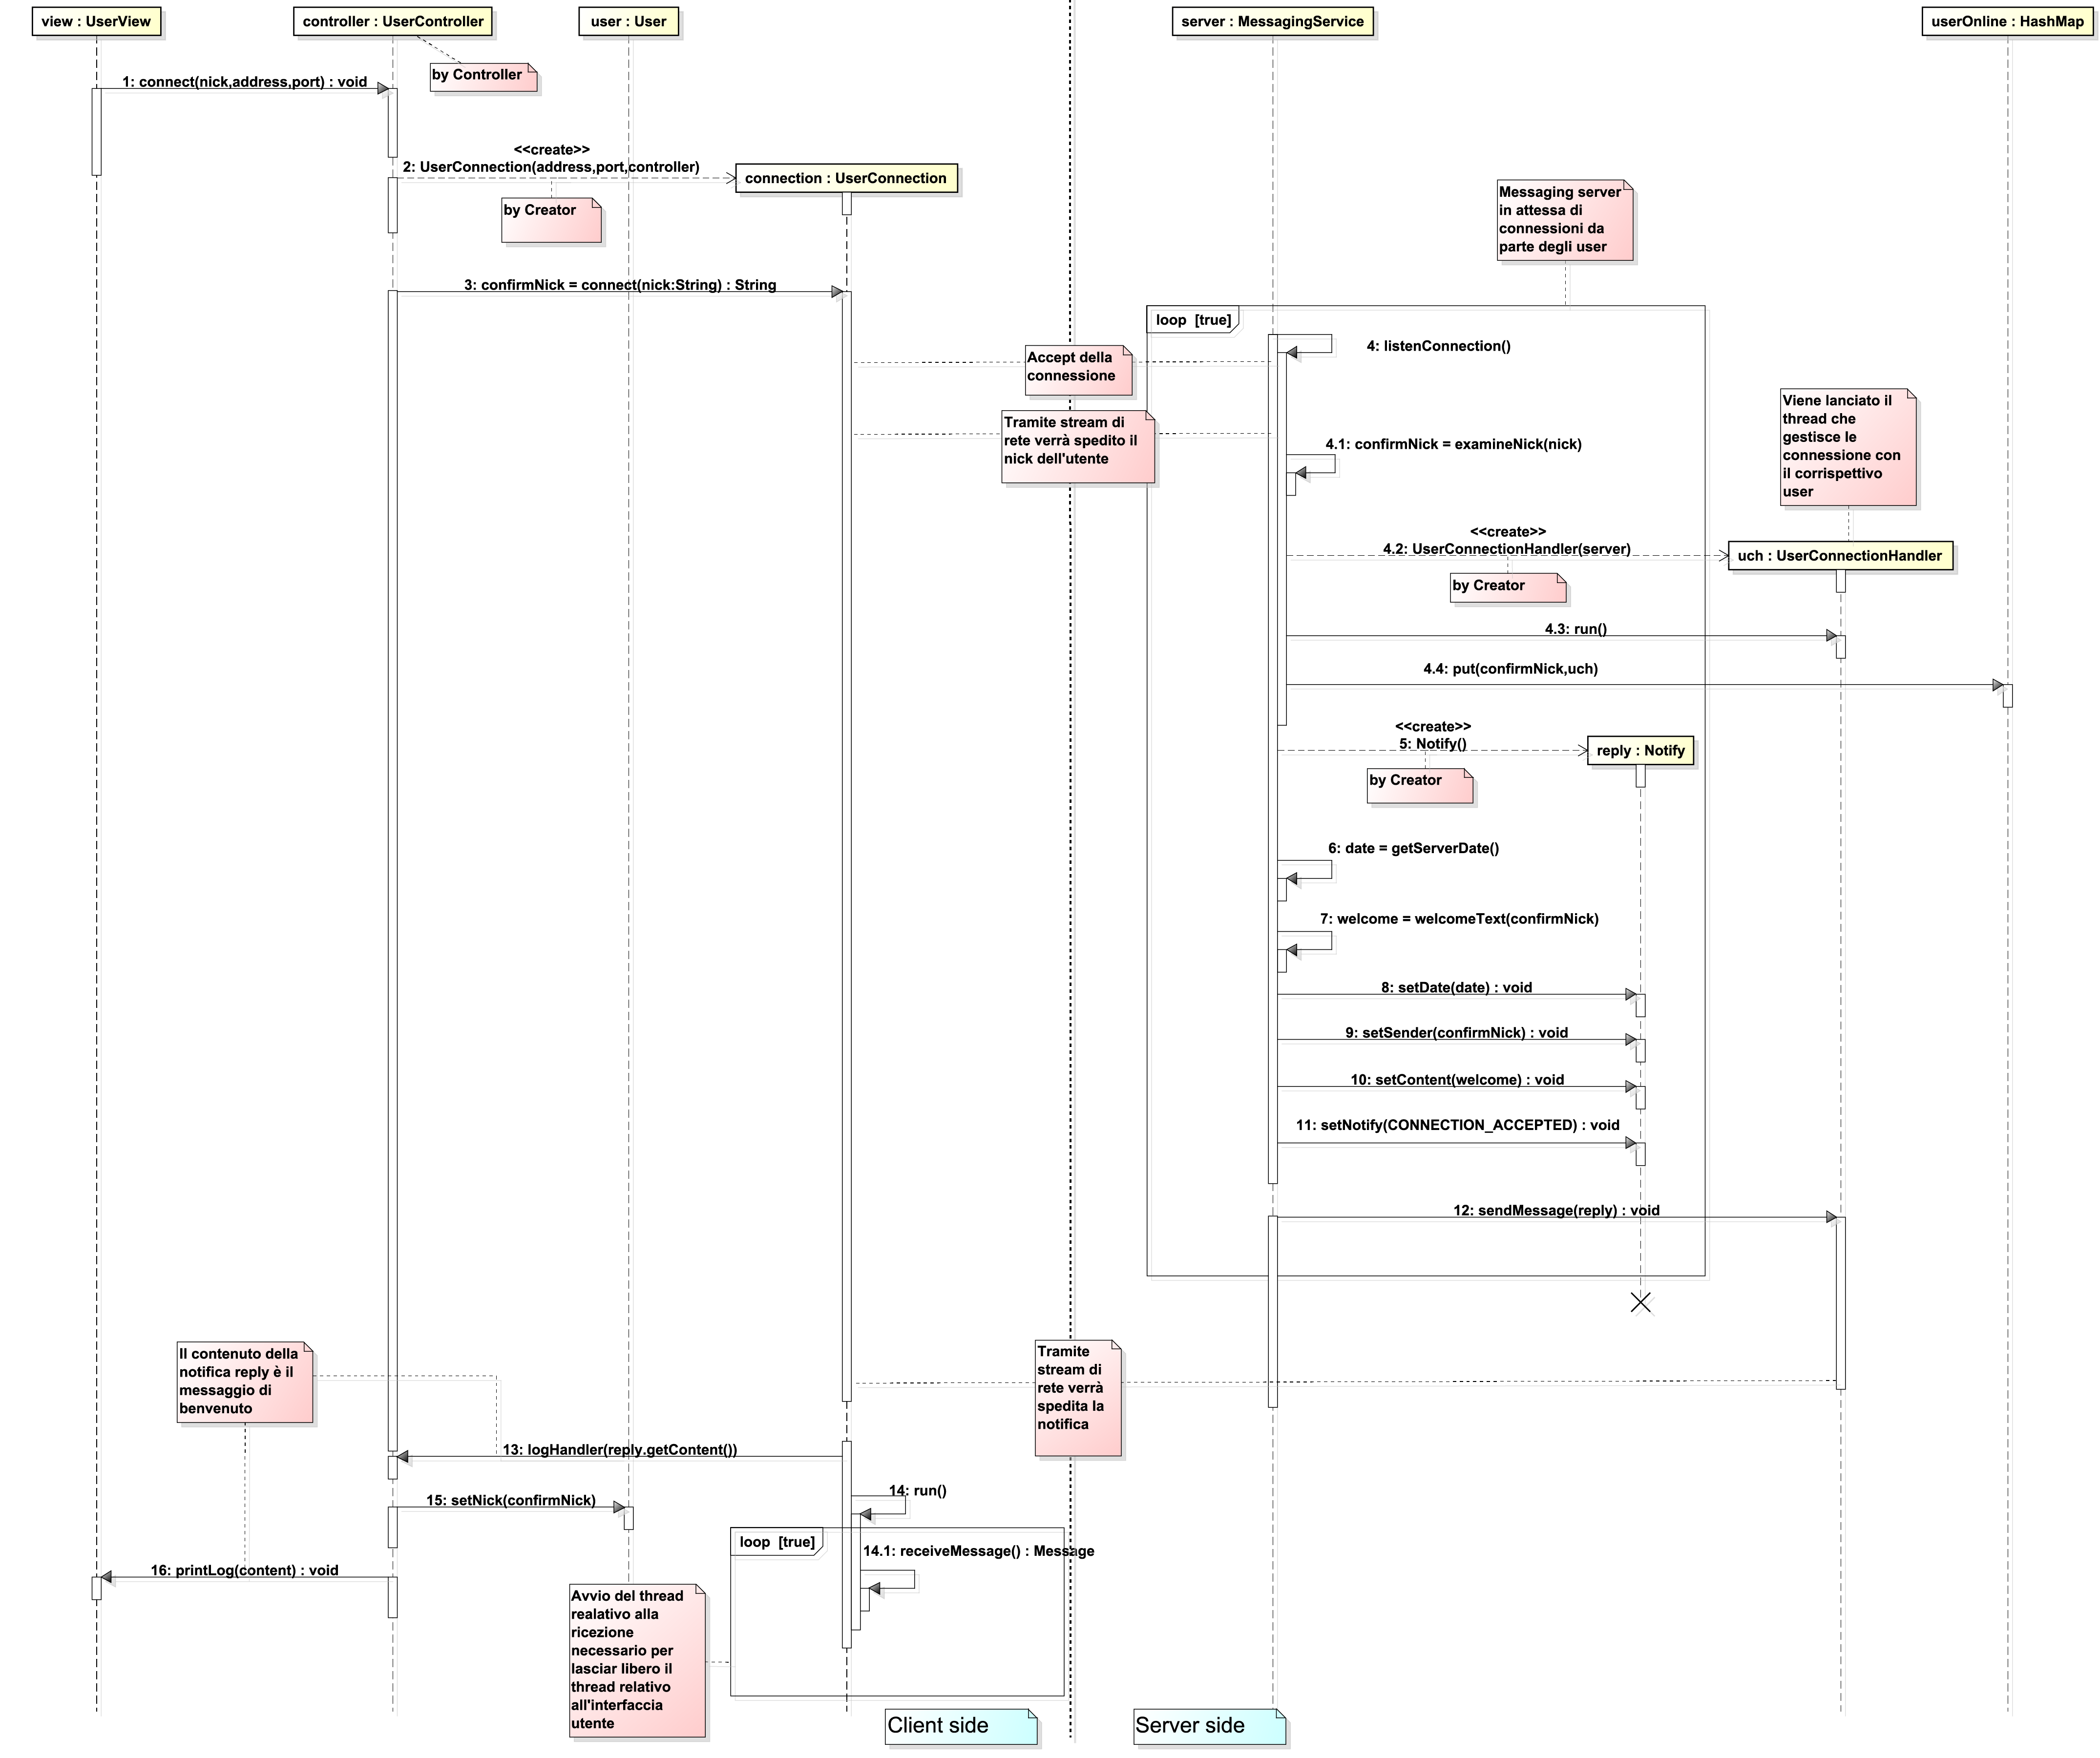
\includegraphics[scale=0.065]{image_astah/Iteration_1_DesignModel/UC1_RequestConnection_SSD_3_4_connect.png}{\centering}
     \caption{SSD - OP1-4: connect(nick), notify(response) del modello dominio (figura \ref{fig_UC1_RC_SSD}) }
     %\framezoom <1><2>[border](0 cm,0.5 cm)(6.8 cm,2.8 cm)% primo quadrante a alto
     %\framezoom <1><4>[border](0 cm,3.5 cm)(6.8 cm,2.8 cm)% secondo quadrante in basso
     \label{fig_UC1_SSD_RC_1_4} 
   \end{figure}
\end{frame}

\subsection{Iterazione 1: Progettazione - SSD UC1\_AccessRoom}
\begin{frame} {Iterazione 1: Progettazione, UC2\_AccessRoom - OP1}
   \begin{figure}
     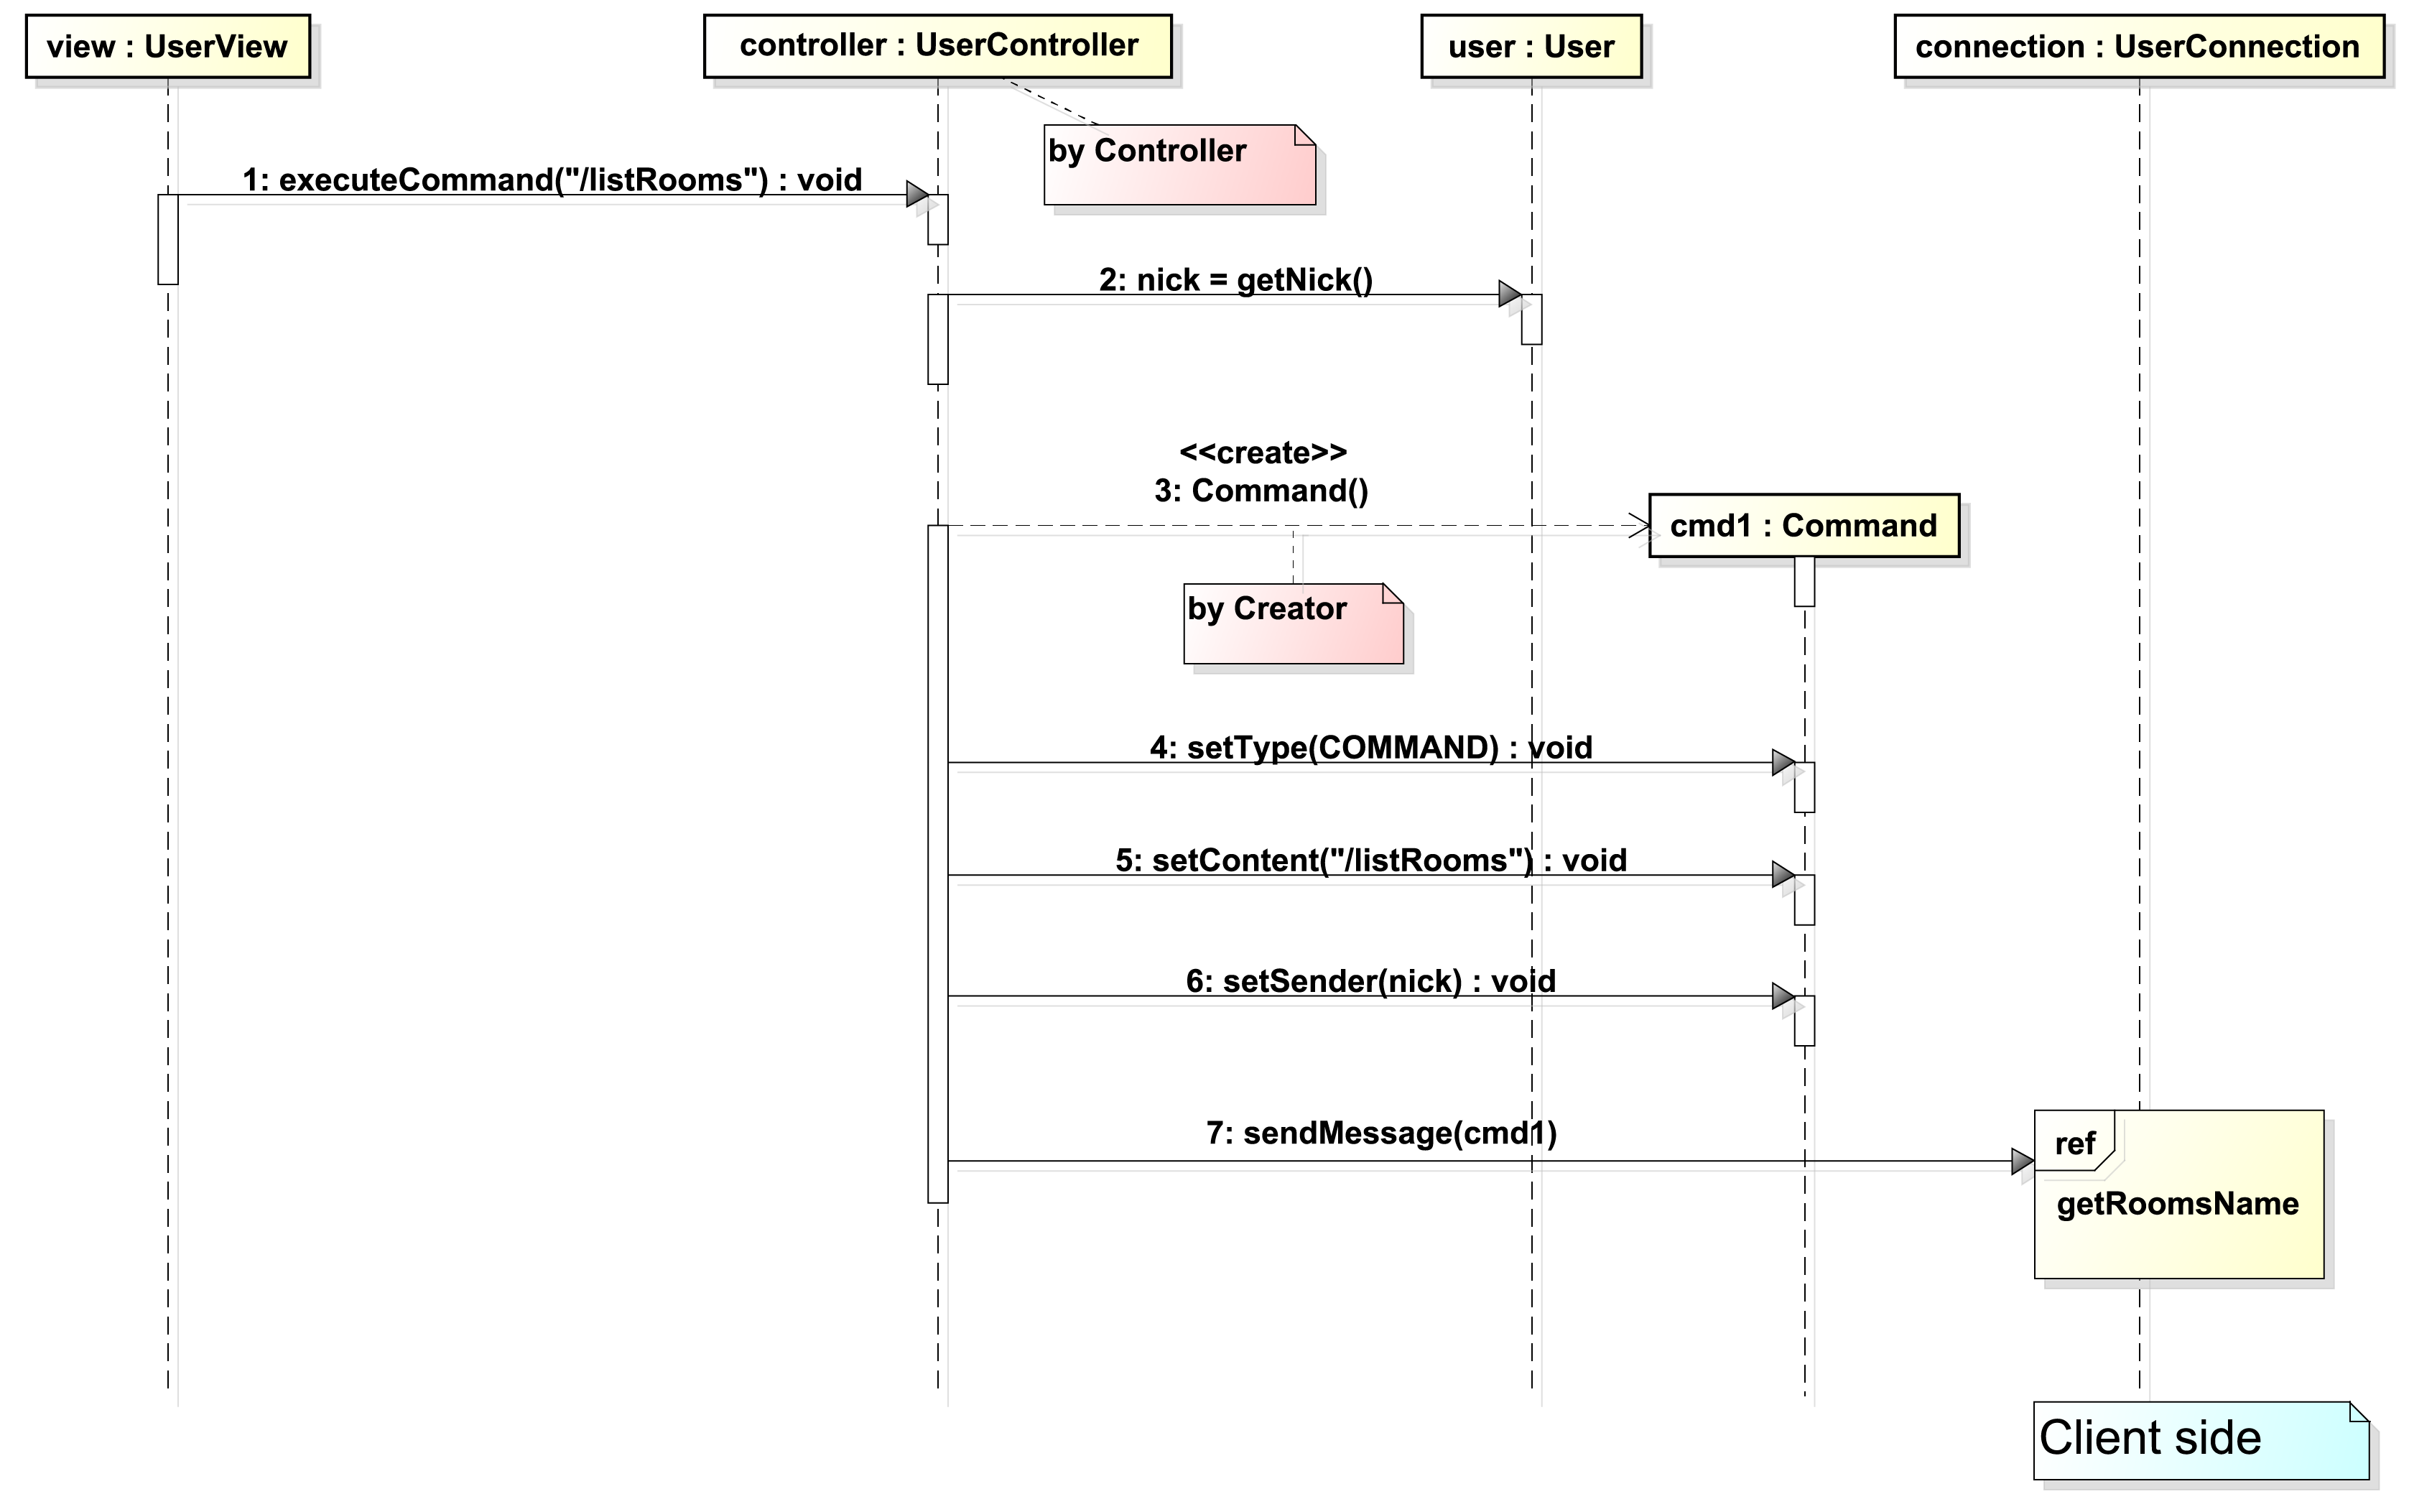
\includegraphics[scale=0.17]{image_astah/Iteration_1_DesignModel/UC2_AccessRoom_SSD_1_sendCommand.png}{\centering}
     \caption{SSD - OP1: sendCommand(cmd1) del modello di dominio (figura \ref{fig_UC2_AR_SSD}) }
     \label{fig_UC2_SSD_AC_1} 
   \end{figure}
\end{frame}

\begin{frame} {Iterazione 1: Progettazione, UC2\_AccessRoom - OP2}
   \begin{figure}
     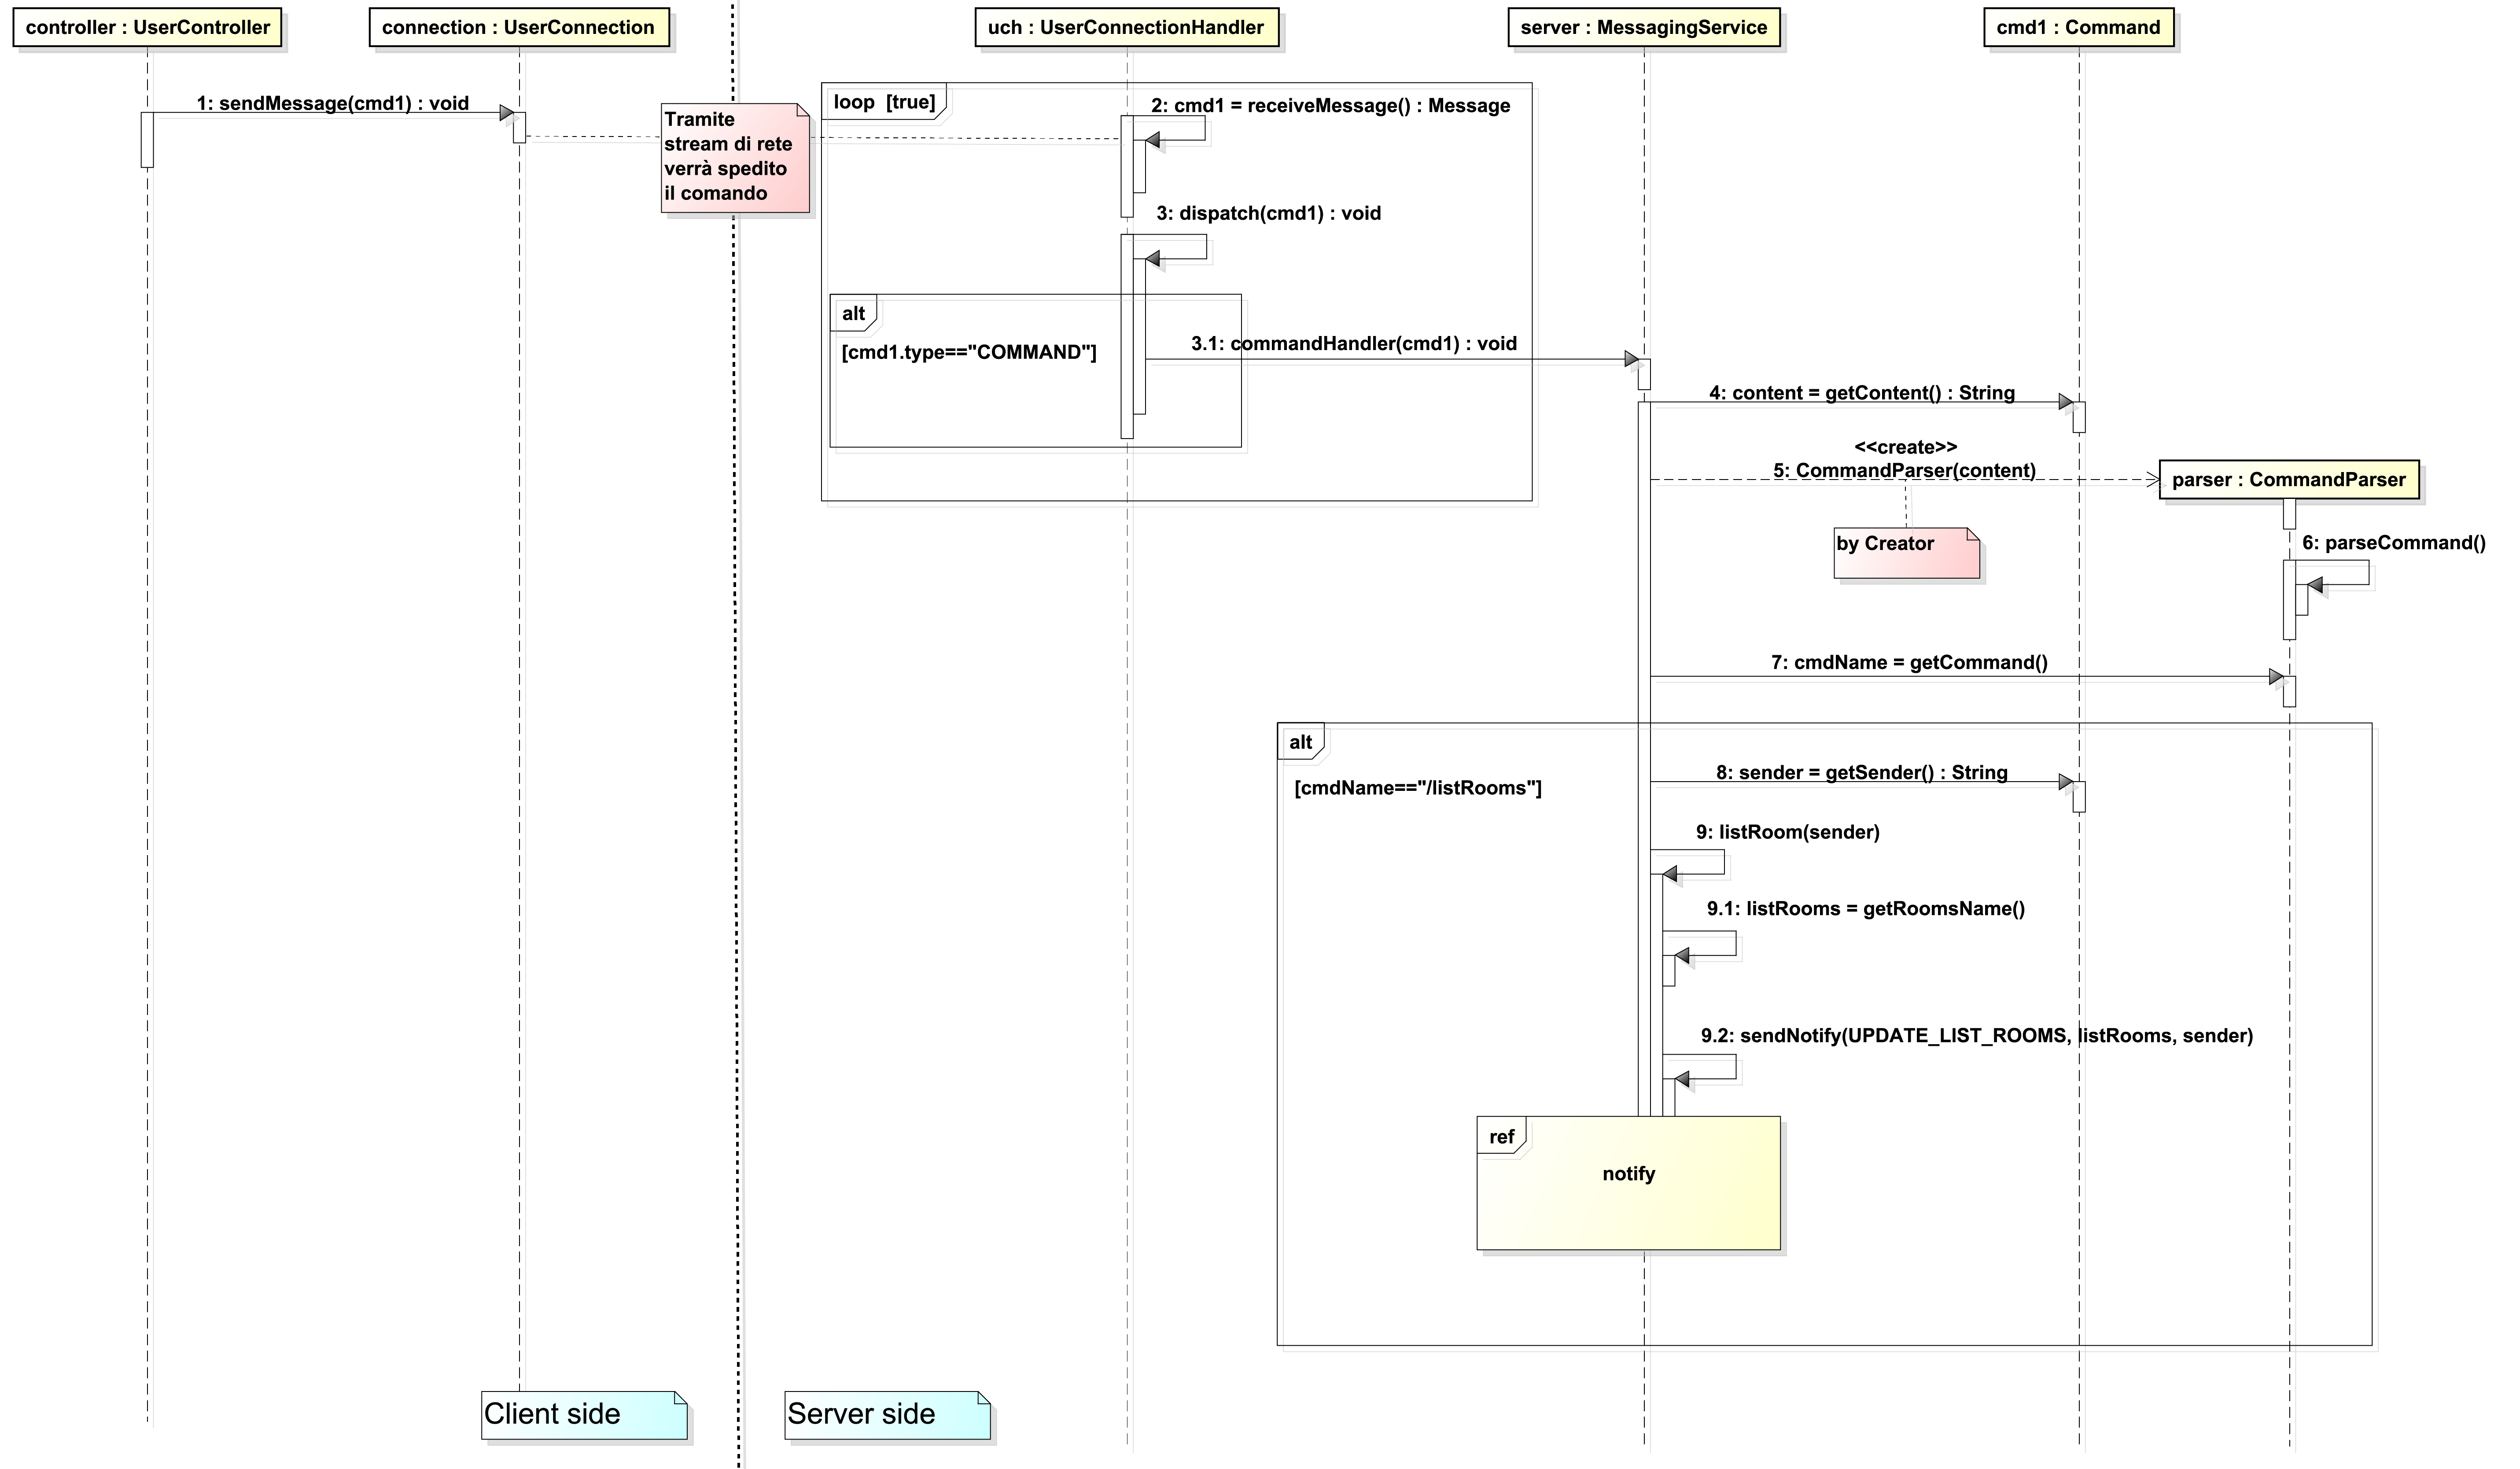
\includegraphics[scale=0.11]{image_astah/Iteration_1_DesignModel/UC2_AccessRoom_SSD_2_getRoomsName.png}{\centering}
     \caption{SSD - OP2: getRoomsName() del modello di dominio (figura \ref{fig_UC2_AR_SSD}) }
     \label{fig_UC2_SSD_AC_2} 
   \end{figure}
\end{frame}

\begin{frame} {Iterazione 1: Progettazione, UC2\_AccessRoom - OP3}
   \begin{figure}
     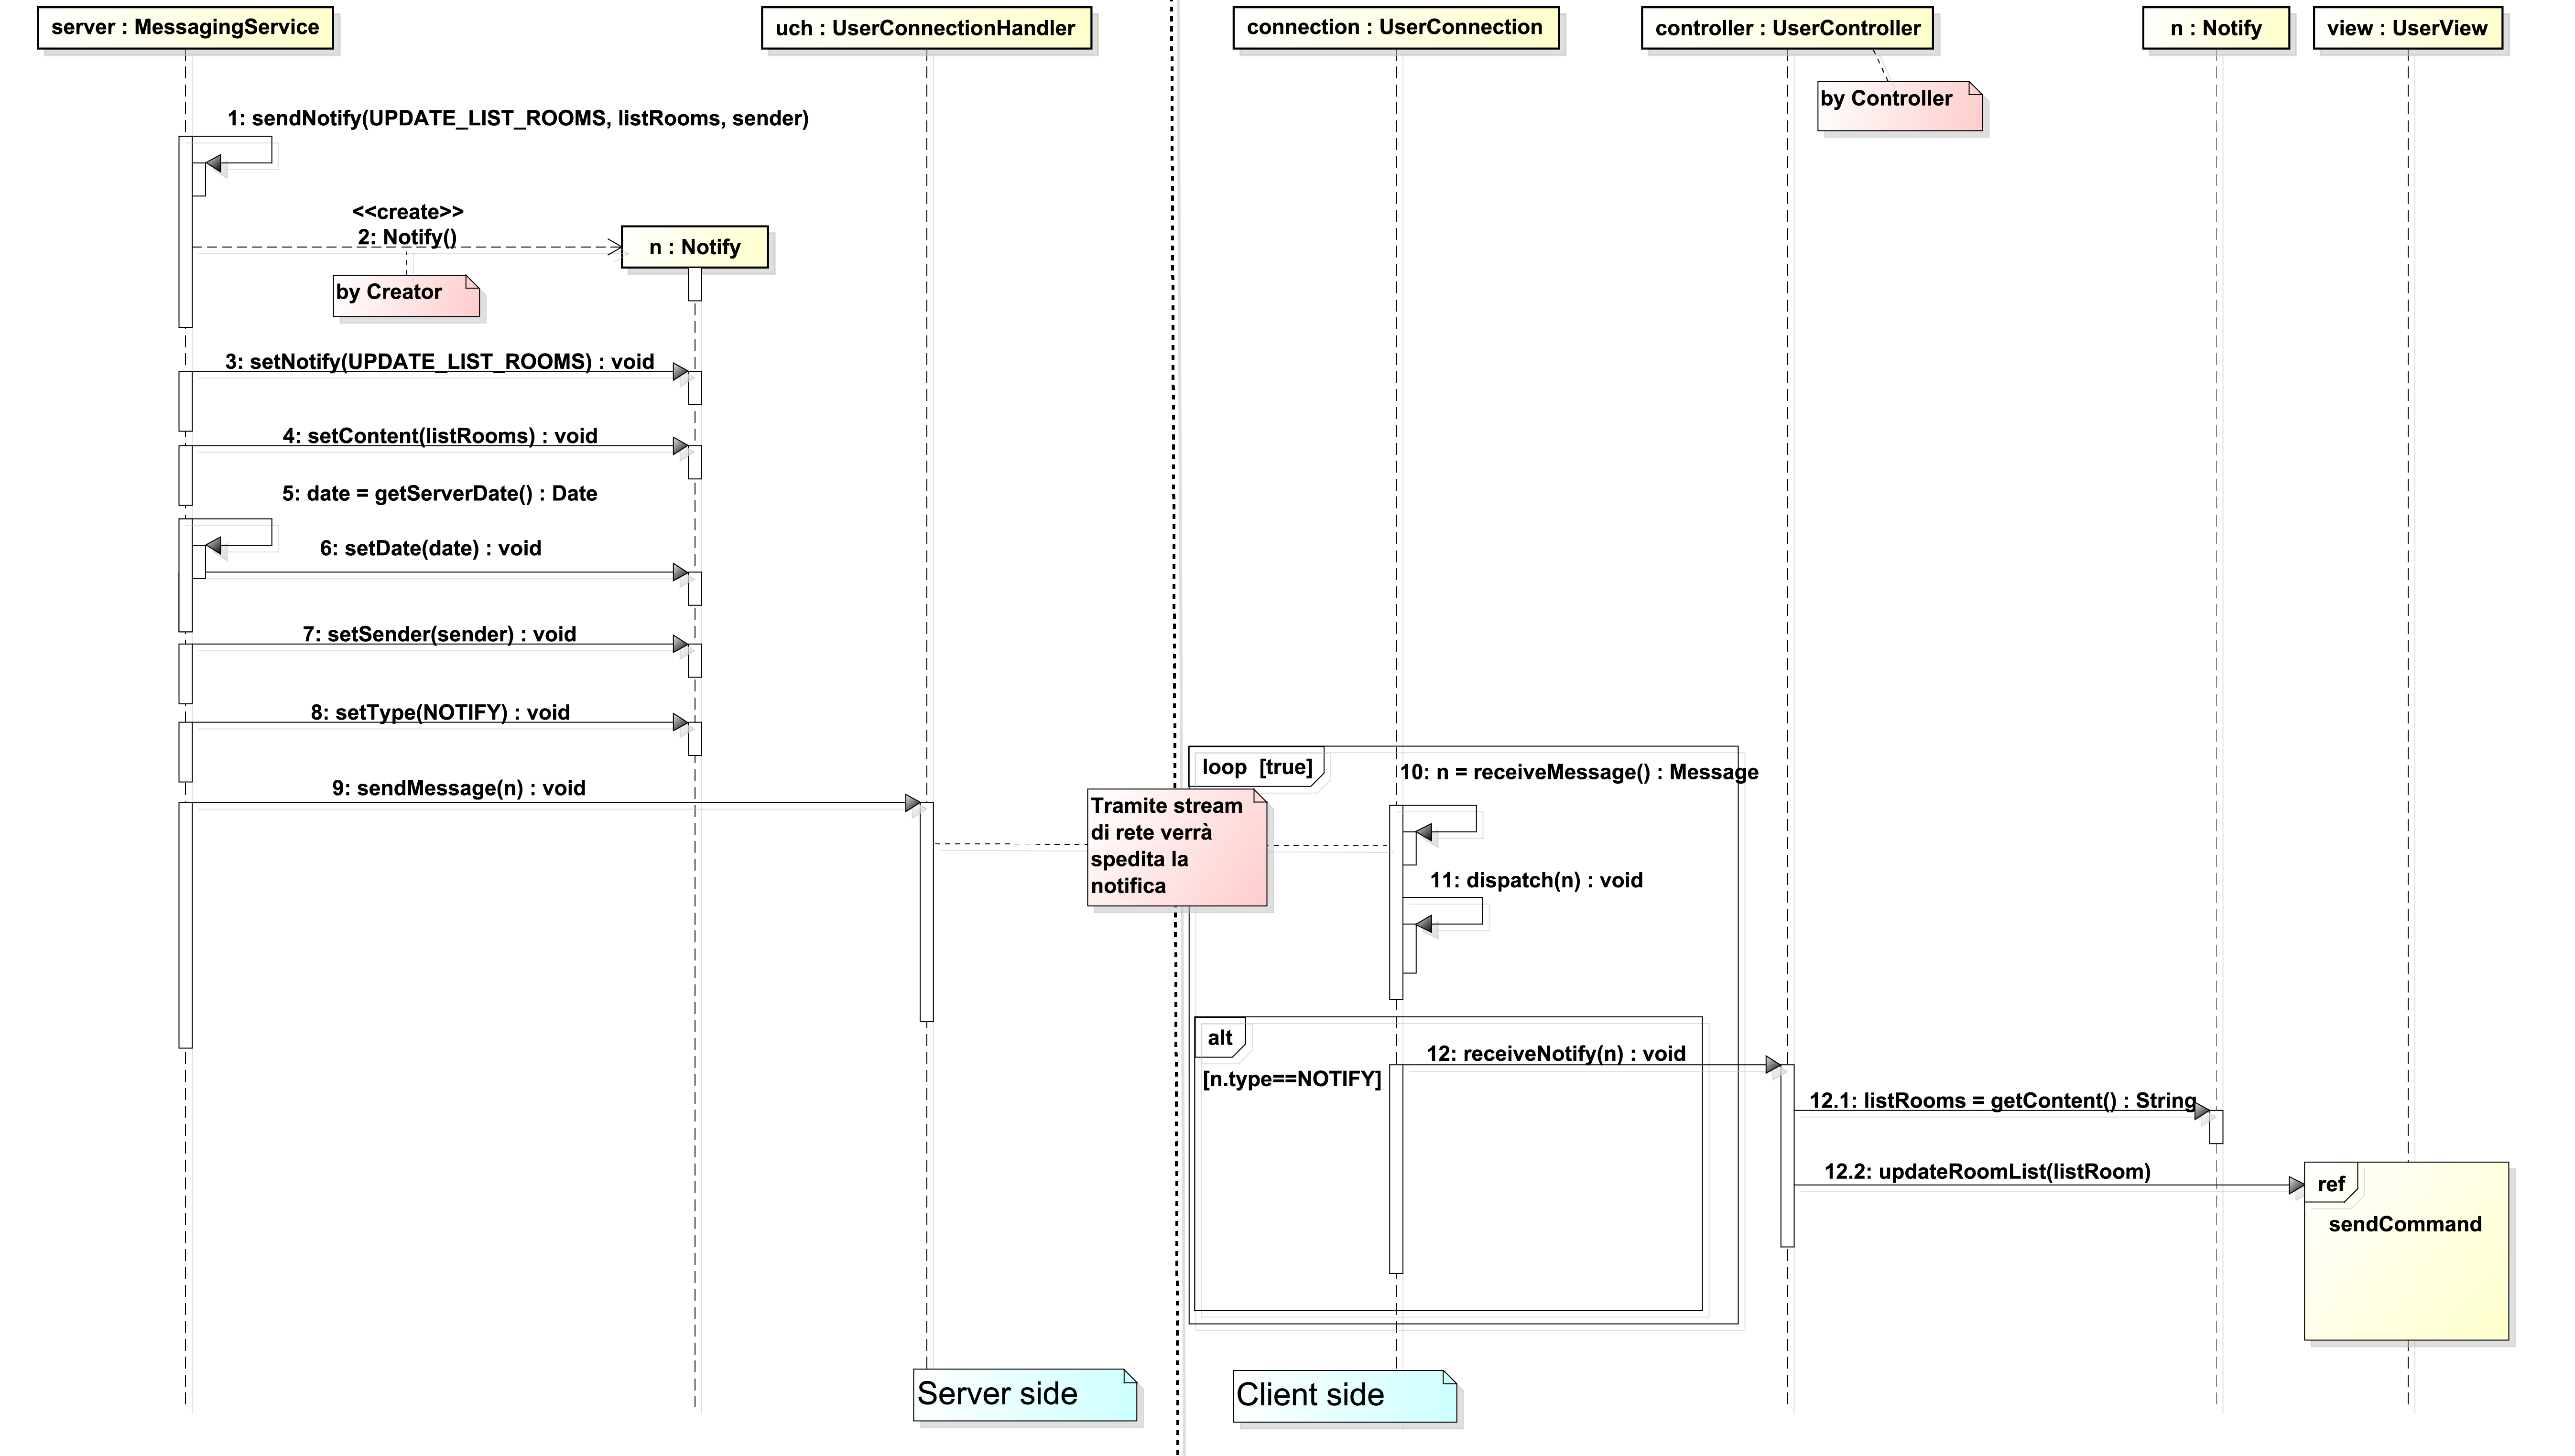
\includegraphics[scale=0.12]{image_astah/Iteration_1_DesignModel/UC2_AccessRoom_SSD_3_notify.png}{\centering}
     \caption{SSD - OP3: notify(list) del modello di dominio (figura \ref{fig_UC2_AR_SSD})}
     \label{fig_UC2_SSD_AC_3} 
   \end{figure}
\end{frame}

\begin{frame} {Iterazione 1: Progettazione, UC2\_AccessRoom - OP4}
   \begin{figure}
     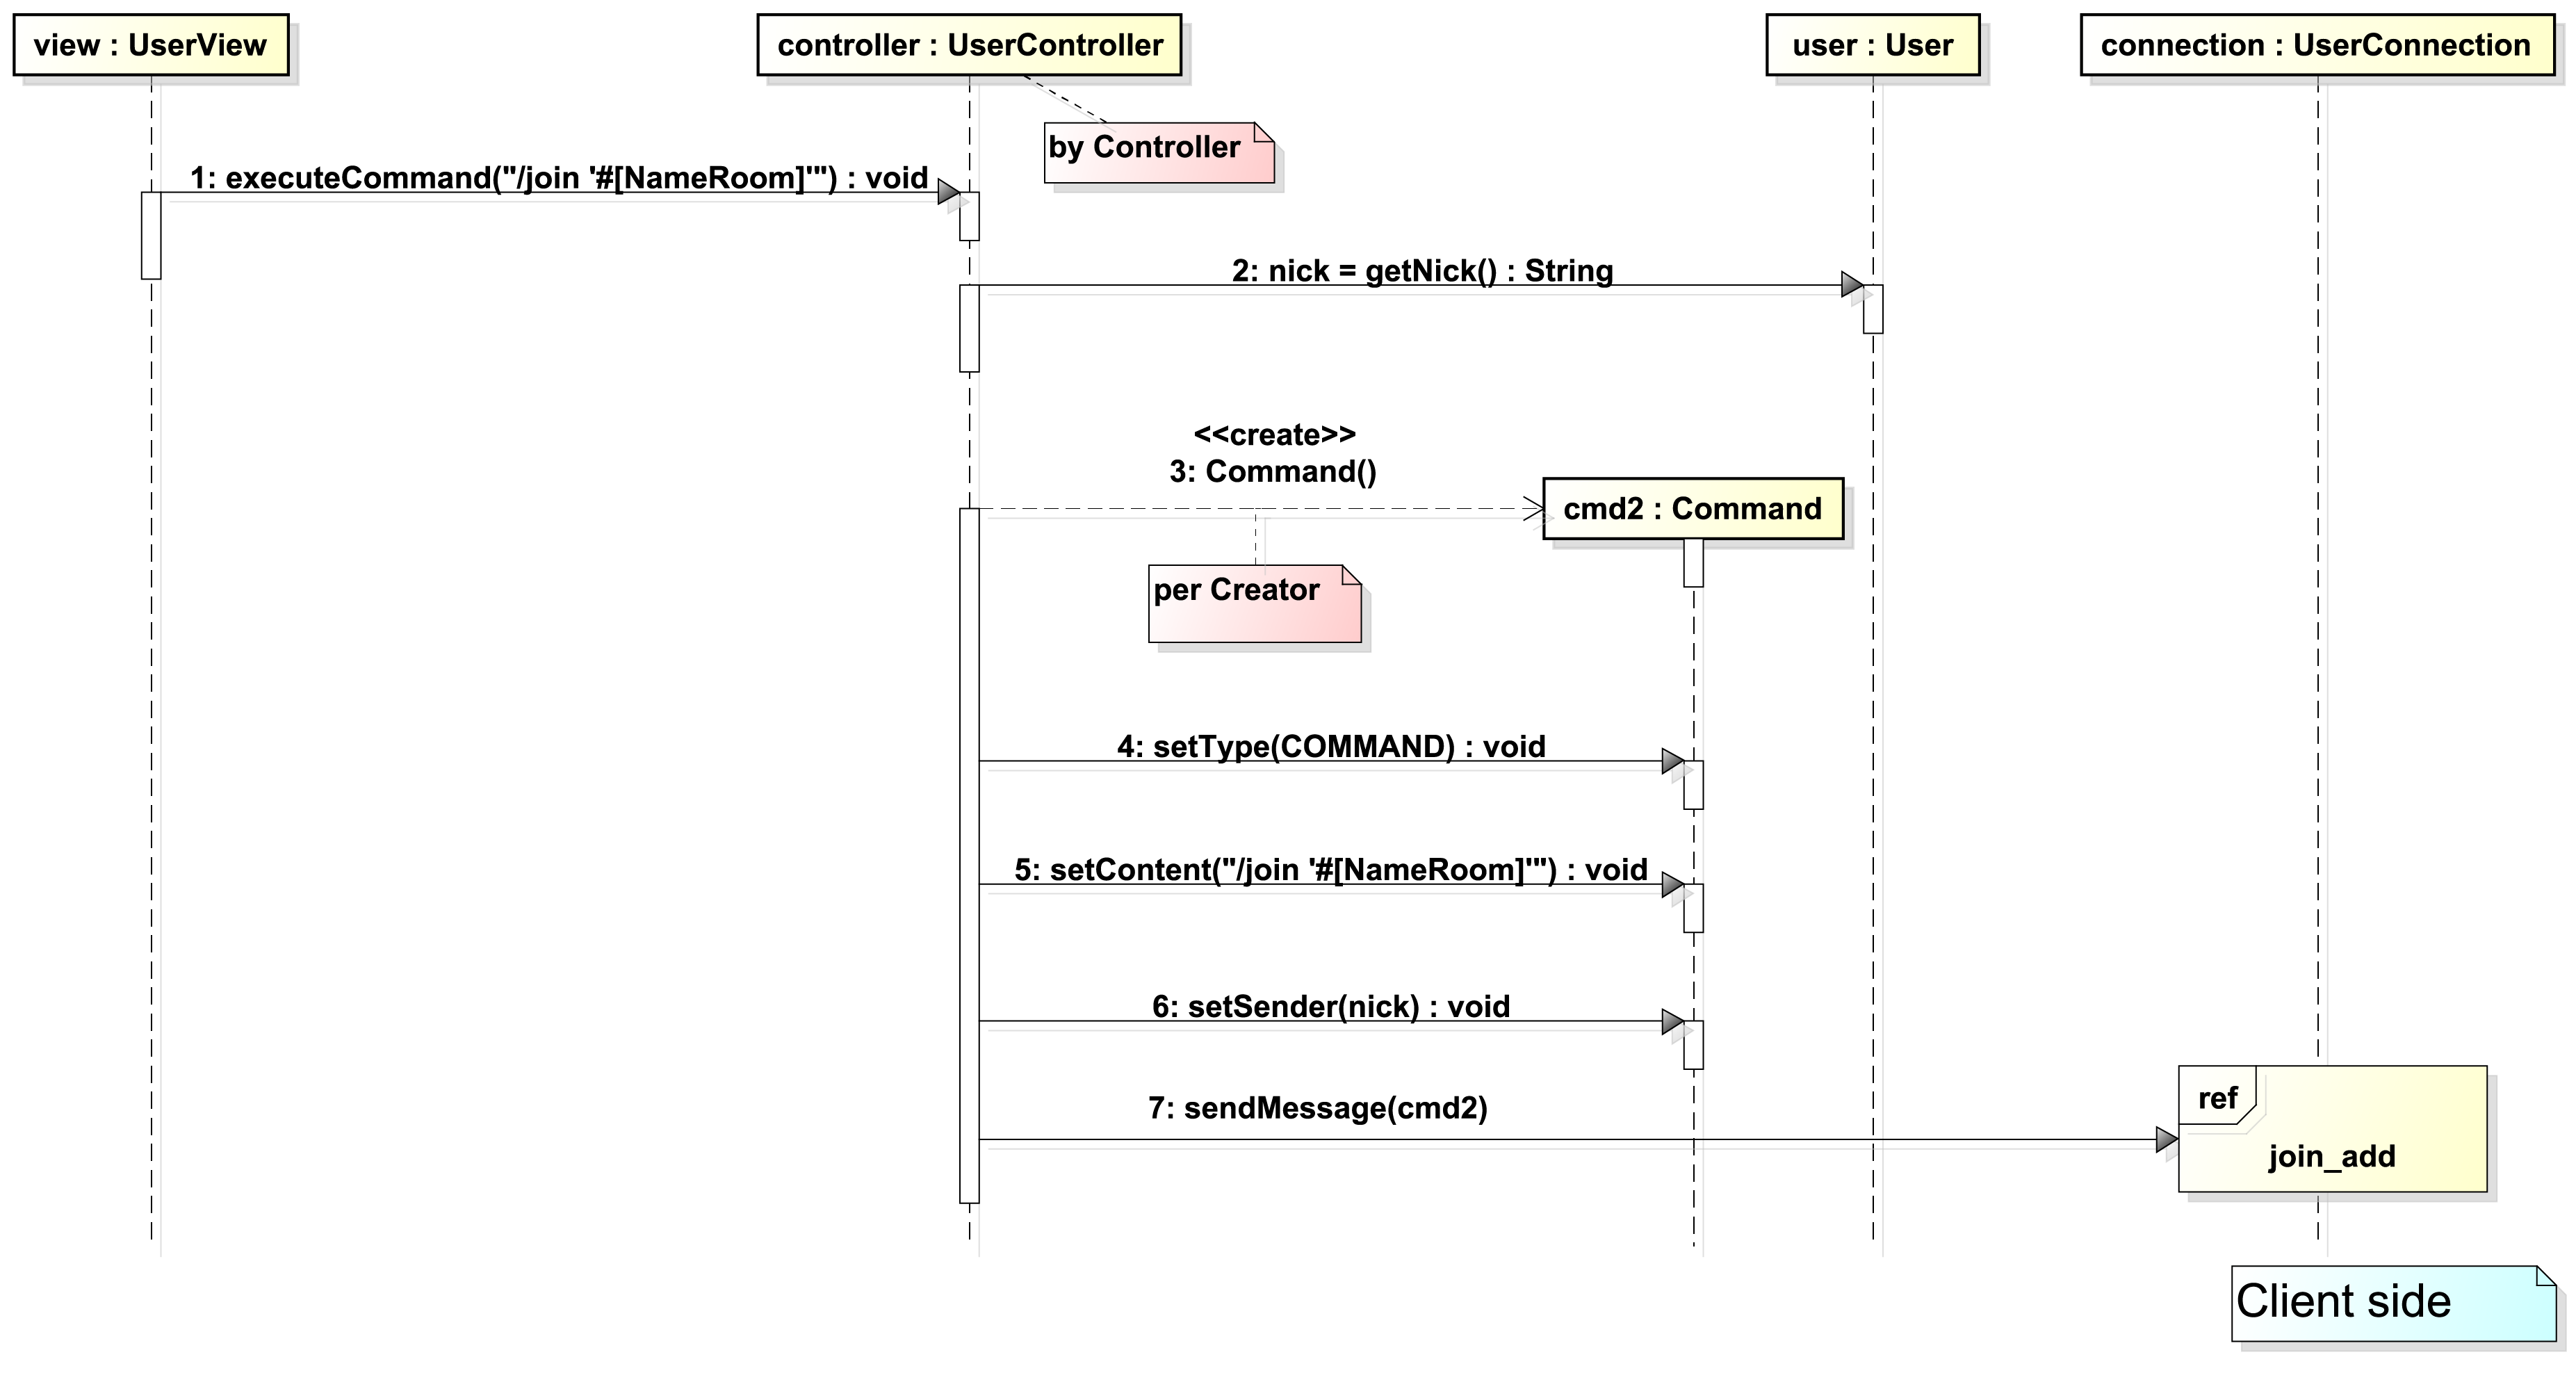
\includegraphics[scale=0.18]{image_astah/Iteration_1_DesignModel/UC2_AccessRoom_SSD_4_sendCommand.png}{\centering}
     \caption{SSD - OP4: sendCommand(cmd2) del modello di dominio (figura \ref{fig_UC2_AR_SSD}) }
     \label{fig_UC2_SSD_AC_4} 
   \end{figure}
\end{frame}

\begin{frame} {Iterazione 1: Progettazione, UC2\_AccessRoom - OP5}
   \begin{figure}
     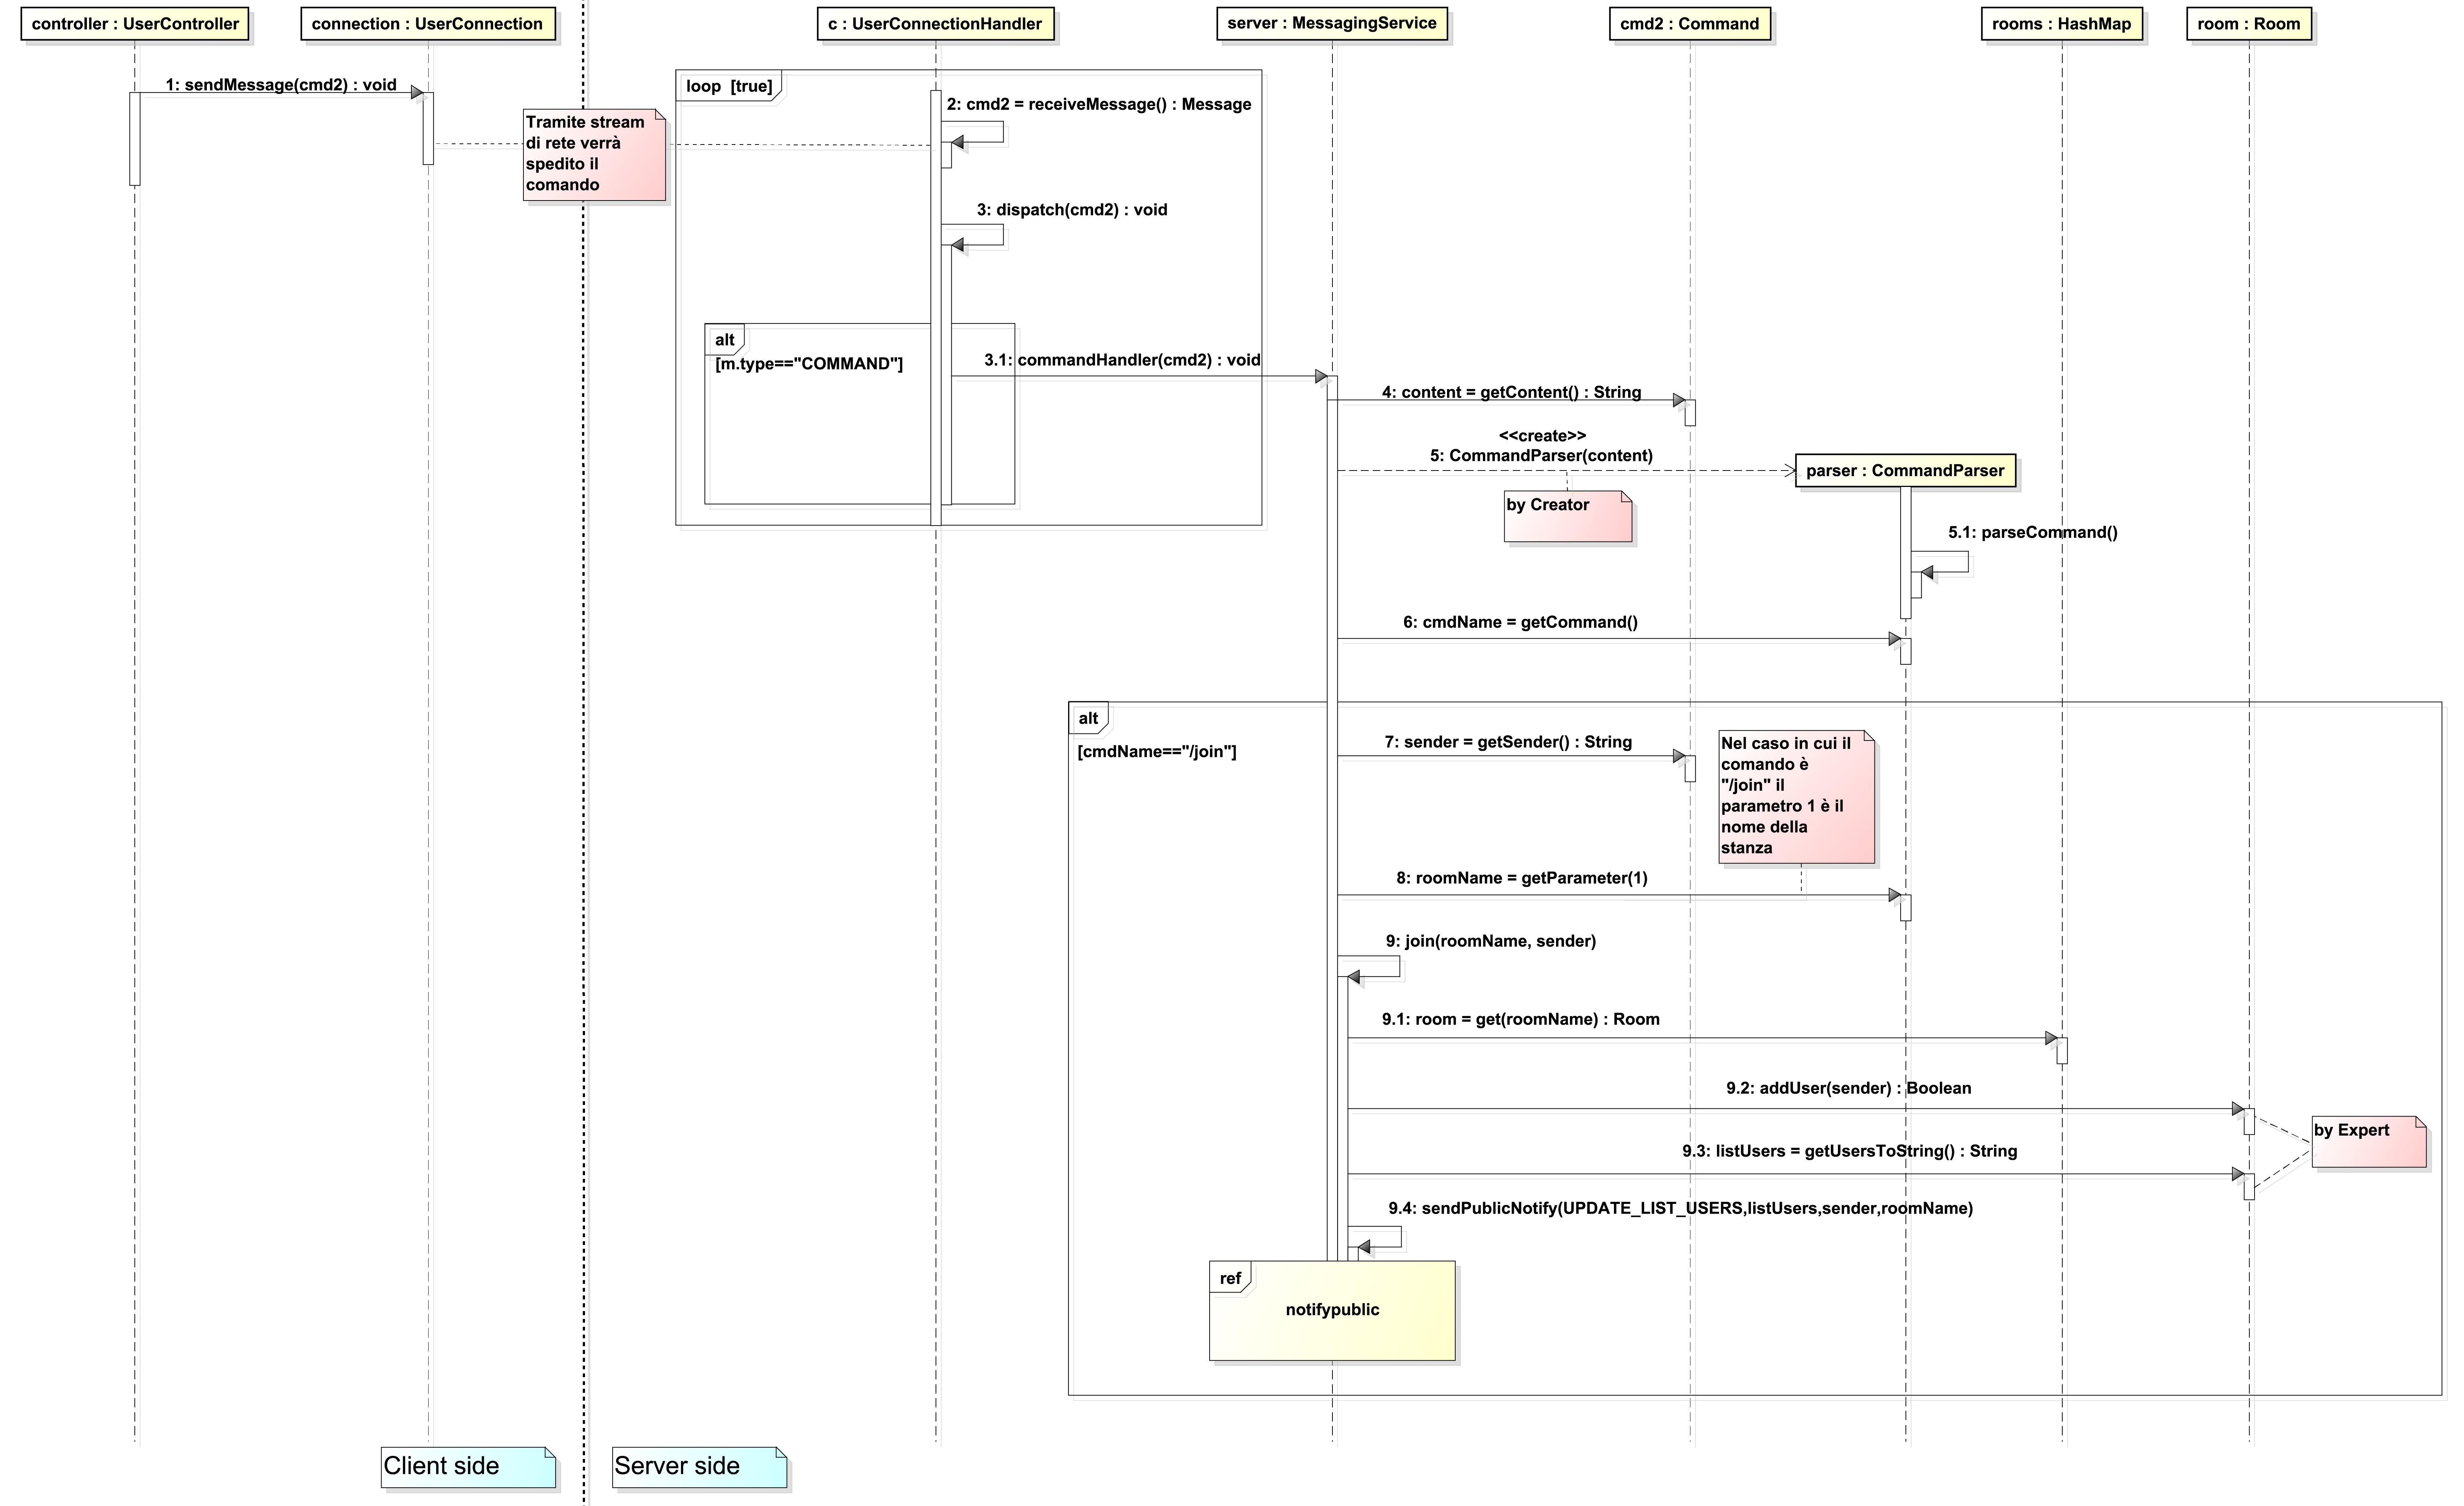
\includegraphics[scale=0.09]{image_astah/Iteration_1_DesignModel/UC2_AccessRoom_SSD_5_join_add.png}{\centering}
     \caption{SSD - OP5: joinRoom(sender,room), addUserToRoom() del modello di dominio (figura \ref{fig_UC2_AR_SSD}) }
     \label{fig_UC2_SSD_AC_5} 
   \end{figure}
\end{frame}

\begin{frame} {Iterazione 1: Progettazione, UC2\_AccessRoom - OP6}
   \begin{figure}
     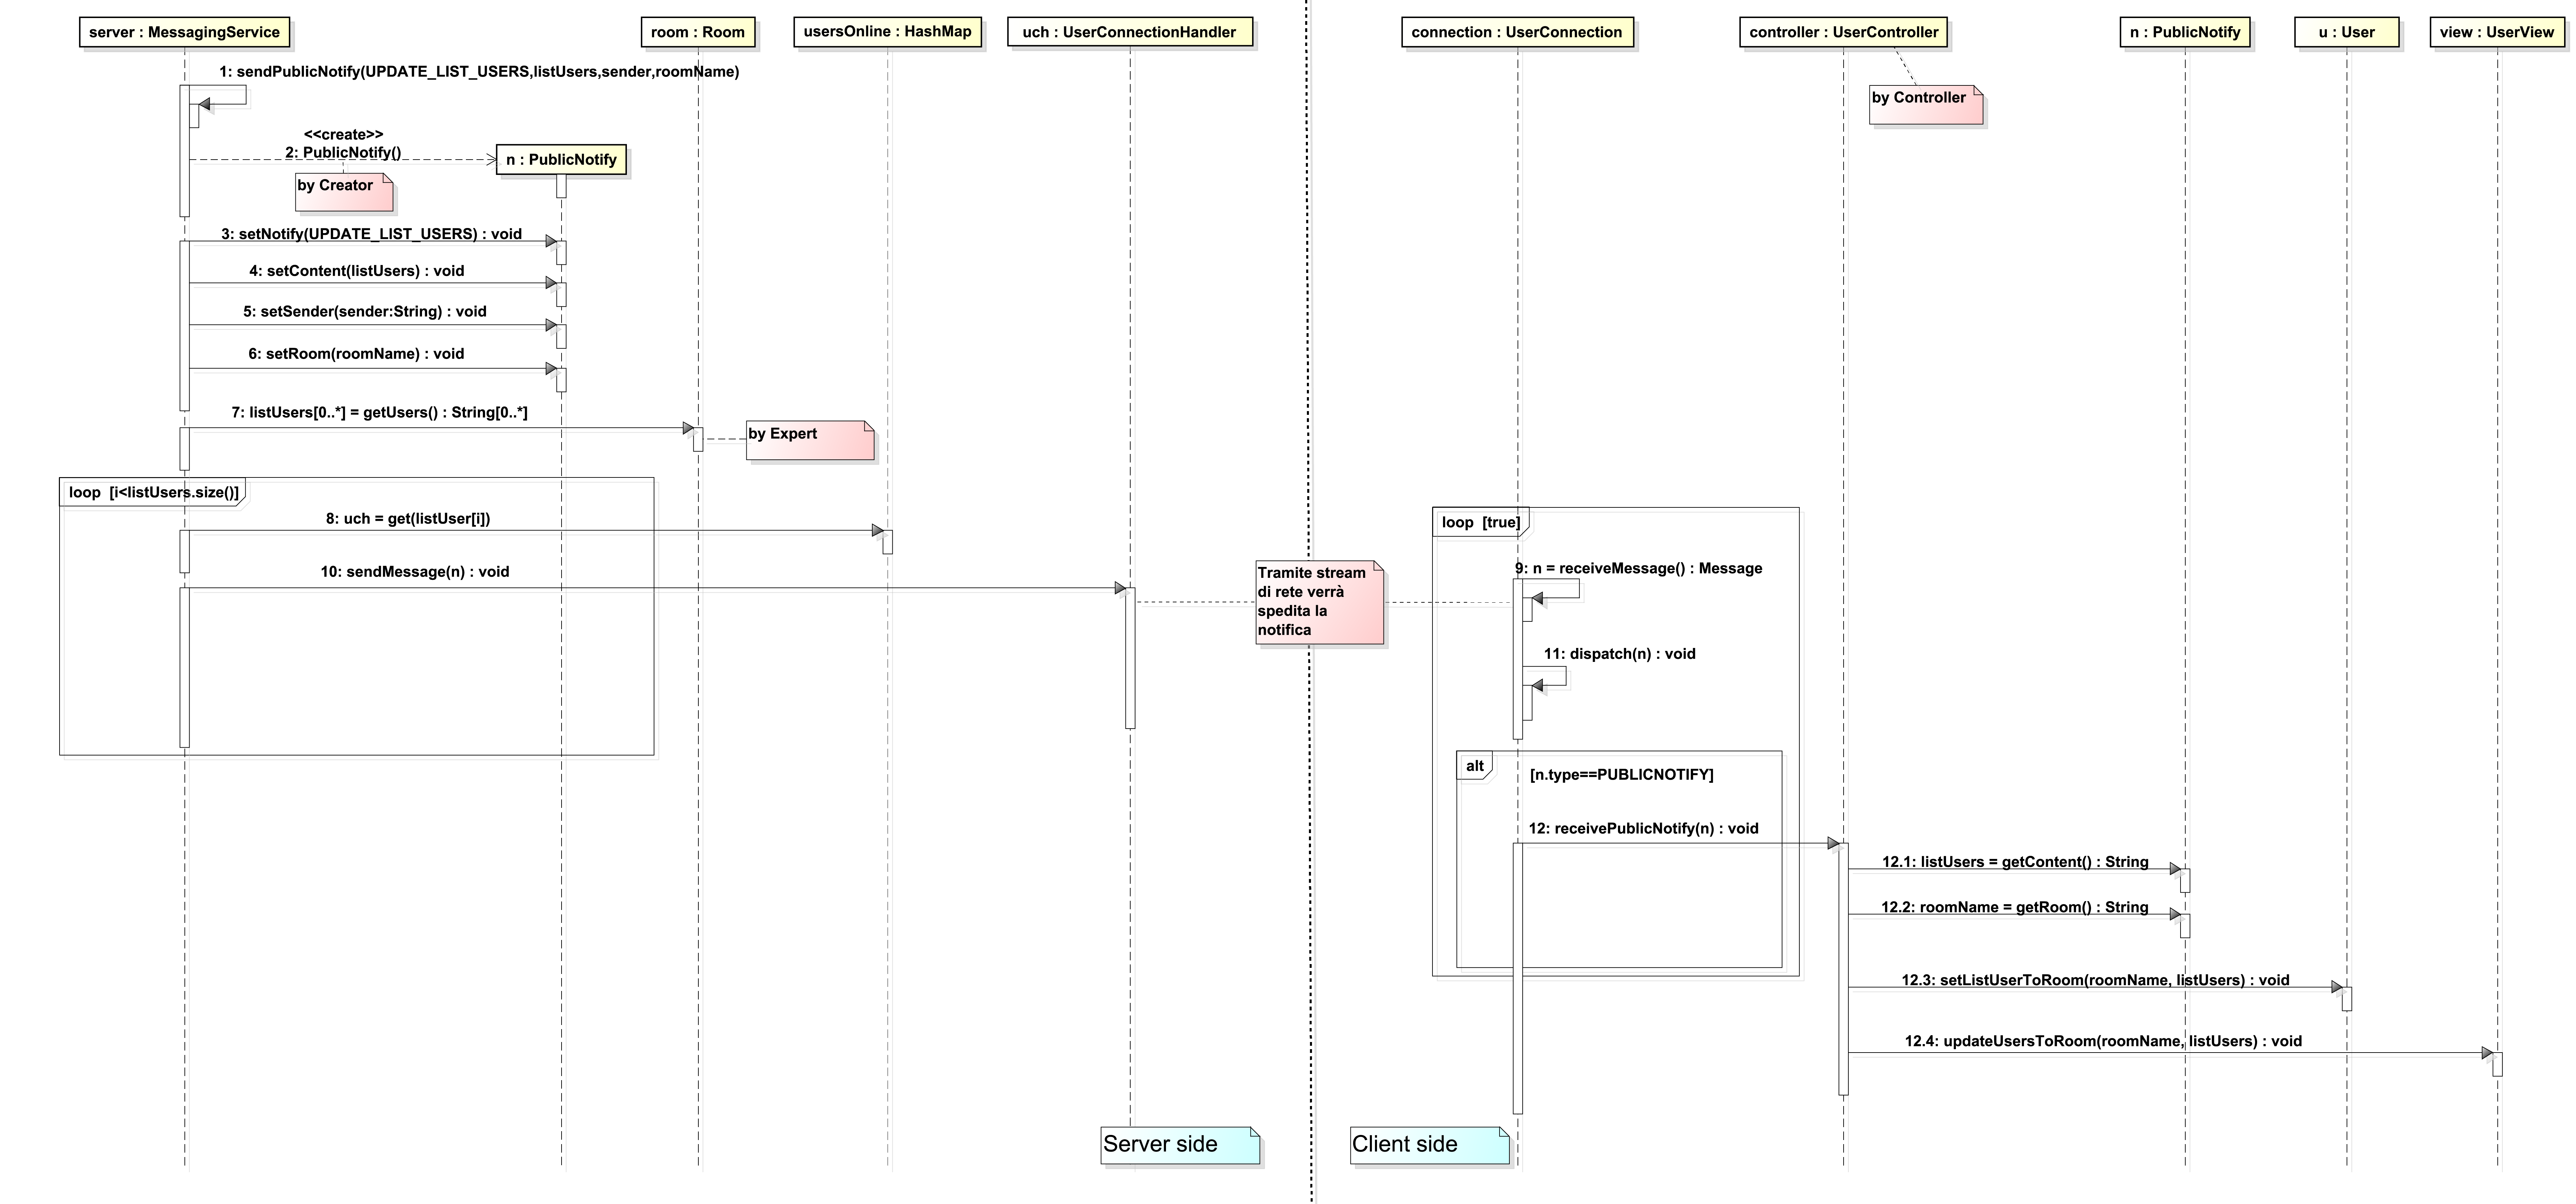
\includegraphics[scale=0.09]{image_astah/Iteration_1_DesignModel/UC2_AccessRoom_SSD_6_notifypublic.png}{\centering}
     \caption{SSD - OP6: notifypublic(updateList) del modello di dominio (figura \ref{fig_UC2_AR_SSD}) }
     \label{fig_UC2_SSD_AC_6} 
   \end{figure}
\end{frame}

%ITERAZIONE 1 REFACTORING PROGETTAZIONE 
\section{Refactoring Iterazione 1}
\begin{frame} {Descrizione: Refactoring Iterazione 1}
 \emph{INSERIRE DESCRIZIONE}
\end{frame}

\subsection{Refactoring Iterazione 1: Class Diagram UC1 e UC2}
\begin{frame} {Refactoring Iterazione 1: Class Diagram Common UC1 e UC2}
   \begin{figure}
     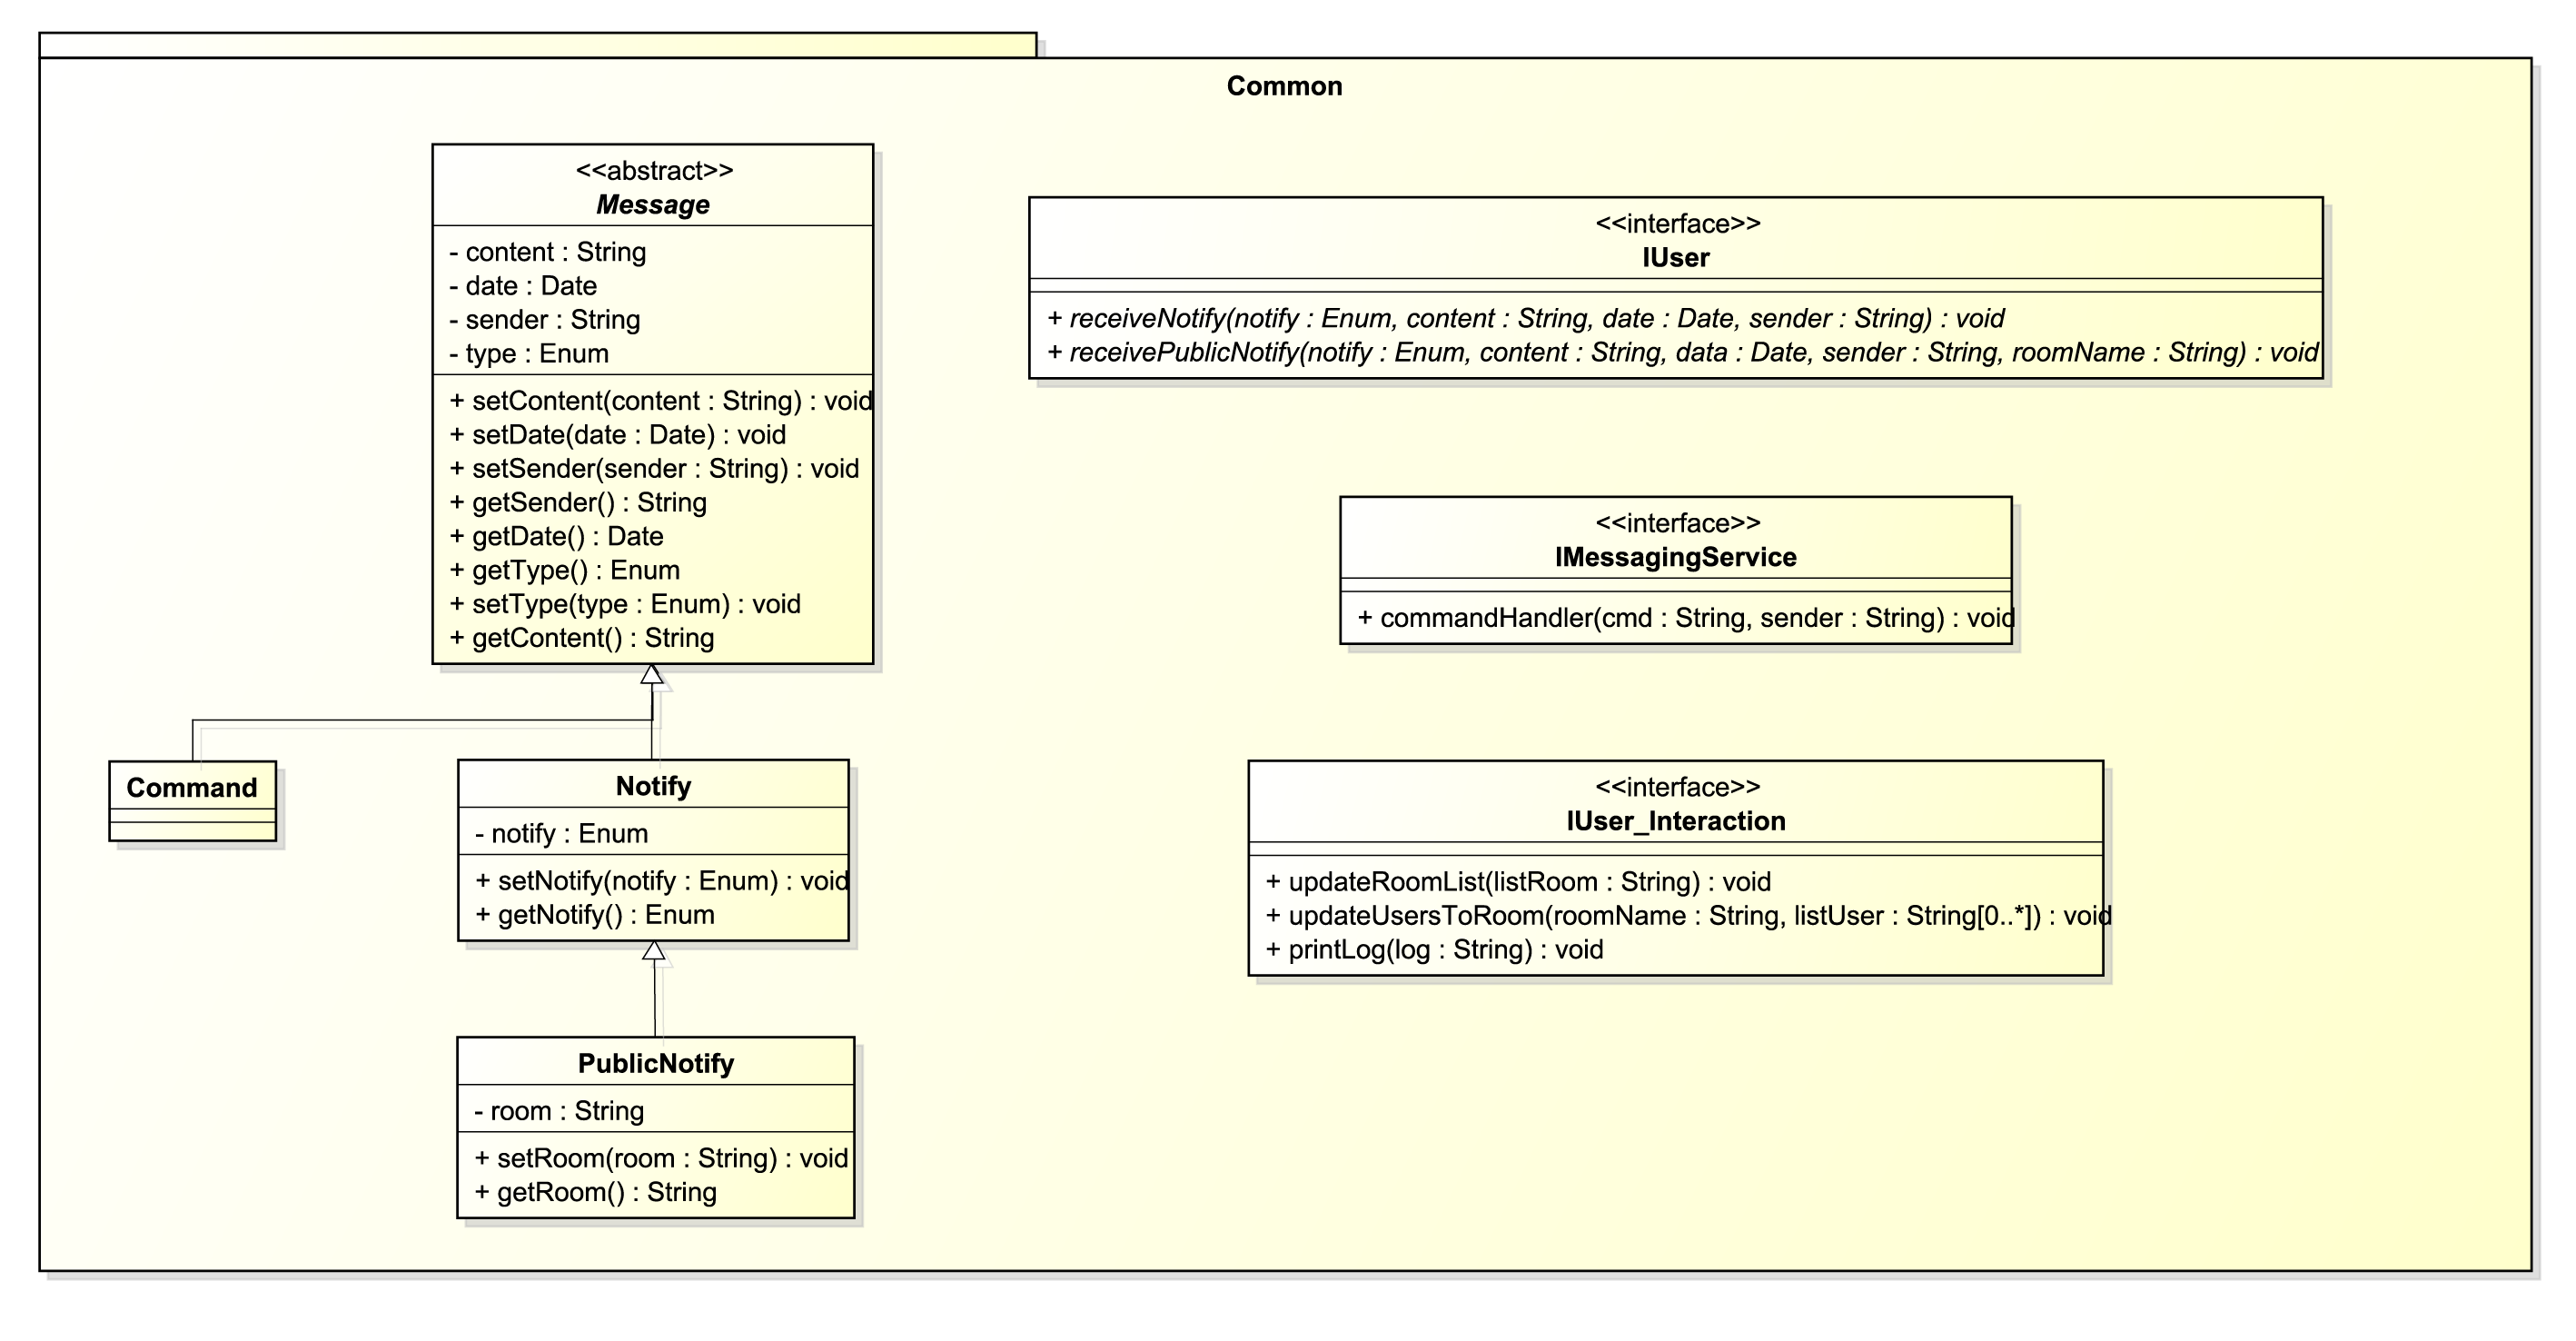
\includegraphics[scale=0.165]{image_astah/Iteration_1_DesignModel_Refactored/ClassDiagramCommon.png}{\centering}
     \caption{DCD - Diagramma delle Classi: Package Common }
     \label{fig_UC1_UC2_DCDR_1} 
   \end{figure}
\end{frame}

\begin{frame} {Refactoring Iterazione 1: Class Diagram Snuc UC1 e UC2}
   \begin{figure}
     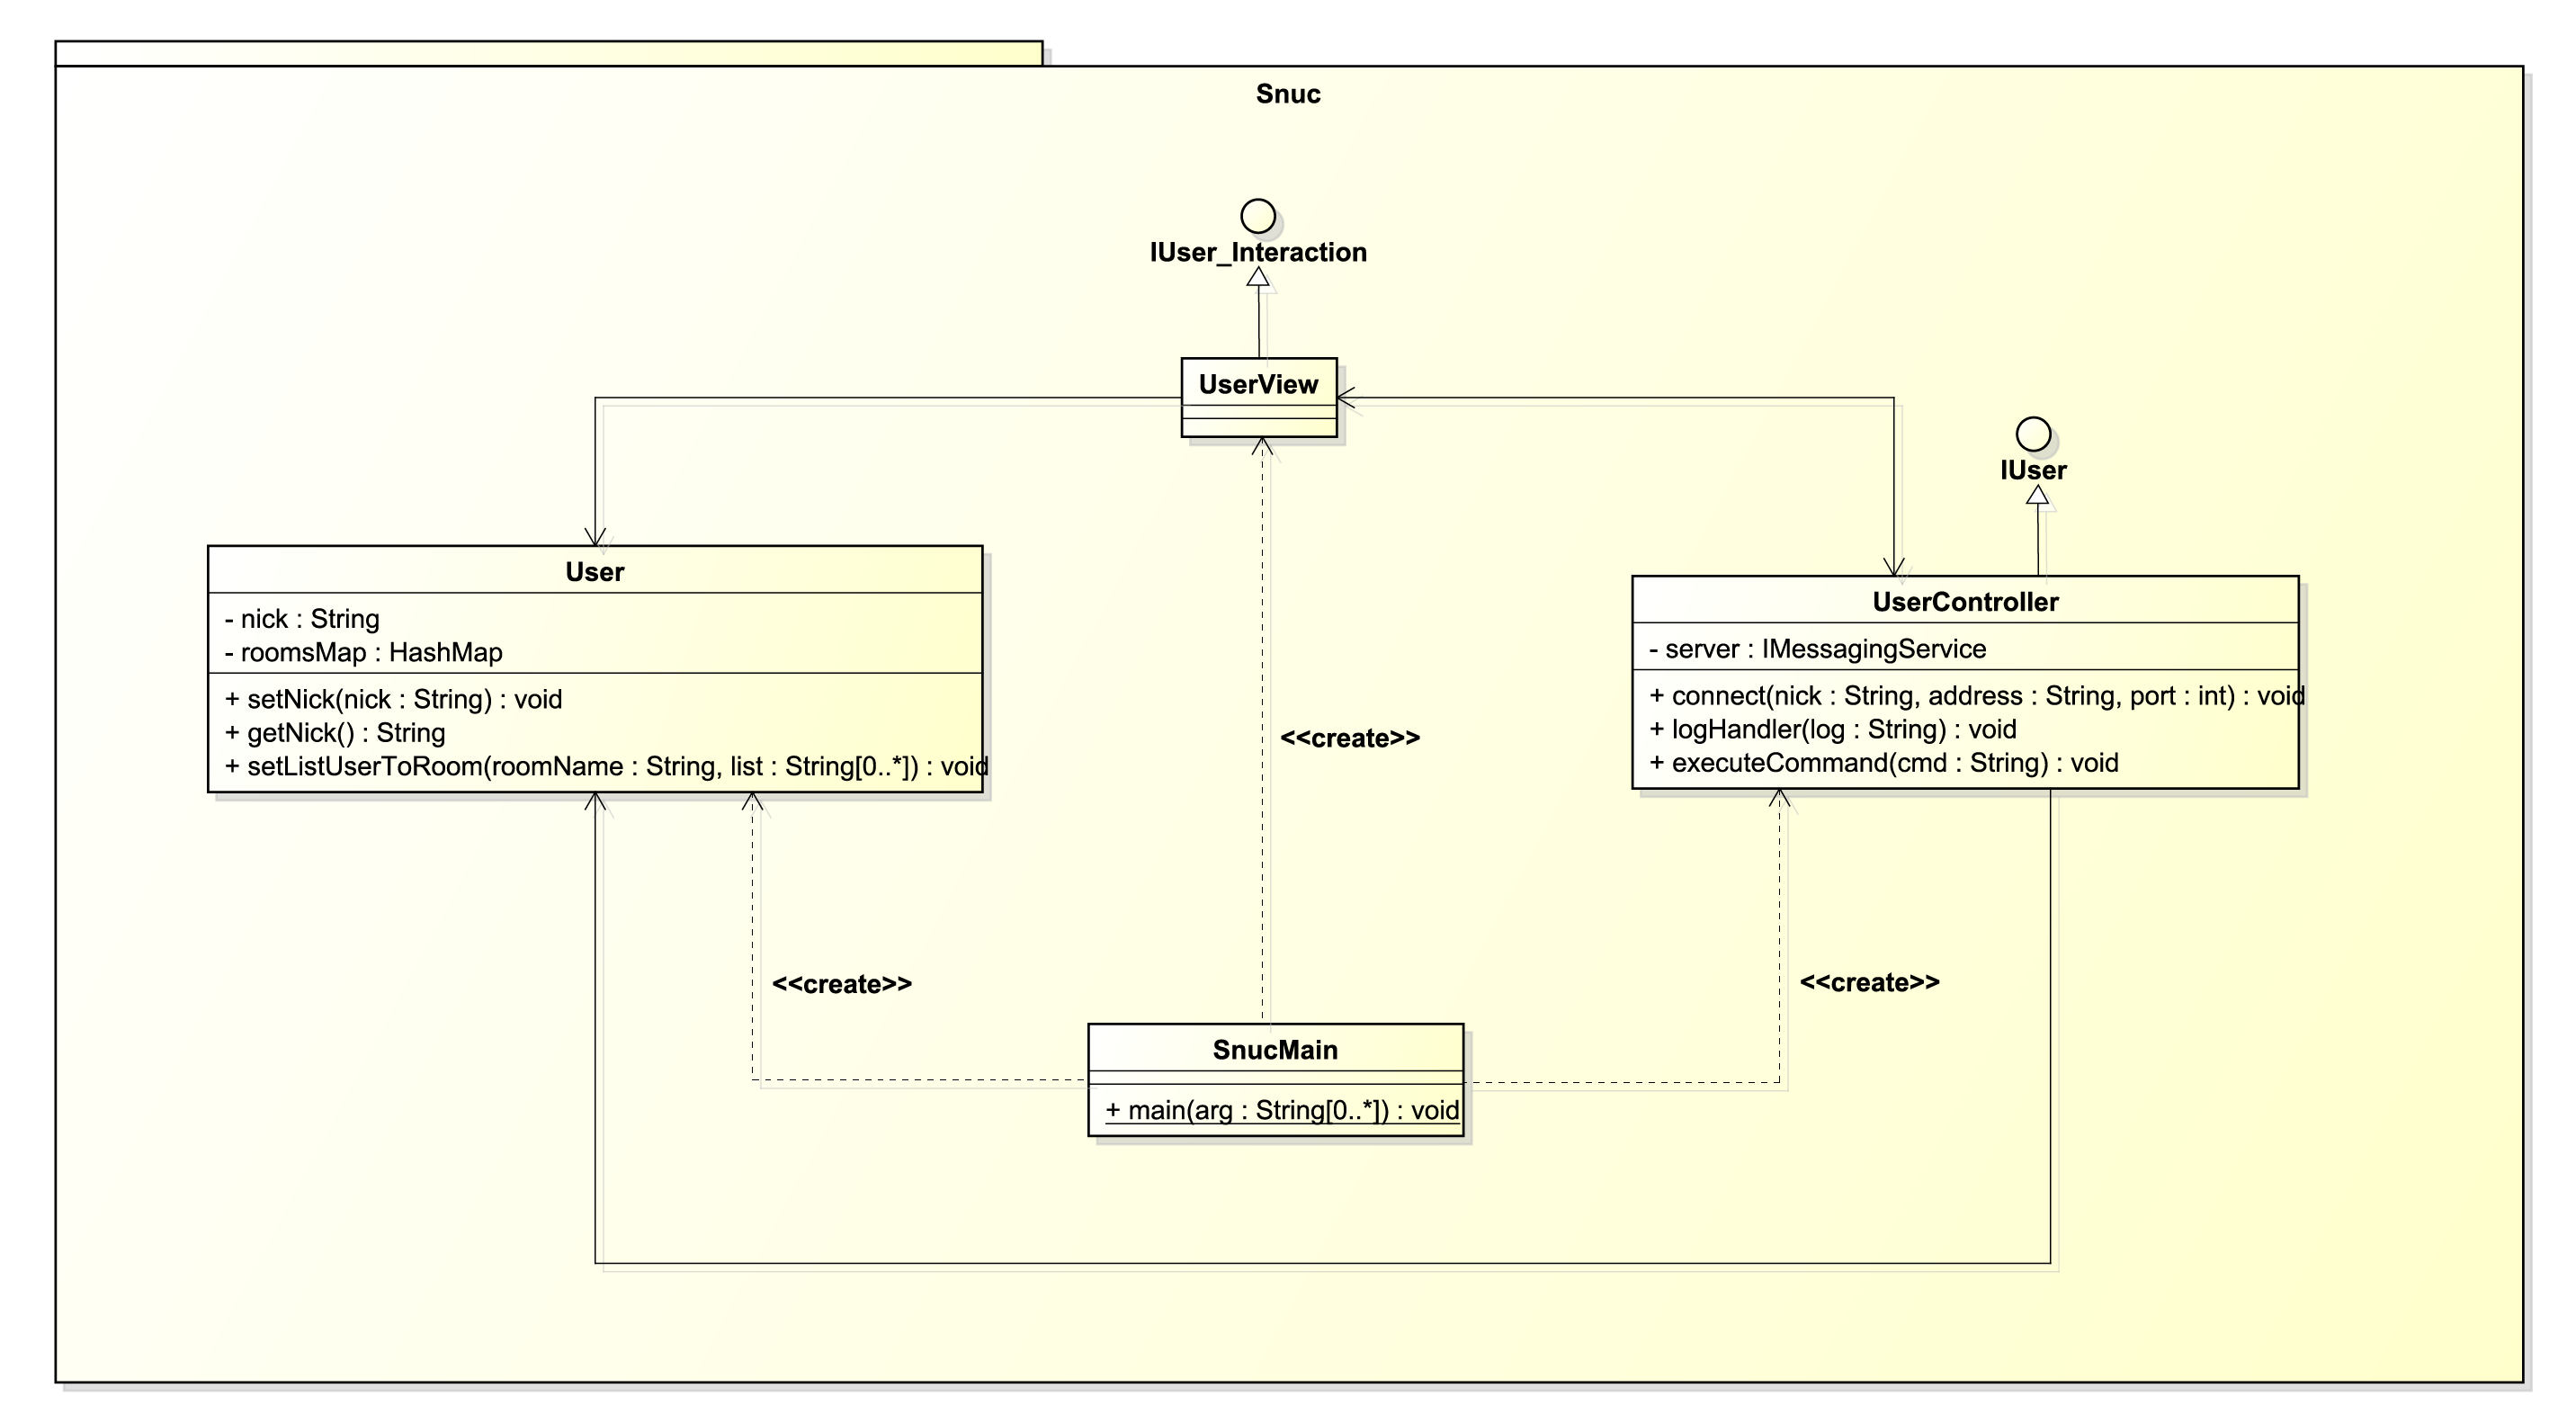
\includegraphics[scale=0.155]{image_astah/Iteration_1_DesignModel_Refactored/ClassDiagramSnuc.png}{\centering}
     \caption{DCD - Diagramma delle Classi: Package Snuc }
     \label{fig_UC1_UC2_DCDR_2} 
   \end{figure}
\end{frame}

\begin{frame} {Refactoring Iterazione 1: Class Diagram Connector UC1 e UC2}
   \begin{figure}
     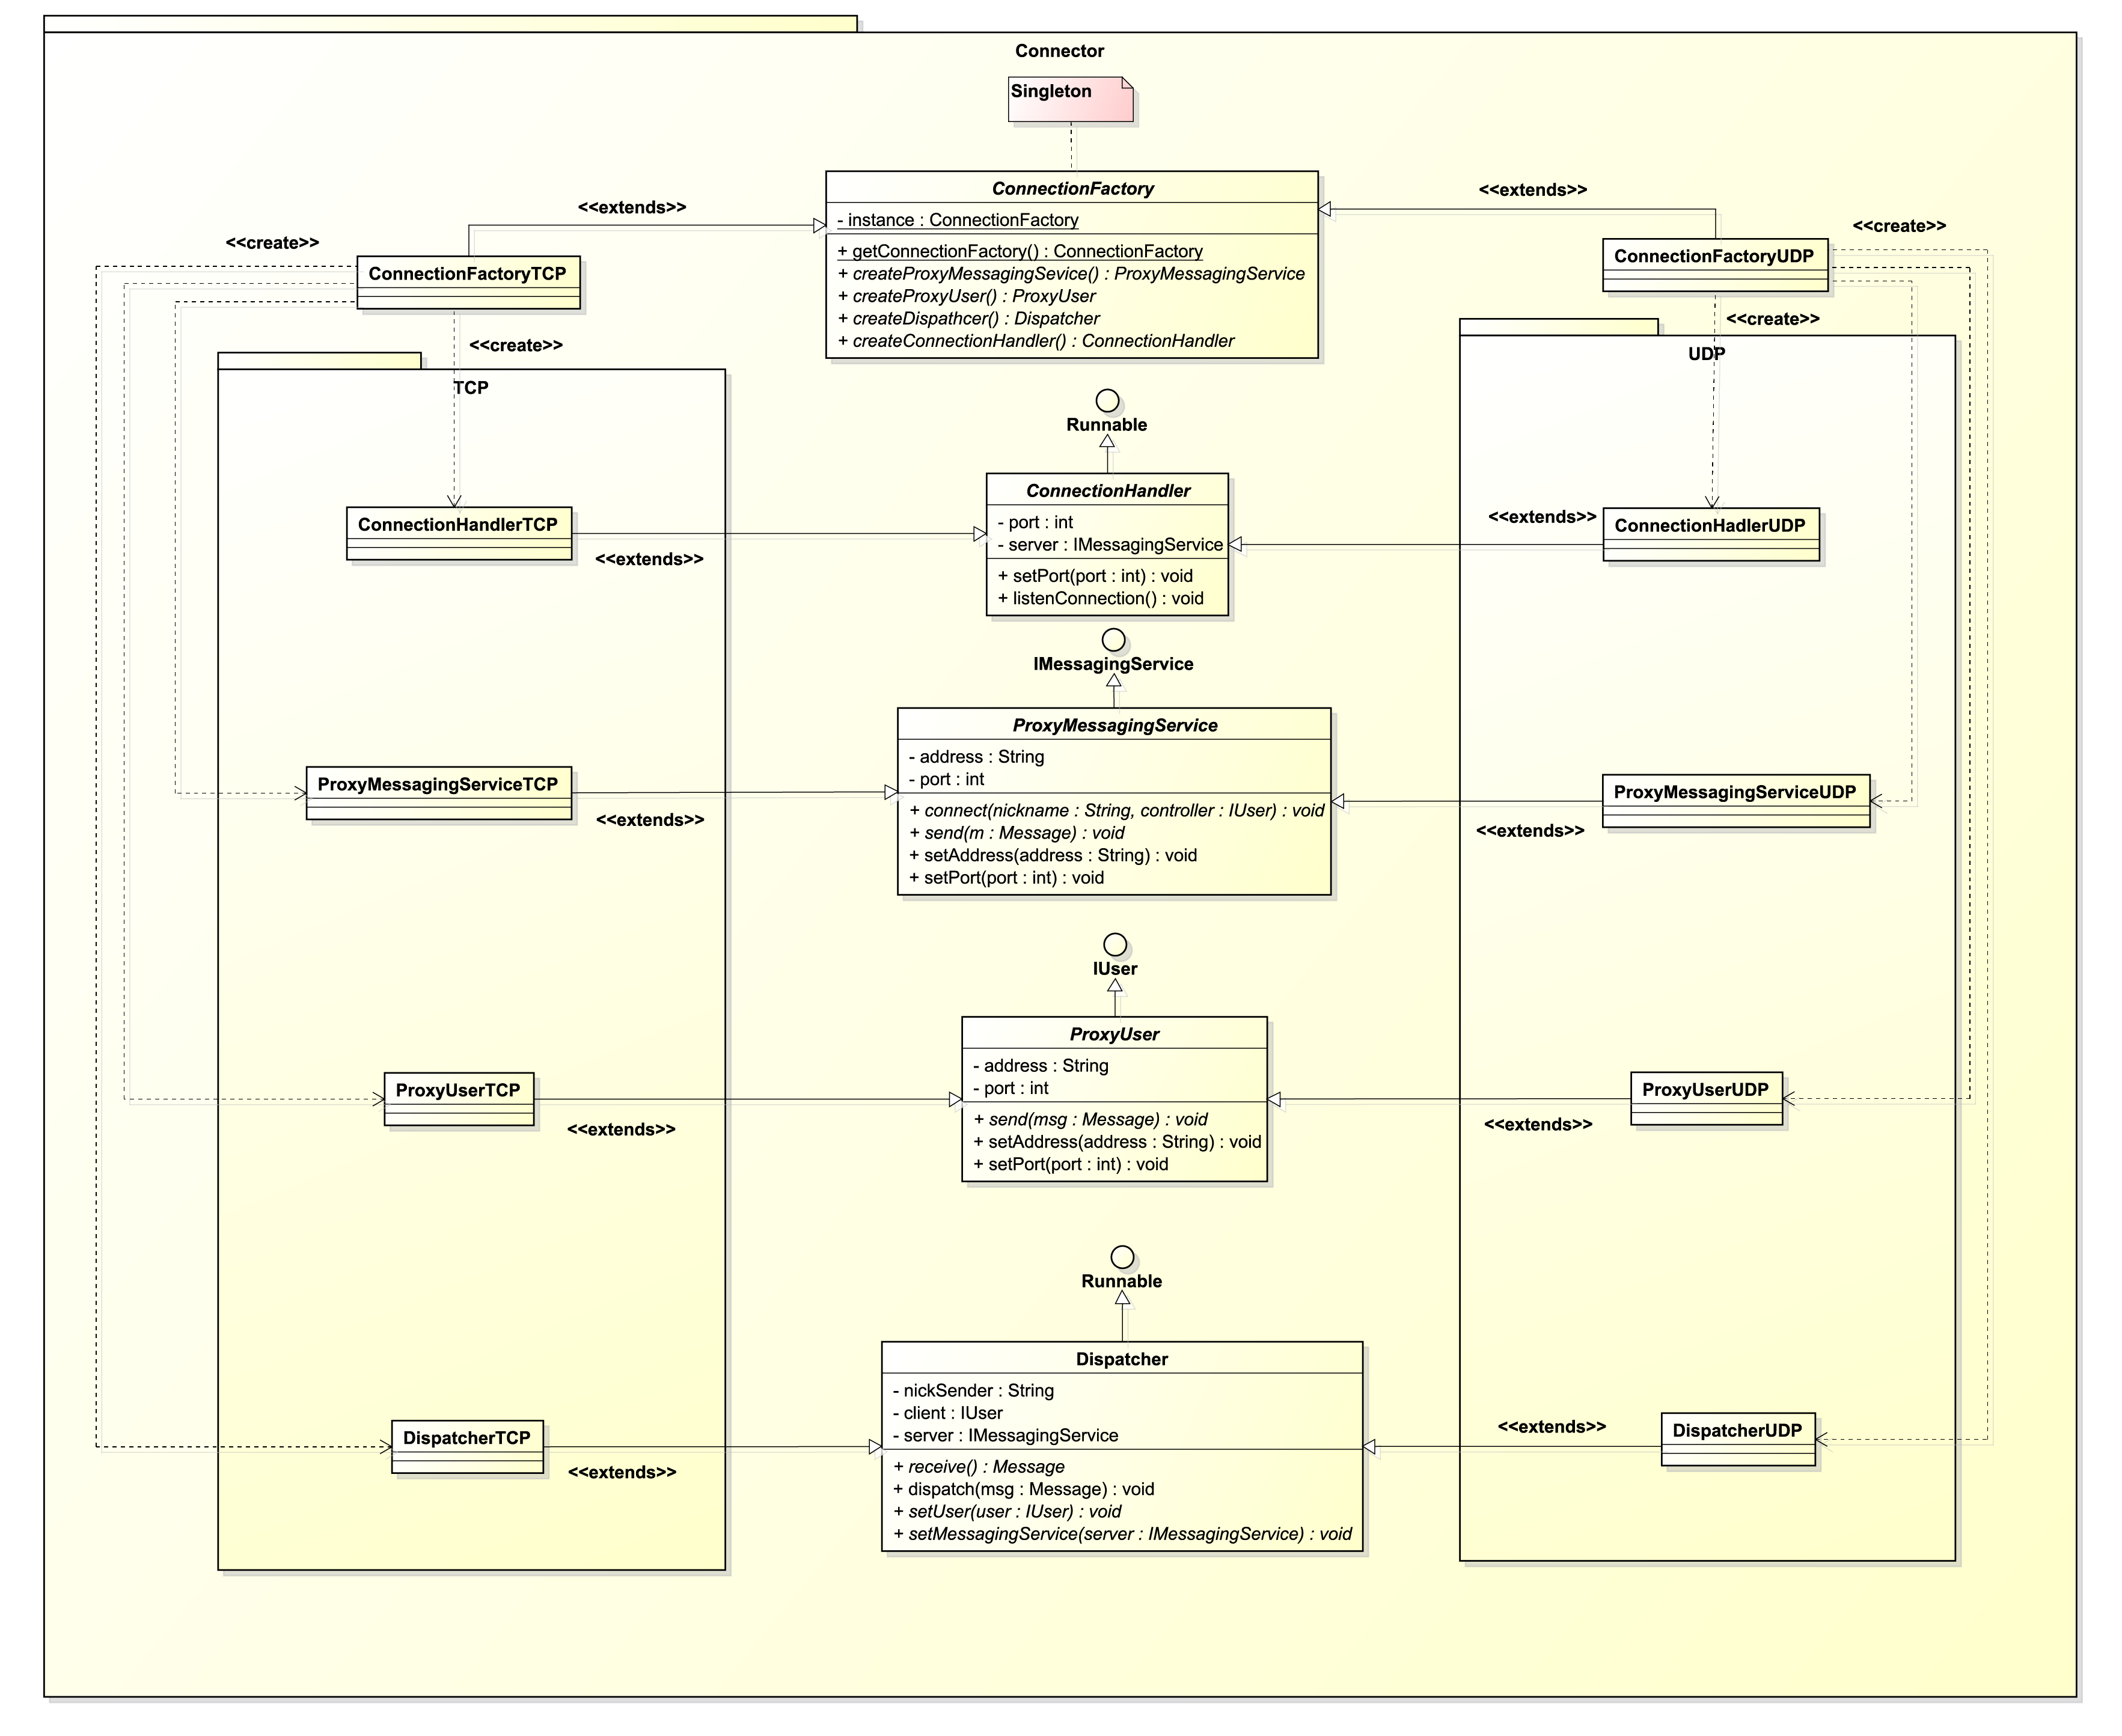
\includegraphics[scale=0.084]{image_astah/Iteration_1_DesignModel_Refactored/ClassDiagramConnector.png}{\centering}
     \caption{DCD - Diagramma delle Classi: Package Connector }
     \label{fig_UC1_UC2_DCDR_3} 
   \end{figure}
\end{frame}

\begin{frame} {Refactoring Iterazione 1: Class Diagram Snuc Server UC1 e UC2}
   \begin{figure}
     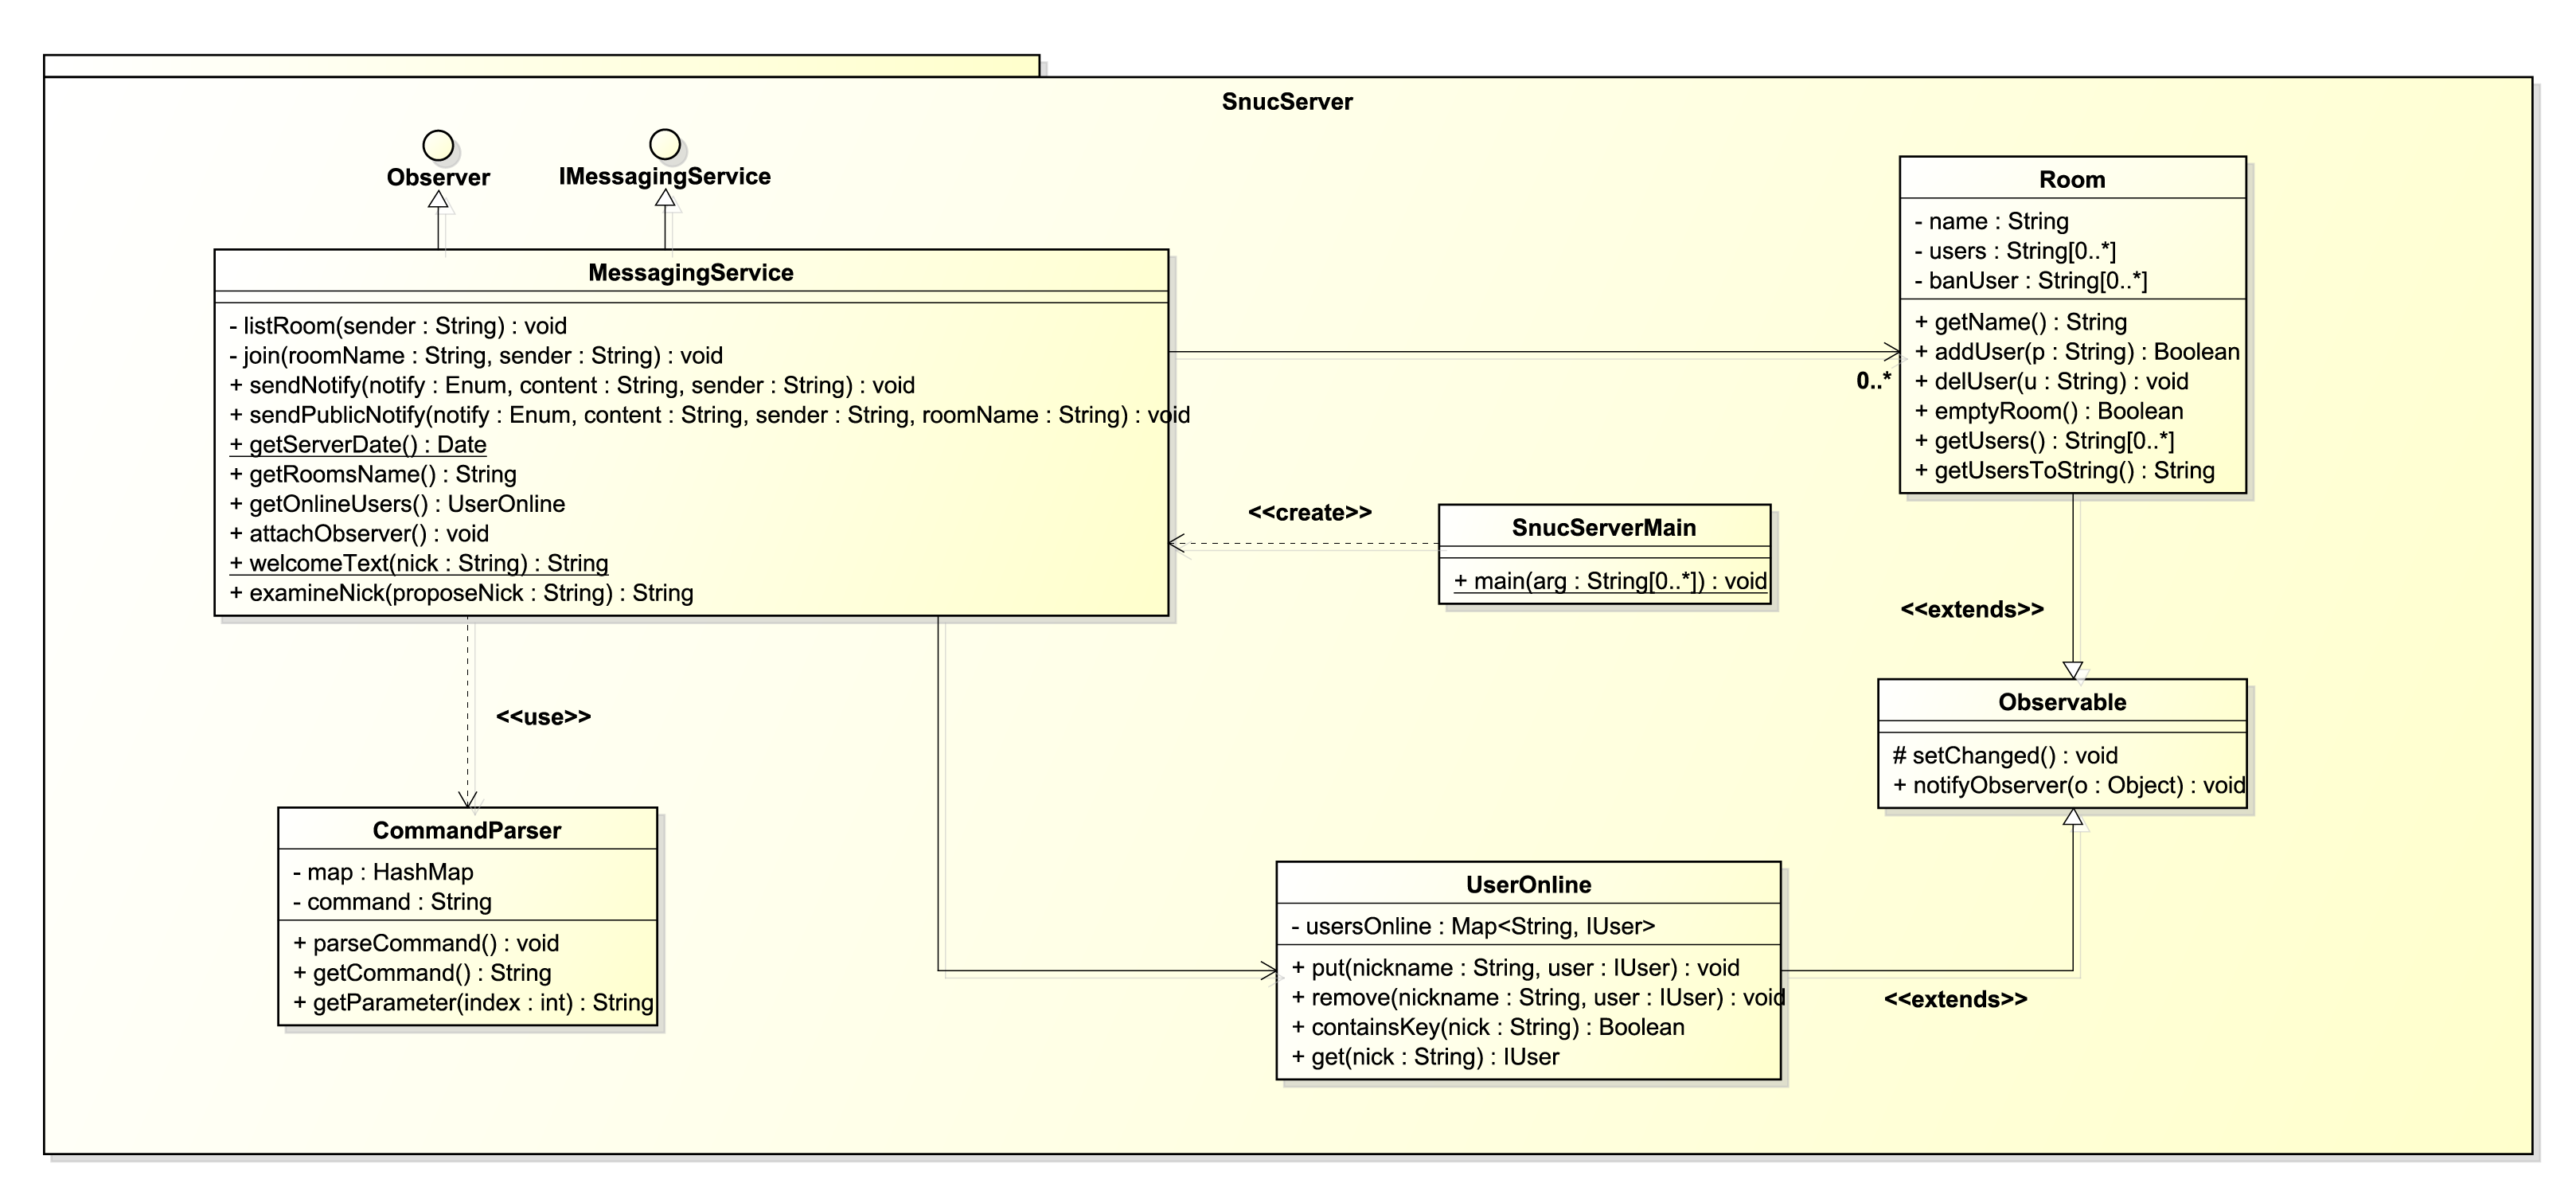
\includegraphics[scale=0.144]{image_astah/Iteration_1_DesignModel_Refactored/ClassDiagramSnucServer.png}{\centering}
     \caption{DCD - Diagramma delle Classi: Package Snuc Server }
     \label{fig_UC1_UC2_DCDR_4} 
   \end{figure}
\end{frame}

\subsection{Refactoring Iterazione 1: SSD UC1 e UC2}
\begin{frame} {Refactoring Iterazione 1: UC1\_RequestConnection}
   \begin{figure}
     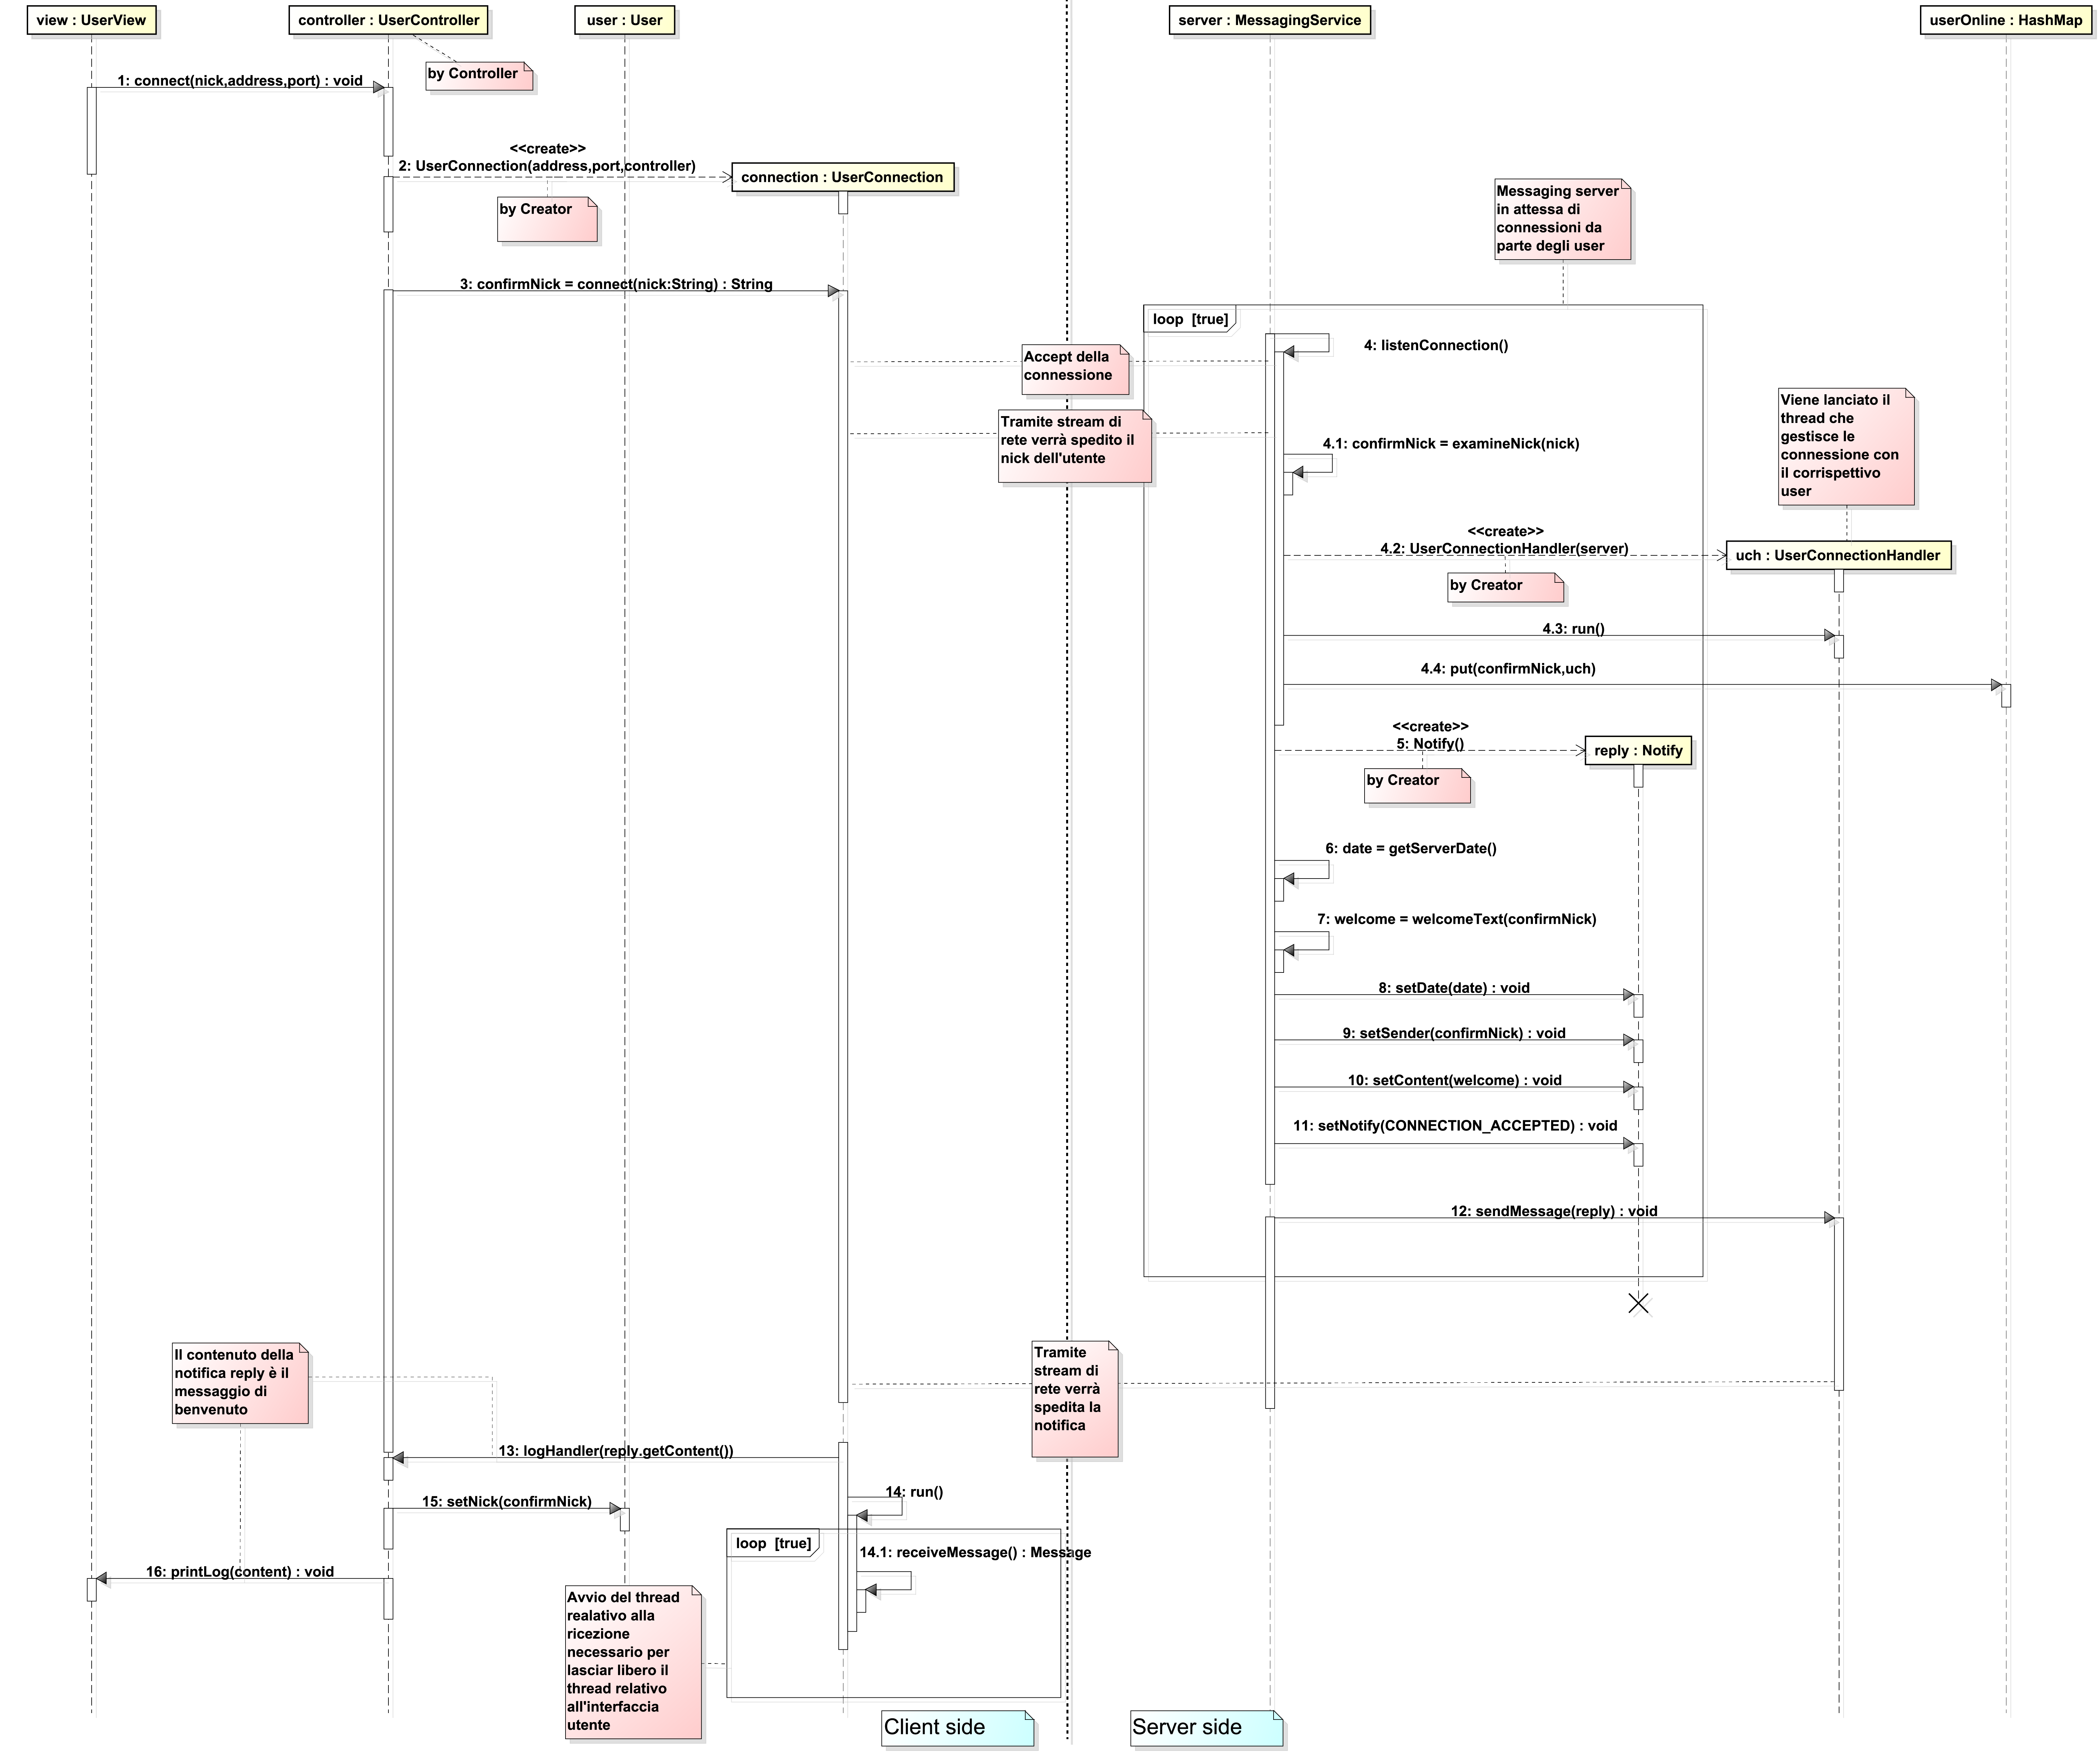
\includegraphics[scale=0.0475]{image_astah/Iteration_1_DesignModel_Refactored/UC1_RequestConnection_SSD_3_4_connect.png}{\centering}
     \caption{SSD - OP1-4: connect(nick), notify(response) del modello dominio (figura \ref{fig_UC1_RC_SSD}) }
     \label{fig_UC1_SSDR_RC_1_4} 
   \end{figure}
\end{frame}

\begin{frame} {Refactoring Iterazione 1: UC2\_AccessRoom - OP1}
   \begin{figure}
     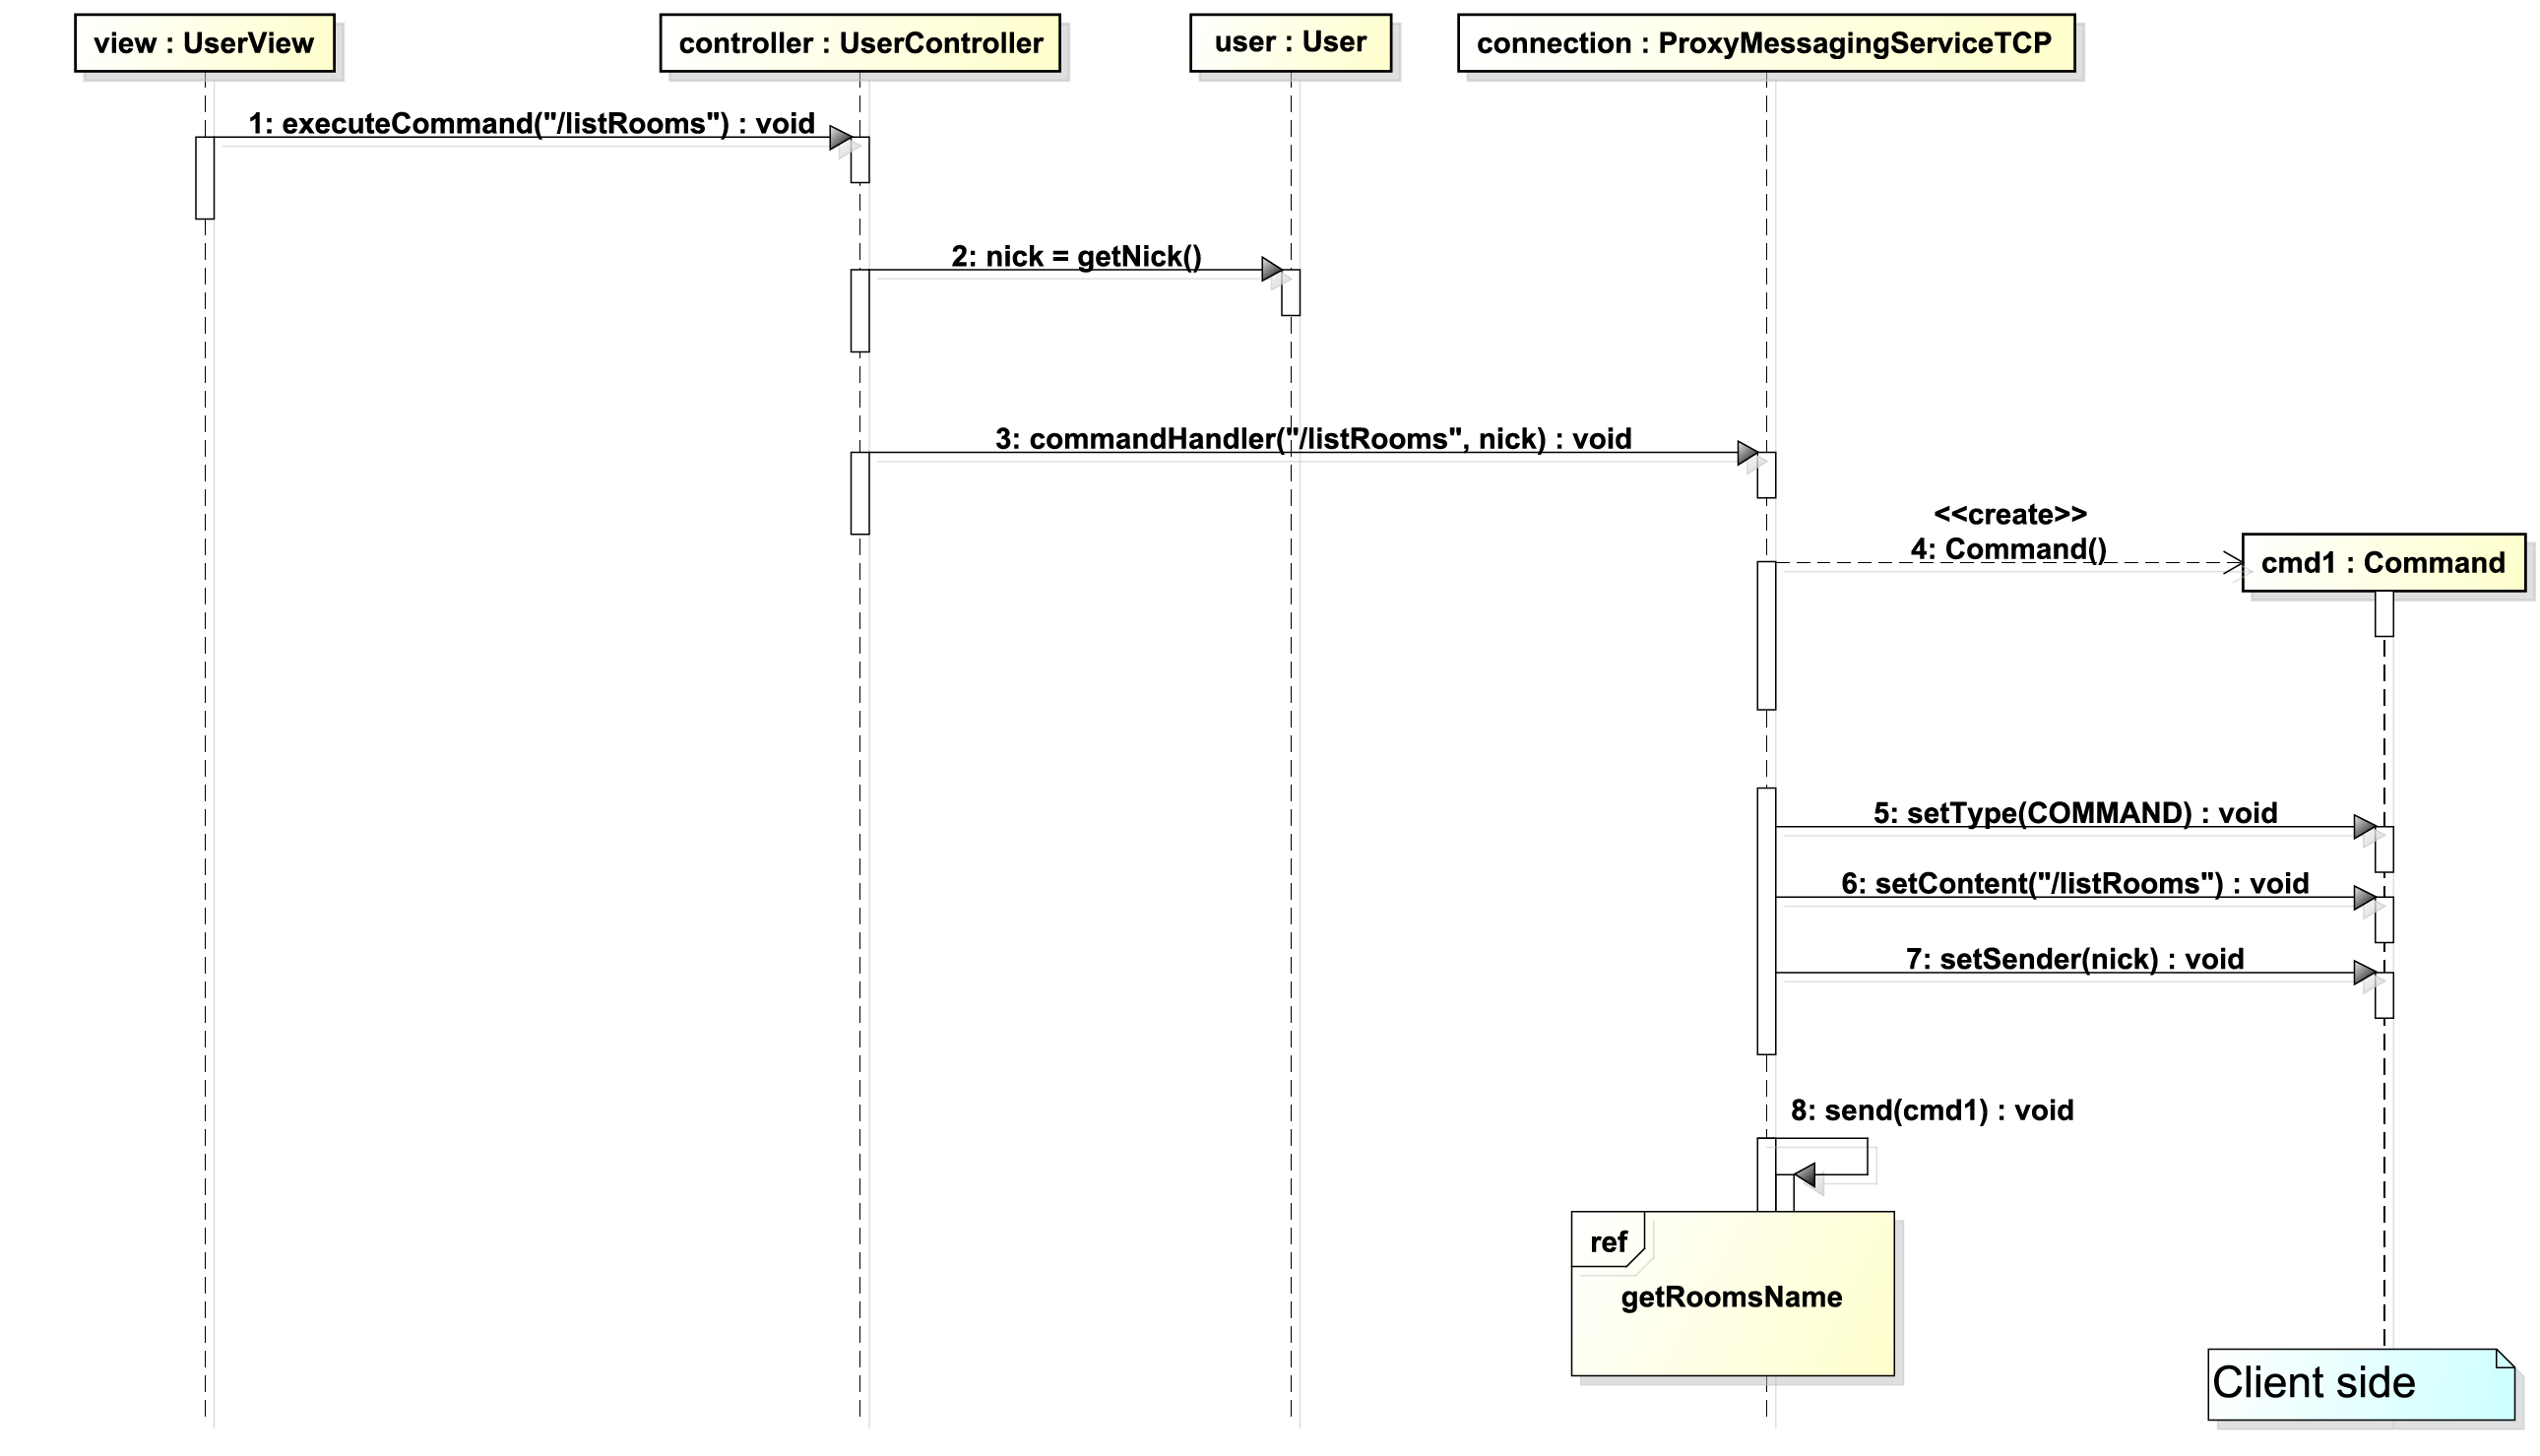
\includegraphics[scale=0.16]{image_astah/Iteration_1_DesignModel_Refactored/UC2_AccessRoom_SSD_1_sendCommand.png}{\centering}
     \caption{SSD - OP1: sendCommand(cmd1) del modello di dominio (figura \ref{fig_UC2_AR_SSD}) }
     \label{fig_UC2_SSDR_AC_1} 
   \end{figure}
\end{frame}

\begin{frame} {Refactoring Iterazione 1: UC2\_AccessRoom - OP2}
   \begin{figure}
     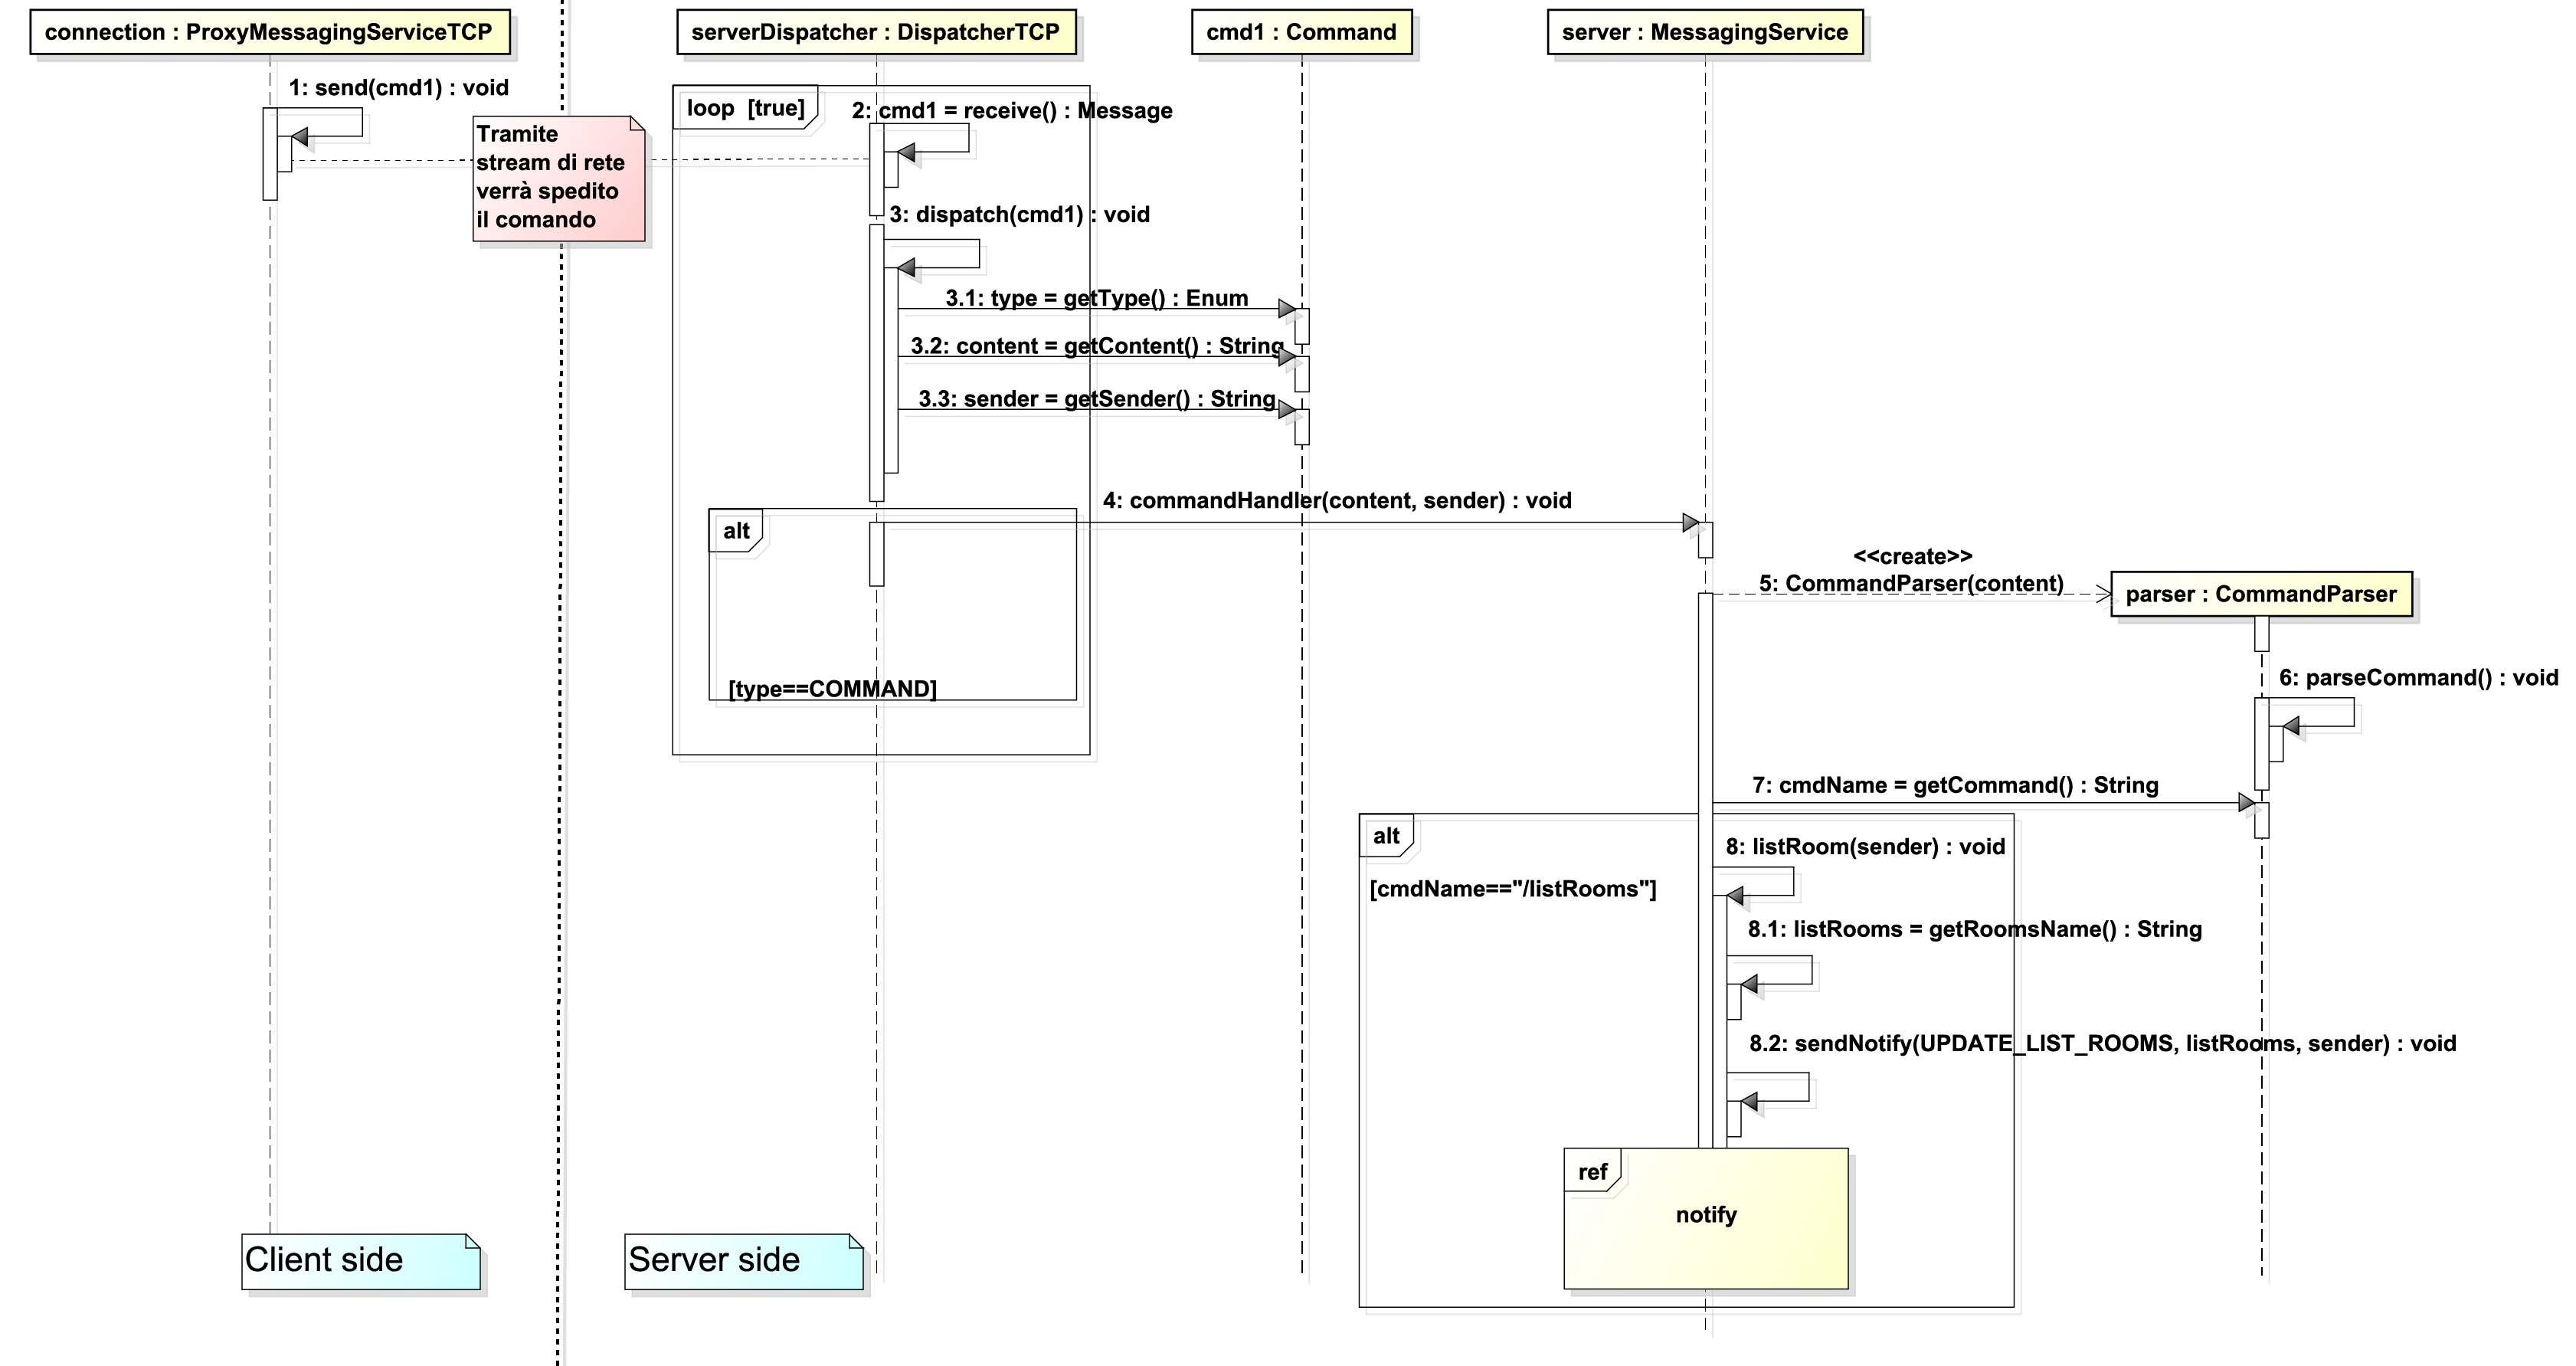
\includegraphics[scale=0.135]{image_astah/Iteration_1_DesignModel_Refactored/UC2_AccessRoom_SSD_2_getRoomsName.png}{\centering}
     \caption{SSD - OP2: getRoomsName() del modello di dominio (figura \ref{fig_UC2_AR_SSD}) }
     \label{fig_UC2_SSDR_AC_2} 
   \end{figure}
\end{frame}

\begin{frame} {Refactoring Iterazione 1: UC2\_AccessRoom - OP3}
   \begin{figure}
     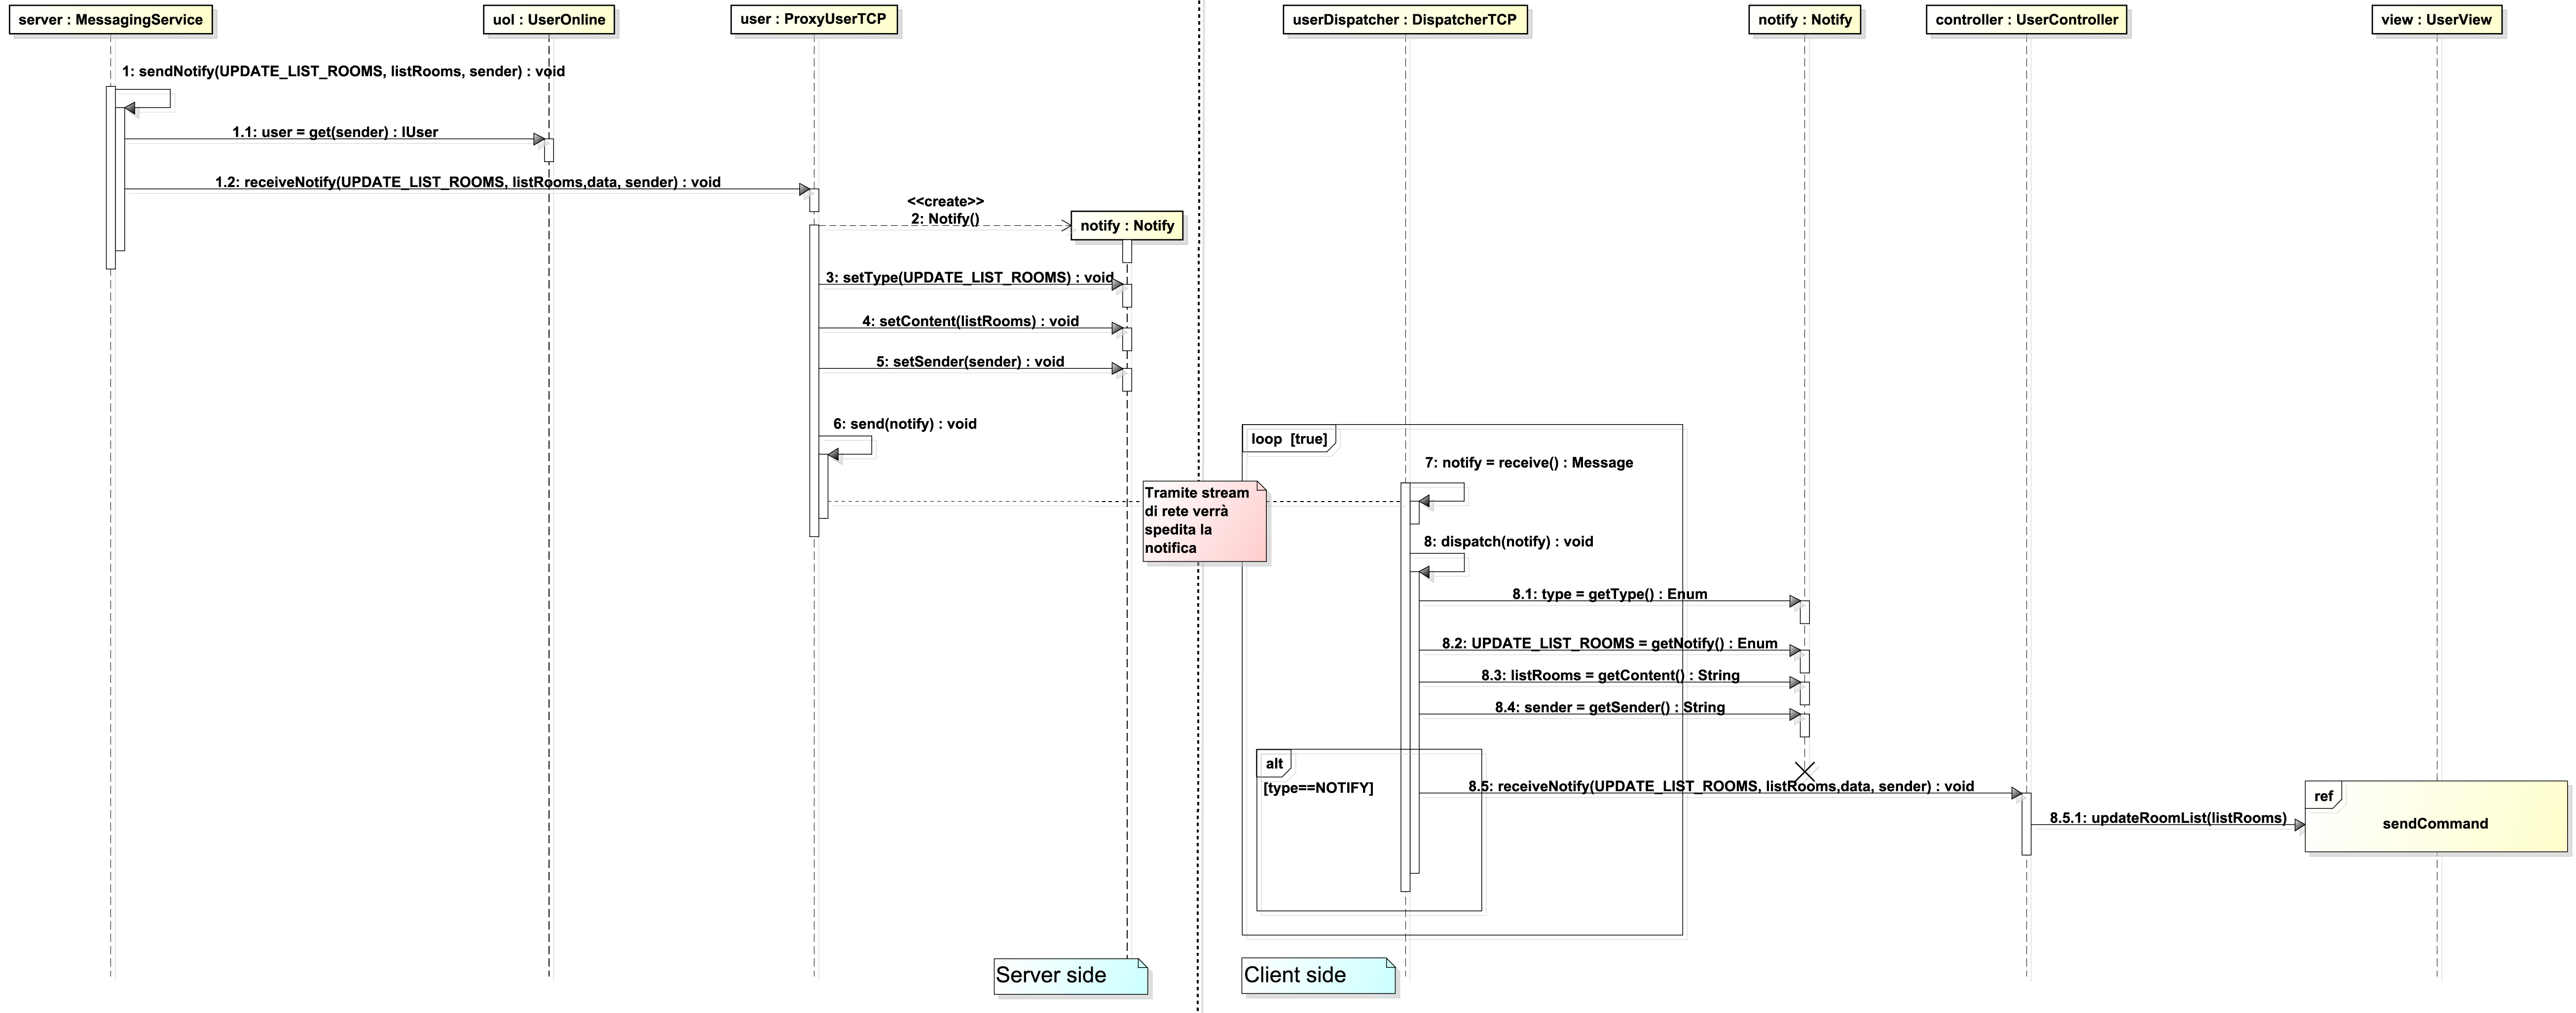
\includegraphics[scale=0.085]{image_astah/Iteration_1_DesignModel_Refactored/UC2_AccessRoom_SSD_3_notify.png}{\centering}
     \caption{SSD - OP3: notify(list) del modello di dominio (figura \ref{fig_UC2_AR_SSD})}
     \label{fig_UC2_SSDR_AC_3} 
   \end{figure}
\end{frame}

\begin{frame} {Refactoring Iterazione 1: UC2\_AccessRoom - OP4}
   \begin{figure}
     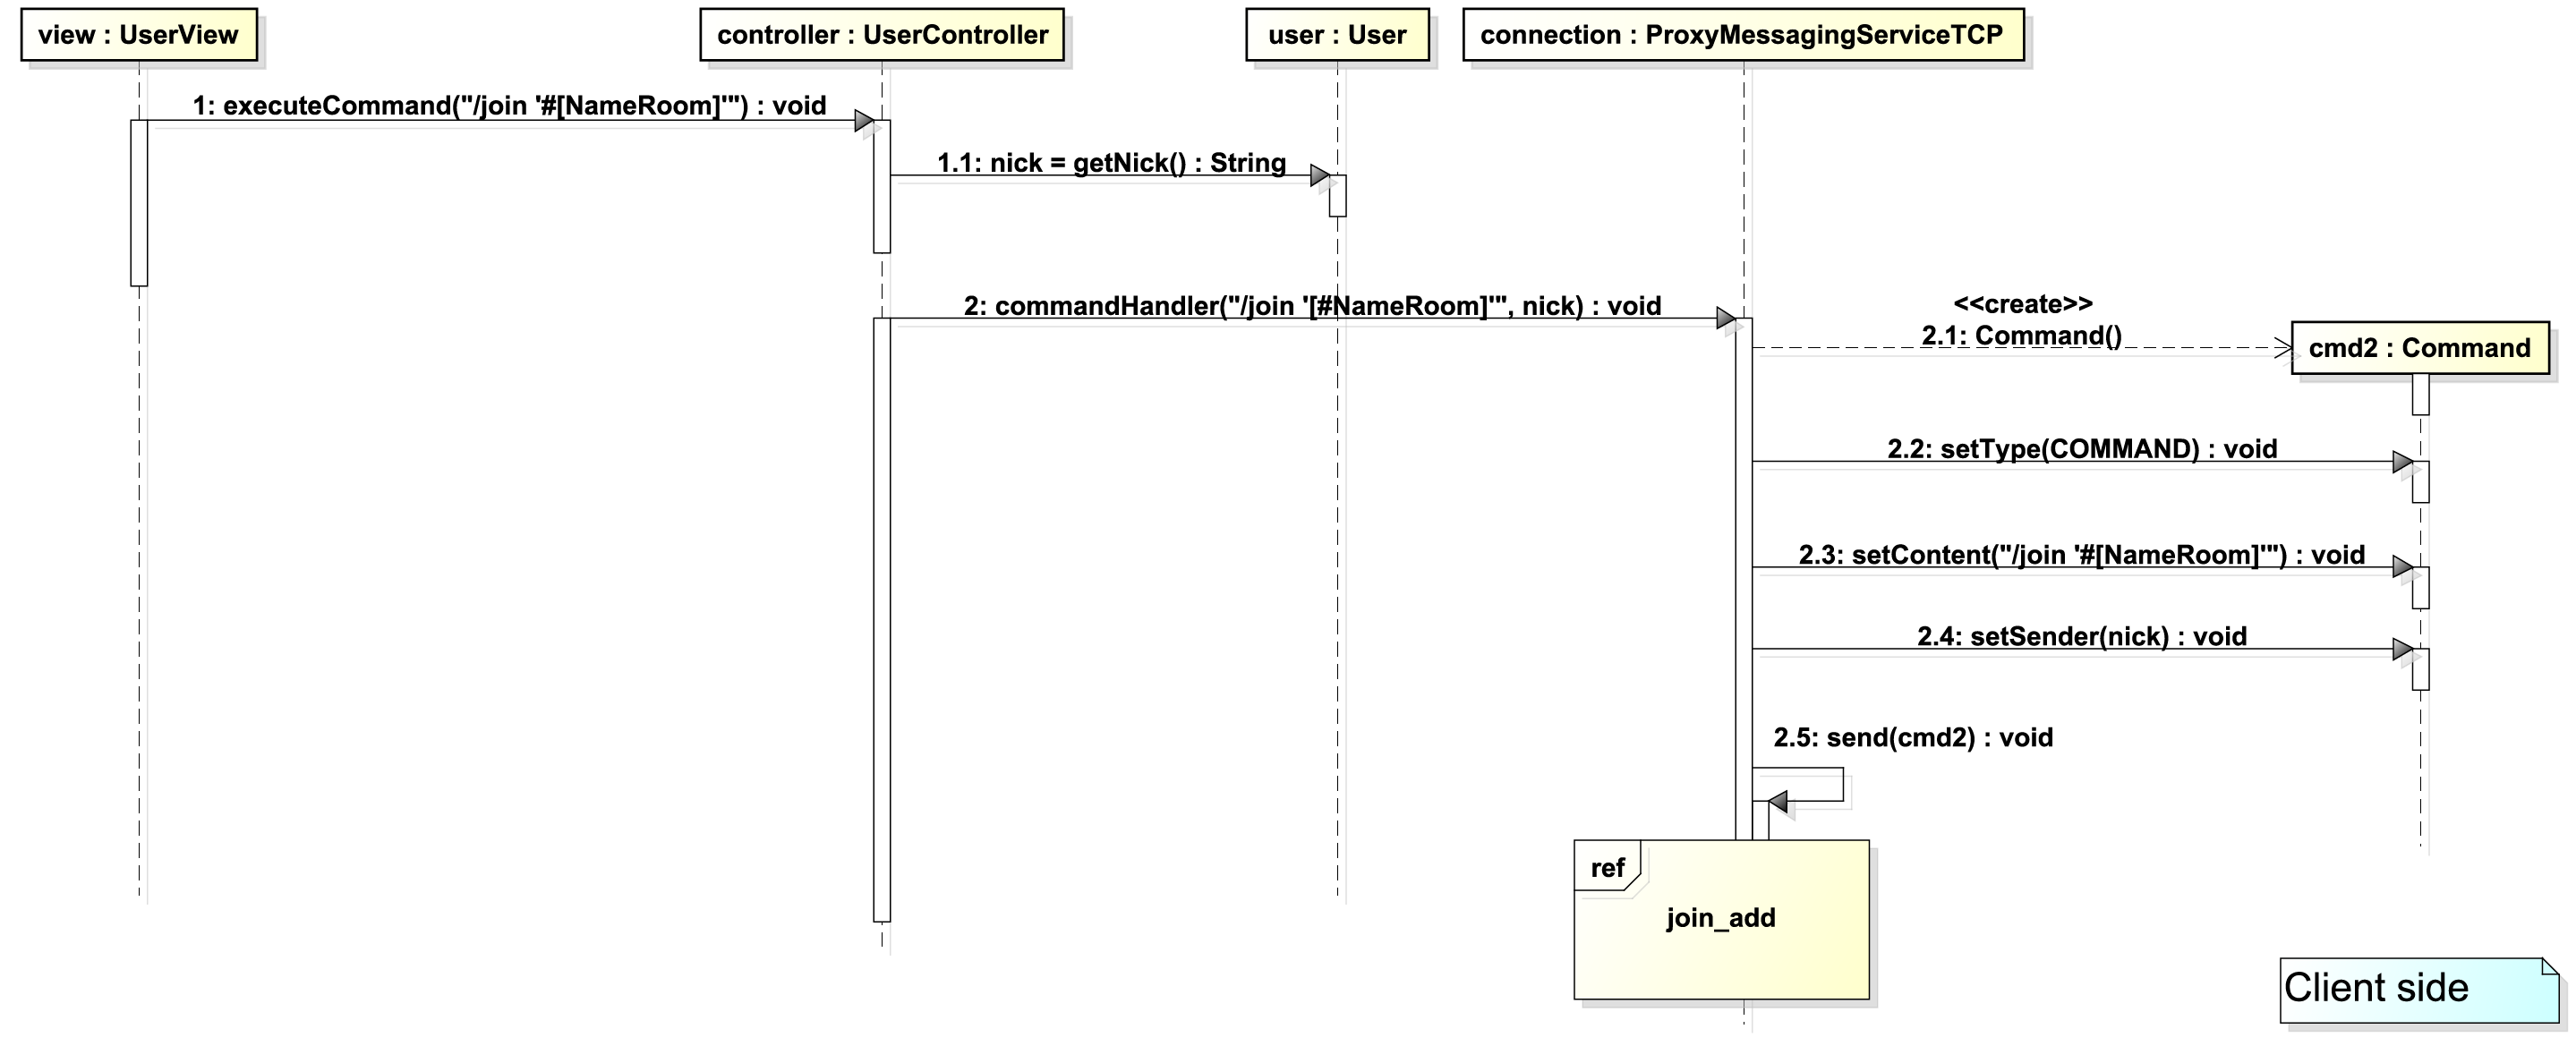
\includegraphics[scale=0.158]{image_astah/Iteration_1_DesignModel_Refactored/UC2_AccessRoom_SSD_4_sendCommand.png}{\centering}
     \caption{SSD - OP4: sendCommand(cmd2) del modello di dominio (figura \ref{fig_UC2_AR_SSD}) }
     \label{fig_UC2_SSDR_AC_4} 
   \end{figure}
\end{frame}

\begin{frame} {Refactoring Iterazione 1: UC2\_AccessRoom - OP5}
   \begin{figure}
     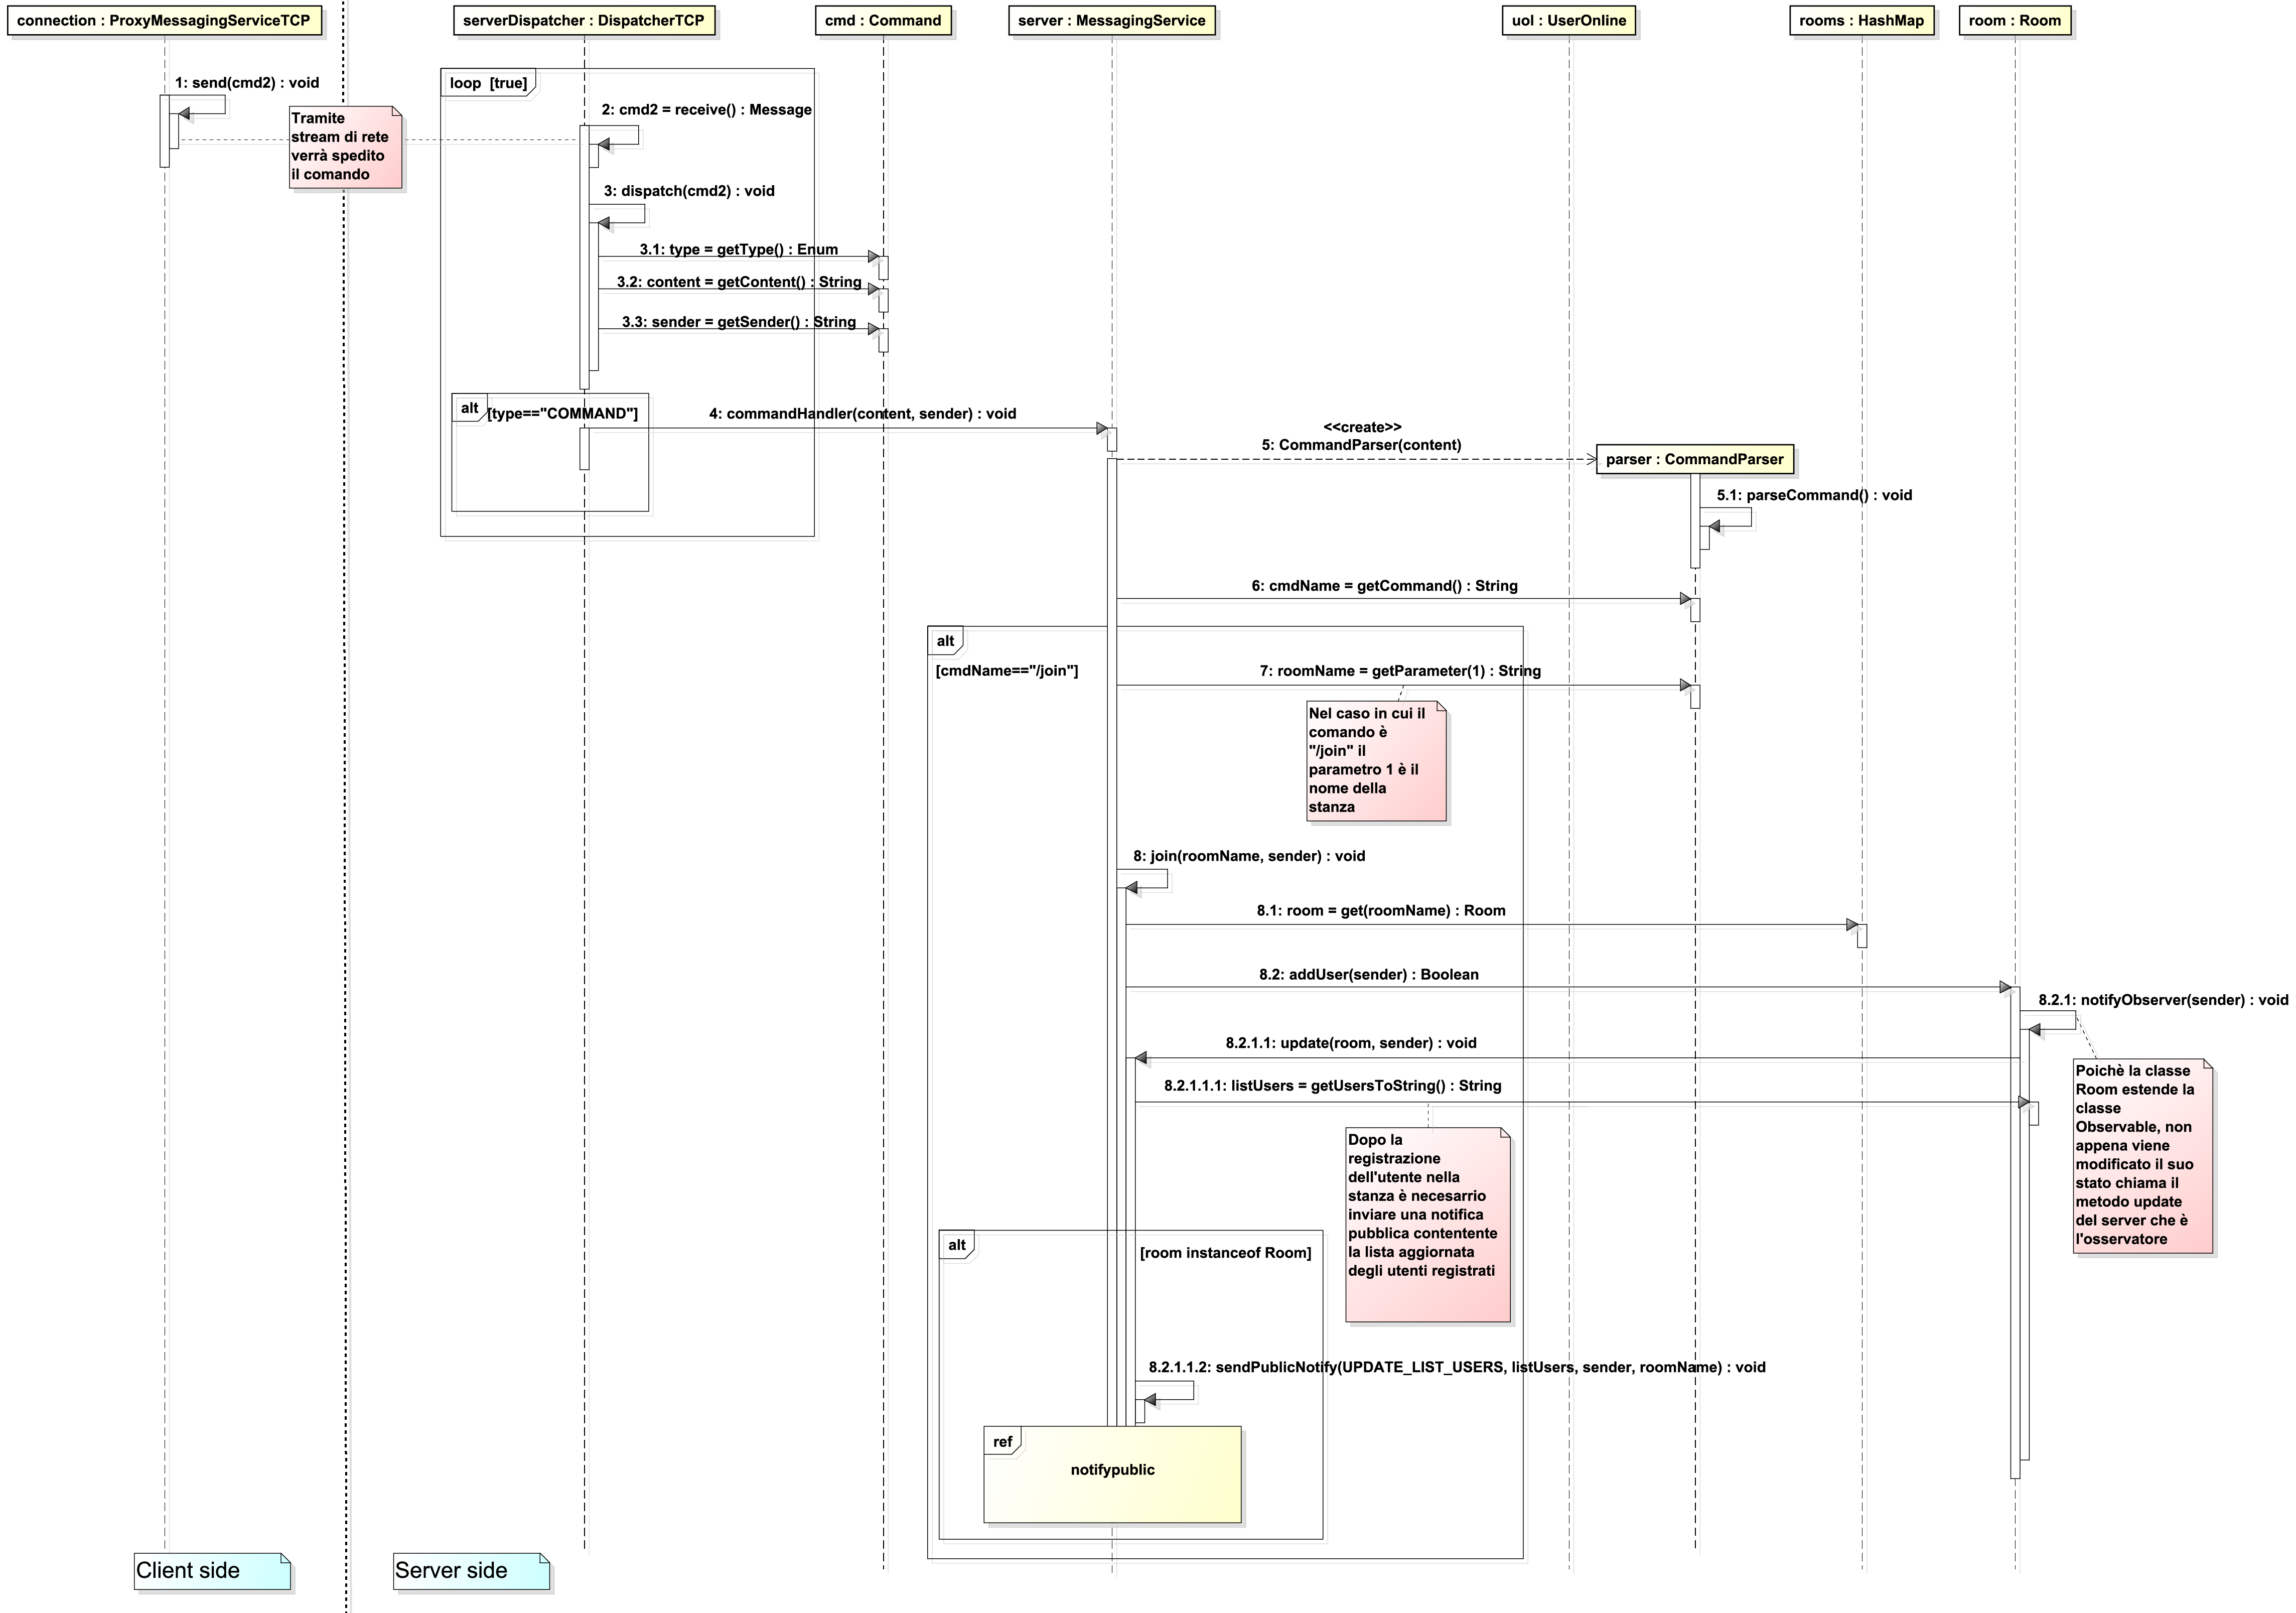
\includegraphics[scale=0.075]{image_astah/Iteration_1_DesignModel_Refactored/UC2_AccessRoom_SSD_5_join_add.png}{\centering}
     \caption{SSD - OP5: joinRoom(sender,room), addUserToRoom() del modello di dominio (figura \ref{fig_UC2_AR_SSD}) }
     \label{fig_UC2_SSDR_AC_5} 
   \end{figure}
\end{frame}

\begin{frame} {Refactoring Iterazione 1: UC2\_AccessRoom - OP6}
   \begin{figure}
     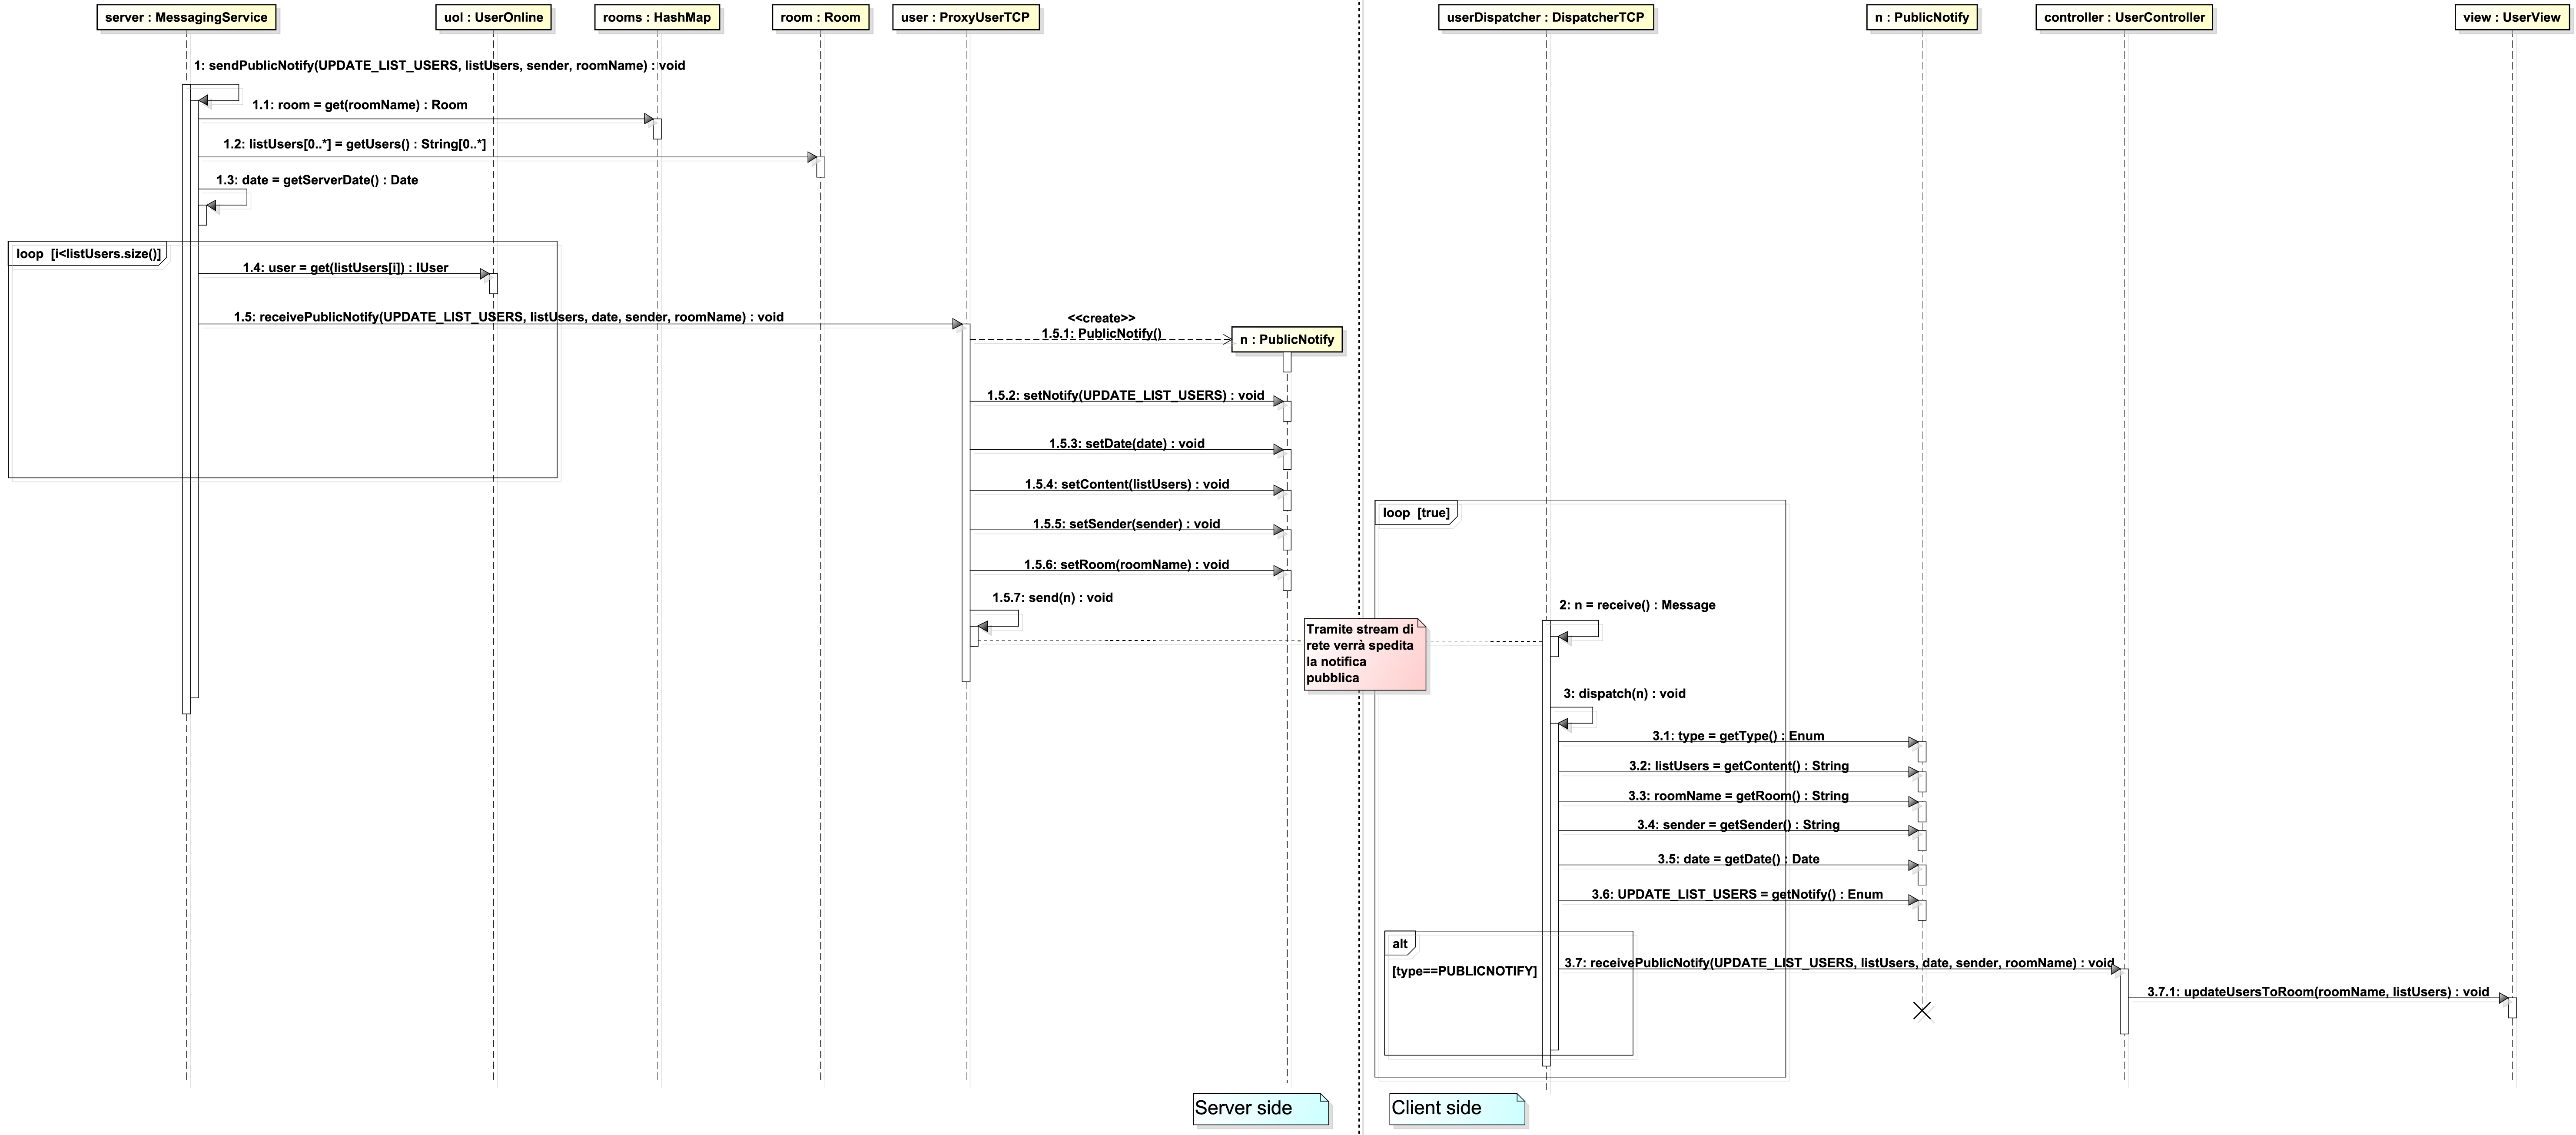
\includegraphics[scale=0.077]{image_astah/Iteration_1_DesignModel_Refactored/UC2_AccessRoom_SSD_6_notifypublic.png}{\centering}
     \caption{SSD - OP6: notifypublic(updateList) del modello di dominio (figura \ref{fig_UC2_AR_SSD}) }
     \label{fig_UC2_SSDR_AC_6} 
   \end{figure}
\end{frame}

\subsection{Refactoring Iterazione 1: Implementazione UC1 e UC2}
\begin{frame} {Refactoring Iterazione 1: Implementazione UC1 e UC2}
 \emph{INSERIRE DESCRIZIONE}
\end{frame}

\subsection {Refactoring Iterazione 1: Test UC1 e UC2}
\begin{frame}[allowframebreaks] {Refactoring Iterazione 1: Test UC1 e UC2}
 \emph{INSERIRE ESEMPI DEI TEST EFFETTUATI}
   \lstinputlisting[caption=sample,language=java]{example.java}
\end{frame}

% ELABORAZIONE ITERAZIONE 2 - UC3_SendPublicMessage
\section{Elaborazione - Iterazione 2}
\begin{frame} {Descrizione Elaborazione - Iterazione 2}
  \emph{INSERIRE DESCRIZIONE}
\end{frame}

\subsection{Iterazione 2: Requisiti - UC3\_SendPublicMessage}
\begin{frame} {Iterazione 2: Requisiti - UC3\_SendPublicMessage}
  \begin{table}[!htbp]
    \caption {Caso d'uso UC3\_SendPublicMessage}
     \label{table_UC3_SPM}
      \resizebox{\linewidth}{!}{%
       \begin{tabular}{|l|p{10cm}|}\hline
        Nome caso d'uso &  UC3\_SendPublicMessage\\\hline
        Portata & Applicazione Smart Intelligent University Communications \\\hline
        Livello & Obiettivo Utente \\\hline
        Attore primario & SnucUser  \\\hline
        Parti interessate e interessi & 
         \begin{itemize}
          \item SnucUser, vuole che i messaggi siano inviati a ogni utente della stanza virtuale.
          \item SnucAdmin, è interessato a supervisionare gli utenti del servizio affinché non ci siano abusi.       
         \end{itemize} \\\hline
        Pre-condizioni &  L'utente è registrato nella stanza in cui desidera inviare i messaggi.\\\hline
        Post-condizioni (garanzia di successo) & Ogni utente riceve il messaggio inviato. \\\hline
         Scenario principale di successo &  
         \begin{enumerate} 
          \item L’utente inserisce in una opportuna area il messaggio da inviare.
          \item Il messaggio viene inoltrato agli utenti presenti nella stanza selezionata. 
         \end{enumerate} \\\hline
      \end{tabular}}
   \end{table}
\end{frame}

\begin{frame} {Iterazione 2: Requisiti - UC3\_SendPublicMessage}
  \begin{table}[!htbp]
      \resizebox{\linewidth}{!}{%
       \begin{tabular}{|l|p{10cm}|}\hline
         Requisiti speciali (Requisiti Non Funzionali) &  Comunicazione asincrona in cui lo scambio di informazioni avviene in tempo reale, senza sensibili pause tra 
                                                        invio e ricezione del messaggio\\\hline
         Elenco delle varianti tecnologiche &  
          \begin{itemize}  
           \item \`E possibile inviare messaggi confidenziali, autenticati e integri al server del servizio di messaggistica.
           \item L’applicazione dovrebbe essere flessibile al funzionamento di diversi protocolli di comunicazione (es. TCP, UDP) e con diversi strati middleware 
                 (es. Socket, RMI)
          \end{itemize} \\\hline
         Frequenza di ripetizione & Potrebbe essere quasi ininterrotta \\\hline
         Varie e/o Problemi Aperti &  // \\\hline
      \end{tabular}}
   \end{table}
\end{frame}

\subsection {Iterazione 2: Analisi - UC3\_SendPublicMessage}
\begin{frame} [allowframebreaks] {Descrizione Iterazione 2: Analisi - UC3\_SendPublicMessage}
  In questa iterazione, del caso d’uso UC3 è di interesse lo scenario principale di successo.  Da esso è possibile identificare le seguenti classi concettuali: 
  \begin{itemize}
   \item \textbf{User}: rappresenta il generico utente, caratterizzato da un ``nickname'', connesso al servizio di messaggistica. Può richiedere la lista delle 
         stanze, ricevere notifiche dal sistema centrale. Interagisce con il MessagingSevice richiedendo la registrazione e l’ingresso in una specifica stanza. 
         \textit{Può inviare messaggi pubblici agli utenti di una stanza}.
   \item \textbf{MessagingService}: rappresenta ed incapsula il servizio di messaggistica nel suo complesso. Mantiene una lista di utenti connessi a tale sistema. 
          Mantiene una lista di stanze e riceve tramite comandi richieste di ingresso da parte degli utenti. \textit{Svolge il ruolo di smistatore di messaggi 
          inviati dagli User}.
   \item \textbf{Message}: individua un generico messaggio scambiato tra utenti della chat o tra servizio di messaggistica e utente. È costituito da un 
         ``content'' (contenuto del messaggio), da una ``date'' (rappresenta la data) e dal ``sender'' (mittente).
   \item \textbf{Notify}: è una specializzazione del tipo Message ed è caratterizzata da un typeNotify che serve a distinguere il tipo di notifica (ad es. 
          CONNECTIO\_ACCEPT nel caso in cui la connessione è stata stabilita correttamente, BAD\_COMMAND nel caso in cui il comando inviato dall'User non 
          sia riconosciuto dal Server).
    \item \textbf{PublicNotify}: è una specializzazione di Notify e questo tipo di notifica viene ricevuta da tutti gli utenti registrati alla relativa 
          stanza. Un esempio di PublicNotify è la notifica caratterizzata dal seguente typeNotify: UPDATE\_LIST\_USERS, grazie alla quale viene 
          aggiornata la lista degli utenti registrati nella relativa stanza.
   \item  \textbf{Commad}: è una specializzazione di Message e rappresenta il comando che viene inviato dall'User e ricevuto ed interpretato dal            
          MessagingService (es. /join '\#Medical' richiesta da parte dell'utente a registrarsi alla stanza Medical).        
    \item \textbf{Room}: è caratterizzata da un nome. Ciascuna istanza individua una specifica stanza nella chat.
    \item \textbf{Register}: mantiene un riferimento all’insieme di partecipanti che in un certo istante sono presenti nella stanza.
   \item \textit{\textbf{PublicMessage}: è una specializzazione di Message ed individua un messaggio pubblico scambiato tra utenti della chat registrati nella 
         stessa stanza}. 
  \end{itemize}
\end{frame}

\begin{frame} {Iterazione 2: Analisi - UC3\_SendPublicMessage}
   \begin{figure}
     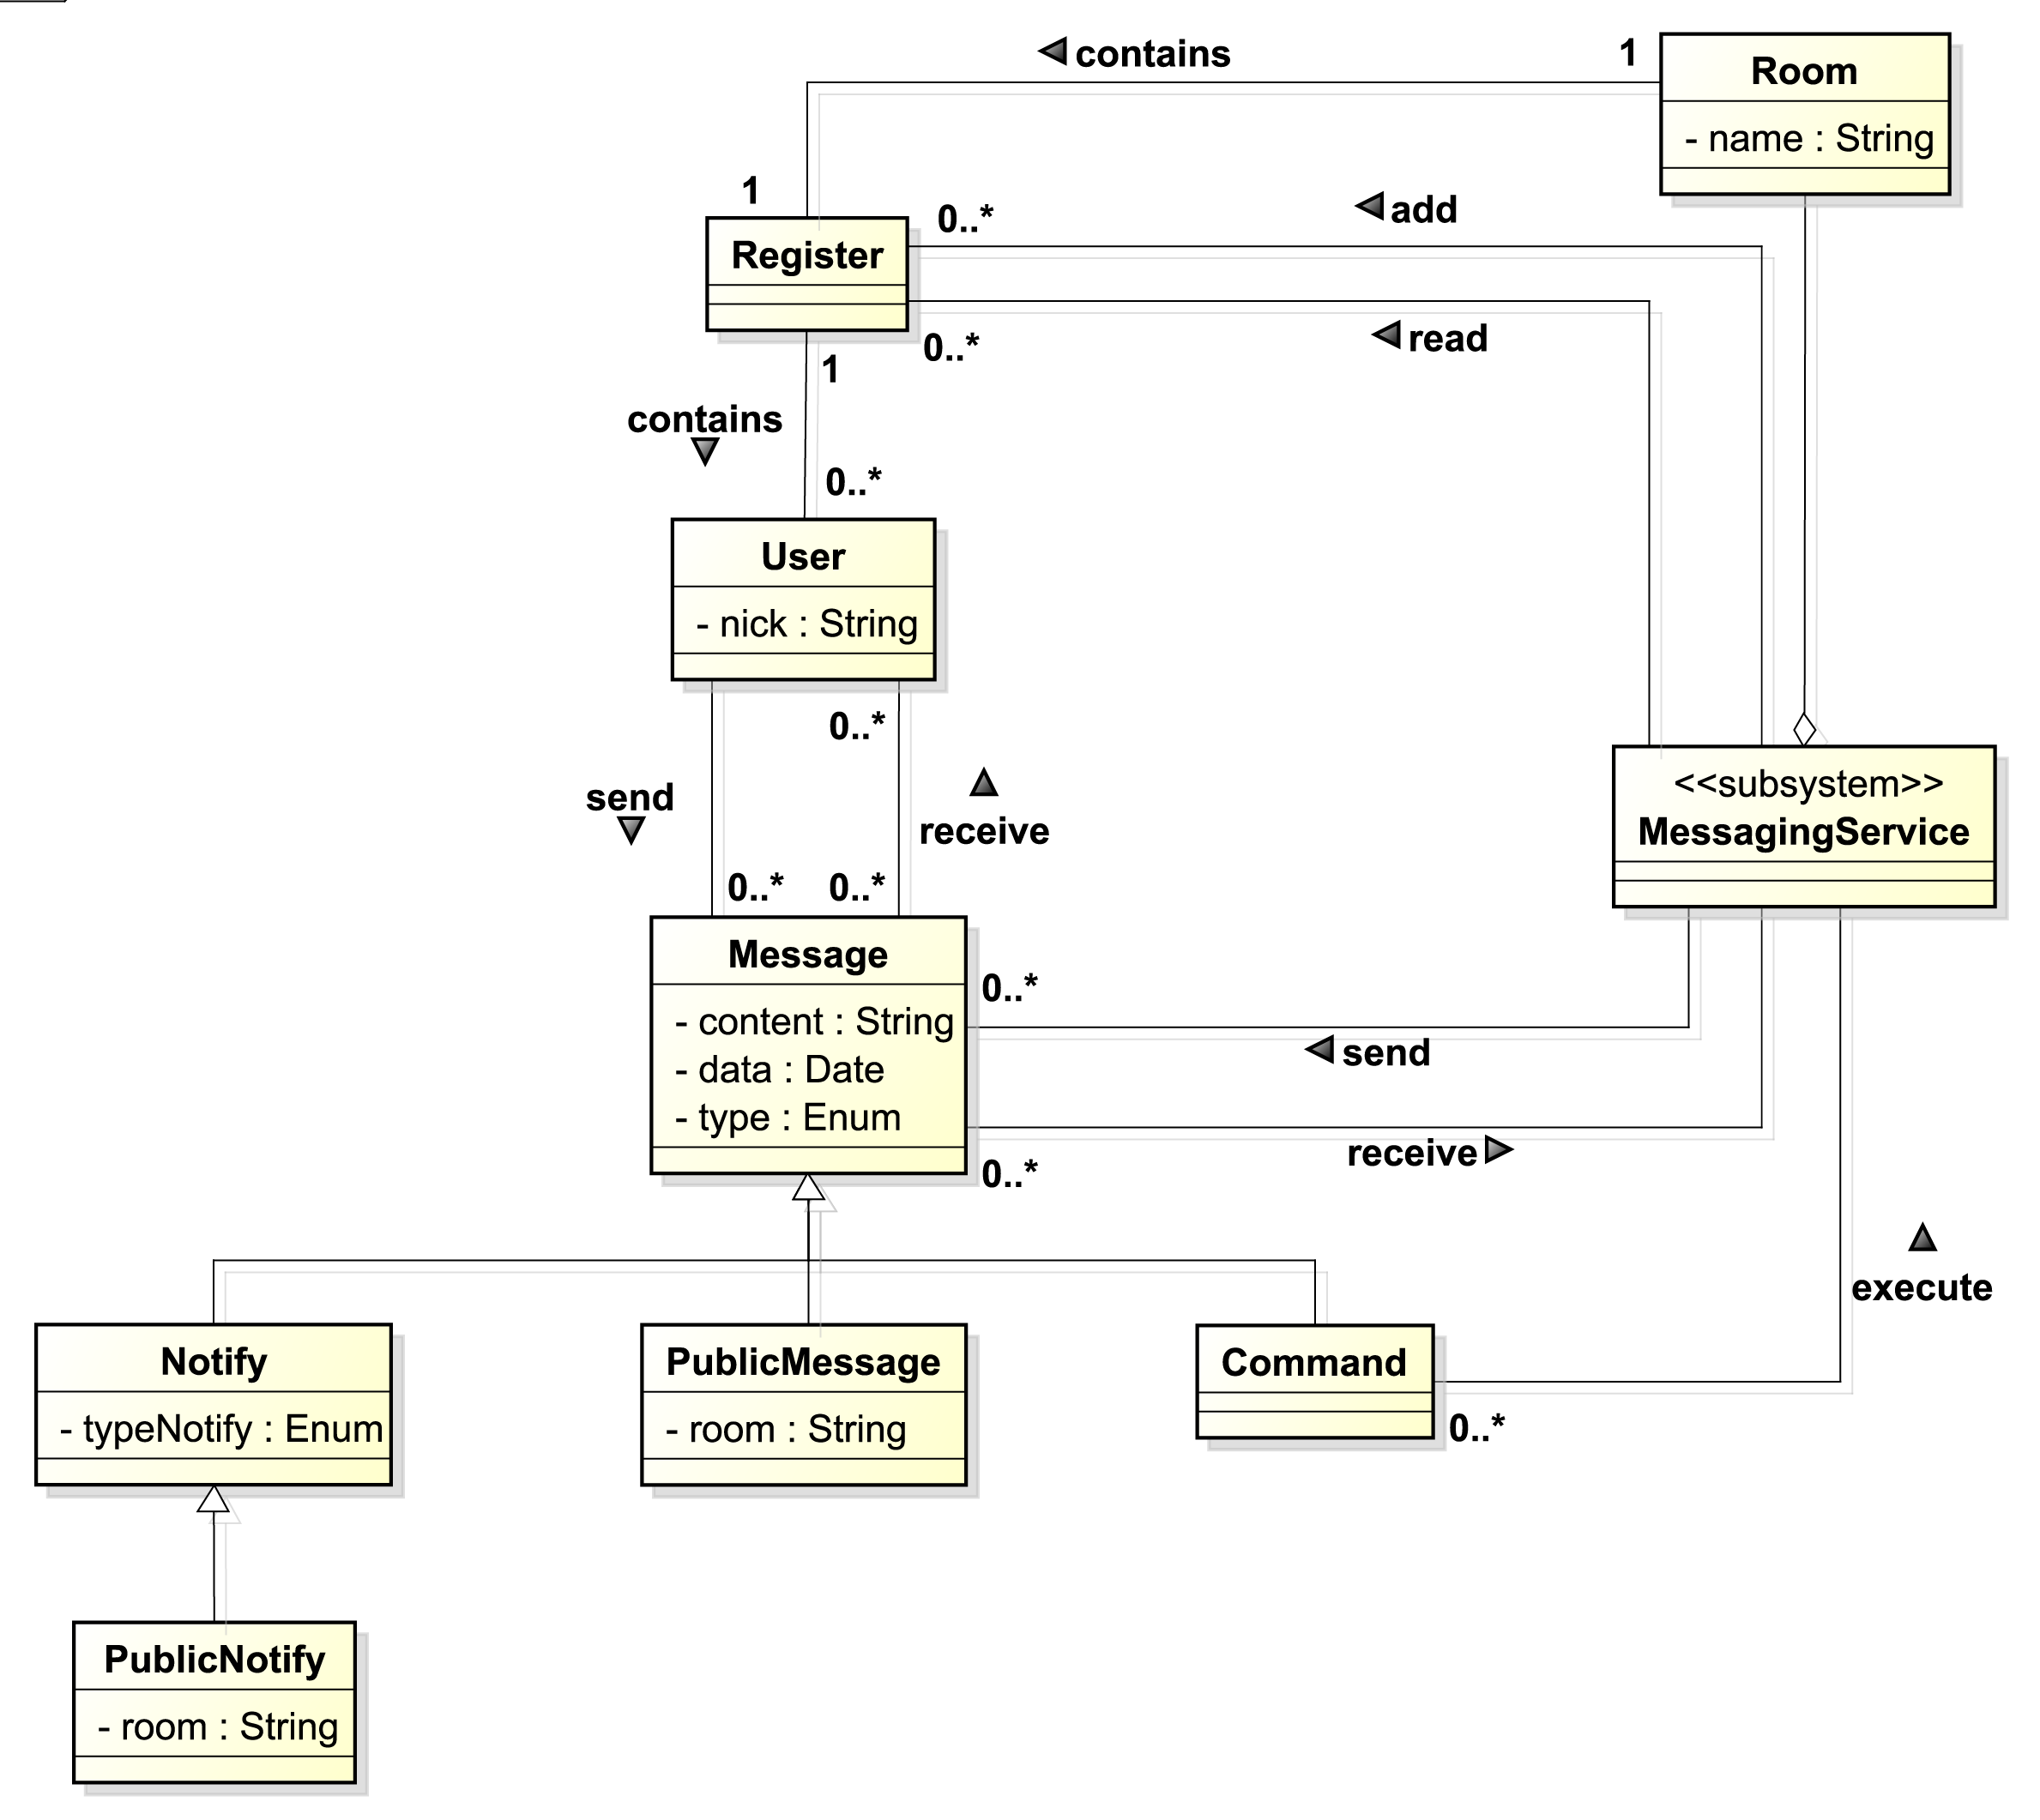
\includegraphics[scale=0.17]{image_astah/Iteration_2_DomainModel/UC3_SendPublicMessage_DM.png}{\centering}
     \caption{UC3 - Modello di dominio}
     \label{fig_UC3_SPM_DM} 
   \end{figure}
\end{frame}

\begin{frame} {Iterazione 2: Analisi - UC3\_SendPublicMessage}
   \begin{figure}
     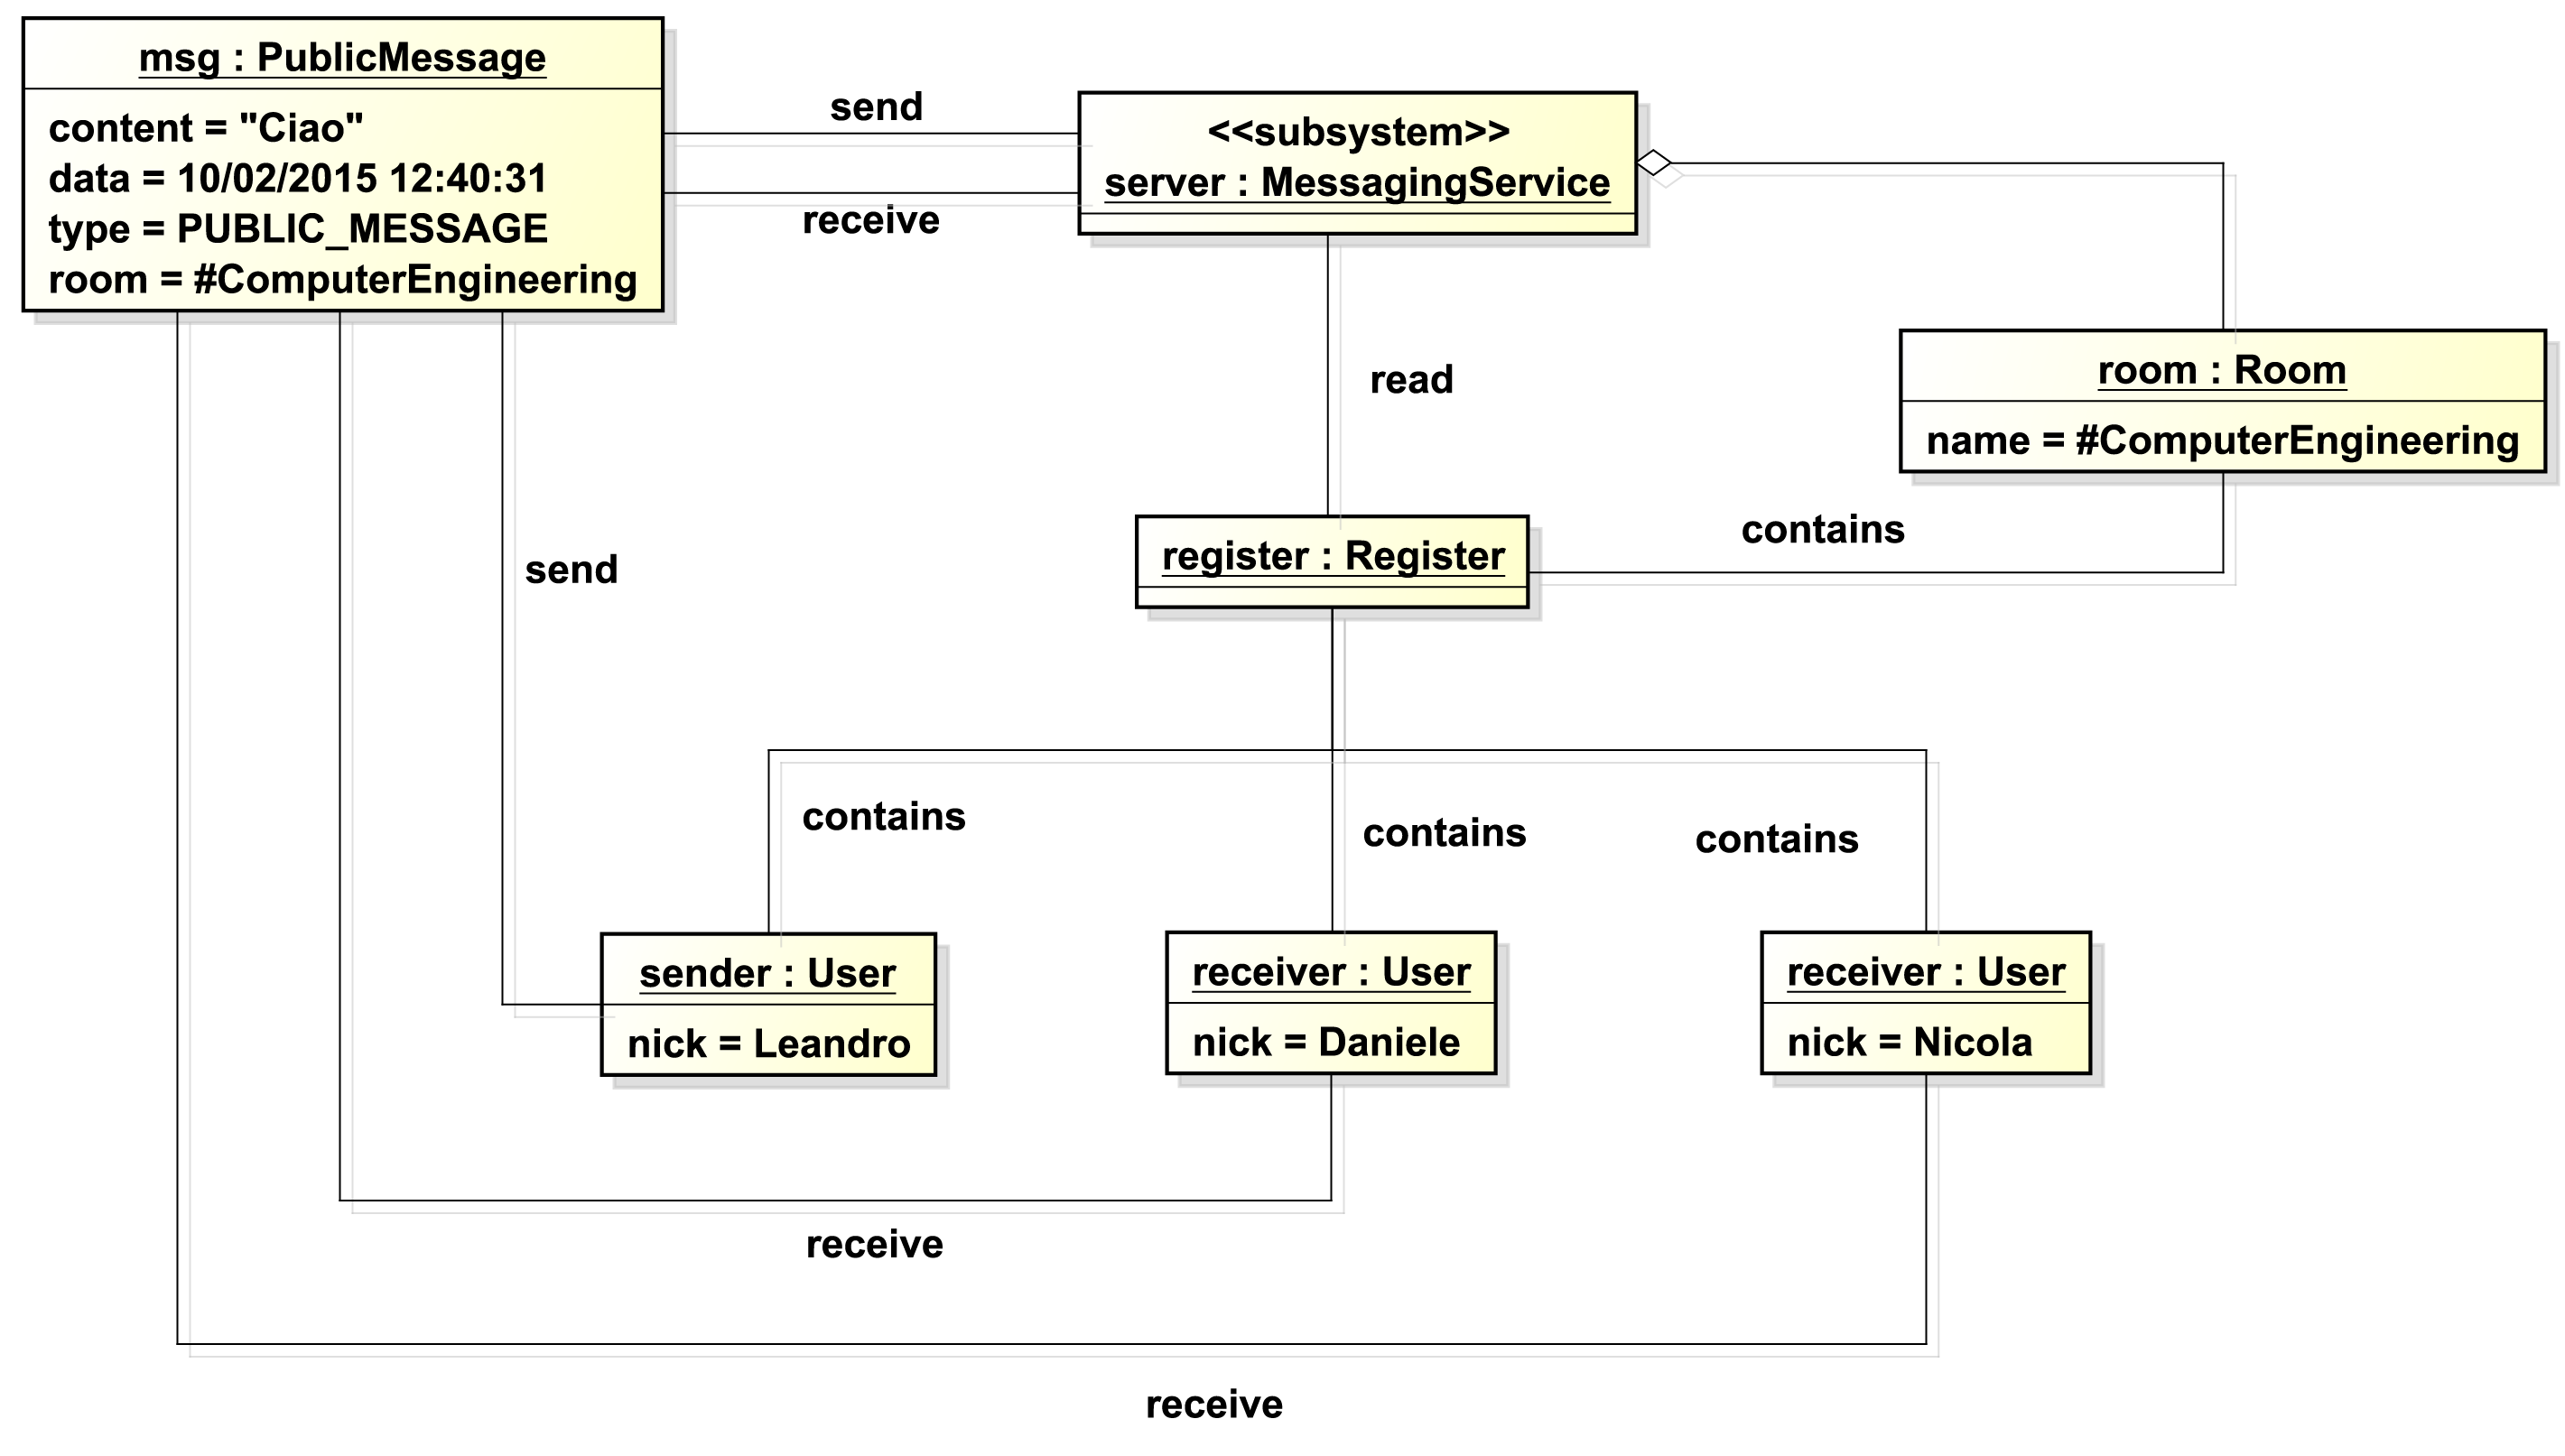
\includegraphics[scale=0.225]{image_astah/Iteration_2_DomainModel/UC3_SendPublicMessage_OM.png}{\centering}
     \caption{UC3 - Oggetti di dominio}
     \label{fig_UC3_SPM_OM} 
   \end{figure}
\end{frame}

\begin{frame} {Iterazione 2: Analisi - UC3\_SendPublicMessage}
   \begin{figure}
     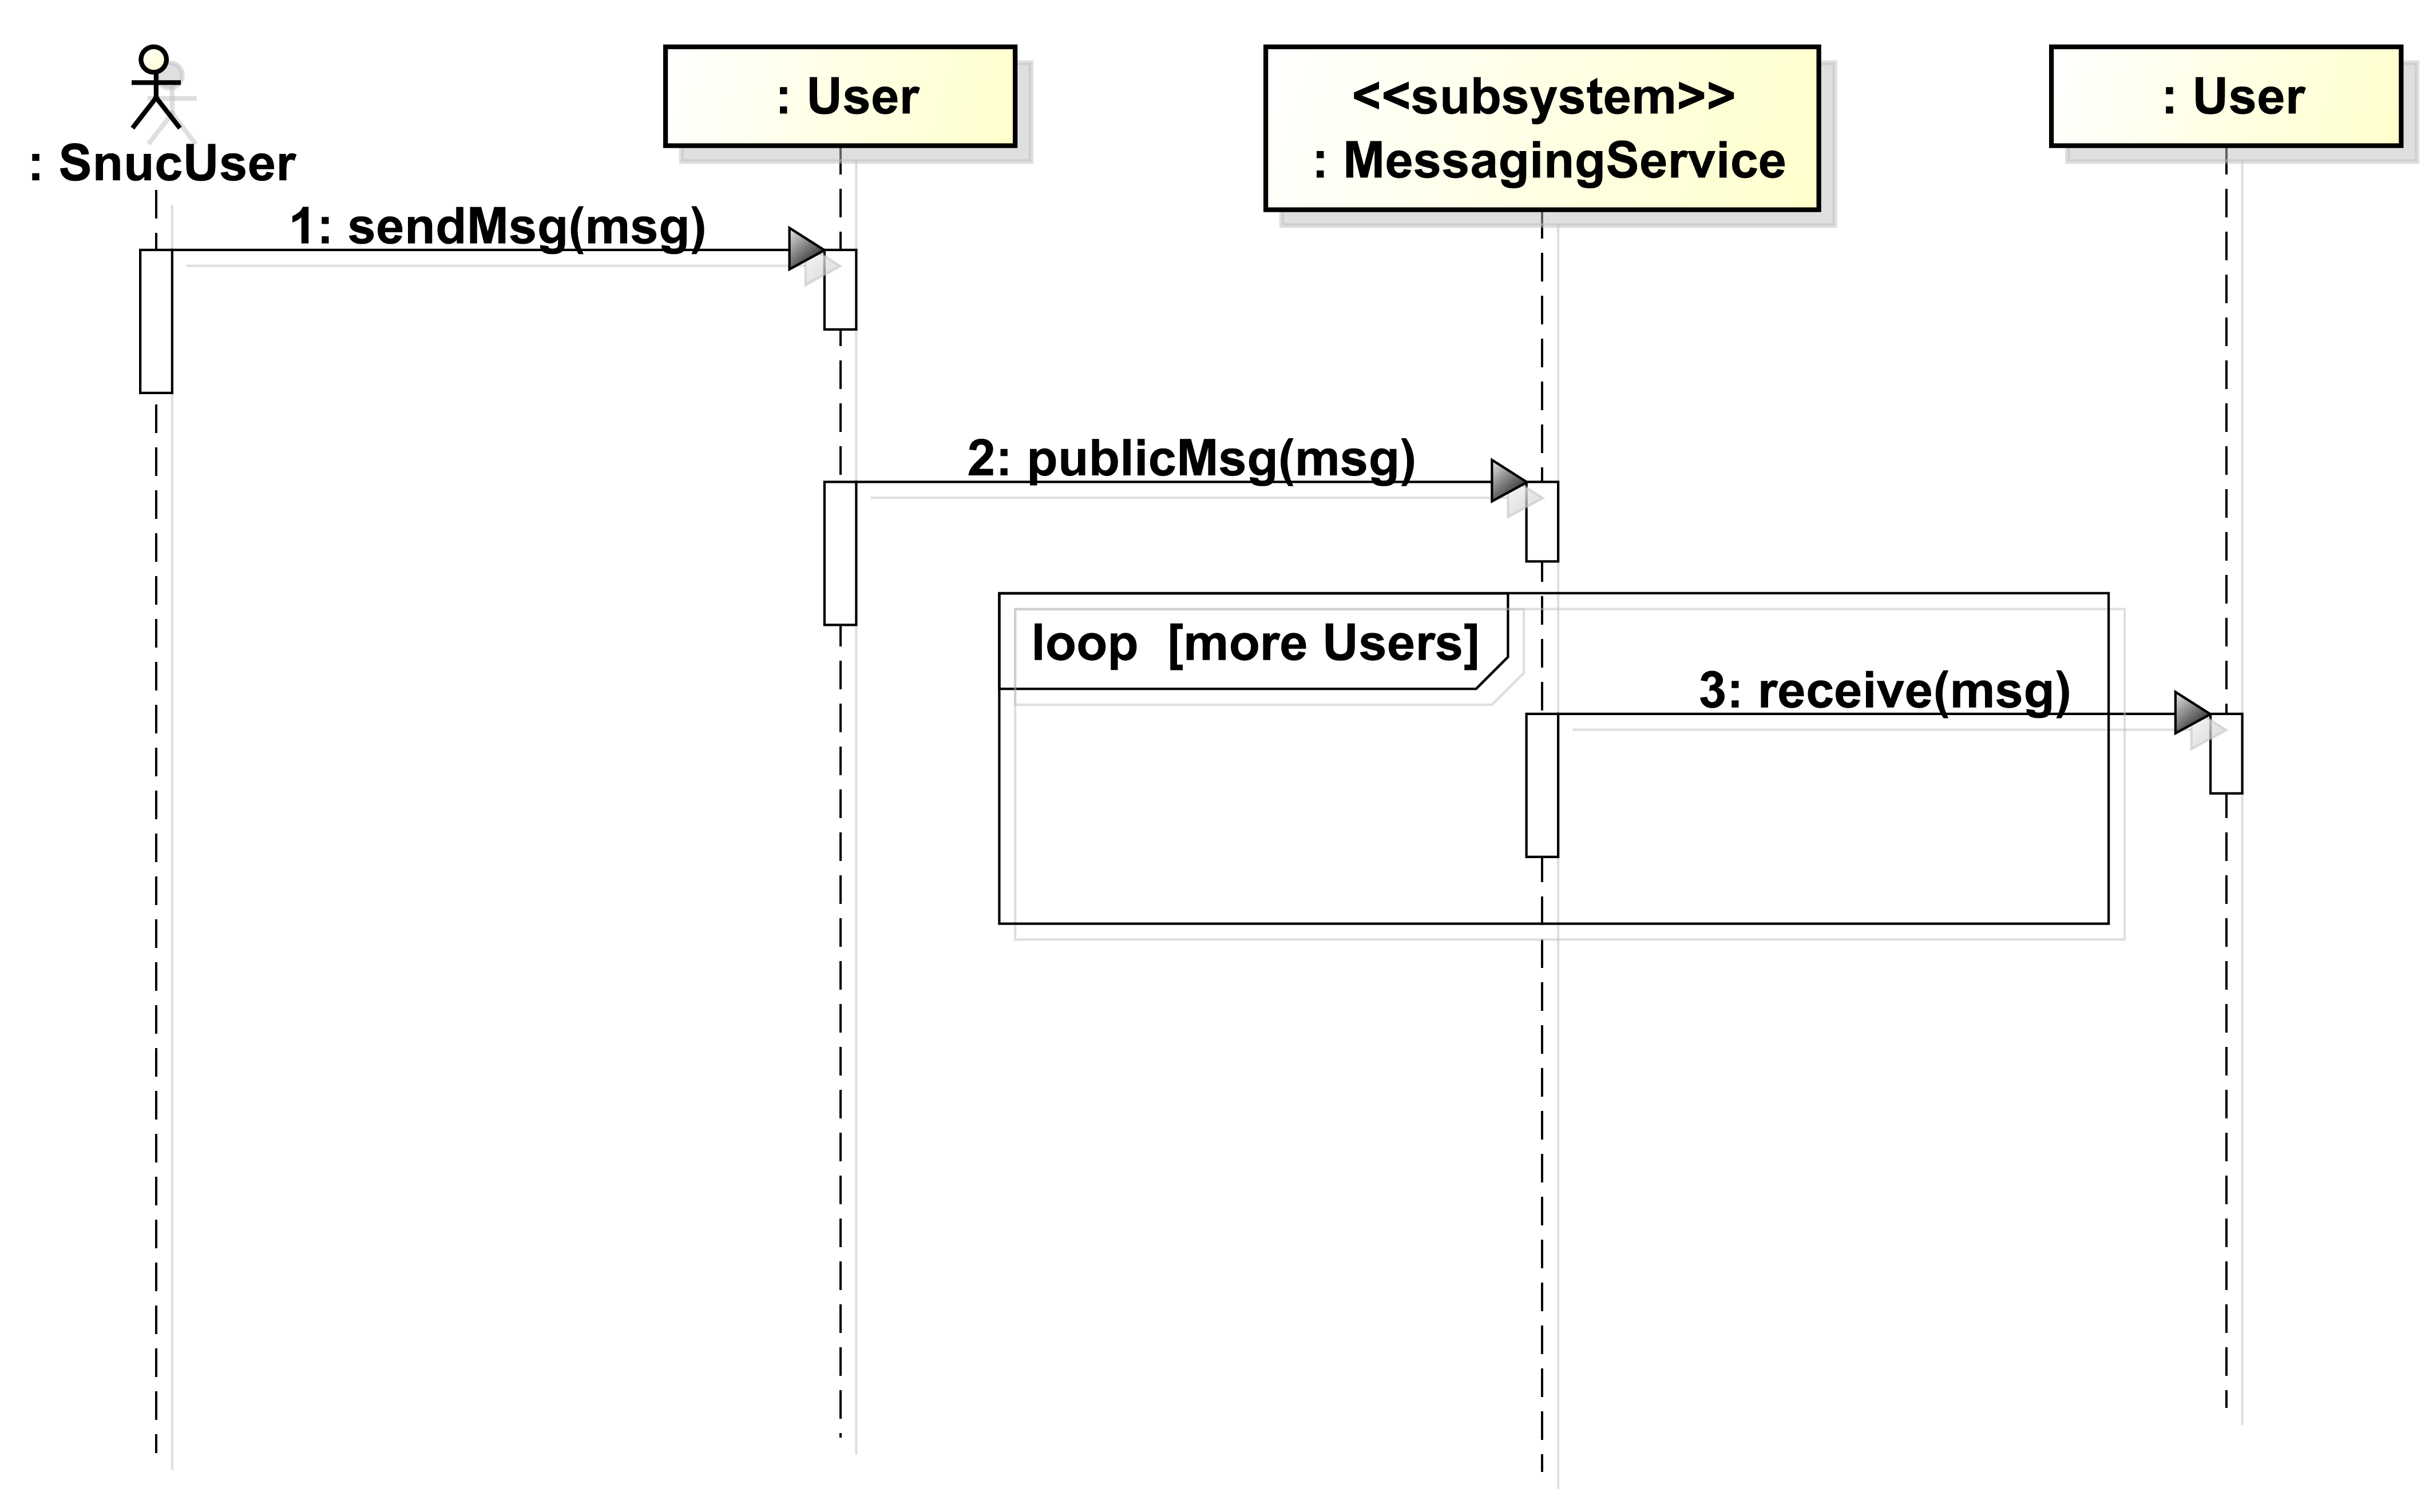
\includegraphics[scale=0.27]{image_astah/Iteration_2_DomainModel/UC3_SendPublicMessage_SSD.png}{\centering}
     \caption{UC3 - Diagramma di sequenza di sistema}
     \label{fig_UC3_SPM_SSD} 
   \end{figure}
\end{frame}

\begin{frame}
 \frametitle{Iterazione 2: Analisi, UC3 contratto CO5}
  \begin{table}[!htbp]
   \caption {UC3 Contratto CO5 - publicMsg}
    \label{table_CO5}
      \resizebox{\linewidth}{!}{%
       \begin{tabular}{|l|p{10cm}|}\hline
         Operazione & \textbf{publicMsg(msg:PublicMessage)} \\\hline 
         Riferimenti & Caso d'uso: UC3\_SendPublicMessage \\\hline
         Pre-condizione & L'utente è registrato nella stanza \\\hline 
         Post-condizione & Gli utenti registrati nella stanza ricevono il messaggio inviato \\\hline
      \end{tabular}}
   \end{table}
\end{frame}

\subsection{Iterazione 2: Progettazione}
\begin{frame} {Descrizione Iterazione 2: Progettazione}
  \emph{INSERIRE DESCRIZIONE}
\end{frame}

\subsection{Iterazione 2: Progettazione Class Diagram UC3\_SendPublicMessage}
\begin{frame} {Iterazione 2: Progettazione Class Diagram Common UC3}
   \begin{figure}
     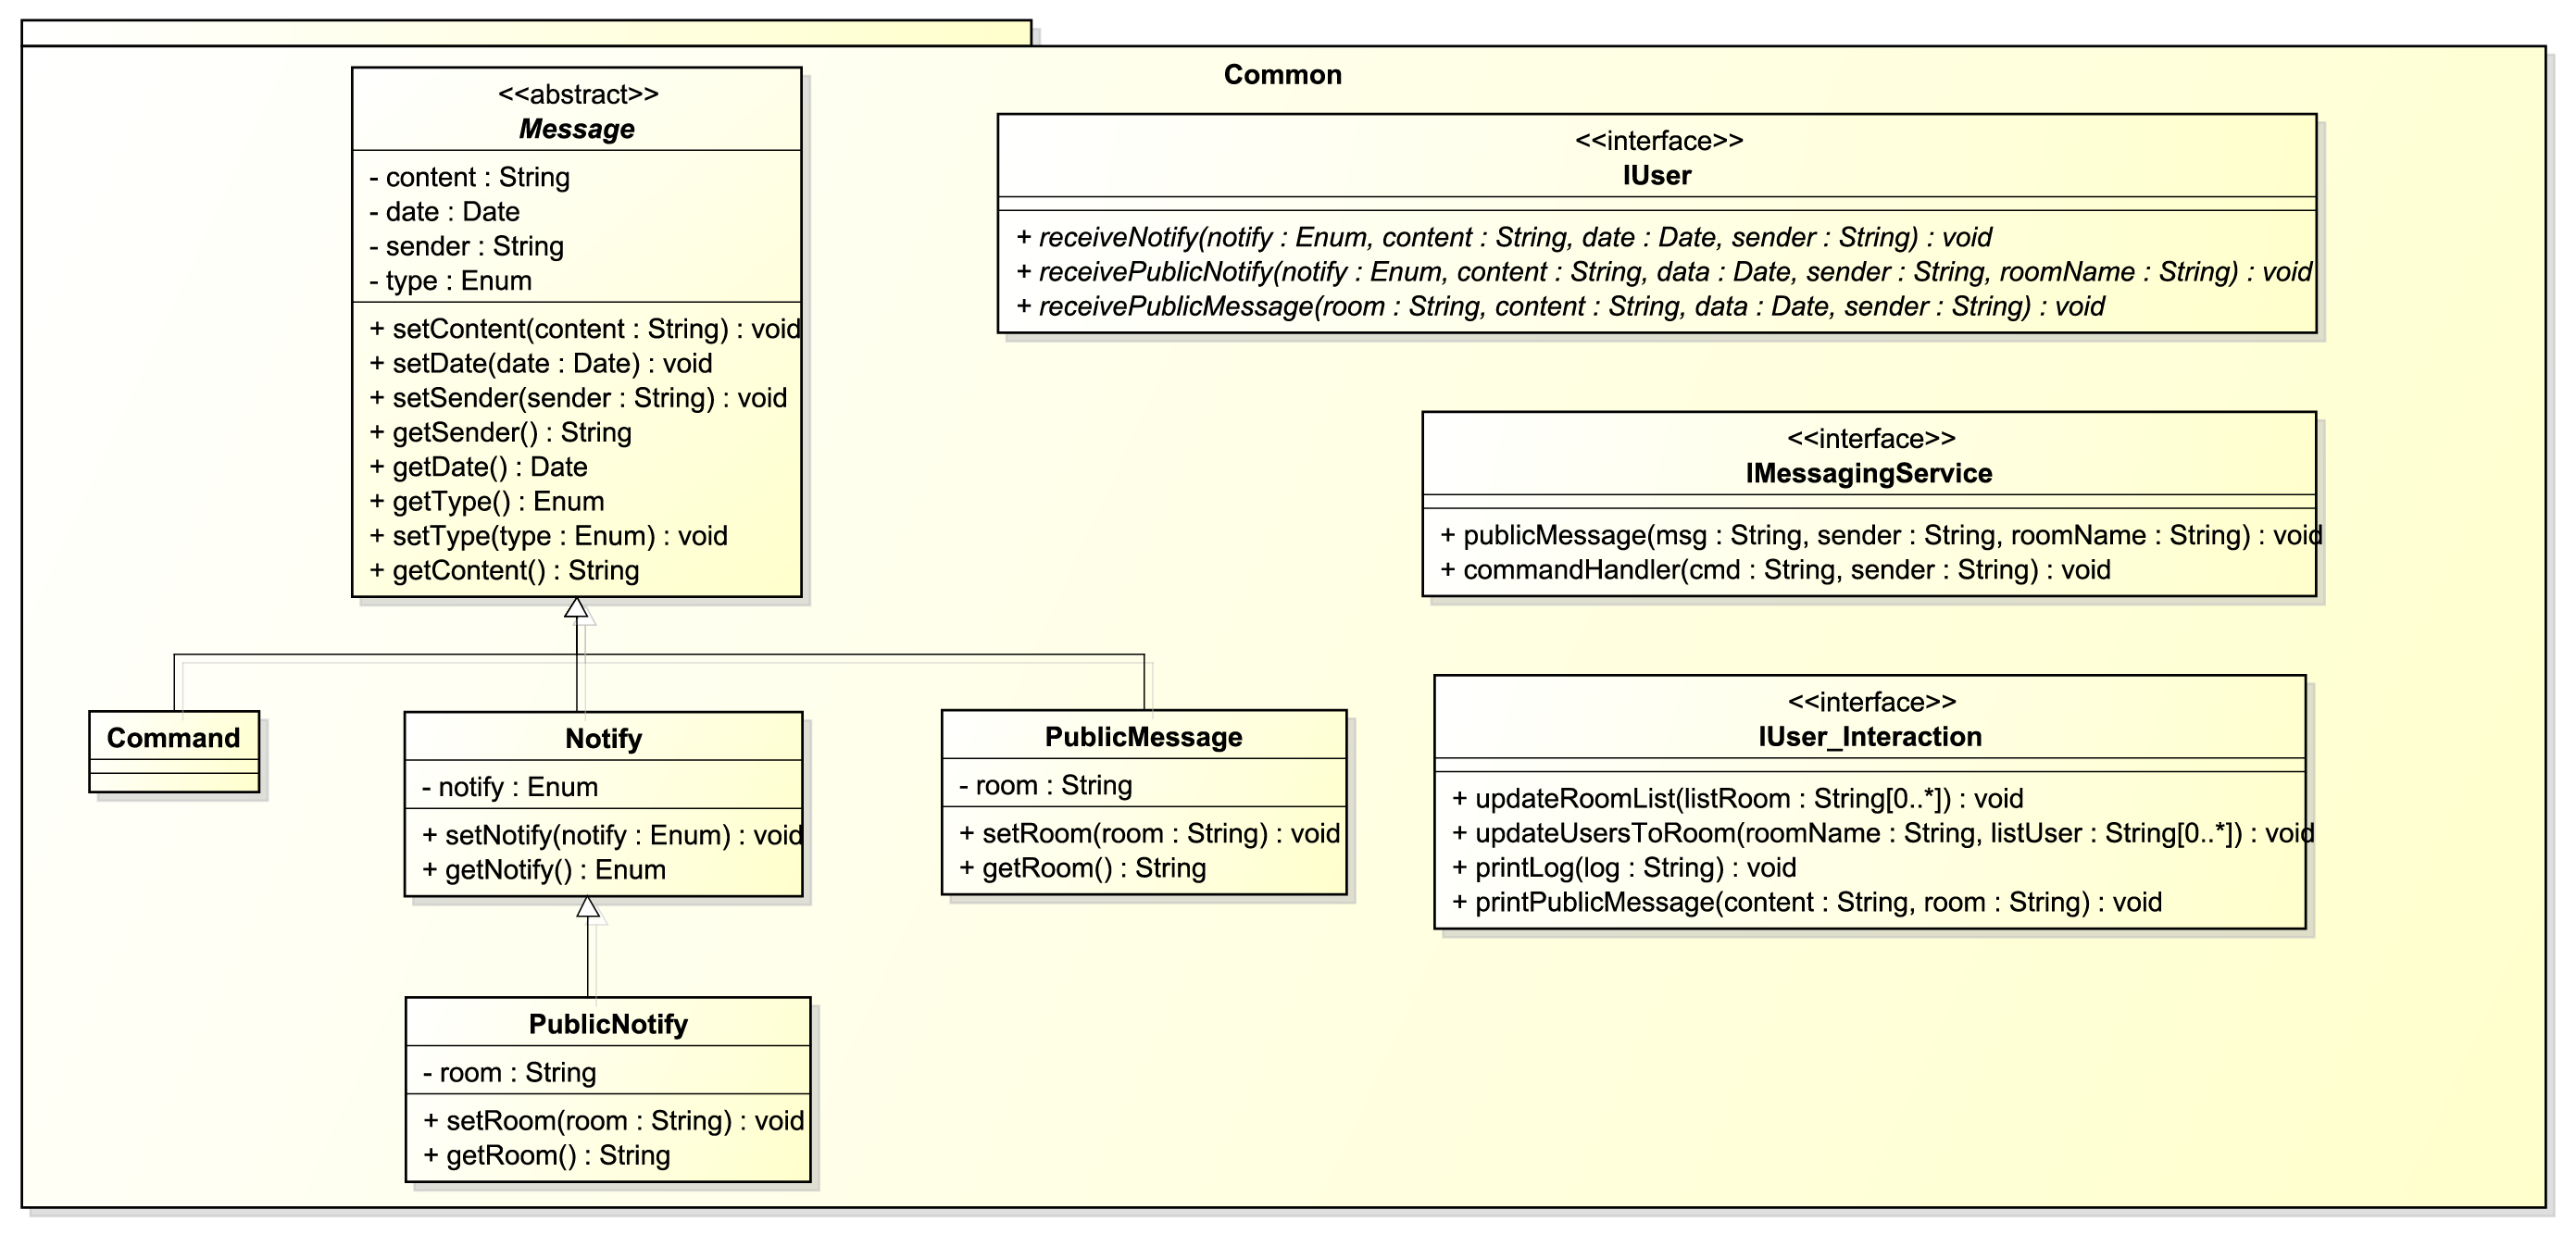
\includegraphics[scale=0.165]{image_astah/Iteration_2_DesignModel/ClassDiagramCommon.png}{\centering}
     \caption{DCD - Diagramma delle Classi: Package Common }
     \label{fig_UC3_DCD_1} 
   \end{figure}
\end{frame}

\begin{frame} {Iterazione 2: Progettazione - Class Diagram Snuc UC3}
   \begin{figure}
     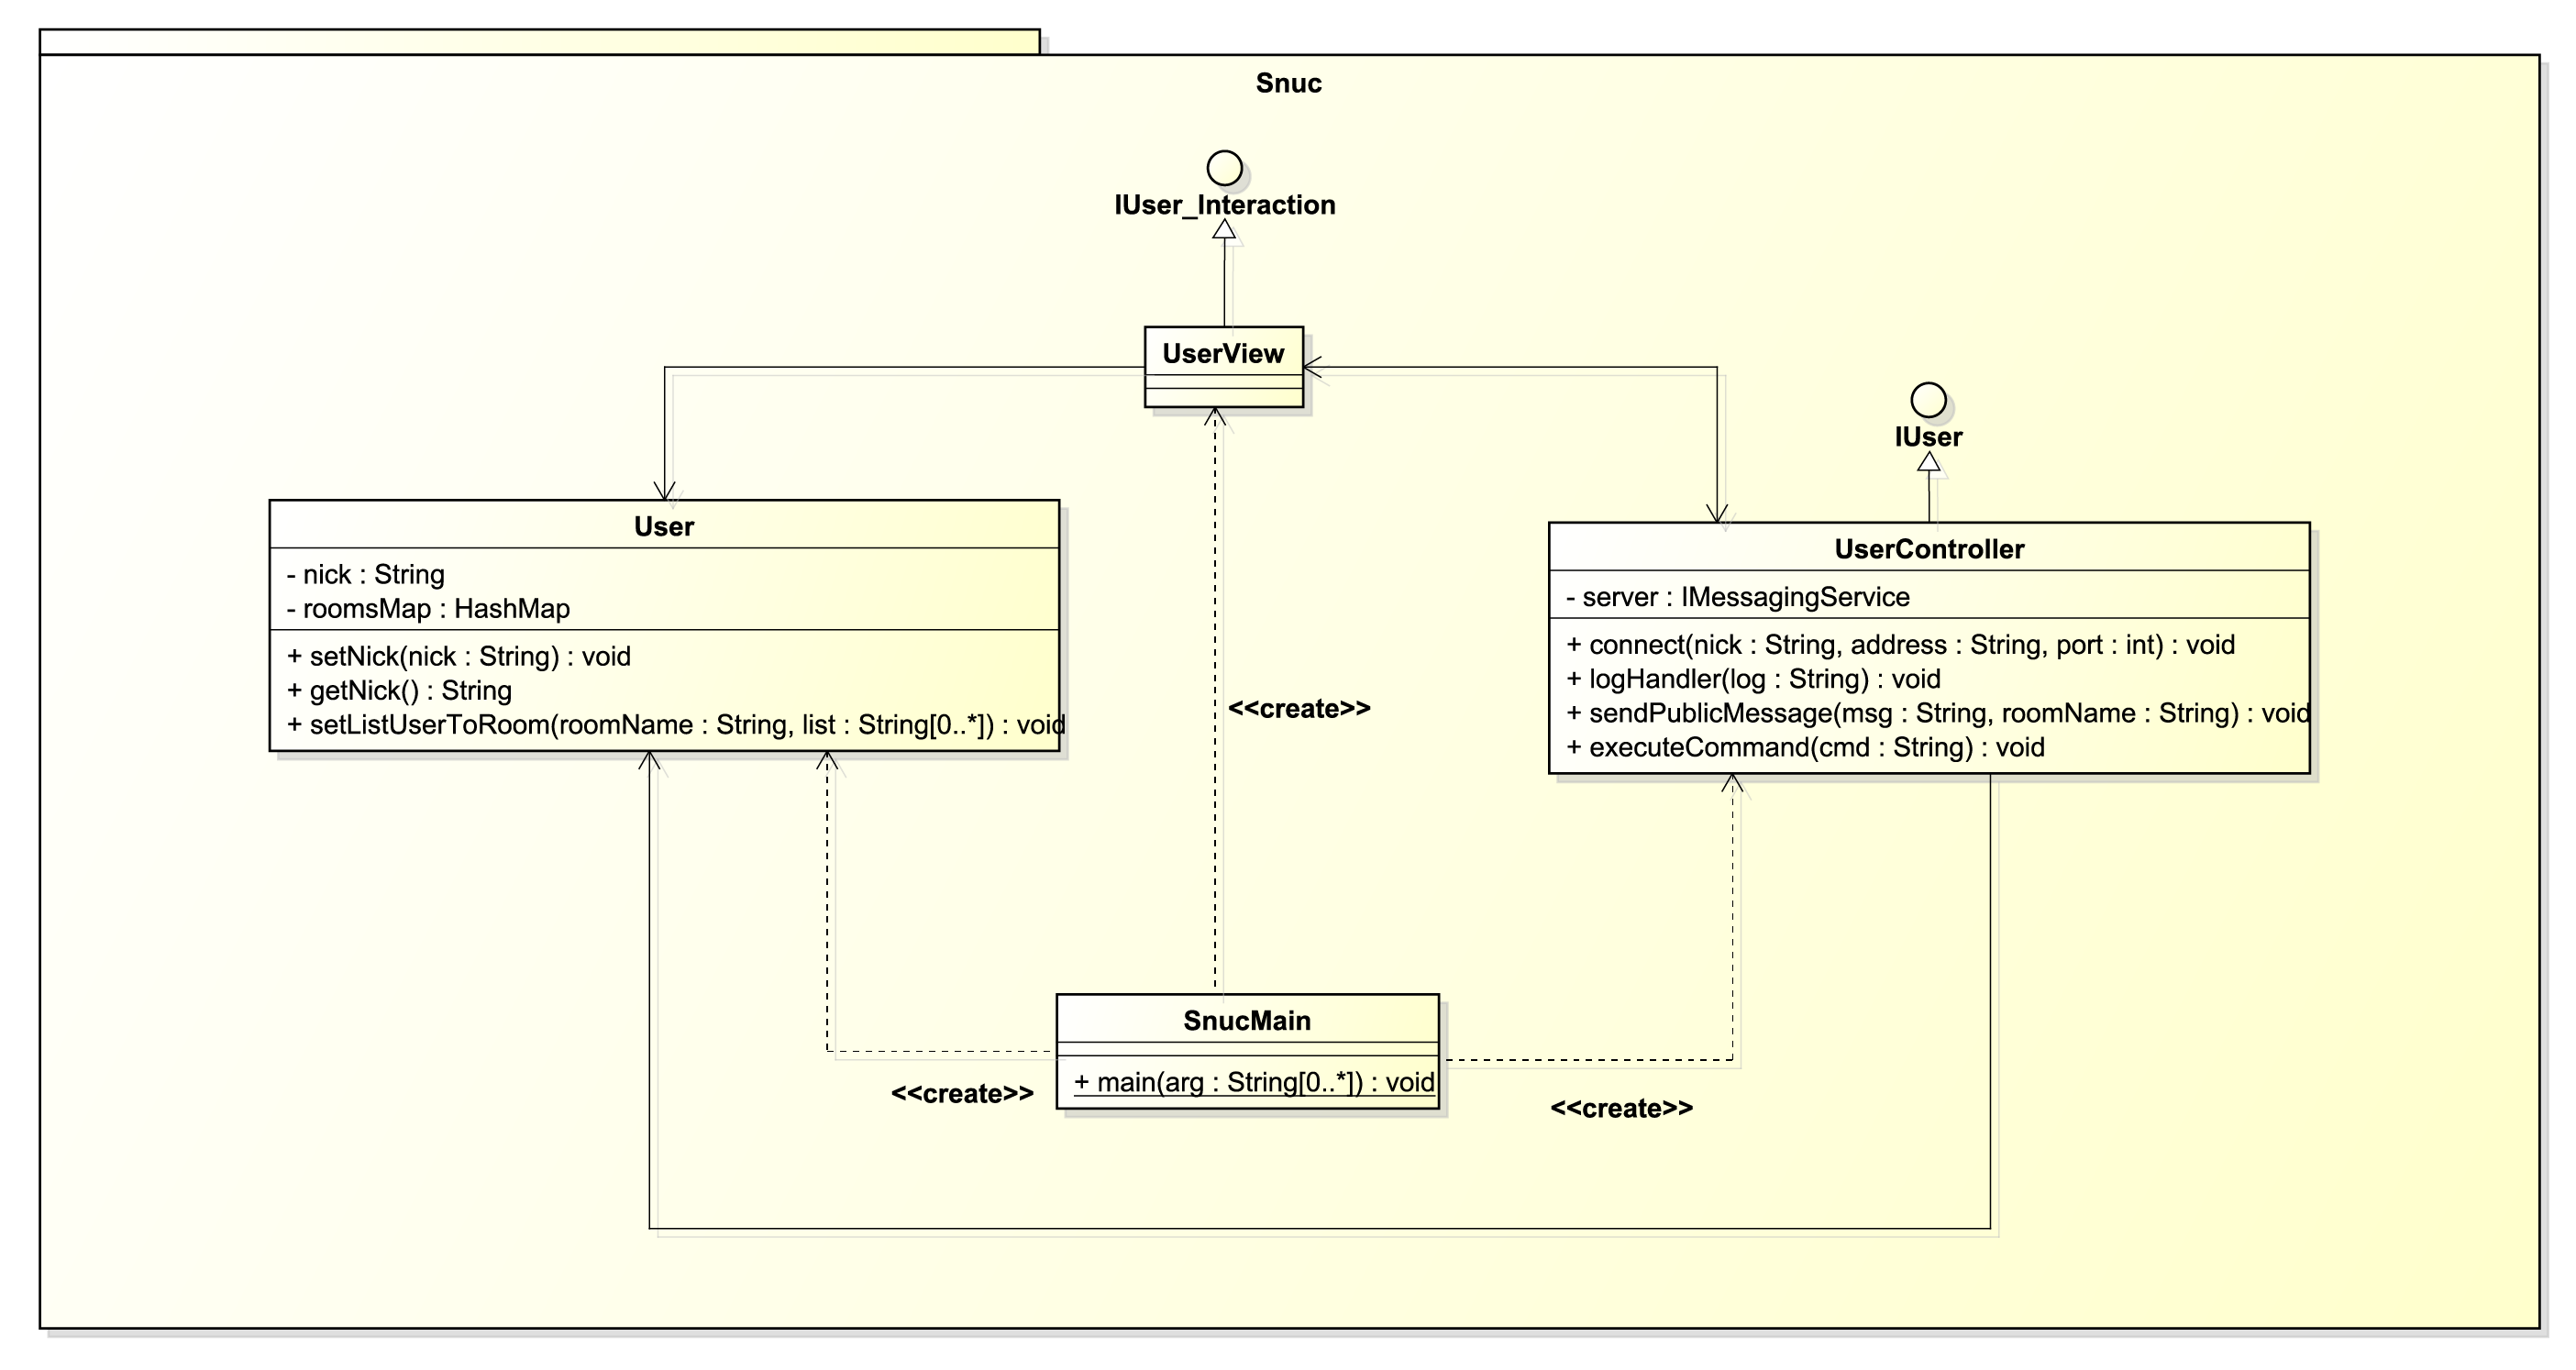
\includegraphics[scale=0.16]{image_astah/Iteration_2_DesignModel/ClassDiagramSnuc.png}{\centering}
     \caption{DCD - Diagramma delle Classi: Package Snuc }
     \label{fig_UC3_DCD_3} 
   \end{figure}
\end{frame}

\begin{frame} {Iterazione 2: Progettazione - Class Diagram Connector UC3}
   \begin{figure}
     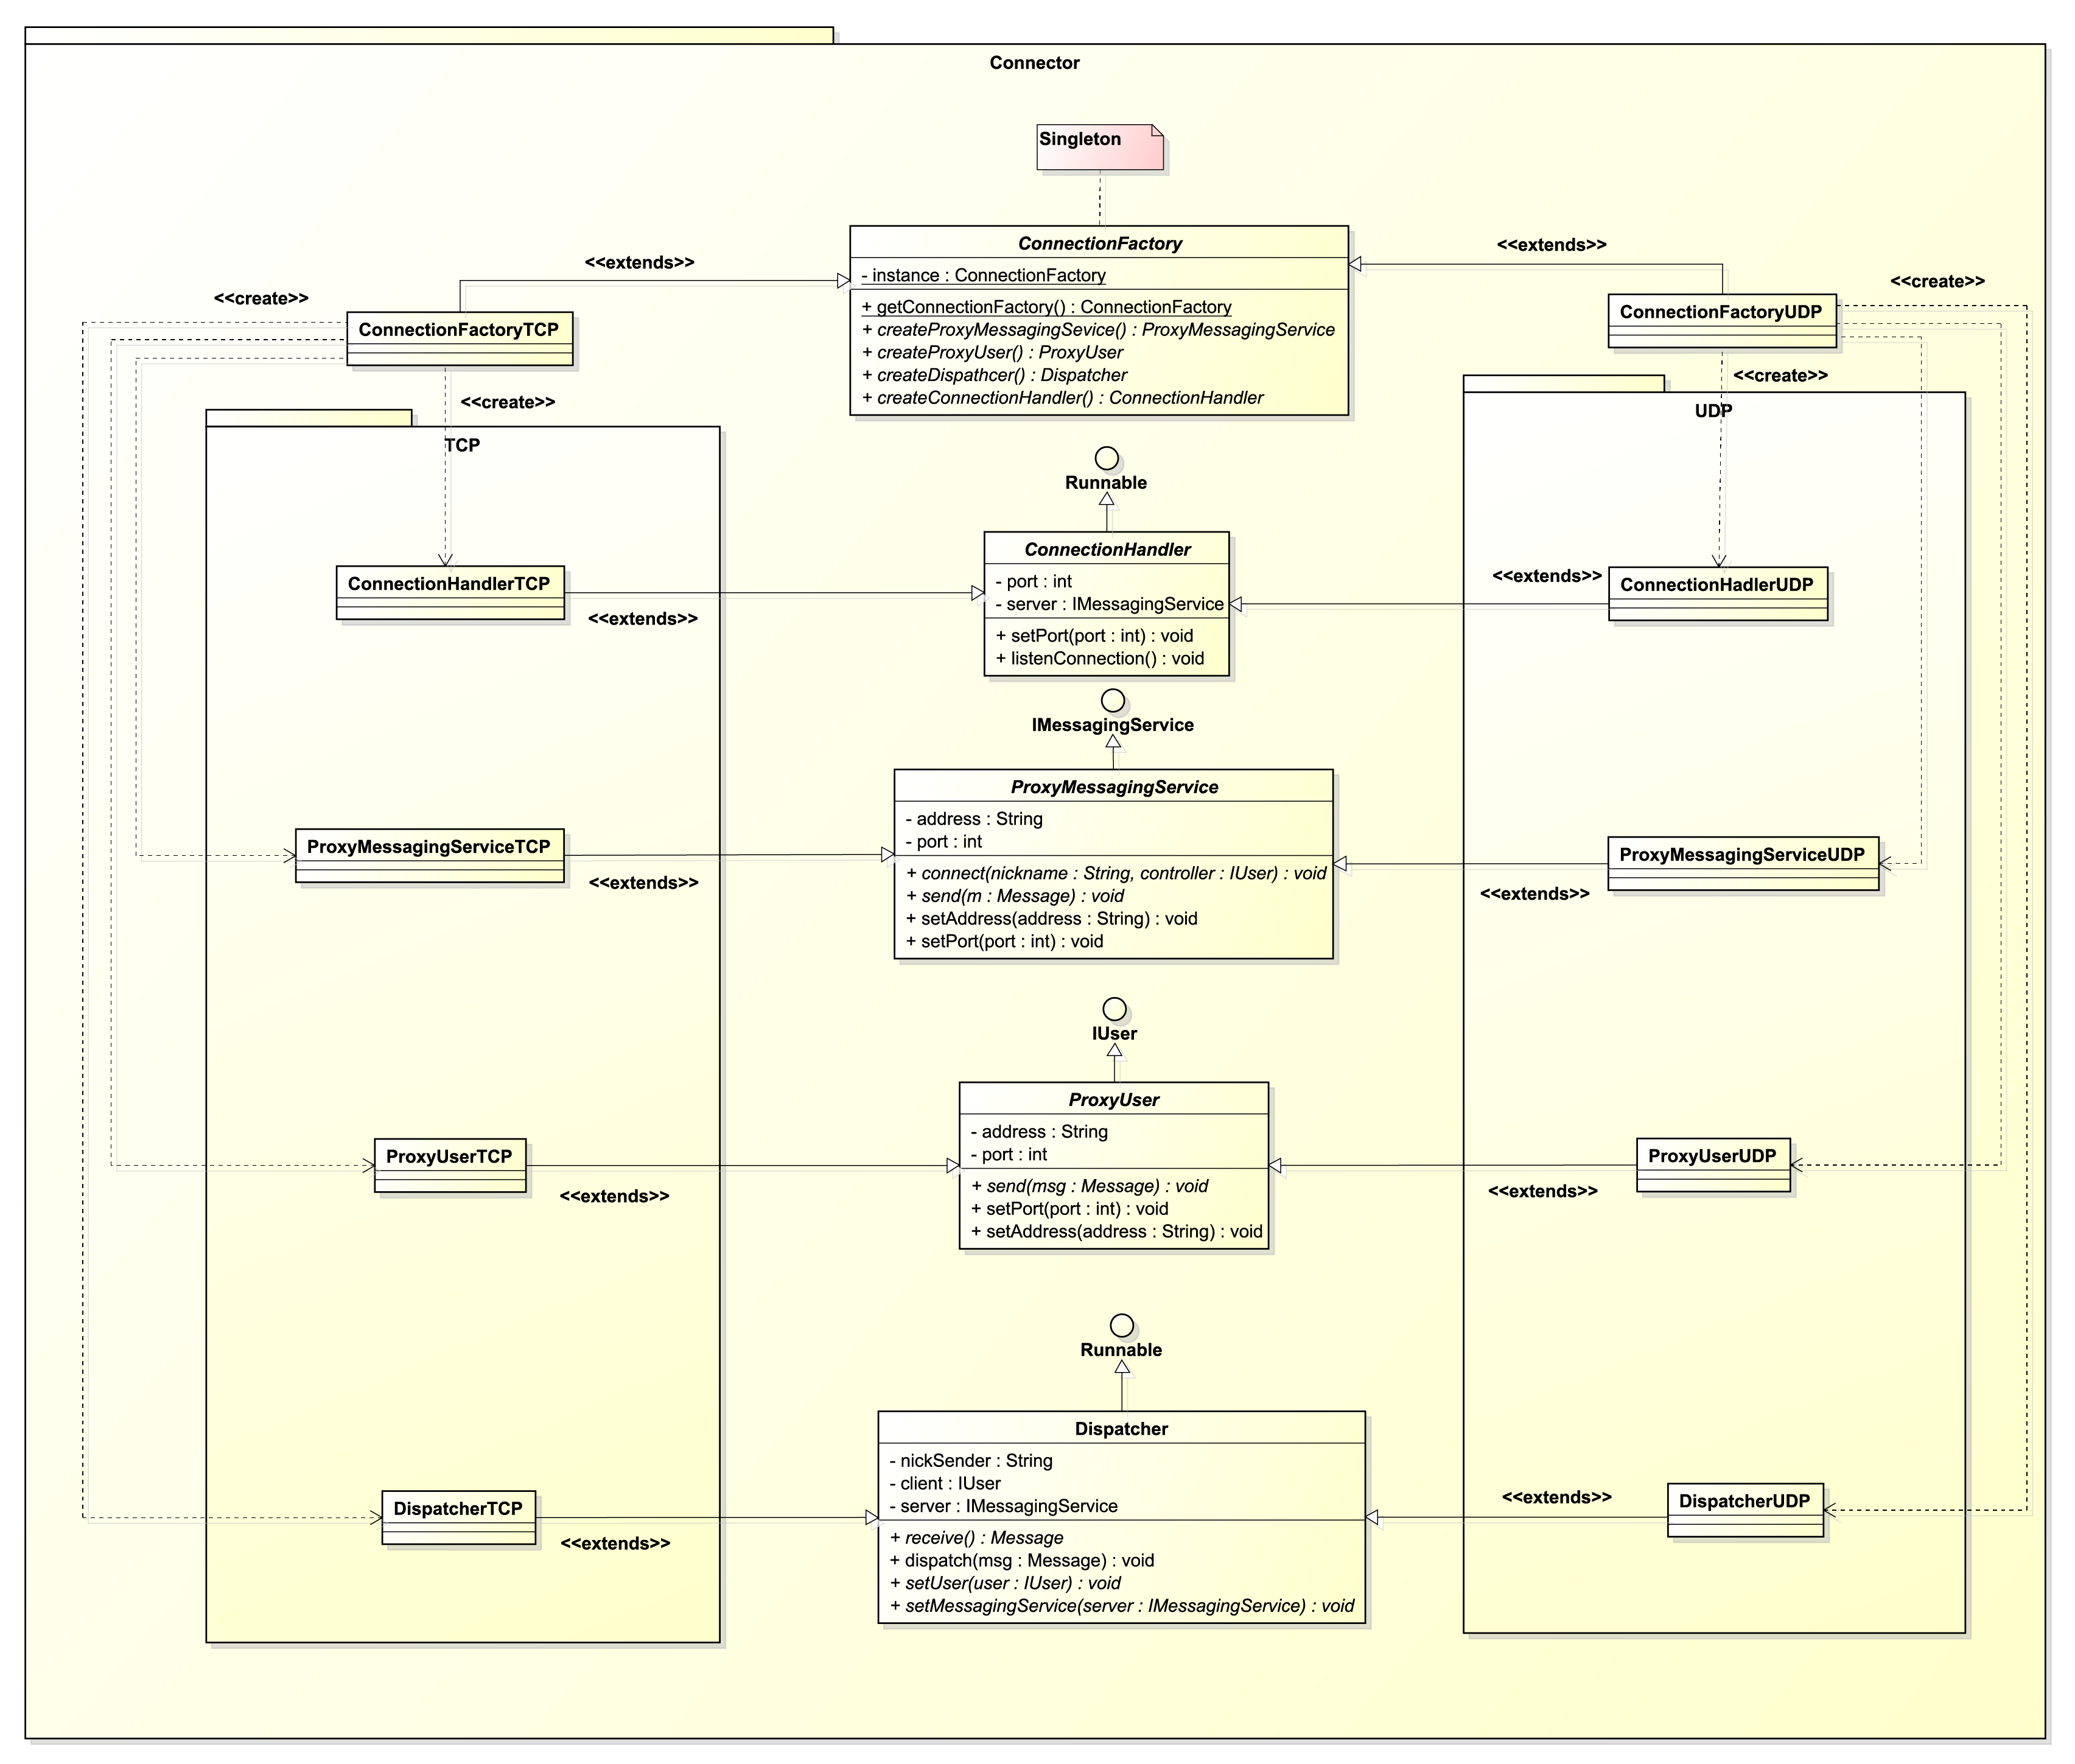
\includegraphics[scale=0.081]{image_astah/Iteration_2_DesignModel/ClassDiagramConnector.png}{\centering}
     \caption{DCD - Diagramma delle Classi: Package Connector }
     \label{fig_UC3_DCD_4} 
   \end{figure}
\end{frame}

\begin{frame} {Iterazione 2: Progettazione - Class Diagram Snuc Server UC3}
   \begin{figure}
     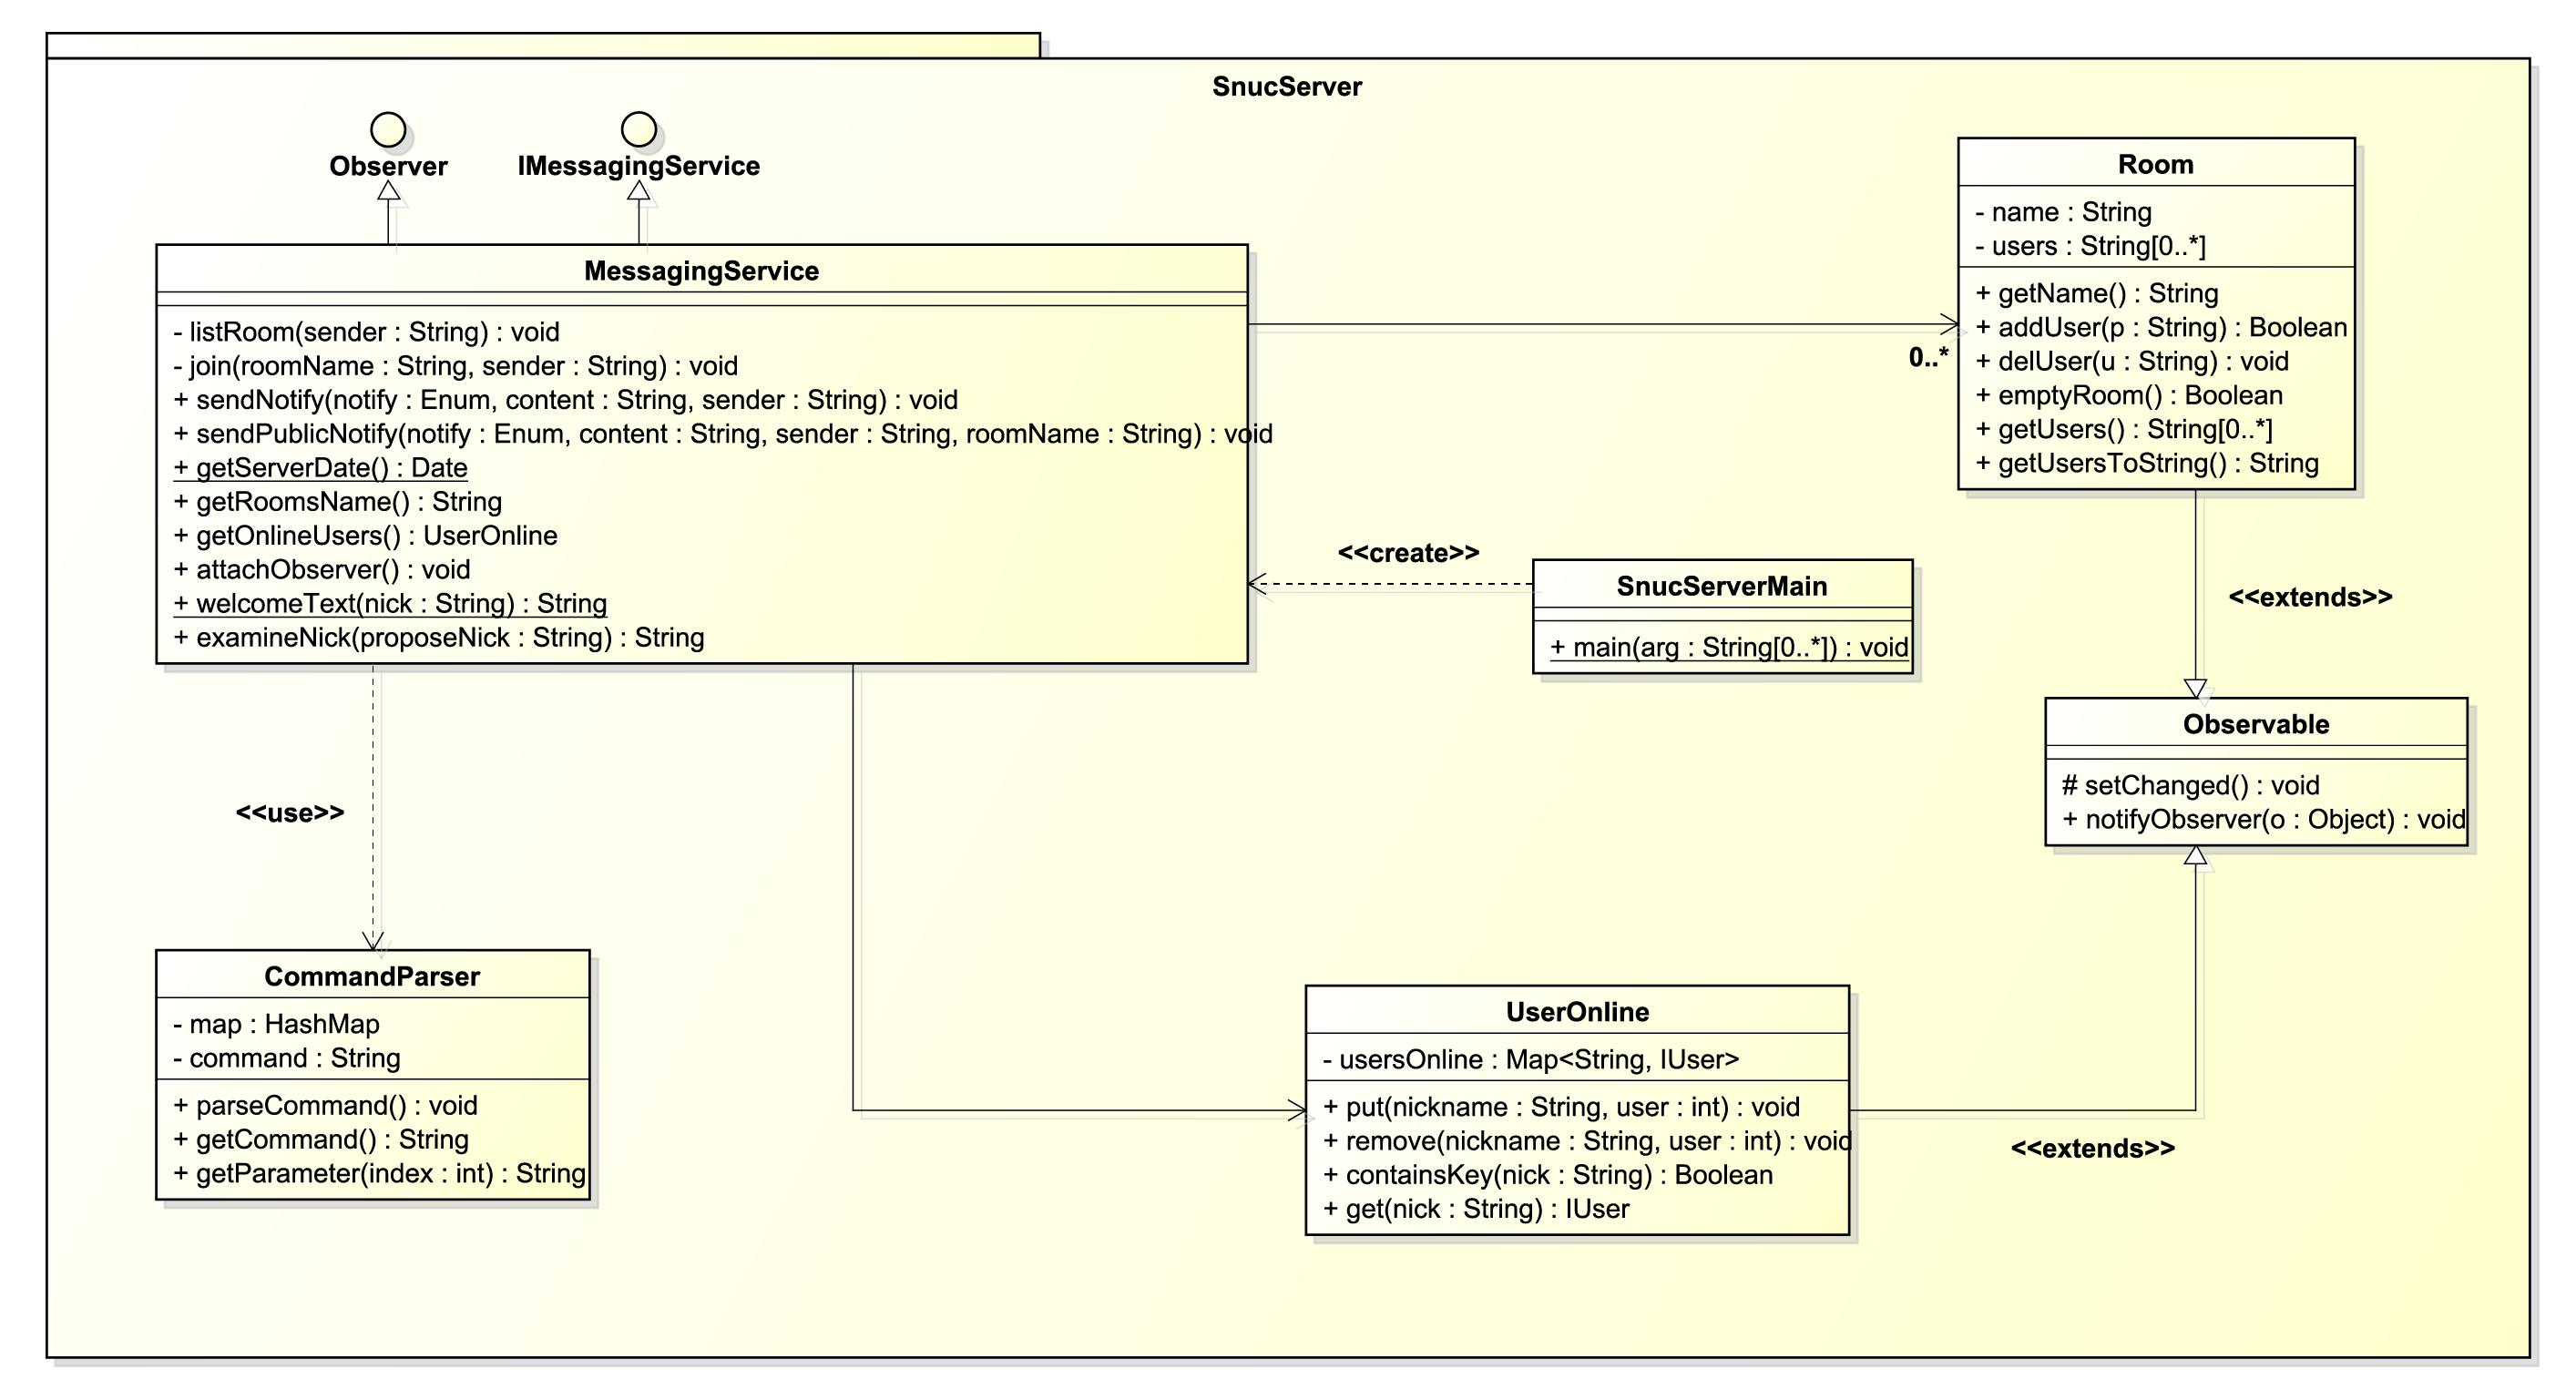
\includegraphics[scale=0.155]{image_astah/Iteration_2_DesignModel/ClassDiagramSnucServer.png}{\centering}
     \caption{DCD - Diagramma delle Classi: Package Snuc Server }
     \label{fig_UC3_DCD_2} 
   \end{figure}
\end{frame}

\subsection{Iterazione 2: Progettazione - SSD UC3\_SendPublicMessage}
\begin{frame} {Iterazione 2: Progettazione, UC3\_SendPublicMessage - OP1}
   \begin{figure}
     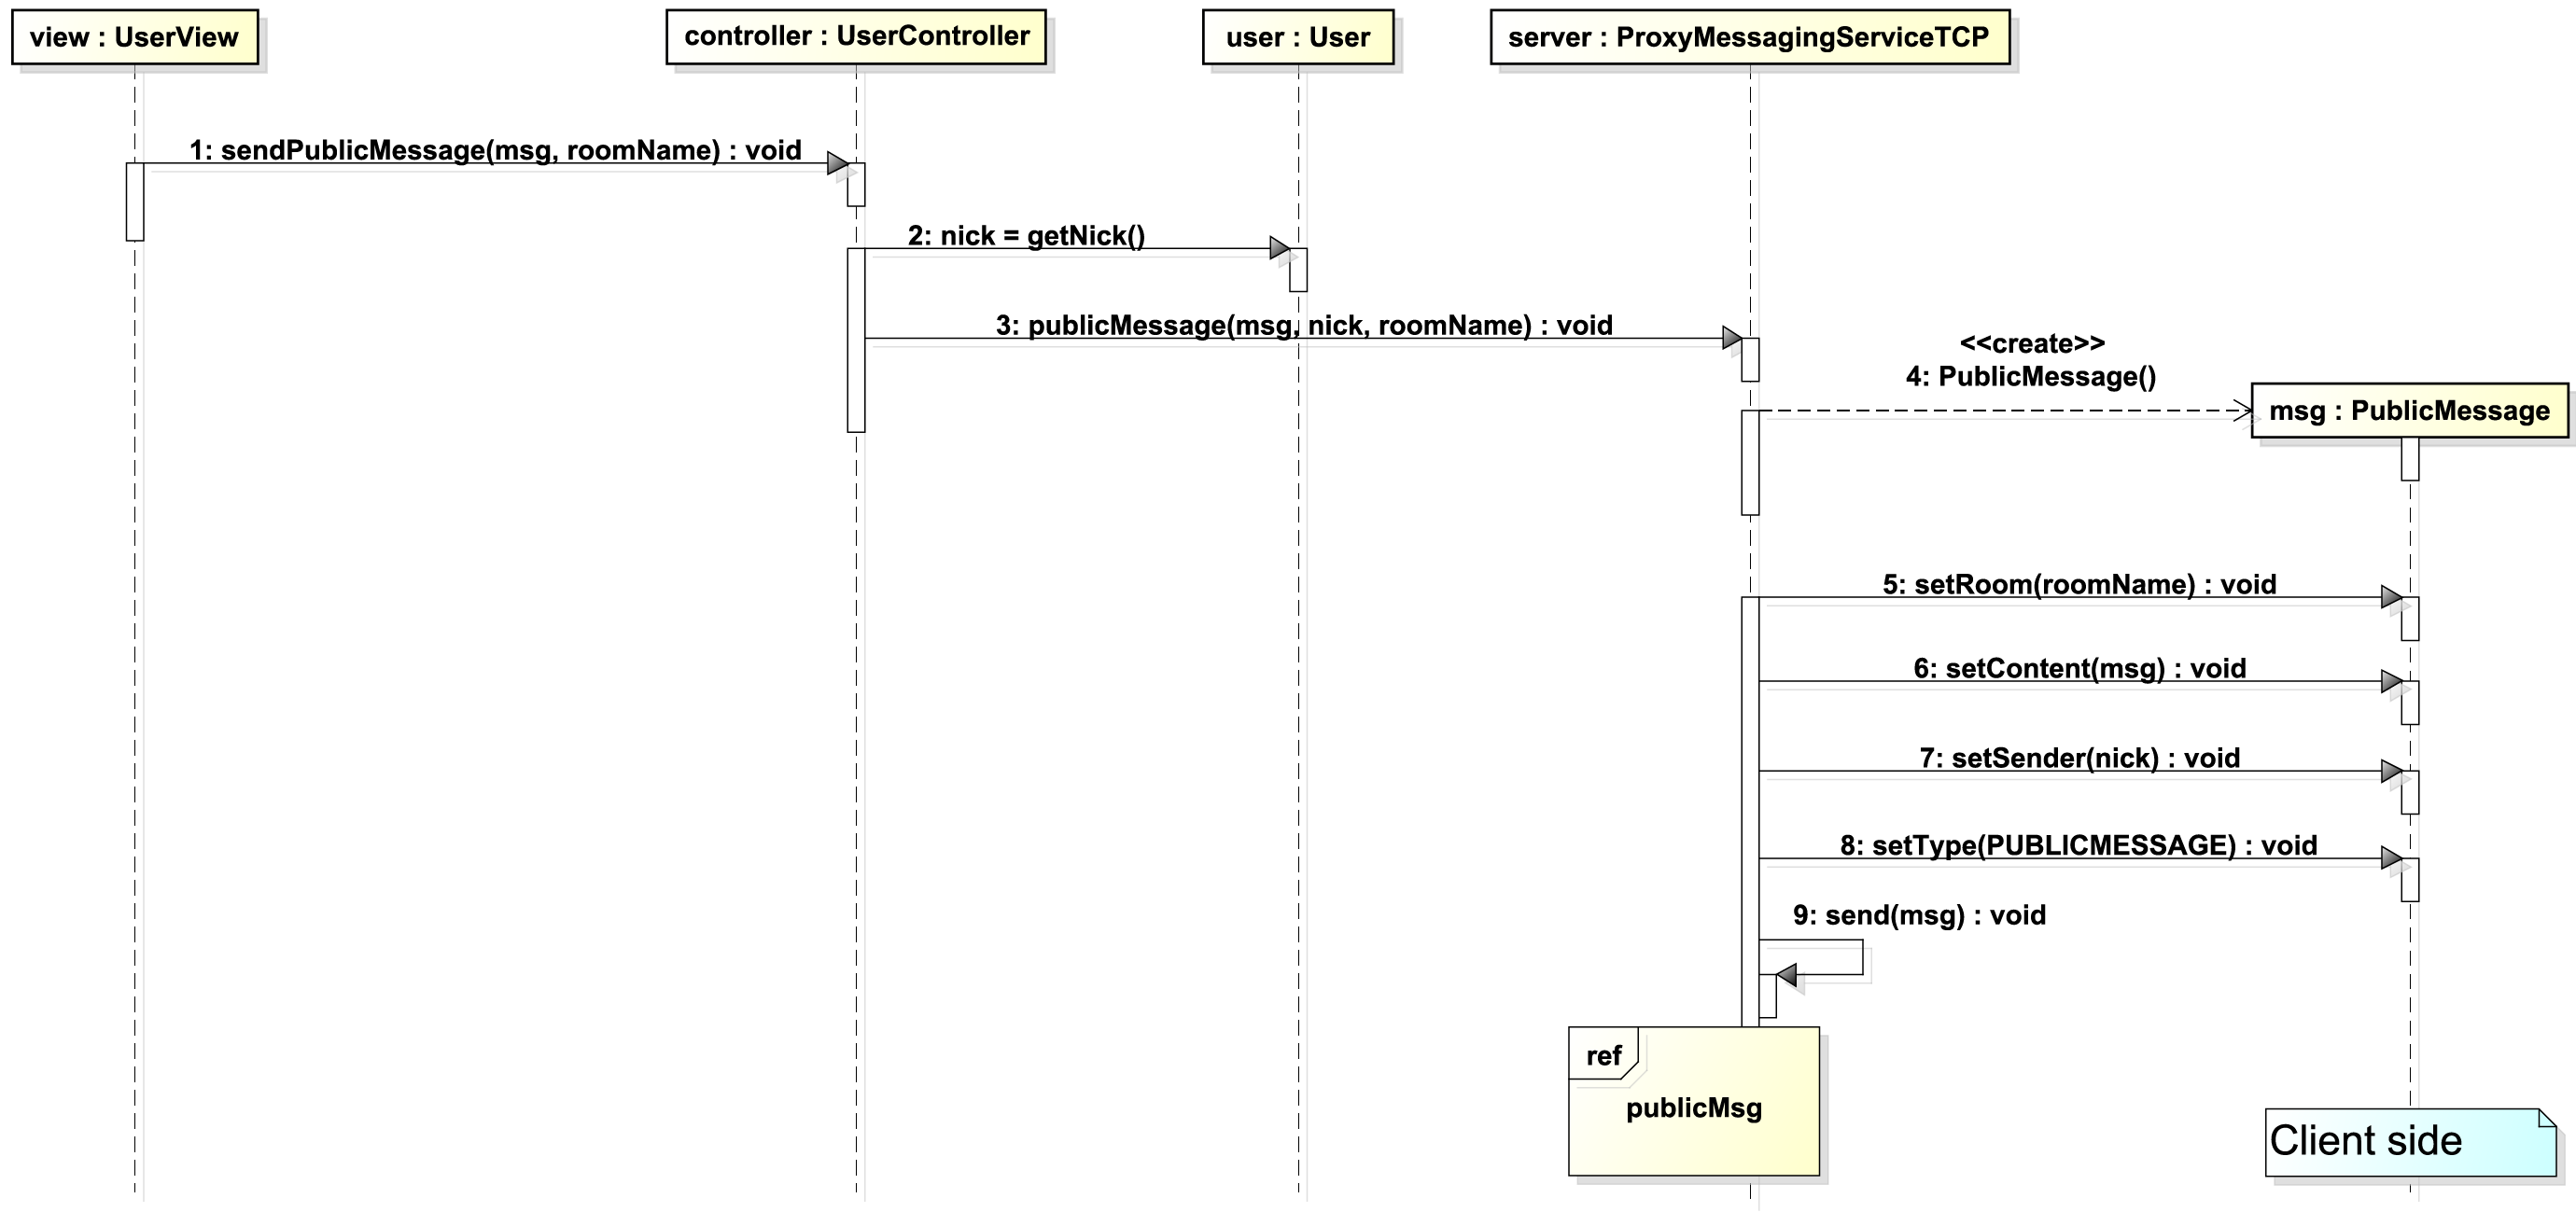
\includegraphics[scale=0.16]{image_astah/Iteration_2_DesignModel/UC3_SendPublicMessage_SSD_1_sendMsg.png}{\centering}
     \caption{SSD - OP1: sendMsg(msg) del modello di dominio (figura \ref{fig_UC3_SPM_SSD}) }
     \label{fig_UC3_SSD_SRM_1} 
   \end{figure}
\end{frame}

\begin{frame} {Iterazione 2: Progettazione, UC3\_SendPublicMessage - OP2}
   \begin{figure}
     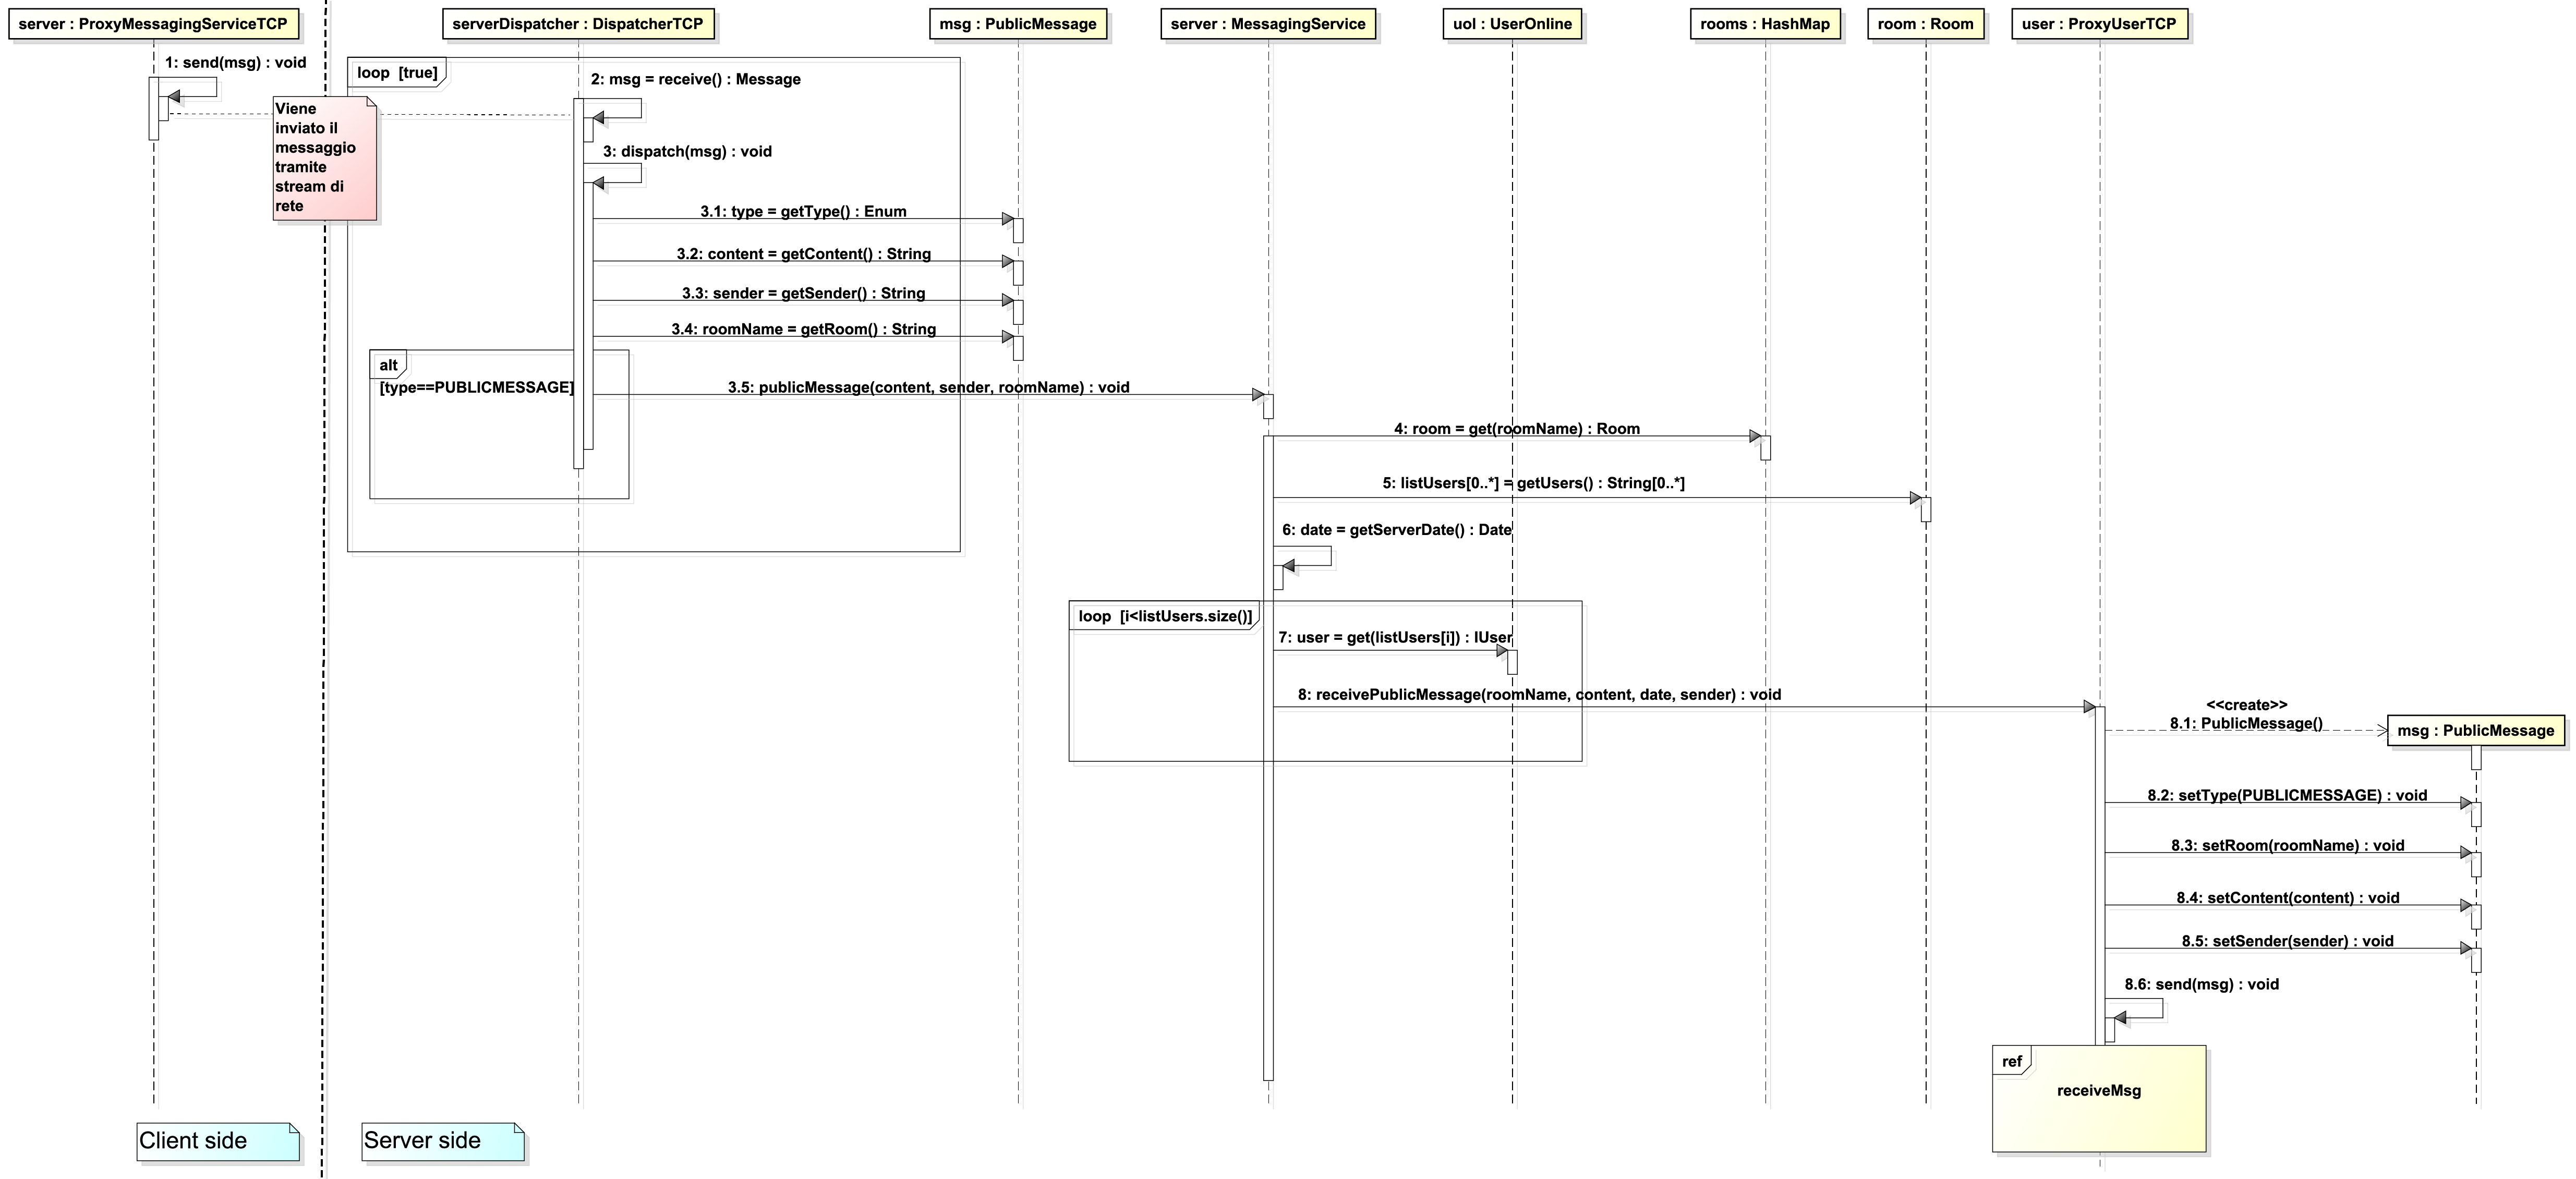
\includegraphics[scale=0.09]{image_astah/Iteration_2_DesignModel/UC3_SendPublicMessage_SSD_2_publicMsg.png}{\centering}
     \caption{SSD - OP2: pubblicMsg(msg) del modello di dominio (figura \ref{fig_UC3_SPM_SSD}) }
     \label{fig_UC3_SSD_SRM_2} 
   \end{figure}
\end{frame}

\begin{frame} {Iterazione 2: Progettazione, UC3\_SendPublicMessage - OP3}
   \begin{figure}
     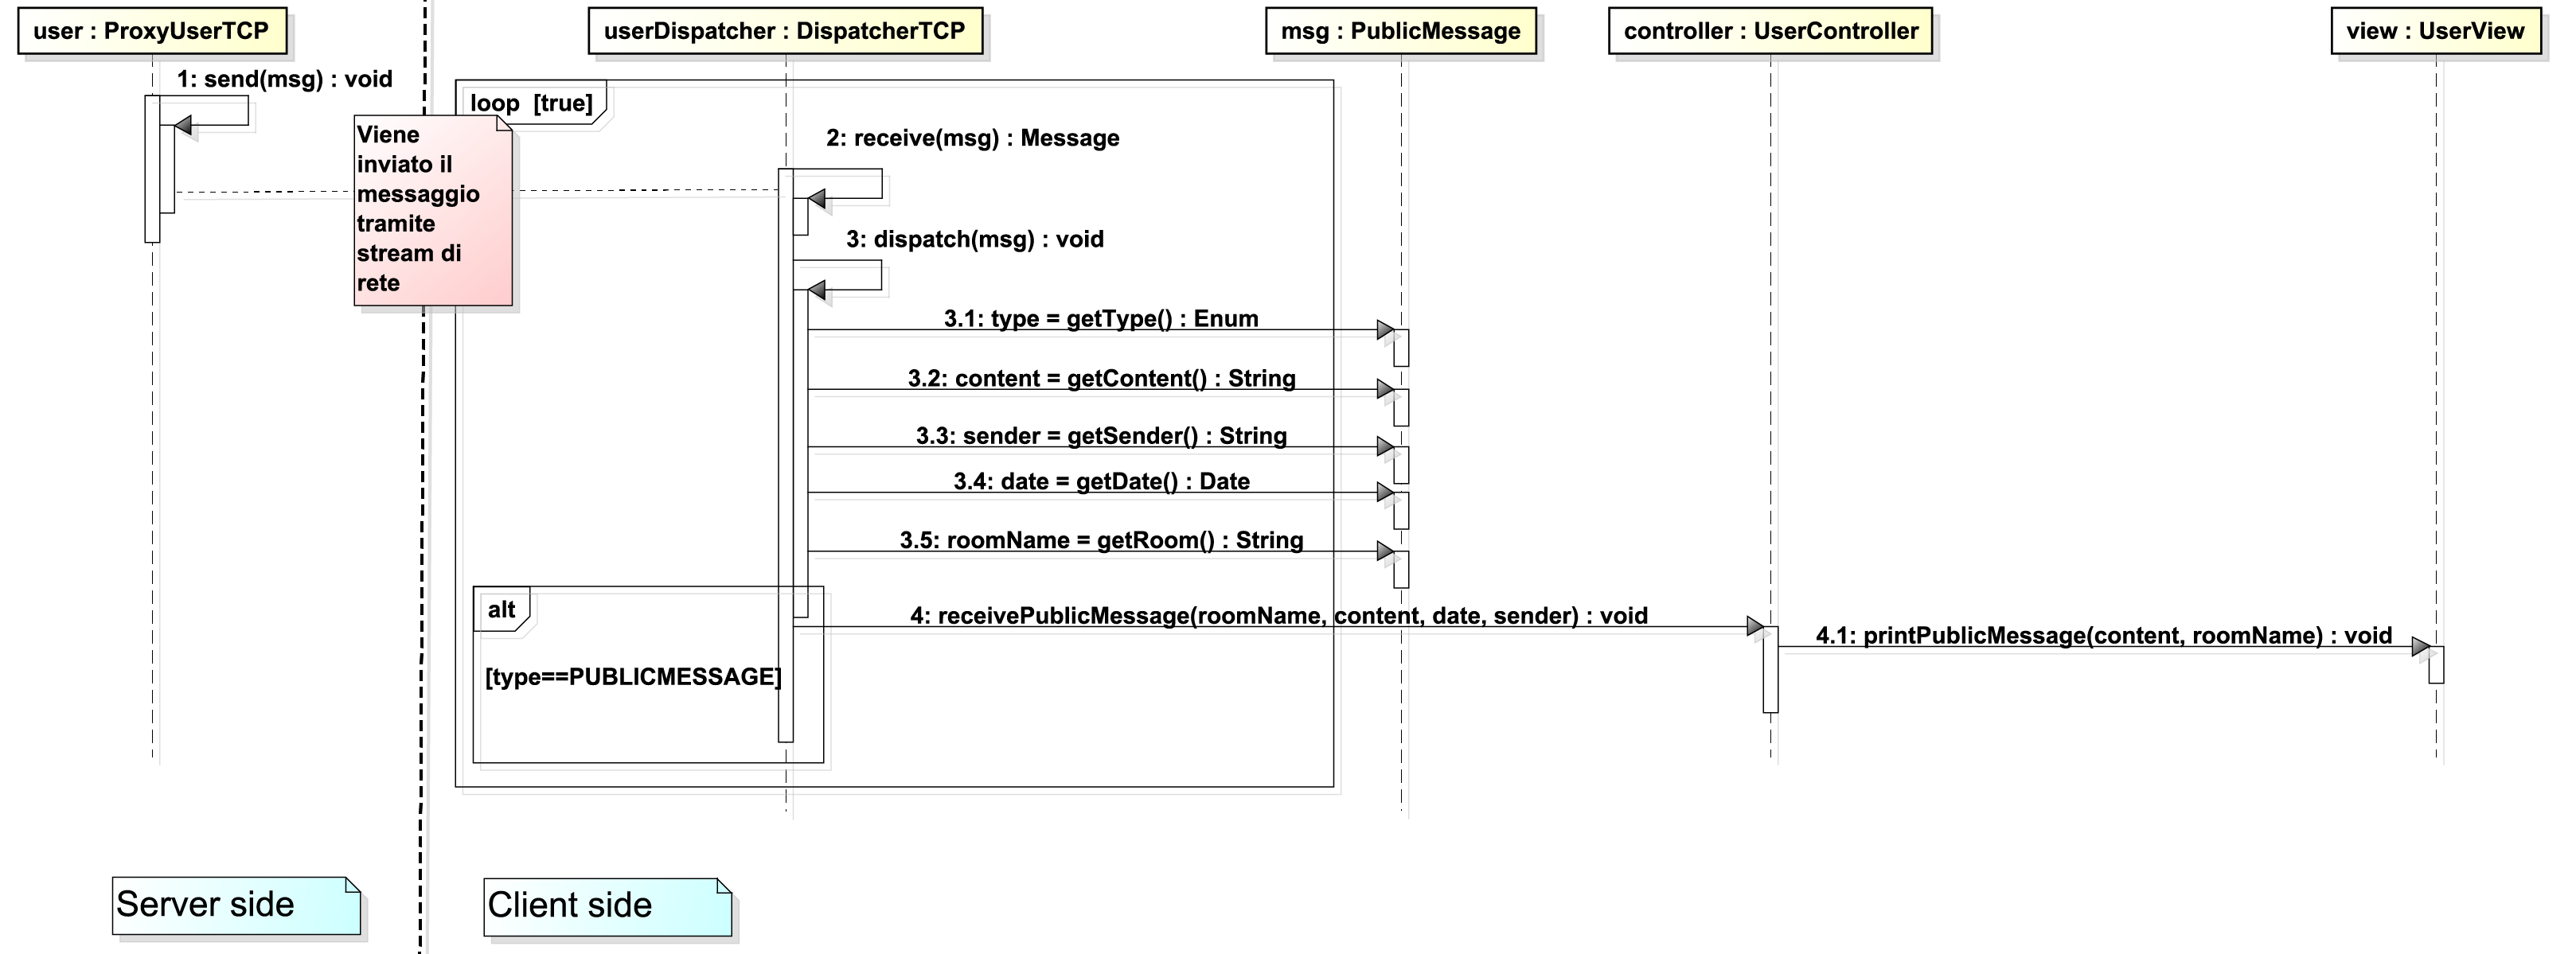
\includegraphics[scale=0.14]{image_astah/Iteration_2_DesignModel/UC3_SendPublicMessage_SSD_3_receiveMsg.png}{\centering}
     \caption{SSD - OP3: receive(msg) del modello di dominio (figura \ref{fig_UC3_SPM_SSD})}
     \label{fig_UC3_SSD_SRM_3} 
   \end{figure}
\end{frame}

\subsection{Iterazione 2: Implementazione - UC3\_SendPublicMessage}
\begin{frame} {Iterazione 2: Implementazione - UC3\_SendPublicMessage}
  \emph{INSERIRE DESCRIZIONE}
\end{frame}

% ELABORAZIONE ITERAZIONE 3 - UC4\_SendPrivateMessage
\section{Elaborazione - Iterazione 3}
\begin{frame} {Descrizione Elaborazione: Iterazione 3}
  \emph{INSERIRE DESCRIZIONE}
\end{frame}

\subsection {Iterazione 3: Requisiti - UC4\_SendPrivateMessage}
\begin{frame} {Iterazione 3: Requisiti - UC4\_SendPrivateMessage}
  \begin{table}[!htbp]
    \caption {Caso d'uso UC4\_SendPrivateMessage}
     \label{table_UC4_SPM}
      \resizebox{\linewidth}{!}{%
       \begin{tabular}{|l|p{10cm}|}\hline
        Nome caso d'uso &  UC3\_SendRoomMessage\\\hline
        Portata & Applicazione Smart Intelligent University Communications \\\hline
        Livello & Obiettivo Utente \\\hline
        Attore primario & SnucUser  \\\hline
        Parti interessate e interessi & SnucUser: vuole che i messaggi siano inviati all’utente selezionato presente nella stanza virtuale \\\hline
        Pre-condizioni &  L'utente è registrato nella stanza in cui desidera inviare un messaggio ad un altro utente presente \\\hline
        Post-condizioni (garanzia di successo) & L'utente selezionato riceve il messaggio inviato \\\hline
         Scenario principale di successo &  
         \begin{enumerate} 
          \item L’utente seleziona il destinatario del messaggio privato.
          \item L’utente inserisce da tastiera il messaggio da inviare.
	  \item Il messaggio viene inoltrato al destinatario selezionato.
         \end{enumerate} \\\hline
      \end{tabular}}
   \end{table}
\end{frame}

\begin{frame} {Iterazione 3: Requisiti - UC4\_SendPrivateMessage}
  \begin{table}[!htbp]
      \resizebox{\linewidth}{!}{%
       \begin{tabular}{|l|p{10cm}|}\hline
         Requisiti speciali (Requisiti Non Funzionali) &  Comunicazione asincrona in cui lo scambio di informazioni avviene in tempo reale, senza sensibili pause tra 
                                                        invio e ricezione del messaggio\\\hline
         Elenco delle varianti tecnologiche &  
          \begin{itemize}  
           \item \`E possibile inviare messaggi confidenziali, autenticati e integri al server del servizio di messaggistica.
           \item L’applicazione dovrebbe essere flessibile al funzionamento di diversi protocolli di comunicazione (es. TCP, UDP) e con diversi strati middleware 
                 (es. Socket, RMI)
          \end{itemize} \\\hline
         Frequenza di ripetizione & Potrebbe essere quasi ininterrotta \\\hline
         Varie e/o Problemi Aperti &  // \\\hline
      \end{tabular}}
   \end{table}
\end{frame}

\subsection {Iterazione 3: Analisi - UC4\_SendPrivateMessage}
\begin{frame} [allowframebreaks] {Descrizione Iterazione 3: Analisi - UC4\_SendPrivateMessage}
  In questa iterazione, del caso d’uso UC4 è di interesse lo scenario principale di successo.  Da esso è possibile identificare le seguenti classi concettuali: 
  \begin{itemize}
   \item \textbf{User}: rappresenta il generico utente, caratterizzato da un ``nickname'', connesso al servizio di messaggistica. Può richiedere la lista delle 
         stanze, ricevere notifiche dal sistema centrale. Interagisce con il MessagingSevice richiedendo la registrazione e l’ingresso in una specifica stanza. 
         Può inviare messaggi pubblici e \textit{privati}.
   \item \textbf{MessagingService}: rappresenta ed incapsula il servizio di messaggistica nel suo complesso. Mantiene una lista di utenti connessi a tale sistema. 
          Mantiene una lista di stanze e riceve tramite comandi richieste di ingresso da parte degli utenti. Svolge il ruolo di smistatore di messaggi inviati dagli 
          User.
   \item \textbf{Message}: individua un generico messaggio scambiato tra utenti della chat o tra servizio di messaggistica e utente. È costituito da un 
         ``content'' (contenuto del messaggio) , da una ``date'' (rappresenta la data) e dal ``sender'' (mittente).
   \item \textbf{Notify}: è una specializzazione del tipo Message ed è caratterizzata da un typeNotify che serve a distinguere il tipo di notifica (ad es. 
          CONNECTIO\_ACCEPT nel caso in cui la connessione è stata stabilita correttamente, BAD\_COMMAND nel caso in cui il comando inviato dall'User non 
          sia riconosciuto dal Server).
   \item \textbf{PublicNotify}: è una specializzazione di Notify e questo tipo di notifica viene ricevuta da tutti gli utenti registrati alla relativa 
          stanza. Un esempio di PublicNotify è la notifica caratterizzata dal seguente typeNotify: UPDATE\_LIST\_USERS, grazie alla quale viene 
          aggiornata la lista degli utenti registrati nella relativa stanza.
   \item  \textbf{Commad}: è una specializzazione di Message e rappresenta il comando che viene inviato dall'User e ricevuto ed interpretato dal            
          MessagingService (es. /join '\#Medical' richiesta da parte dell'utente a registrarsi alla stanza Medical).        
   \item \textbf{Room}: è caratterizzata da un nome. Ciascuna istanza individua una specifica stanza nella chat.
   \item \textbf{Register}: mantiene un riferimento all’insieme di partecipanti che in un certo istante sono presenti nella stanza.
   \item \textbf{PublicMessage}: è una specializzazione di Message ed individua un messaggio pubblico scambiato tra utenti della chat registrati nella 
         stessa stanza. 
   \item \textit{\textbf{PrivateMessage}: una specializzazione di Message ed individua un messaggio privato scambiato tra due utenti della chat registrati nella  
         stessa stanza}. 
  \end{itemize}
\end{frame}

\begin{frame} {Iterazione 3: Analisi - UC4\_SendPrivateMessage}
   \begin{figure}
     \includegraphics[scale=0.16]{image_astah/Iteration_3_DomainModel/UC4_SendPrivateMessage_DM.png}{\centering}
     \caption{UC3 - Modello di dominio}
     \label{fig_UC4_SPM_DM} 
   \end{figure}
\end{frame}

\begin{frame} {Iterazione 3: Analisi - UC4\_SendPrivateMessage}
   \begin{figure}
     \includegraphics[scale=0.22]{image_astah/Iteration_3_DomainModel/UC4_SendPrivateMessage_OM.png}{\centering}
     \caption{UC3 - Oggetti di dominio}
     \label{fig_UC4_SPM_OM} 
   \end{figure}
\end{frame}

\begin{frame} {Iterazione 3: Analisi - UC4\_SendPrivateMessage}
   \begin{figure}
     \includegraphics[scale=0.28]{image_astah/Iteration_3_DomainModel/UC4_SendPrivateMessage_SSD.png}{\centering}
     \caption{UC4 - Diagramma di sequenza di sistema}
     \label{fig_UC4_SPM_SSD} 
   \end{figure}
\end{frame}

\begin{frame}
 \frametitle{Iterazione 3: Analisi, UC4 contratto CO6 }
  \begin{table}[!htbp]
   \caption {UC3 Contratto CO6 - privateMsg}
    \label{table_CO6}
      \resizebox{\linewidth}{!}{%
       \begin{tabular}{|l|p{10cm}|}\hline
         Operazione & \textit{privateMsg(msg:PublicMessage)} \\\hline 
         Riferimenti & Caso d’uso: UC4\_SendPrivateMessage \\\hline
         Pre-condizione & 
         \begin{itemize}
          \item L'utente è registrato nella stanza
          \item L'utente seleziona il destinatario del messaggio privato tra gli utenti registrati nella stanza    
         \end{itemize} \\\hline 
         Post-condizione & Il destinatario riceve il messaggio privato  \\\hline
      \end{tabular}}
   \end{table}
\end{frame}

\subsection{Iterazione 3: Progettazione}
\begin{frame} {Descrizione Iterazione 3: Progettazione}
  \emph{INSERIRE DESCRIZIONE}
\end{frame}

\subsection{Iterazione 3: Progettazione Class Diagram UC4\_SendPrivateMessage}
\begin{frame} {Iterazione 3: Progettazione Class Diagram Common UC4}
   \begin{figure}
     \includegraphics[scale=0.15]{image_astah/Iteration_3_DesignModel/ClassDiagramCommon.png}{\centering}
     \caption{DCD - Diagramma delle Classi: Package Common }
     \label{fig_UC4_DCD_1} 
   \end{figure}
\end{frame}

\begin{frame} {Iterazione 3: Progettazione Class Diagram Snuc UC4}
   \begin{figure}
     \includegraphics[scale=0.16]{image_astah/Iteration_3_DesignModel/ClassDiagramSnuc.png}{\centering}
     \caption{DCD - Diagramma delle Classi: Package Snuc }
     \label{fig_UC4_DCD_3} 
   \end{figure}
\end{frame}

\begin{frame} {Iterazione 3: Progettazione Class Diagram Connector UC4}
   \begin{figure}
     \includegraphics[scale=0.077]{image_astah/Iteration_3_DesignModel/ClassDiagramConnector.png}{\centering}
     \caption{DCD - Diagramma delle Classi: Package Connector }
     \label{fig_UC4_DCD_4} 
   \end{figure}
\end{frame}

\begin{frame} {Iterazione 3: Progettazione Class Diagram Snuc Server UC4}
   \begin{figure}
     \includegraphics[scale=0.155]{image_astah/Iteration_3_DesignModel/ClassDiagramSnucServer.png}{\centering}
     \caption{DCD - Diagramma delle Classi: Package Snuc Server }
     \label{fig_UC4_DCD_2} 
   \end{figure}
\end{frame}

\subsection{Iterazione 3: Progettazione - SSD UC4\_SendPrivateMessage}
\begin{frame} {Iterazione 3: Progettazione, UC4\_SendPrivateMessage - OP1}
   \begin{figure}
     \includegraphics[scale=0.16]{image_astah/Iteration_3_DesignModel/UC4_SendPrivateMessage_SSD_1_sendMsg.png}{\centering}
     \caption{SSD - OP1: sendMsg(msg) del modello di dominio (figura \ref{fig_UC4_SPM_SSD}) }
     \label{fig_UC4_SSD_SRM_1} 
   \end{figure}
\end{frame}

\begin{frame} {Iterazione 3: Progettazione, UC4\_SendPrivateMessage - OP2}
   \begin{figure}
     \includegraphics[scale=0.105]{image_astah/Iteration_3_DesignModel/UC4_SendPrivateMessage_SSD_2_privateMsg}{\centering}
     \caption{SSD - OP2: privateMsg(msg) del modello di dominio (figura \ref{fig_UC4_SPM_SSD}) }
     \label{fig_UC4_SSD_SRM_2} 
   \end{figure}
\end{frame}

\begin{frame} {Iterazione 3: Progettazione, UC4\_SendPrivateMessage - OP3}
   \begin{figure}
     \includegraphics[scale=0.14]{image_astah/Iteration_3_DesignModel/UC4_SendPrivateMessage_SSD_3_receive.png}{\centering}
     \caption{SSD - OP3: receive(msg) del modello di dominio (figura \ref{fig_UC4_SPM_SSD})}
     \label{fig_UC4_SSD_SRM_3} 
   \end{figure}
\end{frame}


\subsection {Iterazione 3: Implementazione - UC4\_SendPrivateMessage}
\begin{frame} {Iterazione 3: Implementazione - UC4\_SendPrivateMessage}
 \emph{INSERIRE DESCRIZIONE}
\end{frame}

\section {Riferimenti}
\subsection {Bibliografia e Sitografia}
\begin {frame} [allowframebreaks] 
  \frametitle {Bigliografia e Sitografia}
% \frametitle {\refname}
  \begin {thebibliography}{99}
   {\tiny 
     \setbeamertemplate{bibliography item}[book]
     \bibitem {bib0} Herbert Schildt
     \newblock \emph{Java SE 7. La guida completa.} 
     \newblock {McGraw-Hill, 2012}

     \bibitem {bib1}  Martin Fowler, L. Baresi, S. Gaburri 
     \newblock \emph{UML distilled. Guida rapida al linguaggio di modellazione standard} 
     \newblock {Pearson Education Italia, 2010}

     \bibitem {bib2} Craig Larman, Luca Cabibbo
     \newblock \emph{Applicare UML e i pattern: analisi e progettazione orientata agli oggetti} 
     \newblock {Pearson Education Italia, 2005}

     \bibitem {bib3} M.L. Liu
     \newblock \emph{Distributed Computing: Principles and Applications} 
     \newblock {Addison-Wesley, 2003}

     \bibitem {bib4} Erich Gamma, Richard Helm, Ralph Johnson, John Vlissides
     \newblock \emph{Design patterns - Elementi per il riuso di software ad oggetti} 
     \newblock {Pearson Education Italia, 1995}
      
     \setbeamertemplate{bibliography item}[online]
     \bibitem {bib5} Pattern GOF - Giuseppe Dell'Abate's Blog
     \newblock Riferimenti: \emph{\url{https://dellabate.wordpress.com/category/gof-pattern/ }}

     \setbeamertemplate{bibliography item}[online]
     \bibitem {bib6} Test unità con Junit4
     \newblock Riferimenti: \emph{\url{http://junit.org }}

     \setbeamertemplate{bibliography item}[online]
     \bibitem {bib7} The Java Tutorials 
     \newblock Riferimenti: \emph{\url{http://docs.oracle.com/javase/tutorial/ }}

     \setbeamertemplate{bibliography item}[online]
     \bibitem {bib8} Java Platform, Standard Edition 8 API Specification 
     \newblock Riferimenti: \emph{\url{http://docs.oracle.com/javase/8/docs/api/ }}

     \setbeamertemplate{bibliography item}[online]
     \bibitem {bib9} Git --everything-is-local  
     \newblock Riferimenti: \emph{\url{http://git-scm.com/ }}

     \setbeamertemplate{bibliography item}[online]
     \bibitem {bib10} git - la guida tascabile 
     \newblock Riferimenti: \emph{\url{http://rogerdudler.github.io/git-guide/index.it.html }}

     \setbeamertemplate{bibliography item}[online]
     \bibitem {bib11} Astah.net: UML and Modeling Tools
     \newblock Riferimenti: \emph{\url{http://astah.net/ }}

     \setbeamertemplate{bibliography item}[online]
     \bibitem {bib11} NetBeans Documentation
     \newblock Riferimenti: \emph{\url{https://netbeans.org/kb/docs/java/quickstart.html }}

   }
   \end {thebibliography}
\end {frame}
\end{document}
